\documentclass[letterpaper,12pt]{article}
\usepackage[english]{babel}
\usepackage[utf8x]{inputenc}
\usepackage[T1]{fontenc}
\usepackage{titlesec}
\usepackage[letterpaper,top=1in,bottom=1in,left=1in,right=1in,marginparwidth=0in]{geometry}
\usepackage{times}
\usepackage{amsmath}
\usepackage{graphicx}
\usepackage[colorlinks=true, allcolors=blue]{hyperref}
\usepackage{enumitem} 
\usepackage{natbib} 
\usepackage{libertine}
\usepackage{float}
\begin{document}
\fontfamily{ptm}\selectfont
\urlstyle{same}
\urlstyle{rm}
\tableofcontents
\pagebreak




% Time series for each predictor variable 

\subsection{ML Inputs (with NAs) Time Series Images} 
 

\begin{figure} 
\centering  
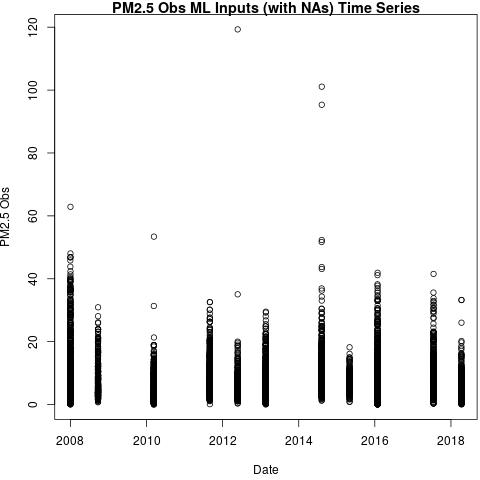
\includegraphics[width=0.77\textwidth]{Code_Outputs/Report_ML_input_PM25_Step4_part_e_de_duplicated_aves_compiled_2019-05-18wNAs_PM25_ObsvDate.jpg} 
\caption{\label{fig:Report_ML_input_PM25_Step4_part_e_de_duplicated_aves_compiled_2019-05-18wNAsPM25_ObsvDate}ML Inputs (with NAs) Time Series} 
\end{figure} 
 

\begin{figure} 
\centering  
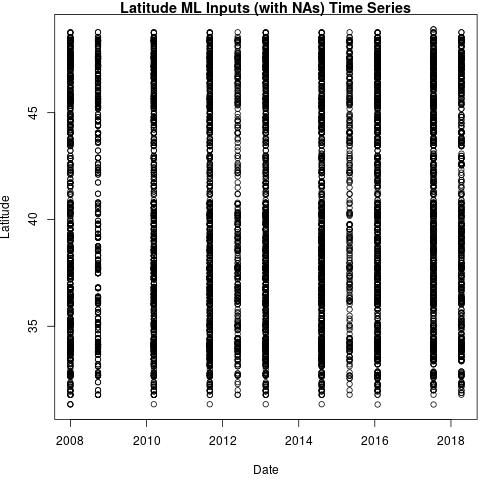
\includegraphics[width=0.77\textwidth]{Code_Outputs/Report_ML_input_PM25_Step4_part_e_de_duplicated_aves_compiled_2019-05-18wNAs_LatitudevDate.jpg} 
\caption{\label{fig:Report_ML_input_PM25_Step4_part_e_de_duplicated_aves_compiled_2019-05-18wNAsLatitudevDate}ML Inputs (with NAs) Time Series} 
\end{figure} 
 

\begin{figure} 
\centering  
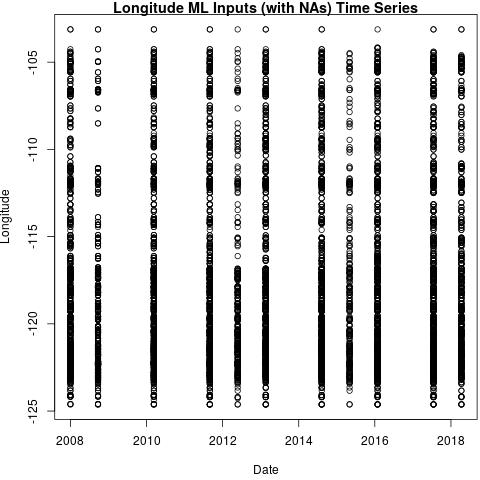
\includegraphics[width=0.77\textwidth]{Code_Outputs/Report_ML_input_PM25_Step4_part_e_de_duplicated_aves_compiled_2019-05-18wNAs_LongitudevDate.jpg} 
\caption{\label{fig:Report_ML_input_PM25_Step4_part_e_de_duplicated_aves_compiled_2019-05-18wNAsLongitudevDate}ML Inputs (with NAs) Time Series} 
\end{figure} 
 

\begin{figure} 
\centering  
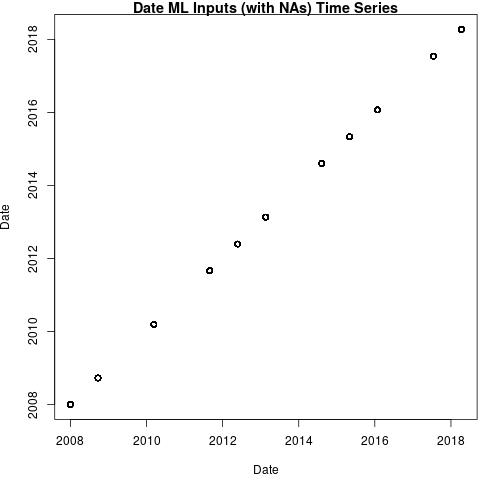
\includegraphics[width=0.77\textwidth]{Code_Outputs/Report_ML_input_PM25_Step4_part_e_de_duplicated_aves_compiled_2019-05-18wNAs_DatevDate.jpg} 
\caption{\label{fig:Report_ML_input_PM25_Step4_part_e_de_duplicated_aves_compiled_2019-05-18wNAsDatevDate}ML Inputs (with NAs) Time Series} 
\end{figure} 
 

\begin{figure} 
\centering  
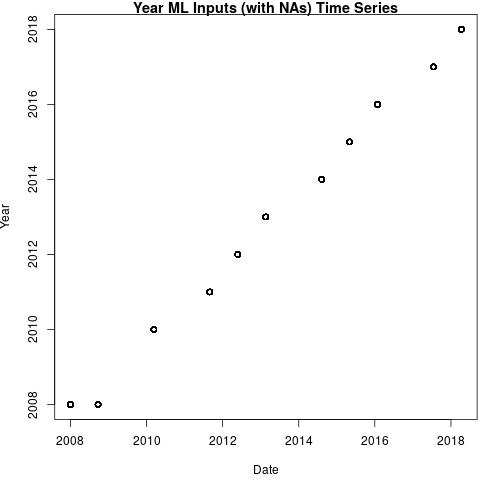
\includegraphics[width=0.77\textwidth]{Code_Outputs/Report_ML_input_PM25_Step4_part_e_de_duplicated_aves_compiled_2019-05-18wNAs_YearvDate.jpg} 
\caption{\label{fig:Report_ML_input_PM25_Step4_part_e_de_duplicated_aves_compiled_2019-05-18wNAsYearvDate}ML Inputs (with NAs) Time Series} 
\end{figure} 
 

\begin{figure} 
\centering  
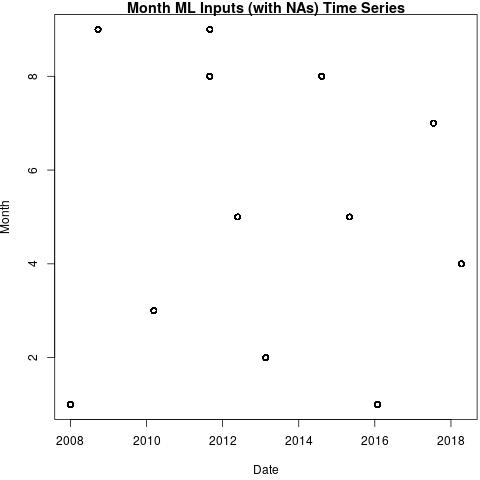
\includegraphics[width=0.77\textwidth]{Code_Outputs/Report_ML_input_PM25_Step4_part_e_de_duplicated_aves_compiled_2019-05-18wNAs_MonthvDate.jpg} 
\caption{\label{fig:Report_ML_input_PM25_Step4_part_e_de_duplicated_aves_compiled_2019-05-18wNAsMonthvDate}ML Inputs (with NAs) Time Series} 
\end{figure} 
 

\begin{figure} 
\centering  
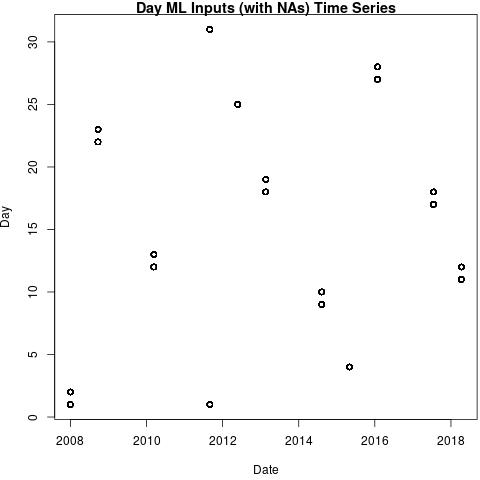
\includegraphics[width=0.77\textwidth]{Code_Outputs/Report_ML_input_PM25_Step4_part_e_de_duplicated_aves_compiled_2019-05-18wNAs_DayvDate.jpg} 
\caption{\label{fig:Report_ML_input_PM25_Step4_part_e_de_duplicated_aves_compiled_2019-05-18wNAsDayvDate}ML Inputs (with NAs) Time Series} 
\end{figure} 
 

\begin{figure} 
\centering  
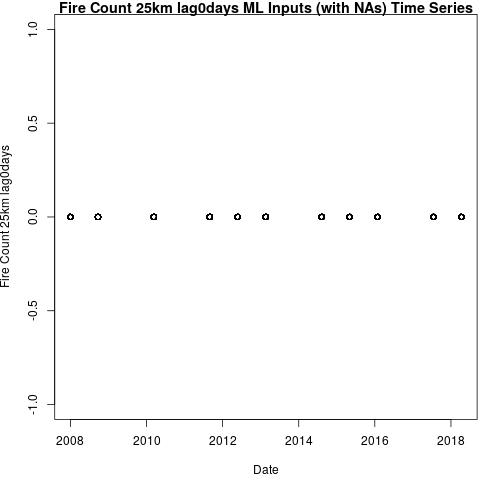
\includegraphics[width=0.77\textwidth]{Code_Outputs/Report_ML_input_PM25_Step4_part_e_de_duplicated_aves_compiled_2019-05-18wNAs_Fire_Count_25km_lag0daysvDate.jpg} 
\caption{\label{fig:Report_ML_input_PM25_Step4_part_e_de_duplicated_aves_compiled_2019-05-18wNAsFire_Count_25km_lag0daysvDate}ML Inputs (with NAs) Time Series} 
\end{figure} 
 

\begin{figure} 
\centering  
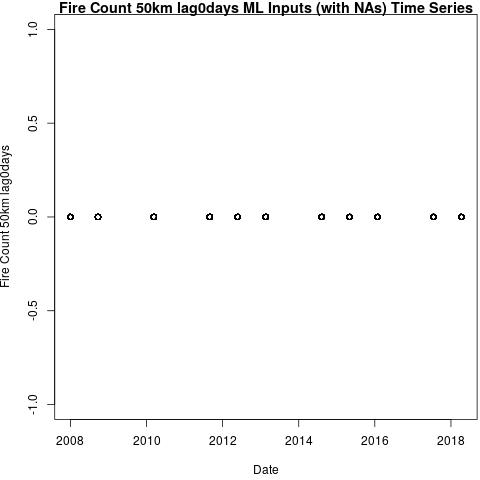
\includegraphics[width=0.77\textwidth]{Code_Outputs/Report_ML_input_PM25_Step4_part_e_de_duplicated_aves_compiled_2019-05-18wNAs_Fire_Count_50km_lag0daysvDate.jpg} 
\caption{\label{fig:Report_ML_input_PM25_Step4_part_e_de_duplicated_aves_compiled_2019-05-18wNAsFire_Count_50km_lag0daysvDate}ML Inputs (with NAs) Time Series} 
\end{figure} 
 

\clearpage 

\begin{figure} 
\centering  
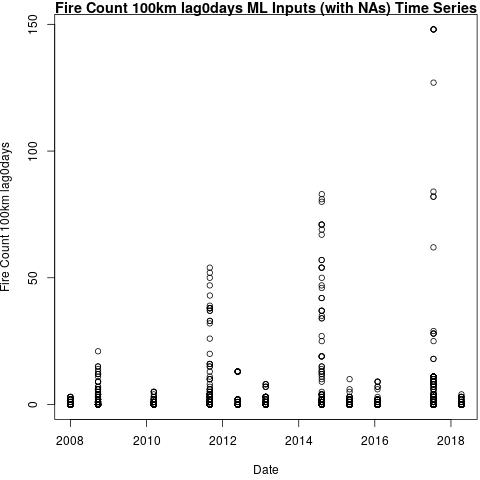
\includegraphics[width=0.77\textwidth]{Code_Outputs/Report_ML_input_PM25_Step4_part_e_de_duplicated_aves_compiled_2019-05-18wNAs_Fire_Count_100km_lag0daysvDate.jpg} 
\caption{\label{fig:Report_ML_input_PM25_Step4_part_e_de_duplicated_aves_compiled_2019-05-18wNAsFire_Count_100km_lag0daysvDate}ML Inputs (with NAs) Time Series} 
\end{figure} 
 

\begin{figure} 
\centering  
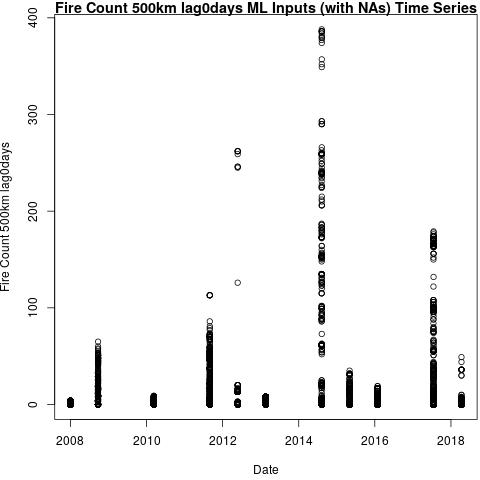
\includegraphics[width=0.77\textwidth]{Code_Outputs/Report_ML_input_PM25_Step4_part_e_de_duplicated_aves_compiled_2019-05-18wNAs_Fire_Count_500km_lag0daysvDate.jpg} 
\caption{\label{fig:Report_ML_input_PM25_Step4_part_e_de_duplicated_aves_compiled_2019-05-18wNAsFire_Count_500km_lag0daysvDate}ML Inputs (with NAs) Time Series} 
\end{figure} 
 

\begin{figure} 
\centering  
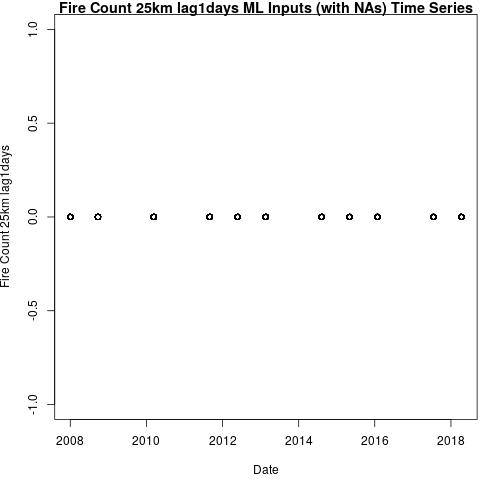
\includegraphics[width=0.77\textwidth]{Code_Outputs/Report_ML_input_PM25_Step4_part_e_de_duplicated_aves_compiled_2019-05-18wNAs_Fire_Count_25km_lag1daysvDate.jpg} 
\caption{\label{fig:Report_ML_input_PM25_Step4_part_e_de_duplicated_aves_compiled_2019-05-18wNAsFire_Count_25km_lag1daysvDate}ML Inputs (with NAs) Time Series} 
\end{figure} 
 

\begin{figure} 
\centering  
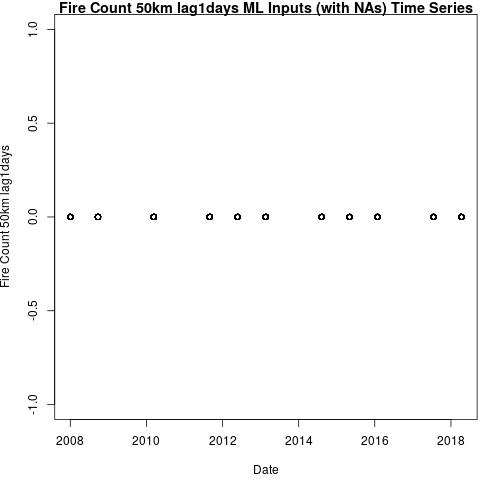
\includegraphics[width=0.77\textwidth]{Code_Outputs/Report_ML_input_PM25_Step4_part_e_de_duplicated_aves_compiled_2019-05-18wNAs_Fire_Count_50km_lag1daysvDate.jpg} 
\caption{\label{fig:Report_ML_input_PM25_Step4_part_e_de_duplicated_aves_compiled_2019-05-18wNAsFire_Count_50km_lag1daysvDate}ML Inputs (with NAs) Time Series} 
\end{figure} 
 

\begin{figure} 
\centering  
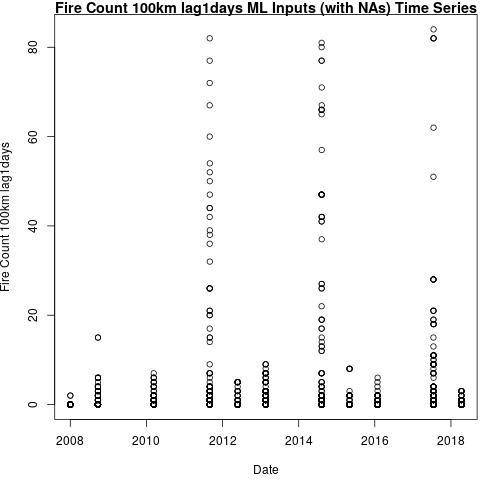
\includegraphics[width=0.77\textwidth]{Code_Outputs/Report_ML_input_PM25_Step4_part_e_de_duplicated_aves_compiled_2019-05-18wNAs_Fire_Count_100km_lag1daysvDate.jpg} 
\caption{\label{fig:Report_ML_input_PM25_Step4_part_e_de_duplicated_aves_compiled_2019-05-18wNAsFire_Count_100km_lag1daysvDate}ML Inputs (with NAs) Time Series} 
\end{figure} 
 

\begin{figure} 
\centering  
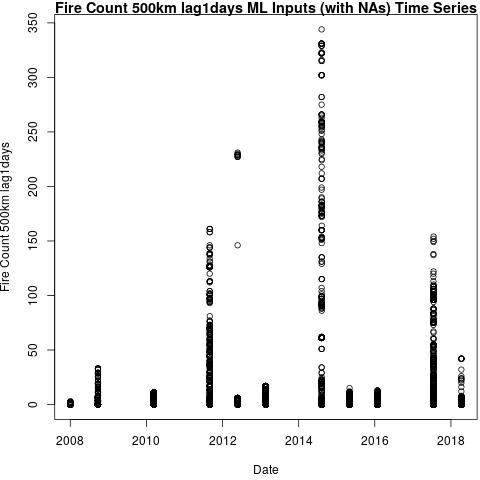
\includegraphics[width=0.77\textwidth]{Code_Outputs/Report_ML_input_PM25_Step4_part_e_de_duplicated_aves_compiled_2019-05-18wNAs_Fire_Count_500km_lag1daysvDate.jpg} 
\caption{\label{fig:Report_ML_input_PM25_Step4_part_e_de_duplicated_aves_compiled_2019-05-18wNAsFire_Count_500km_lag1daysvDate}ML Inputs (with NAs) Time Series} 
\end{figure} 
 

\begin{figure} 
\centering  
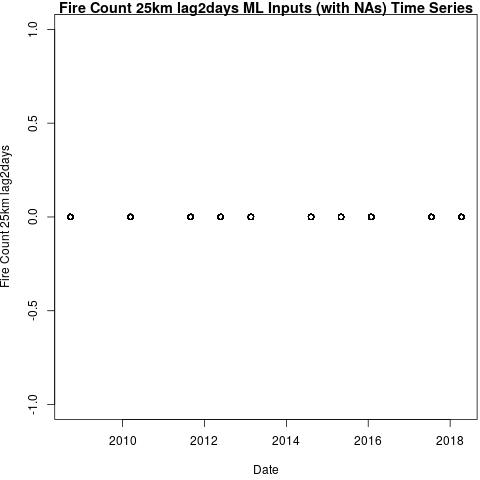
\includegraphics[width=0.77\textwidth]{Code_Outputs/Report_ML_input_PM25_Step4_part_e_de_duplicated_aves_compiled_2019-05-18wNAs_Fire_Count_25km_lag2daysvDate.jpg} 
\caption{\label{fig:Report_ML_input_PM25_Step4_part_e_de_duplicated_aves_compiled_2019-05-18wNAsFire_Count_25km_lag2daysvDate}ML Inputs (with NAs) Time Series} 
\end{figure} 
 

\begin{figure} 
\centering  
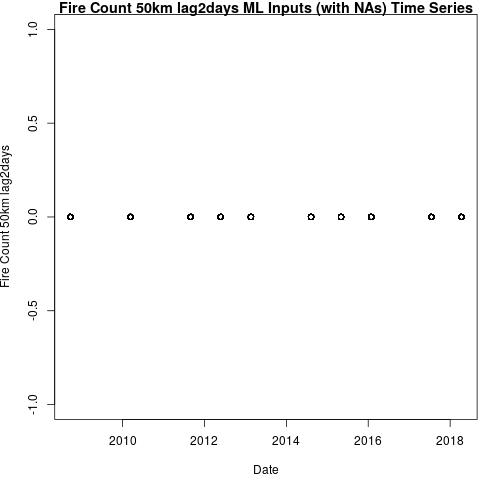
\includegraphics[width=0.77\textwidth]{Code_Outputs/Report_ML_input_PM25_Step4_part_e_de_duplicated_aves_compiled_2019-05-18wNAs_Fire_Count_50km_lag2daysvDate.jpg} 
\caption{\label{fig:Report_ML_input_PM25_Step4_part_e_de_duplicated_aves_compiled_2019-05-18wNAsFire_Count_50km_lag2daysvDate}ML Inputs (with NAs) Time Series} 
\end{figure} 
 

\begin{figure} 
\centering  
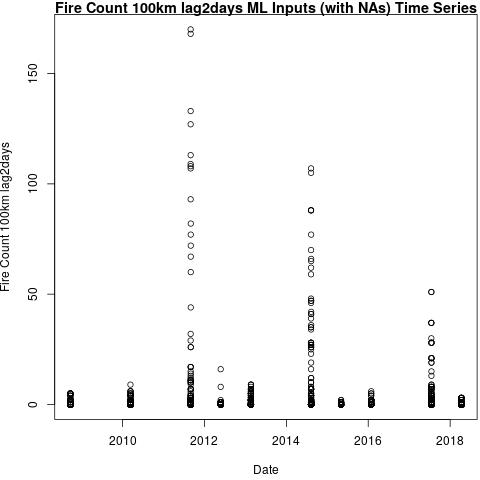
\includegraphics[width=0.77\textwidth]{Code_Outputs/Report_ML_input_PM25_Step4_part_e_de_duplicated_aves_compiled_2019-05-18wNAs_Fire_Count_100km_lag2daysvDate.jpg} 
\caption{\label{fig:Report_ML_input_PM25_Step4_part_e_de_duplicated_aves_compiled_2019-05-18wNAsFire_Count_100km_lag2daysvDate}ML Inputs (with NAs) Time Series} 
\end{figure} 
 

\begin{figure} 
\centering  
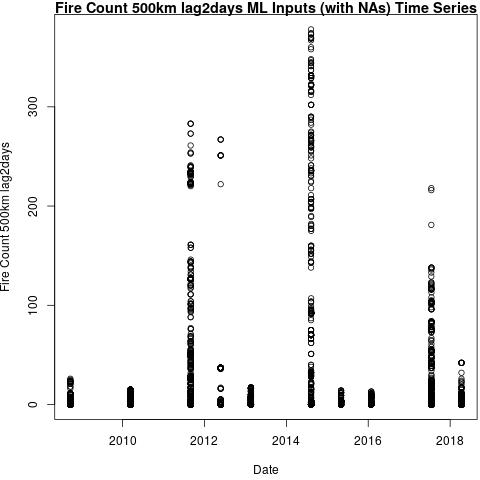
\includegraphics[width=0.77\textwidth]{Code_Outputs/Report_ML_input_PM25_Step4_part_e_de_duplicated_aves_compiled_2019-05-18wNAs_Fire_Count_500km_lag2daysvDate.jpg} 
\caption{\label{fig:Report_ML_input_PM25_Step4_part_e_de_duplicated_aves_compiled_2019-05-18wNAsFire_Count_500km_lag2daysvDate}ML Inputs (with NAs) Time Series} 
\end{figure} 
 

\clearpage 

\begin{figure} 
\centering  
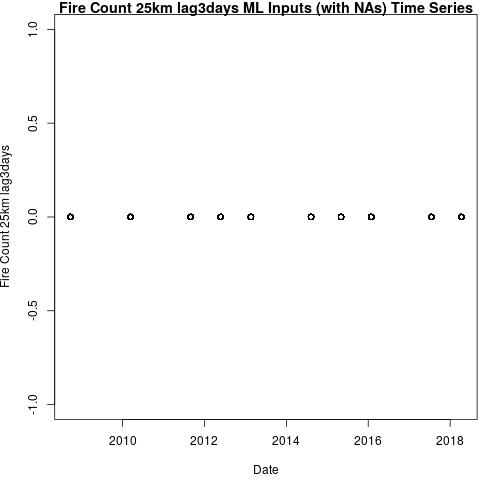
\includegraphics[width=0.77\textwidth]{Code_Outputs/Report_ML_input_PM25_Step4_part_e_de_duplicated_aves_compiled_2019-05-18wNAs_Fire_Count_25km_lag3daysvDate.jpg} 
\caption{\label{fig:Report_ML_input_PM25_Step4_part_e_de_duplicated_aves_compiled_2019-05-18wNAsFire_Count_25km_lag3daysvDate}ML Inputs (with NAs) Time Series} 
\end{figure} 
 

\begin{figure} 
\centering  
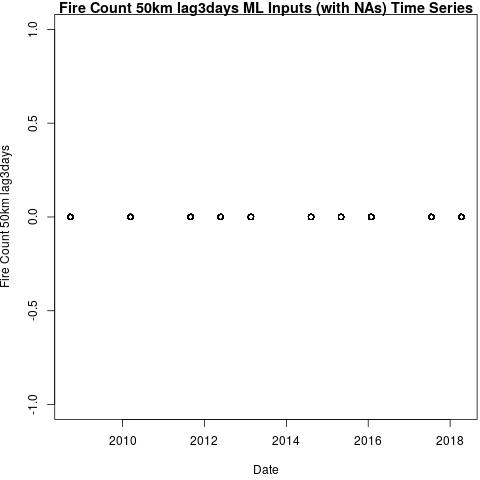
\includegraphics[width=0.77\textwidth]{Code_Outputs/Report_ML_input_PM25_Step4_part_e_de_duplicated_aves_compiled_2019-05-18wNAs_Fire_Count_50km_lag3daysvDate.jpg} 
\caption{\label{fig:Report_ML_input_PM25_Step4_part_e_de_duplicated_aves_compiled_2019-05-18wNAsFire_Count_50km_lag3daysvDate}ML Inputs (with NAs) Time Series} 
\end{figure} 
 

\begin{figure} 
\centering  
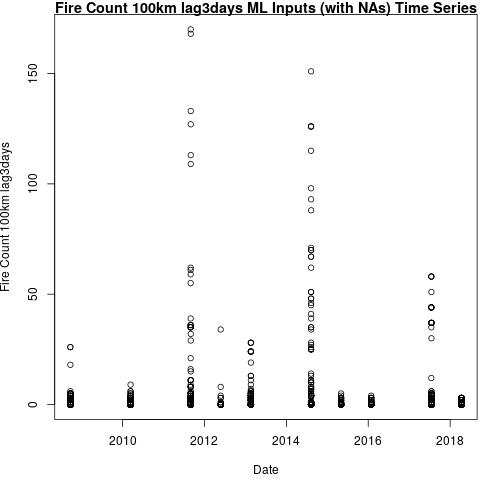
\includegraphics[width=0.77\textwidth]{Code_Outputs/Report_ML_input_PM25_Step4_part_e_de_duplicated_aves_compiled_2019-05-18wNAs_Fire_Count_100km_lag3daysvDate.jpg} 
\caption{\label{fig:Report_ML_input_PM25_Step4_part_e_de_duplicated_aves_compiled_2019-05-18wNAsFire_Count_100km_lag3daysvDate}ML Inputs (with NAs) Time Series} 
\end{figure} 
 

\begin{figure} 
\centering  
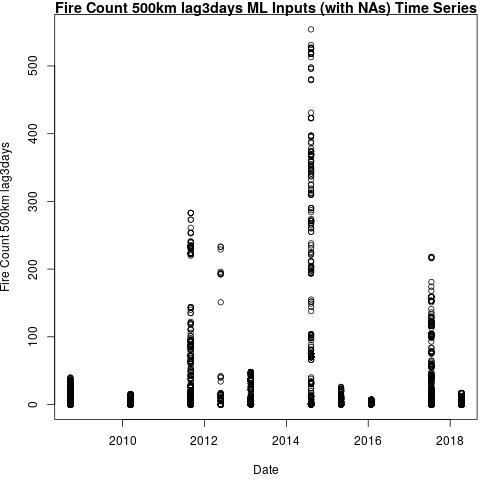
\includegraphics[width=0.77\textwidth]{Code_Outputs/Report_ML_input_PM25_Step4_part_e_de_duplicated_aves_compiled_2019-05-18wNAs_Fire_Count_500km_lag3daysvDate.jpg} 
\caption{\label{fig:Report_ML_input_PM25_Step4_part_e_de_duplicated_aves_compiled_2019-05-18wNAsFire_Count_500km_lag3daysvDate}ML Inputs (with NAs) Time Series} 
\end{figure} 
 

\begin{figure} 
\centering  
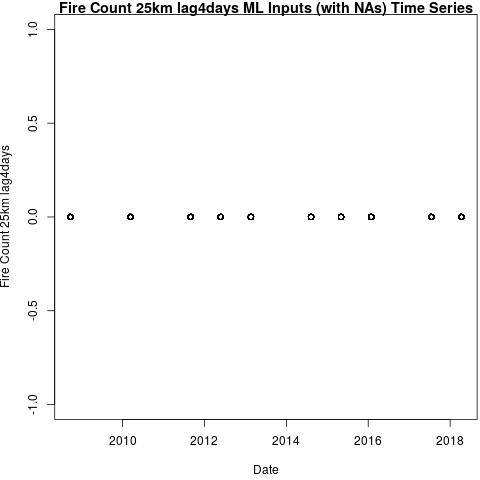
\includegraphics[width=0.77\textwidth]{Code_Outputs/Report_ML_input_PM25_Step4_part_e_de_duplicated_aves_compiled_2019-05-18wNAs_Fire_Count_25km_lag4daysvDate.jpg} 
\caption{\label{fig:Report_ML_input_PM25_Step4_part_e_de_duplicated_aves_compiled_2019-05-18wNAsFire_Count_25km_lag4daysvDate}ML Inputs (with NAs) Time Series} 
\end{figure} 
 

\begin{figure} 
\centering  
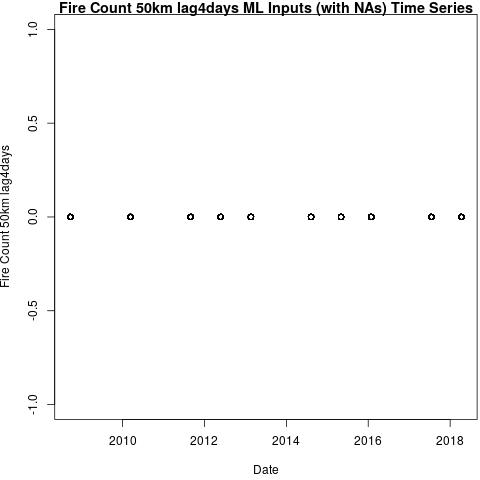
\includegraphics[width=0.77\textwidth]{Code_Outputs/Report_ML_input_PM25_Step4_part_e_de_duplicated_aves_compiled_2019-05-18wNAs_Fire_Count_50km_lag4daysvDate.jpg} 
\caption{\label{fig:Report_ML_input_PM25_Step4_part_e_de_duplicated_aves_compiled_2019-05-18wNAsFire_Count_50km_lag4daysvDate}ML Inputs (with NAs) Time Series} 
\end{figure} 
 

\begin{figure} 
\centering  
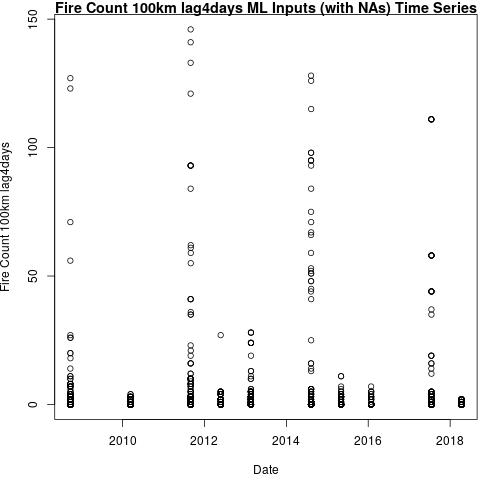
\includegraphics[width=0.77\textwidth]{Code_Outputs/Report_ML_input_PM25_Step4_part_e_de_duplicated_aves_compiled_2019-05-18wNAs_Fire_Count_100km_lag4daysvDate.jpg} 
\caption{\label{fig:Report_ML_input_PM25_Step4_part_e_de_duplicated_aves_compiled_2019-05-18wNAsFire_Count_100km_lag4daysvDate}ML Inputs (with NAs) Time Series} 
\end{figure} 
 

\begin{figure} 
\centering  
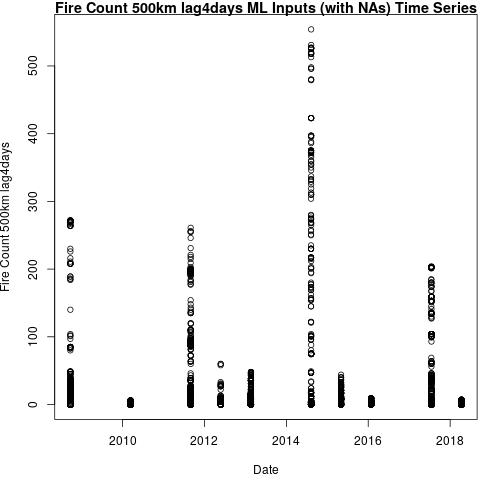
\includegraphics[width=0.77\textwidth]{Code_Outputs/Report_ML_input_PM25_Step4_part_e_de_duplicated_aves_compiled_2019-05-18wNAs_Fire_Count_500km_lag4daysvDate.jpg} 
\caption{\label{fig:Report_ML_input_PM25_Step4_part_e_de_duplicated_aves_compiled_2019-05-18wNAsFire_Count_500km_lag4daysvDate}ML Inputs (with NAs) Time Series} 
\end{figure} 
 

\begin{figure} 
\centering  
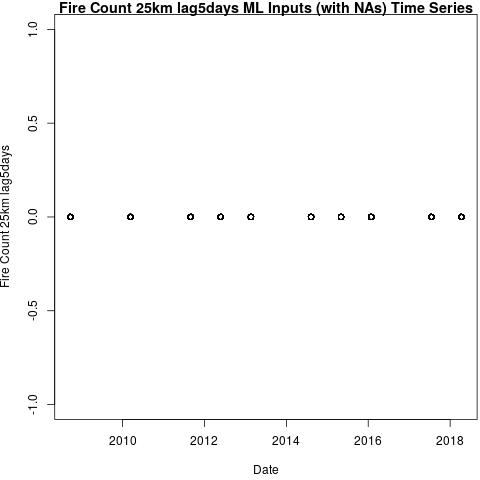
\includegraphics[width=0.77\textwidth]{Code_Outputs/Report_ML_input_PM25_Step4_part_e_de_duplicated_aves_compiled_2019-05-18wNAs_Fire_Count_25km_lag5daysvDate.jpg} 
\caption{\label{fig:Report_ML_input_PM25_Step4_part_e_de_duplicated_aves_compiled_2019-05-18wNAsFire_Count_25km_lag5daysvDate}ML Inputs (with NAs) Time Series} 
\end{figure} 
 

\begin{figure} 
\centering  
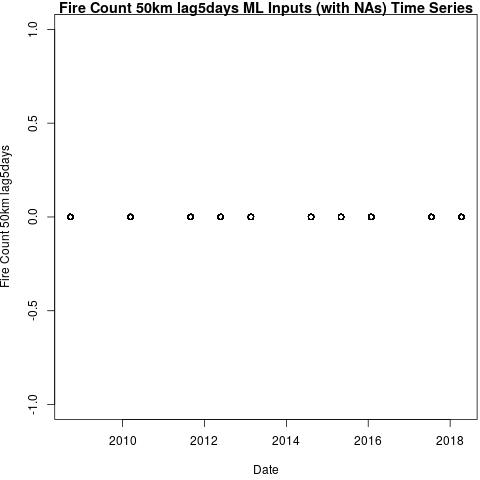
\includegraphics[width=0.77\textwidth]{Code_Outputs/Report_ML_input_PM25_Step4_part_e_de_duplicated_aves_compiled_2019-05-18wNAs_Fire_Count_50km_lag5daysvDate.jpg} 
\caption{\label{fig:Report_ML_input_PM25_Step4_part_e_de_duplicated_aves_compiled_2019-05-18wNAsFire_Count_50km_lag5daysvDate}ML Inputs (with NAs) Time Series} 
\end{figure} 
 

\clearpage 

\begin{figure} 
\centering  
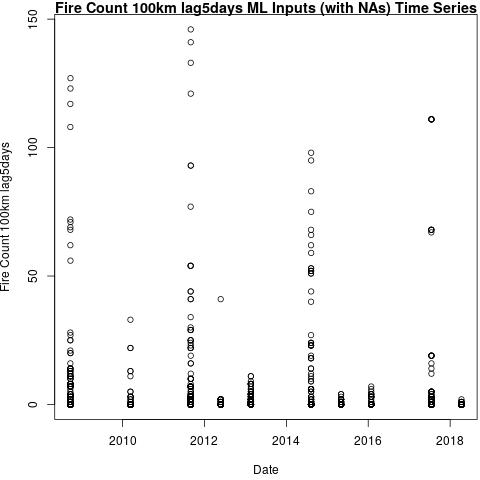
\includegraphics[width=0.77\textwidth]{Code_Outputs/Report_ML_input_PM25_Step4_part_e_de_duplicated_aves_compiled_2019-05-18wNAs_Fire_Count_100km_lag5daysvDate.jpg} 
\caption{\label{fig:Report_ML_input_PM25_Step4_part_e_de_duplicated_aves_compiled_2019-05-18wNAsFire_Count_100km_lag5daysvDate}ML Inputs (with NAs) Time Series} 
\end{figure} 
 

\begin{figure} 
\centering  
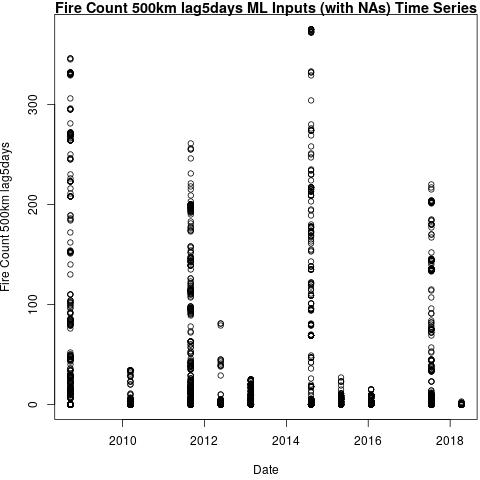
\includegraphics[width=0.77\textwidth]{Code_Outputs/Report_ML_input_PM25_Step4_part_e_de_duplicated_aves_compiled_2019-05-18wNAs_Fire_Count_500km_lag5daysvDate.jpg} 
\caption{\label{fig:Report_ML_input_PM25_Step4_part_e_de_duplicated_aves_compiled_2019-05-18wNAsFire_Count_500km_lag5daysvDate}ML Inputs (with NAs) Time Series} 
\end{figure} 
 

\begin{figure} 
\centering  
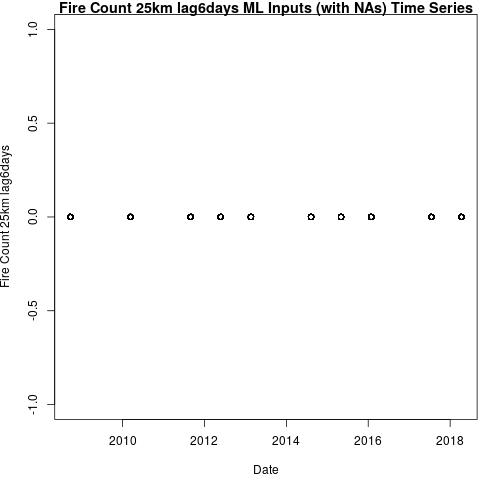
\includegraphics[width=0.77\textwidth]{Code_Outputs/Report_ML_input_PM25_Step4_part_e_de_duplicated_aves_compiled_2019-05-18wNAs_Fire_Count_25km_lag6daysvDate.jpg} 
\caption{\label{fig:Report_ML_input_PM25_Step4_part_e_de_duplicated_aves_compiled_2019-05-18wNAsFire_Count_25km_lag6daysvDate}ML Inputs (with NAs) Time Series} 
\end{figure} 
 

\begin{figure} 
\centering  
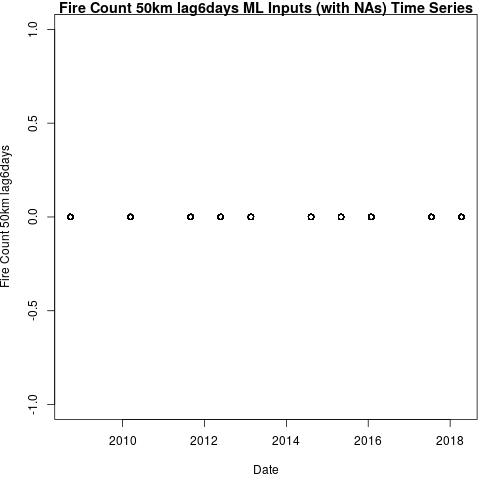
\includegraphics[width=0.77\textwidth]{Code_Outputs/Report_ML_input_PM25_Step4_part_e_de_duplicated_aves_compiled_2019-05-18wNAs_Fire_Count_50km_lag6daysvDate.jpg} 
\caption{\label{fig:Report_ML_input_PM25_Step4_part_e_de_duplicated_aves_compiled_2019-05-18wNAsFire_Count_50km_lag6daysvDate}ML Inputs (with NAs) Time Series} 
\end{figure} 
 

\begin{figure} 
\centering  
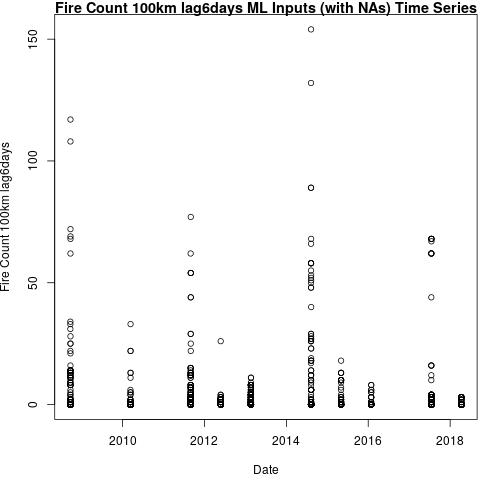
\includegraphics[width=0.77\textwidth]{Code_Outputs/Report_ML_input_PM25_Step4_part_e_de_duplicated_aves_compiled_2019-05-18wNAs_Fire_Count_100km_lag6daysvDate.jpg} 
\caption{\label{fig:Report_ML_input_PM25_Step4_part_e_de_duplicated_aves_compiled_2019-05-18wNAsFire_Count_100km_lag6daysvDate}ML Inputs (with NAs) Time Series} 
\end{figure} 
 

\begin{figure} 
\centering  
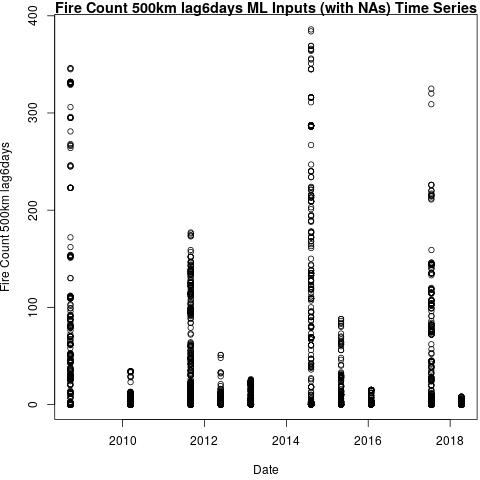
\includegraphics[width=0.77\textwidth]{Code_Outputs/Report_ML_input_PM25_Step4_part_e_de_duplicated_aves_compiled_2019-05-18wNAs_Fire_Count_500km_lag6daysvDate.jpg} 
\caption{\label{fig:Report_ML_input_PM25_Step4_part_e_de_duplicated_aves_compiled_2019-05-18wNAsFire_Count_500km_lag6daysvDate}ML Inputs (with NAs) Time Series} 
\end{figure} 
 

\begin{figure} 
\centering  
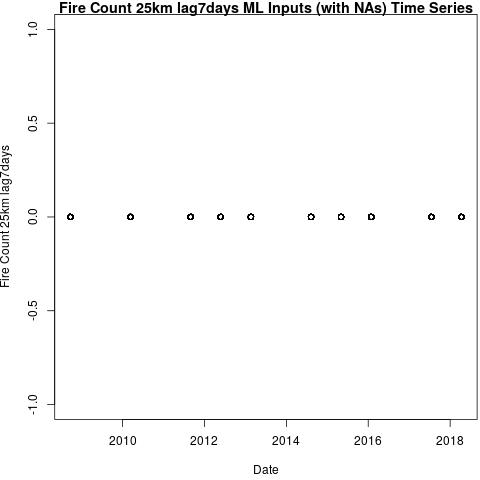
\includegraphics[width=0.77\textwidth]{Code_Outputs/Report_ML_input_PM25_Step4_part_e_de_duplicated_aves_compiled_2019-05-18wNAs_Fire_Count_25km_lag7daysvDate.jpg} 
\caption{\label{fig:Report_ML_input_PM25_Step4_part_e_de_duplicated_aves_compiled_2019-05-18wNAsFire_Count_25km_lag7daysvDate}ML Inputs (with NAs) Time Series} 
\end{figure} 
 

\begin{figure} 
\centering  
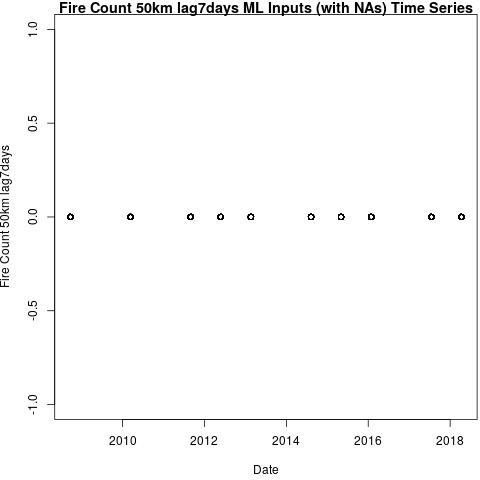
\includegraphics[width=0.77\textwidth]{Code_Outputs/Report_ML_input_PM25_Step4_part_e_de_duplicated_aves_compiled_2019-05-18wNAs_Fire_Count_50km_lag7daysvDate.jpg} 
\caption{\label{fig:Report_ML_input_PM25_Step4_part_e_de_duplicated_aves_compiled_2019-05-18wNAsFire_Count_50km_lag7daysvDate}ML Inputs (with NAs) Time Series} 
\end{figure} 
 

\begin{figure} 
\centering  
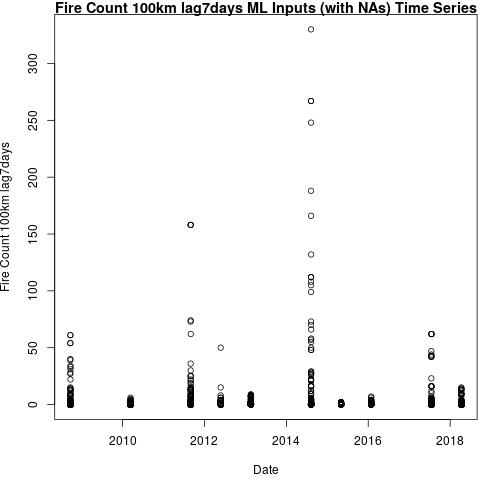
\includegraphics[width=0.77\textwidth]{Code_Outputs/Report_ML_input_PM25_Step4_part_e_de_duplicated_aves_compiled_2019-05-18wNAs_Fire_Count_100km_lag7daysvDate.jpg} 
\caption{\label{fig:Report_ML_input_PM25_Step4_part_e_de_duplicated_aves_compiled_2019-05-18wNAsFire_Count_100km_lag7daysvDate}ML Inputs (with NAs) Time Series} 
\end{figure} 
 

\begin{figure} 
\centering  
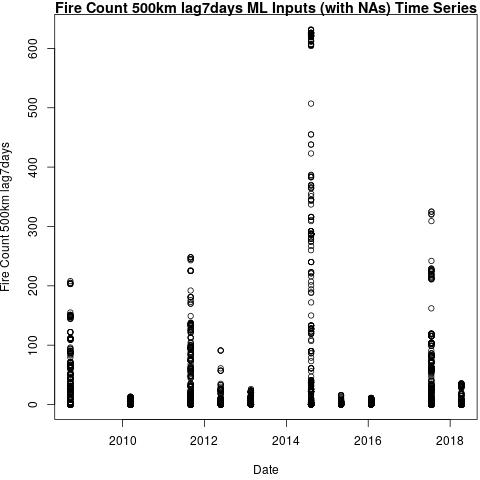
\includegraphics[width=0.77\textwidth]{Code_Outputs/Report_ML_input_PM25_Step4_part_e_de_duplicated_aves_compiled_2019-05-18wNAs_Fire_Count_500km_lag7daysvDate.jpg} 
\caption{\label{fig:Report_ML_input_PM25_Step4_part_e_de_duplicated_aves_compiled_2019-05-18wNAsFire_Count_500km_lag7daysvDate}ML Inputs (with NAs) Time Series} 
\end{figure} 
 

\clearpage 

\begin{figure} 
\centering  
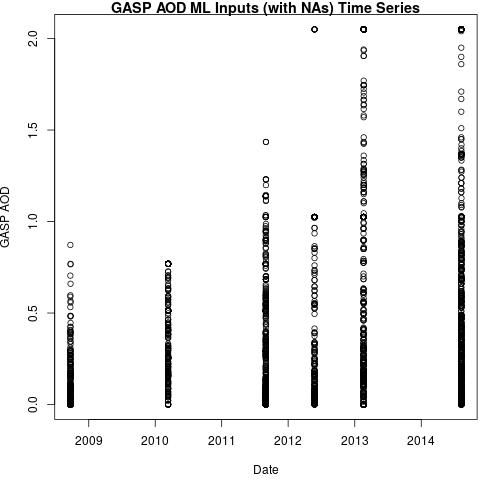
\includegraphics[width=0.77\textwidth]{Code_Outputs/Report_ML_input_PM25_Step4_part_e_de_duplicated_aves_compiled_2019-05-18wNAs_GASP_AODvDate.jpg} 
\caption{\label{fig:Report_ML_input_PM25_Step4_part_e_de_duplicated_aves_compiled_2019-05-18wNAsGASP_AODvDate}ML Inputs (with NAs) Time Series} 
\end{figure} 
 

\begin{figure} 
\centering  
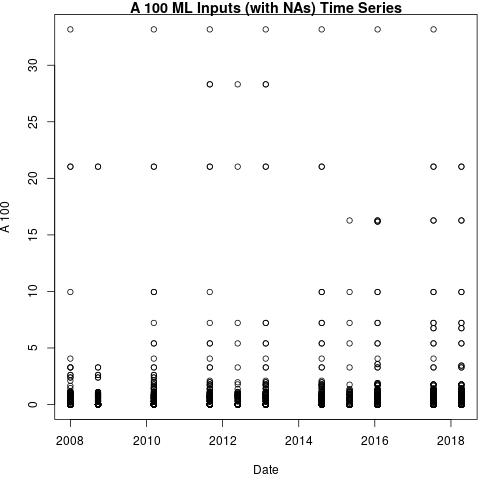
\includegraphics[width=0.77\textwidth]{Code_Outputs/Report_ML_input_PM25_Step4_part_e_de_duplicated_aves_compiled_2019-05-18wNAs_A_100vDate.jpg} 
\caption{\label{fig:Report_ML_input_PM25_Step4_part_e_de_duplicated_aves_compiled_2019-05-18wNAsA_100vDate}ML Inputs (with NAs) Time Series} 
\end{figure} 
 

\begin{figure} 
\centering  
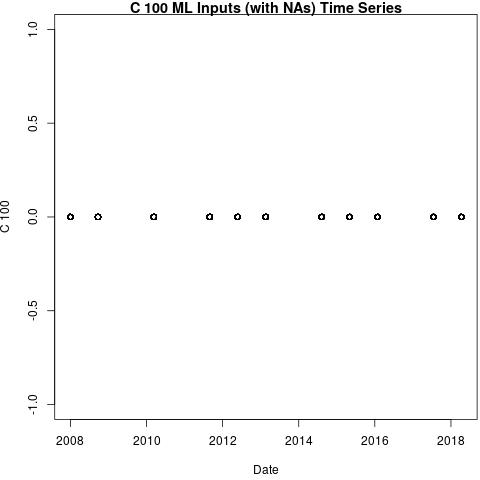
\includegraphics[width=0.77\textwidth]{Code_Outputs/Report_ML_input_PM25_Step4_part_e_de_duplicated_aves_compiled_2019-05-18wNAs_C_100vDate.jpg} 
\caption{\label{fig:Report_ML_input_PM25_Step4_part_e_de_duplicated_aves_compiled_2019-05-18wNAsC_100vDate}ML Inputs (with NAs) Time Series} 
\end{figure} 
 

\begin{figure} 
\centering  
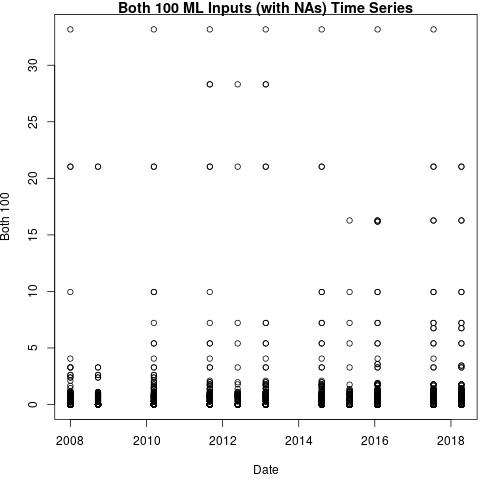
\includegraphics[width=0.77\textwidth]{Code_Outputs/Report_ML_input_PM25_Step4_part_e_de_duplicated_aves_compiled_2019-05-18wNAs_Both_100vDate.jpg} 
\caption{\label{fig:Report_ML_input_PM25_Step4_part_e_de_duplicated_aves_compiled_2019-05-18wNAsBoth_100vDate}ML Inputs (with NAs) Time Series} 
\end{figure} 
 

\begin{figure} 
\centering  
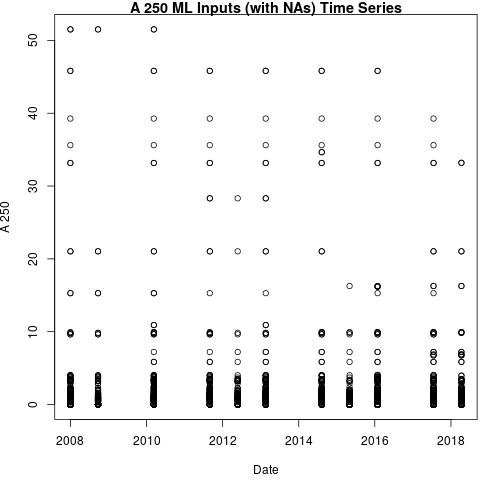
\includegraphics[width=0.77\textwidth]{Code_Outputs/Report_ML_input_PM25_Step4_part_e_de_duplicated_aves_compiled_2019-05-18wNAs_A_250vDate.jpg} 
\caption{\label{fig:Report_ML_input_PM25_Step4_part_e_de_duplicated_aves_compiled_2019-05-18wNAsA_250vDate}ML Inputs (with NAs) Time Series} 
\end{figure} 
 

\begin{figure} 
\centering  
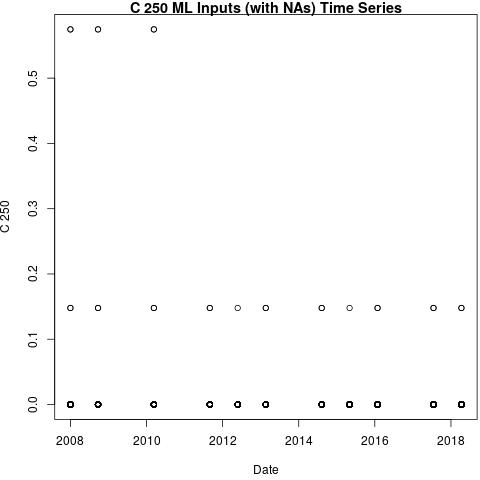
\includegraphics[width=0.77\textwidth]{Code_Outputs/Report_ML_input_PM25_Step4_part_e_de_duplicated_aves_compiled_2019-05-18wNAs_C_250vDate.jpg} 
\caption{\label{fig:Report_ML_input_PM25_Step4_part_e_de_duplicated_aves_compiled_2019-05-18wNAsC_250vDate}ML Inputs (with NAs) Time Series} 
\end{figure} 
 

\begin{figure} 
\centering  
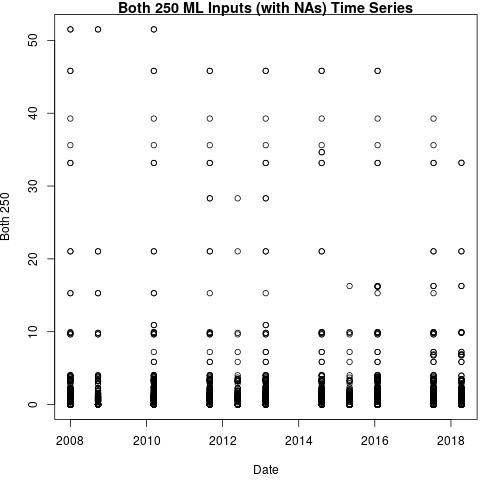
\includegraphics[width=0.77\textwidth]{Code_Outputs/Report_ML_input_PM25_Step4_part_e_de_duplicated_aves_compiled_2019-05-18wNAs_Both_250vDate.jpg} 
\caption{\label{fig:Report_ML_input_PM25_Step4_part_e_de_duplicated_aves_compiled_2019-05-18wNAsBoth_250vDate}ML Inputs (with NAs) Time Series} 
\end{figure} 
 

\begin{figure} 
\centering  
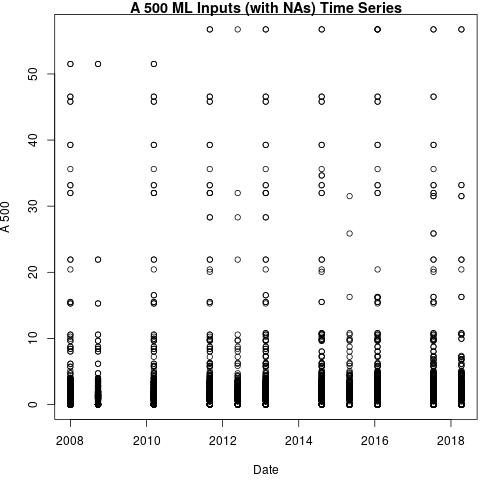
\includegraphics[width=0.77\textwidth]{Code_Outputs/Report_ML_input_PM25_Step4_part_e_de_duplicated_aves_compiled_2019-05-18wNAs_A_500vDate.jpg} 
\caption{\label{fig:Report_ML_input_PM25_Step4_part_e_de_duplicated_aves_compiled_2019-05-18wNAsA_500vDate}ML Inputs (with NAs) Time Series} 
\end{figure} 
 

\begin{figure} 
\centering  
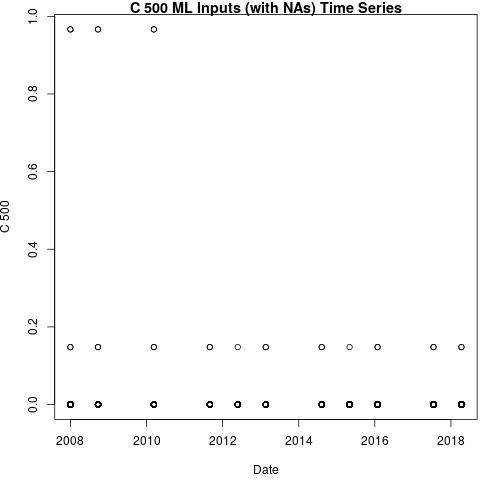
\includegraphics[width=0.77\textwidth]{Code_Outputs/Report_ML_input_PM25_Step4_part_e_de_duplicated_aves_compiled_2019-05-18wNAs_C_500vDate.jpg} 
\caption{\label{fig:Report_ML_input_PM25_Step4_part_e_de_duplicated_aves_compiled_2019-05-18wNAsC_500vDate}ML Inputs (with NAs) Time Series} 
\end{figure} 
 

\begin{figure} 
\centering  
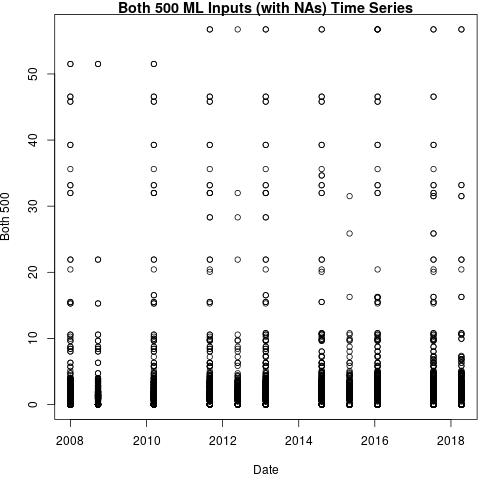
\includegraphics[width=0.77\textwidth]{Code_Outputs/Report_ML_input_PM25_Step4_part_e_de_duplicated_aves_compiled_2019-05-18wNAs_Both_500vDate.jpg} 
\caption{\label{fig:Report_ML_input_PM25_Step4_part_e_de_duplicated_aves_compiled_2019-05-18wNAsBoth_500vDate}ML Inputs (with NAs) Time Series} 
\end{figure} 
 

\clearpage 

\begin{figure} 
\centering  
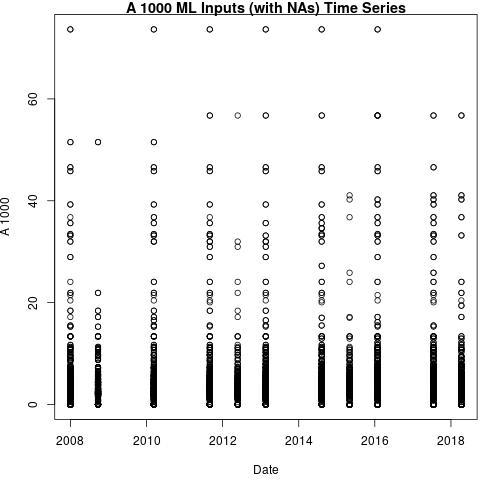
\includegraphics[width=0.77\textwidth]{Code_Outputs/Report_ML_input_PM25_Step4_part_e_de_duplicated_aves_compiled_2019-05-18wNAs_A_1000vDate.jpg} 
\caption{\label{fig:Report_ML_input_PM25_Step4_part_e_de_duplicated_aves_compiled_2019-05-18wNAsA_1000vDate}ML Inputs (with NAs) Time Series} 
\end{figure} 
 

\begin{figure} 
\centering  
\includegraphics[width=0.77\textwidth]{Code_Outputs/Report_ML_input_PM25_Step4_part_e_de_duplicated_aves_compiled_2019-05-18wNAs_Both_1000vDate.jpg} 
\caption{\label{fig:Report_ML_input_PM25_Step4_part_e_de_duplicated_aves_compiled_2019-05-18wNAsBoth_1000vDate}ML Inputs (with NAs) Time Series} 
\end{figure} 
 

\begin{figure} 
\centering  
\includegraphics[width=0.77\textwidth]{Code_Outputs/Report_ML_input_PM25_Step4_part_e_de_duplicated_aves_compiled_2019-05-18wNAs_elevationvDate.jpg} 
\caption{\label{fig:Report_ML_input_PM25_Step4_part_e_de_duplicated_aves_compiled_2019-05-18wNAselevationvDate}ML Inputs (with NAs) Time Series} 
\end{figure} 
 

\begin{figure} 
\centering  
\includegraphics[width=0.77\textwidth]{Code_Outputs/Report_ML_input_PM25_Step4_part_e_de_duplicated_aves_compiled_2019-05-18wNAs_HPBLsurfacevDate.jpg} 
\caption{\label{fig:Report_ML_input_PM25_Step4_part_e_de_duplicated_aves_compiled_2019-05-18wNAsHPBLsurfacevDate}ML Inputs (with NAs) Time Series} 
\end{figure} 
 

\begin{figure} 
\centering  
\includegraphics[width=0.77\textwidth]{Code_Outputs/Report_ML_input_PM25_Step4_part_e_de_duplicated_aves_compiled_2019-05-18wNAs_TMP2mabovegroundvDate.jpg} 
\caption{\label{fig:Report_ML_input_PM25_Step4_part_e_de_duplicated_aves_compiled_2019-05-18wNAsTMP2mabovegroundvDate}ML Inputs (with NAs) Time Series} 
\end{figure} 
 

\begin{figure} 
\centering  
\includegraphics[width=0.77\textwidth]{Code_Outputs/Report_ML_input_PM25_Step4_part_e_de_duplicated_aves_compiled_2019-05-18wNAs_RH2mabovegroundvDate.jpg} 
\caption{\label{fig:Report_ML_input_PM25_Step4_part_e_de_duplicated_aves_compiled_2019-05-18wNAsRH2mabovegroundvDate}ML Inputs (with NAs) Time Series} 
\end{figure} 
 

\begin{figure} 
\centering  
\includegraphics[width=0.77\textwidth]{Code_Outputs/Report_ML_input_PM25_Step4_part_e_de_duplicated_aves_compiled_2019-05-18wNAs_DPT2mabovegroundvDate.jpg} 
\caption{\label{fig:Report_ML_input_PM25_Step4_part_e_de_duplicated_aves_compiled_2019-05-18wNAsDPT2mabovegroundvDate}ML Inputs (with NAs) Time Series} 
\end{figure} 
 

\begin{figure} 
\centering  
\includegraphics[width=0.77\textwidth]{Code_Outputs/Report_ML_input_PM25_Step4_part_e_de_duplicated_aves_compiled_2019-05-18wNAs_APCPsurfacevDate.jpg} 
\caption{\label{fig:Report_ML_input_PM25_Step4_part_e_de_duplicated_aves_compiled_2019-05-18wNAsAPCPsurfacevDate}ML Inputs (with NAs) Time Series} 
\end{figure} 
 

\begin{figure} 
\centering  
\includegraphics[width=0.77\textwidth]{Code_Outputs/Report_ML_input_PM25_Step4_part_e_de_duplicated_aves_compiled_2019-05-18wNAs_WEASDsurfacevDate.jpg} 
\caption{\label{fig:Report_ML_input_PM25_Step4_part_e_de_duplicated_aves_compiled_2019-05-18wNAsWEASDsurfacevDate}ML Inputs (with NAs) Time Series} 
\end{figure} 
 

\begin{figure} 
\centering  
\includegraphics[width=0.77\textwidth]{Code_Outputs/Report_ML_input_PM25_Step4_part_e_de_duplicated_aves_compiled_2019-05-18wNAs_SNOWCsurfacevDate.jpg} 
\caption{\label{fig:Report_ML_input_PM25_Step4_part_e_de_duplicated_aves_compiled_2019-05-18wNAsSNOWCsurfacevDate}ML Inputs (with NAs) Time Series} 
\end{figure} 
 

\clearpage 

\begin{figure} 
\centering  
\includegraphics[width=0.77\textwidth]{Code_Outputs/Report_ML_input_PM25_Step4_part_e_de_duplicated_aves_compiled_2019-05-18wNAs_UGRD10mabovegroundvDate.jpg} 
\caption{\label{fig:Report_ML_input_PM25_Step4_part_e_de_duplicated_aves_compiled_2019-05-18wNAsUGRD10mabovegroundvDate}ML Inputs (with NAs) Time Series} 
\end{figure} 
 

\begin{figure} 
\centering  
\includegraphics[width=0.77\textwidth]{Code_Outputs/Report_ML_input_PM25_Step4_part_e_de_duplicated_aves_compiled_2019-05-18wNAs_VGRD10mabovegroundvDate.jpg} 
\caption{\label{fig:Report_ML_input_PM25_Step4_part_e_de_duplicated_aves_compiled_2019-05-18wNAsVGRD10mabovegroundvDate}ML Inputs (with NAs) Time Series} 
\end{figure} 
 

\begin{figure} 
\centering  
\includegraphics[width=0.77\textwidth]{Code_Outputs/Report_ML_input_PM25_Step4_part_e_de_duplicated_aves_compiled_2019-05-18wNAs_PRMSLmeansealevelvDate.jpg} 
\caption{\label{fig:Report_ML_input_PM25_Step4_part_e_de_duplicated_aves_compiled_2019-05-18wNAsPRMSLmeansealevelvDate}ML Inputs (with NAs) Time Series} 
\end{figure} 
 

\begin{figure} 
\centering  
\includegraphics[width=0.77\textwidth]{Code_Outputs/Report_ML_input_PM25_Step4_part_e_de_duplicated_aves_compiled_2019-05-18wNAs_PRESsurfacevDate.jpg} 
\caption{\label{fig:Report_ML_input_PM25_Step4_part_e_de_duplicated_aves_compiled_2019-05-18wNAsPRESsurfacevDate}ML Inputs (with NAs) Time Series} 
\end{figure} 
 

\begin{figure} 
\centering  
\includegraphics[width=0.77\textwidth]{Code_Outputs/Report_ML_input_PM25_Step4_part_e_de_duplicated_aves_compiled_2019-05-18wNAs_DZDT850mbvDate.jpg} 
\caption{\label{fig:Report_ML_input_PM25_Step4_part_e_de_duplicated_aves_compiled_2019-05-18wNAsDZDT850mbvDate}ML Inputs (with NAs) Time Series} 
\end{figure} 
 

\begin{figure} 
\centering  
\includegraphics[width=0.77\textwidth]{Code_Outputs/Report_ML_input_PM25_Step4_part_e_de_duplicated_aves_compiled_2019-05-18wNAs_DZDT700mbvDate.jpg} 
\caption{\label{fig:Report_ML_input_PM25_Step4_part_e_de_duplicated_aves_compiled_2019-05-18wNAsDZDT700mbvDate}ML Inputs (with NAs) Time Series} 
\end{figure} 
 

\begin{figure} 
\centering  
\includegraphics[width=0.77\textwidth]{Code_Outputs/Report_ML_input_PM25_Step4_part_e_de_duplicated_aves_compiled_2019-05-18wNAs_NLCD_1km_percent_urban_buffervDate.jpg} 
\caption{\label{fig:Report_ML_input_PM25_Step4_part_e_de_duplicated_aves_compiled_2019-05-18wNAsNLCD_1km_percent_urban_buffervDate}ML Inputs (with NAs) Time Series} 
\end{figure} 
 

\begin{figure} 
\centering  
\includegraphics[width=0.77\textwidth]{Code_Outputs/Report_ML_input_PM25_Step4_part_e_de_duplicated_aves_compiled_2019-05-18wNAs_NLCD_5km_percent_urban_buffervDate.jpg} 
\caption{\label{fig:Report_ML_input_PM25_Step4_part_e_de_duplicated_aves_compiled_2019-05-18wNAsNLCD_5km_percent_urban_buffervDate}ML Inputs (with NAs) Time Series} 
\end{figure} 
 

\begin{figure} 
\centering  
\includegraphics[width=0.77\textwidth]{Code_Outputs/Report_ML_input_PM25_Step4_part_e_de_duplicated_aves_compiled_2019-05-18wNAs_NLCD_10km_percent_urban_buffervDate.jpg} 
\caption{\label{fig:Report_ML_input_PM25_Step4_part_e_de_duplicated_aves_compiled_2019-05-18wNAsNLCD_10km_percent_urban_buffervDate}ML Inputs (with NAs) Time Series} 
\end{figure} 
 

\begin{figure} 
\centering  
\includegraphics[width=0.77\textwidth]{Code_Outputs/Report_ML_input_PM25_Step4_part_e_de_duplicated_aves_compiled_2019-05-18wNAs_ndvivDate.jpg} 
\caption{\label{fig:Report_ML_input_PM25_Step4_part_e_de_duplicated_aves_compiled_2019-05-18wNAsndvivDate}ML Inputs (with NAs) Time Series} 
\end{figure} 
 

\clearpage 

\begin{figure} 
\centering  
\includegraphics[width=0.77\textwidth]{Code_Outputs/Report_ML_input_PM25_Step4_part_e_de_duplicated_aves_compiled_2019-05-18wNAs_DayOfWeekvDate.jpg} 
\caption{\label{fig:Report_ML_input_PM25_Step4_part_e_de_duplicated_aves_compiled_2019-05-18wNAsDayOfWeekvDate}ML Inputs (with NAs) Time Series} 
\end{figure} 
 

\begin{figure} 
\centering  
\includegraphics[width=0.77\textwidth]{Code_Outputs/Report_ML_input_PM25_Step4_part_e_de_duplicated_aves_compiled_2019-05-18wNAs_WintervDate.jpg} 
\caption{\label{fig:Report_ML_input_PM25_Step4_part_e_de_duplicated_aves_compiled_2019-05-18wNAsWintervDate}ML Inputs (with NAs) Time Series} 
\end{figure} 
 

\begin{figure} 
\centering  
\includegraphics[width=0.77\textwidth]{Code_Outputs/Report_ML_input_PM25_Step4_part_e_de_duplicated_aves_compiled_2019-05-18wNAs_SpringvDate.jpg} 
\caption{\label{fig:Report_ML_input_PM25_Step4_part_e_de_duplicated_aves_compiled_2019-05-18wNAsSpringvDate}ML Inputs (with NAs) Time Series} 
\end{figure} 
 

\begin{figure} 
\centering  
\includegraphics[width=0.77\textwidth]{Code_Outputs/Report_ML_input_PM25_Step4_part_e_de_duplicated_aves_compiled_2019-05-18wNAs_SummervDate.jpg} 
\caption{\label{fig:Report_ML_input_PM25_Step4_part_e_de_duplicated_aves_compiled_2019-05-18wNAsSummervDate}ML Inputs (with NAs) Time Series} 
\end{figure} 
 

\begin{figure} 
\centering  
\includegraphics[width=0.77\textwidth]{Code_Outputs/Report_ML_input_PM25_Step4_part_e_de_duplicated_aves_compiled_2019-05-18wNAs_FallvDate.jpg} 
\caption{\label{fig:Report_ML_input_PM25_Step4_part_e_de_duplicated_aves_compiled_2019-05-18wNAsFallvDate}ML Inputs (with NAs) Time Series} 
\end{figure} 
 
 

% PM2.5 vs predictor for each predictor variable 

\subsection{ML Inputs (with NAs) Plot against PM2.5 Obs Images} 
 

\begin{figure} 
\centering  
\includegraphics[width=0.77\textwidth]{Code_Outputs/Report_ML_input_PM25_Step4_part_e_de_duplicated_aves_compiled_2019-05-18wNAs_PM25_ObsvPM25_Obs.jpg} 
\caption{\label{fig:Report_ML_input_PM25_Step4_part_e_de_duplicated_aves_compiled_2019-05-18wNAsPM25_ObsvPM25_Obs}ML Inputs (with NAs) Plot against PM2.5 Obs} 
\end{figure} 
 

\begin{figure} 
\centering  
\includegraphics[width=0.77\textwidth]{Code_Outputs/Report_ML_input_PM25_Step4_part_e_de_duplicated_aves_compiled_2019-05-18wNAs_GASP_AODvPM25_Obs.jpg} 
\caption{\label{fig:Report_ML_input_PM25_Step4_part_e_de_duplicated_aves_compiled_2019-05-18wNAsGASP_AODvPM25_Obs}ML Inputs (with NAs) Plot against PM2.5 Obs} 
\end{figure} 
 

\begin{figure} 
\centering  
\includegraphics[width=0.77\textwidth]{Code_Outputs/Report_ML_input_PM25_Step4_part_e_de_duplicated_aves_compiled_2019-05-18wNAs_MAIAC_AODvPM25_Obs.jpg} 
\caption{\label{fig:Report_ML_input_PM25_Step4_part_e_de_duplicated_aves_compiled_2019-05-18wNAsMAIAC_AODvPM25_Obs}ML Inputs (with NAs) Plot against PM2.5 Obs} 
\end{figure} 
 

\begin{figure} 
\centering  
\includegraphics[width=0.77\textwidth]{Code_Outputs/Report_ML_input_PM25_Step4_part_e_de_duplicated_aves_compiled_2019-05-18wNAs_HPBLsurfacevPM25_Obs.jpg} 
\caption{\label{fig:Report_ML_input_PM25_Step4_part_e_de_duplicated_aves_compiled_2019-05-18wNAsHPBLsurfacevPM25_Obs}ML Inputs (with NAs) Plot against PM2.5 Obs} 
\end{figure} 
 

\begin{figure} 
\centering  
\includegraphics[width=0.77\textwidth]{Code_Outputs/Report_ML_input_PM25_Step4_part_e_de_duplicated_aves_compiled_2019-05-18wNAs_TMP2mabovegroundvPM25_Obs.jpg} 
\caption{\label{fig:Report_ML_input_PM25_Step4_part_e_de_duplicated_aves_compiled_2019-05-18wNAsTMP2mabovegroundvPM25_Obs}ML Inputs (with NAs) Plot against PM2.5 Obs} 
\end{figure} 
 

\begin{figure} 
\centering  
\includegraphics[width=0.77\textwidth]{Code_Outputs/Report_ML_input_PM25_Step4_part_e_de_duplicated_aves_compiled_2019-05-18wNAs_RH2mabovegroundvPM25_Obs.jpg} 
\caption{\label{fig:Report_ML_input_PM25_Step4_part_e_de_duplicated_aves_compiled_2019-05-18wNAsRH2mabovegroundvPM25_Obs}ML Inputs (with NAs) Plot against PM2.5 Obs} 
\end{figure} 
 

\begin{figure} 
\centering  
\includegraphics[width=0.77\textwidth]{Code_Outputs/Report_ML_input_PM25_Step4_part_e_de_duplicated_aves_compiled_2019-05-18wNAs_DPT2mabovegroundvPM25_Obs.jpg} 
\caption{\label{fig:Report_ML_input_PM25_Step4_part_e_de_duplicated_aves_compiled_2019-05-18wNAsDPT2mabovegroundvPM25_Obs}ML Inputs (with NAs) Plot against PM2.5 Obs} 
\end{figure} 
 

\begin{figure} 
\centering  
\includegraphics[width=0.77\textwidth]{Code_Outputs/Report_ML_input_PM25_Step4_part_e_de_duplicated_aves_compiled_2019-05-18wNAs_APCPsurfacevPM25_Obs.jpg} 
\caption{\label{fig:Report_ML_input_PM25_Step4_part_e_de_duplicated_aves_compiled_2019-05-18wNAsAPCPsurfacevPM25_Obs}ML Inputs (with NAs) Plot against PM2.5 Obs} 
\end{figure} 
 

\begin{figure} 
\centering  
\includegraphics[width=0.77\textwidth]{Code_Outputs/Report_ML_input_PM25_Step4_part_e_de_duplicated_aves_compiled_2019-05-18wNAs_WEASDsurfacevPM25_Obs.jpg} 
\caption{\label{fig:Report_ML_input_PM25_Step4_part_e_de_duplicated_aves_compiled_2019-05-18wNAsWEASDsurfacevPM25_Obs}ML Inputs (with NAs) Plot against PM2.5 Obs} 
\end{figure} 
 

\clearpage 

\begin{figure} 
\centering  
\includegraphics[width=0.77\textwidth]{Code_Outputs/Report_ML_input_PM25_Step4_part_e_de_duplicated_aves_compiled_2019-05-18wNAs_SNOWCsurfacevPM25_Obs.jpg} 
\caption{\label{fig:Report_ML_input_PM25_Step4_part_e_de_duplicated_aves_compiled_2019-05-18wNAsSNOWCsurfacevPM25_Obs}ML Inputs (with NAs) Plot against PM2.5 Obs} 
\end{figure} 
 

\begin{figure} 
\centering  
\includegraphics[width=0.77\textwidth]{Code_Outputs/Report_ML_input_PM25_Step4_part_e_de_duplicated_aves_compiled_2019-05-18wNAs_UGRD10mabovegroundvPM25_Obs.jpg} 
\caption{\label{fig:Report_ML_input_PM25_Step4_part_e_de_duplicated_aves_compiled_2019-05-18wNAsUGRD10mabovegroundvPM25_Obs}ML Inputs (with NAs) Plot against PM2.5 Obs} 
\end{figure} 
 

\begin{figure} 
\centering  
\includegraphics[width=0.77\textwidth]{Code_Outputs/Report_ML_input_PM25_Step4_part_e_de_duplicated_aves_compiled_2019-05-18wNAs_VGRD10mabovegroundvPM25_Obs.jpg} 
\caption{\label{fig:Report_ML_input_PM25_Step4_part_e_de_duplicated_aves_compiled_2019-05-18wNAsVGRD10mabovegroundvPM25_Obs}ML Inputs (with NAs) Plot against PM2.5 Obs} 
\end{figure} 
 

\begin{figure} 
\centering  
\includegraphics[width=0.77\textwidth]{Code_Outputs/Report_ML_input_PM25_Step4_part_e_de_duplicated_aves_compiled_2019-05-18wNAs_PRMSLmeansealevelvPM25_Obs.jpg} 
\caption{\label{fig:Report_ML_input_PM25_Step4_part_e_de_duplicated_aves_compiled_2019-05-18wNAsPRMSLmeansealevelvPM25_Obs}ML Inputs (with NAs) Plot against PM2.5 Obs} 
\end{figure} 
 

\begin{figure} 
\centering  
\includegraphics[width=0.77\textwidth]{Code_Outputs/Report_ML_input_PM25_Step4_part_e_de_duplicated_aves_compiled_2019-05-18wNAs_PRESsurfacevPM25_Obs.jpg} 
\caption{\label{fig:Report_ML_input_PM25_Step4_part_e_de_duplicated_aves_compiled_2019-05-18wNAsPRESsurfacevPM25_Obs}ML Inputs (with NAs) Plot against PM2.5 Obs} 
\end{figure} 
 

\begin{figure} 
\centering  
\includegraphics[width=0.77\textwidth]{Code_Outputs/Report_ML_input_PM25_Step4_part_e_de_duplicated_aves_compiled_2019-05-18wNAs_DZDT850mbvPM25_Obs.jpg} 
\caption{\label{fig:Report_ML_input_PM25_Step4_part_e_de_duplicated_aves_compiled_2019-05-18wNAsDZDT850mbvPM25_Obs}ML Inputs (with NAs) Plot against PM2.5 Obs} 
\end{figure} 
 

\begin{figure} 
\centering  
\includegraphics[width=0.77\textwidth]{Code_Outputs/Report_ML_input_PM25_Step4_part_e_de_duplicated_aves_compiled_2019-05-18wNAs_DZDT700mbvPM25_Obs.jpg} 
\caption{\label{fig:Report_ML_input_PM25_Step4_part_e_de_duplicated_aves_compiled_2019-05-18wNAsDZDT700mbvPM25_Obs}ML Inputs (with NAs) Plot against PM2.5 Obs} 
\end{figure} 
 

\begin{figure} 
\centering  
\includegraphics[width=0.77\textwidth]{Code_Outputs/Report_ML_input_PM25_Step4_part_e_de_duplicated_aves_compiled_2019-05-18wNAs_NLCD_1km_percent_urban_buffervPM25_Obs.jpg} 
\caption{\label{fig:Report_ML_input_PM25_Step4_part_e_de_duplicated_aves_compiled_2019-05-18wNAsNLCD_1km_percent_urban_buffervPM25_Obs}ML Inputs (with NAs) Plot against PM2.5 Obs} 
\end{figure} 
 

\begin{figure} 
\centering  
\includegraphics[width=0.77\textwidth]{Code_Outputs/Report_ML_input_PM25_Step4_part_e_de_duplicated_aves_compiled_2019-05-18wNAs_NLCD_5km_percent_urban_buffervPM25_Obs.jpg} 
\caption{\label{fig:Report_ML_input_PM25_Step4_part_e_de_duplicated_aves_compiled_2019-05-18wNAsNLCD_5km_percent_urban_buffervPM25_Obs}ML Inputs (with NAs) Plot against PM2.5 Obs} 
\end{figure} 
 

\begin{figure} 
\centering  
\includegraphics[width=0.77\textwidth]{Code_Outputs/Report_ML_input_PM25_Step4_part_e_de_duplicated_aves_compiled_2019-05-18wNAs_NLCD_10km_percent_urban_buffervPM25_Obs.jpg} 
\caption{\label{fig:Report_ML_input_PM25_Step4_part_e_de_duplicated_aves_compiled_2019-05-18wNAsNLCD_10km_percent_urban_buffervPM25_Obs}ML Inputs (with NAs) Plot against PM2.5 Obs} 
\end{figure} 
 
 

% plot maps of a few specific days - aggregated to county averages 

\clearpage 

\begin{figure} 
\centering  
\includegraphics[width=0.77\textwidth]{Code_Outputs/Report_ML_input_PM25_Step4_part_e_de_duplicated_aves_compiled_2019-05-18wNAs_CountyPM25_ObsMean2012-05-25.jpg} 
\caption{\label{fig:Report_ML_input_PM25_Step4_part_e_de_duplicated_aves_compiled_2019-05-18wNAsCountyPM25_ObsMean2012-05-25}ML Inputs (with NAs) PM2.5 Obs 2012-05-25} 
\end{figure} 
 

\clearpage 

\begin{figure} 
\centering  
\includegraphics[width=0.77\textwidth]{Code_Outputs/Report_ML_input_PM25_Step4_part_e_de_duplicated_aves_compiled_2019-05-18wNAs_CountyPM25_ObsMean2012-05-25.jpg} 
\caption{\label{fig:Report_ML_input_PM25_Step4_part_e_de_duplicated_aves_compiled_2019-05-18wNAsCountyPM25_ObsMean2012-05-25}ML Inputs (with NAs) PM2.5 Obs 2012-05-25} 
\end{figure} 
 

\begin{figure} 
\centering  
\includegraphics[width=0.77\textwidth]{Code_Outputs/Report_ML_input_PM25_Step4_part_e_de_duplicated_aves_compiled_2019-05-18wNAs_CountyPM25_ObsMean2014-08-10.jpg} 
\caption{\label{fig:Report_ML_input_PM25_Step4_part_e_de_duplicated_aves_compiled_2019-05-18wNAsCountyPM25_ObsMean2014-08-10}ML Inputs (with NAs) PM2.5 Obs 2014-08-10} 
\end{figure} 
 

\begin{figure} 
\centering  
\includegraphics[width=0.77\textwidth]{Code_Outputs/Report_ML_input_PM25_Step4_part_e_de_duplicated_aves_compiled_2019-05-18wNAs_CountyPM25_ObsMean2008-01-02.jpg} 
\caption{\label{fig:Report_ML_input_PM25_Step4_part_e_de_duplicated_aves_compiled_2019-05-18wNAsCountyPM25_ObsMean2008-01-02}ML Inputs (with NAs) PM2.5 Obs 2008-01-02} 
\end{figure} 
 

\begin{figure} 
\centering  
\includegraphics[width=0.77\textwidth]{Code_Outputs/Report_ML_input_PM25_Step4_part_e_de_duplicated_aves_compiled_2019-05-18wNAs_CountyPM25_ObsMean2015-05-04.jpg} 
\caption{\label{fig:Report_ML_input_PM25_Step4_part_e_de_duplicated_aves_compiled_2019-05-18wNAsCountyPM25_ObsMean2015-05-04}ML Inputs (with NAs) PM2.5 Obs 2015-05-04} 
\end{figure} 
 

\begin{figure} 
\centering  
\includegraphics[width=0.77\textwidth]{Code_Outputs/Report_ML_input_PM25_Step4_part_e_de_duplicated_aves_compiled_2019-05-18wNAs_CountyPM25_ObsMean2018-04-11.jpg} 
\caption{\label{fig:Report_ML_input_PM25_Step4_part_e_de_duplicated_aves_compiled_2019-05-18wNAsCountyPM25_ObsMean2018-04-11}ML Inputs (with NAs) PM2.5 Obs 2018-04-11} 
\end{figure} 
 

\begin{figure} 
\centering  
\includegraphics[width=0.77\textwidth]{Code_Outputs/Report_ML_input_PM25_Step4_part_e_de_duplicated_aves_compiled_2019-05-18wNAs_CountyPM25_ObsMean2008-09-22.jpg} 
\caption{\label{fig:Report_ML_input_PM25_Step4_part_e_de_duplicated_aves_compiled_2019-05-18wNAsCountyPM25_ObsMean2008-09-22}ML Inputs (with NAs) PM2.5 Obs 2008-09-22} 
\end{figure} 
 

\begin{figure} 
\centering  
\includegraphics[width=0.77\textwidth]{Code_Outputs/Report_ML_input_PM25_Step4_part_e_de_duplicated_aves_compiled_2019-05-18wNAs_CountyFire_Count_100km_lag0daysMean2012-05-25.jpg} 
\caption{\label{fig:Report_ML_input_PM25_Step4_part_e_de_duplicated_aves_compiled_2019-05-18wNAsCountyFire_Count_100km_lag0daysMean2012-05-25}ML Inputs (with NAs) Fire Count 100km lag0days 2012-05-25} 
\end{figure} 
 

\begin{figure} 
\centering  
\includegraphics[width=0.77\textwidth]{Code_Outputs/Report_ML_input_PM25_Step4_part_e_de_duplicated_aves_compiled_2019-05-18wNAs_CountyFire_Count_100km_lag0daysMean2014-08-10.jpg} 
\caption{\label{fig:Report_ML_input_PM25_Step4_part_e_de_duplicated_aves_compiled_2019-05-18wNAsCountyFire_Count_100km_lag0daysMean2014-08-10}ML Inputs (with NAs) Fire Count 100km lag0days 2014-08-10} 
\end{figure} 
 

\begin{figure} 
\centering  
\includegraphics[width=0.77\textwidth]{Code_Outputs/Report_ML_input_PM25_Step4_part_e_de_duplicated_aves_compiled_2019-05-18wNAs_CountyFire_Count_100km_lag0daysMean2008-01-02.jpg} 
\caption{\label{fig:Report_ML_input_PM25_Step4_part_e_de_duplicated_aves_compiled_2019-05-18wNAsCountyFire_Count_100km_lag0daysMean2008-01-02}ML Inputs (with NAs) Fire Count 100km lag0days 2008-01-02} 
\end{figure} 
 

\begin{figure} 
\centering  
\includegraphics[width=0.77\textwidth]{Code_Outputs/Report_ML_input_PM25_Step4_part_e_de_duplicated_aves_compiled_2019-05-18wNAs_CountyFire_Count_100km_lag0daysMean2015-05-04.jpg} 
\caption{\label{fig:Report_ML_input_PM25_Step4_part_e_de_duplicated_aves_compiled_2019-05-18wNAsCountyFire_Count_100km_lag0daysMean2015-05-04}ML Inputs (with NAs) Fire Count 100km lag0days 2015-05-04} 
\end{figure} 
 

\begin{figure} 
\centering  
\includegraphics[width=0.77\textwidth]{Code_Outputs/Report_ML_input_PM25_Step4_part_e_de_duplicated_aves_compiled_2019-05-18wNAs_CountyFire_Count_100km_lag0daysMean2018-04-11.jpg} 
\caption{\label{fig:Report_ML_input_PM25_Step4_part_e_de_duplicated_aves_compiled_2019-05-18wNAsCountyFire_Count_100km_lag0daysMean2018-04-11}ML Inputs (with NAs) Fire Count 100km lag0days 2018-04-11} 
\end{figure} 
 

\begin{figure} 
\centering  
\includegraphics[width=0.77\textwidth]{Code_Outputs/Report_ML_input_PM25_Step4_part_e_de_duplicated_aves_compiled_2019-05-18wNAs_CountyFire_Count_100km_lag0daysMean2008-09-22.jpg} 
\caption{\label{fig:Report_ML_input_PM25_Step4_part_e_de_duplicated_aves_compiled_2019-05-18wNAsCountyFire_Count_100km_lag0daysMean2008-09-22}ML Inputs (with NAs) Fire Count 100km lag0days 2008-09-22} 
\end{figure} 
 

\begin{figure} 
\centering  
\includegraphics[width=0.77\textwidth]{Code_Outputs/Report_ML_input_PM25_Step4_part_e_de_duplicated_aves_compiled_2019-05-18wNAs_CountyFire_Count_500km_lag0daysMean2012-05-25.jpg} 
\caption{\label{fig:Report_ML_input_PM25_Step4_part_e_de_duplicated_aves_compiled_2019-05-18wNAsCountyFire_Count_500km_lag0daysMean2012-05-25}ML Inputs (with NAs) Fire Count 500km lag0days 2012-05-25} 
\end{figure} 
 

\begin{figure} 
\centering  
\includegraphics[width=0.77\textwidth]{Code_Outputs/Report_ML_input_PM25_Step4_part_e_de_duplicated_aves_compiled_2019-05-18wNAs_CountyFire_Count_500km_lag0daysMean2014-08-10.jpg} 
\caption{\label{fig:Report_ML_input_PM25_Step4_part_e_de_duplicated_aves_compiled_2019-05-18wNAsCountyFire_Count_500km_lag0daysMean2014-08-10}ML Inputs (with NAs) Fire Count 500km lag0days 2014-08-10} 
\end{figure} 
 

\clearpage 

\begin{figure} 
\centering  
\includegraphics[width=0.77\textwidth]{Code_Outputs/Report_ML_input_PM25_Step4_part_e_de_duplicated_aves_compiled_2019-05-18wNAs_CountyFire_Count_500km_lag0daysMean2008-01-02.jpg} 
\caption{\label{fig:Report_ML_input_PM25_Step4_part_e_de_duplicated_aves_compiled_2019-05-18wNAsCountyFire_Count_500km_lag0daysMean2008-01-02}ML Inputs (with NAs) Fire Count 500km lag0days 2008-01-02} 
\end{figure} 
 

\begin{figure} 
\centering  
\includegraphics[width=0.77\textwidth]{Code_Outputs/Report_ML_input_PM25_Step4_part_e_de_duplicated_aves_compiled_2019-05-18wNAs_CountyFire_Count_500km_lag0daysMean2015-05-04.jpg} 
\caption{\label{fig:Report_ML_input_PM25_Step4_part_e_de_duplicated_aves_compiled_2019-05-18wNAsCountyFire_Count_500km_lag0daysMean2015-05-04}ML Inputs (with NAs) Fire Count 500km lag0days 2015-05-04} 
\end{figure} 
 

\begin{figure} 
\centering  
\includegraphics[width=0.77\textwidth]{Code_Outputs/Report_ML_input_PM25_Step4_part_e_de_duplicated_aves_compiled_2019-05-18wNAs_CountyFire_Count_500km_lag0daysMean2018-04-11.jpg} 
\caption{\label{fig:Report_ML_input_PM25_Step4_part_e_de_duplicated_aves_compiled_2019-05-18wNAsCountyFire_Count_500km_lag0daysMean2018-04-11}ML Inputs (with NAs) Fire Count 500km lag0days 2018-04-11} 
\end{figure} 
 

\begin{figure} 
\centering  
\includegraphics[width=0.77\textwidth]{Code_Outputs/Report_ML_input_PM25_Step4_part_e_de_duplicated_aves_compiled_2019-05-18wNAs_CountyFire_Count_500km_lag0daysMean2008-09-22.jpg} 
\caption{\label{fig:Report_ML_input_PM25_Step4_part_e_de_duplicated_aves_compiled_2019-05-18wNAsCountyFire_Count_500km_lag0daysMean2008-09-22}ML Inputs (with NAs) Fire Count 500km lag0days 2008-09-22} 
\end{figure} 
 

\begin{figure} 
\centering  
\includegraphics[width=0.77\textwidth]{Code_Outputs/Report_ML_input_PM25_Step4_part_e_de_duplicated_aves_compiled_2019-05-18wNAs_CountyFire_Count_100km_lag1daysMean2012-05-25.jpg} 
\caption{\label{fig:Report_ML_input_PM25_Step4_part_e_de_duplicated_aves_compiled_2019-05-18wNAsCountyFire_Count_100km_lag1daysMean2012-05-25}ML Inputs (with NAs) Fire Count 100km lag1days 2012-05-25} 
\end{figure} 
 

\begin{figure} 
\centering  
\includegraphics[width=0.77\textwidth]{Code_Outputs/Report_ML_input_PM25_Step4_part_e_de_duplicated_aves_compiled_2019-05-18wNAs_CountyFire_Count_100km_lag1daysMean2014-08-10.jpg} 
\caption{\label{fig:Report_ML_input_PM25_Step4_part_e_de_duplicated_aves_compiled_2019-05-18wNAsCountyFire_Count_100km_lag1daysMean2014-08-10}ML Inputs (with NAs) Fire Count 100km lag1days 2014-08-10} 
\end{figure} 
 

\begin{figure} 
\centering  
\includegraphics[width=0.77\textwidth]{Code_Outputs/Report_ML_input_PM25_Step4_part_e_de_duplicated_aves_compiled_2019-05-18wNAs_CountyFire_Count_100km_lag1daysMean2008-01-02.jpg} 
\caption{\label{fig:Report_ML_input_PM25_Step4_part_e_de_duplicated_aves_compiled_2019-05-18wNAsCountyFire_Count_100km_lag1daysMean2008-01-02}ML Inputs (with NAs) Fire Count 100km lag1days 2008-01-02} 
\end{figure} 
 

\begin{figure} 
\centering  
\includegraphics[width=0.77\textwidth]{Code_Outputs/Report_ML_input_PM25_Step4_part_e_de_duplicated_aves_compiled_2019-05-18wNAs_CountyFire_Count_100km_lag1daysMean2015-05-04.jpg} 
\caption{\label{fig:Report_ML_input_PM25_Step4_part_e_de_duplicated_aves_compiled_2019-05-18wNAsCountyFire_Count_100km_lag1daysMean2015-05-04}ML Inputs (with NAs) Fire Count 100km lag1days 2015-05-04} 
\end{figure} 
 

\clearpage 

\begin{figure} 
\centering  
\includegraphics[width=0.77\textwidth]{Code_Outputs/Report_ML_input_PM25_Step4_part_e_de_duplicated_aves_compiled_2019-05-18wNAs_CountyFire_Count_100km_lag1daysMean2018-04-11.jpg} 
\caption{\label{fig:Report_ML_input_PM25_Step4_part_e_de_duplicated_aves_compiled_2019-05-18wNAsCountyFire_Count_100km_lag1daysMean2018-04-11}ML Inputs (with NAs) Fire Count 100km lag1days 2018-04-11} 
\end{figure} 
 

\begin{figure} 
\centering  
\includegraphics[width=0.77\textwidth]{Code_Outputs/Report_ML_input_PM25_Step4_part_e_de_duplicated_aves_compiled_2019-05-18wNAs_CountyFire_Count_100km_lag1daysMean2008-09-22.jpg} 
\caption{\label{fig:Report_ML_input_PM25_Step4_part_e_de_duplicated_aves_compiled_2019-05-18wNAsCountyFire_Count_100km_lag1daysMean2008-09-22}ML Inputs (with NAs) Fire Count 100km lag1days 2008-09-22} 
\end{figure} 
 

\begin{figure} 
\centering  
\includegraphics[width=0.77\textwidth]{Code_Outputs/Report_ML_input_PM25_Step4_part_e_de_duplicated_aves_compiled_2019-05-18wNAs_CountyFire_Count_500km_lag1daysMean2012-05-25.jpg} 
\caption{\label{fig:Report_ML_input_PM25_Step4_part_e_de_duplicated_aves_compiled_2019-05-18wNAsCountyFire_Count_500km_lag1daysMean2012-05-25}ML Inputs (with NAs) Fire Count 500km lag1days 2012-05-25} 
\end{figure} 
 

\begin{figure} 
\centering  
\includegraphics[width=0.77\textwidth]{Code_Outputs/Report_ML_input_PM25_Step4_part_e_de_duplicated_aves_compiled_2019-05-18wNAs_CountyFire_Count_500km_lag1daysMean2014-08-10.jpg} 
\caption{\label{fig:Report_ML_input_PM25_Step4_part_e_de_duplicated_aves_compiled_2019-05-18wNAsCountyFire_Count_500km_lag1daysMean2014-08-10}ML Inputs (with NAs) Fire Count 500km lag1days 2014-08-10} 
\end{figure} 
 

\begin{figure} 
\centering  
\includegraphics[width=0.77\textwidth]{Code_Outputs/Report_ML_input_PM25_Step4_part_e_de_duplicated_aves_compiled_2019-05-18wNAs_CountyFire_Count_500km_lag1daysMean2008-01-02.jpg} 
\caption{\label{fig:Report_ML_input_PM25_Step4_part_e_de_duplicated_aves_compiled_2019-05-18wNAsCountyFire_Count_500km_lag1daysMean2008-01-02}ML Inputs (with NAs) Fire Count 500km lag1days 2008-01-02} 
\end{figure} 
 

\begin{figure} 
\centering  
\includegraphics[width=0.77\textwidth]{Code_Outputs/Report_ML_input_PM25_Step4_part_e_de_duplicated_aves_compiled_2019-05-18wNAs_CountyFire_Count_500km_lag1daysMean2015-05-04.jpg} 
\caption{\label{fig:Report_ML_input_PM25_Step4_part_e_de_duplicated_aves_compiled_2019-05-18wNAsCountyFire_Count_500km_lag1daysMean2015-05-04}ML Inputs (with NAs) Fire Count 500km lag1days 2015-05-04} 
\end{figure} 
 

\begin{figure} 
\centering  
\includegraphics[width=0.77\textwidth]{Code_Outputs/Report_ML_input_PM25_Step4_part_e_de_duplicated_aves_compiled_2019-05-18wNAs_CountyFire_Count_500km_lag1daysMean2018-04-11.jpg} 
\caption{\label{fig:Report_ML_input_PM25_Step4_part_e_de_duplicated_aves_compiled_2019-05-18wNAsCountyFire_Count_500km_lag1daysMean2018-04-11}ML Inputs (with NAs) Fire Count 500km lag1days 2018-04-11} 
\end{figure} 
 

\begin{figure} 
\centering  
\includegraphics[width=0.77\textwidth]{Code_Outputs/Report_ML_input_PM25_Step4_part_e_de_duplicated_aves_compiled_2019-05-18wNAs_CountyFire_Count_500km_lag1daysMean2008-09-22.jpg} 
\caption{\label{fig:Report_ML_input_PM25_Step4_part_e_de_duplicated_aves_compiled_2019-05-18wNAsCountyFire_Count_500km_lag1daysMean2008-09-22}ML Inputs (with NAs) Fire Count 500km lag1days 2008-09-22} 
\end{figure} 
 

\clearpage 

\begin{figure} 
\centering  
\includegraphics[width=0.77\textwidth]{Code_Outputs/Report_ML_input_PM25_Step4_part_e_de_duplicated_aves_compiled_2019-05-18wNAs_CountyFire_Count_100km_lag2daysMean2012-05-25.jpg} 
\caption{\label{fig:Report_ML_input_PM25_Step4_part_e_de_duplicated_aves_compiled_2019-05-18wNAsCountyFire_Count_100km_lag2daysMean2012-05-25}ML Inputs (with NAs) Fire Count 100km lag2days 2012-05-25} 
\end{figure} 
 

\begin{figure} 
\centering  
\includegraphics[width=0.77\textwidth]{Code_Outputs/Report_ML_input_PM25_Step4_part_e_de_duplicated_aves_compiled_2019-05-18wNAs_CountyFire_Count_100km_lag2daysMean2014-08-10.jpg} 
\caption{\label{fig:Report_ML_input_PM25_Step4_part_e_de_duplicated_aves_compiled_2019-05-18wNAsCountyFire_Count_100km_lag2daysMean2014-08-10}ML Inputs (with NAs) Fire Count 100km lag2days 2014-08-10} 
\end{figure} 
 

\begin{figure} 
\centering  
\includegraphics[width=0.77\textwidth]{Code_Outputs/Report_ML_input_PM25_Step4_part_e_de_duplicated_aves_compiled_2019-05-18wNAs_CountyFire_Count_100km_lag2daysMean2015-05-04.jpg} 
\caption{\label{fig:Report_ML_input_PM25_Step4_part_e_de_duplicated_aves_compiled_2019-05-18wNAsCountyFire_Count_100km_lag2daysMean2015-05-04}ML Inputs (with NAs) Fire Count 100km lag2days 2015-05-04} 
\end{figure} 
 

\begin{figure} 
\centering  
\includegraphics[width=0.77\textwidth]{Code_Outputs/Report_ML_input_PM25_Step4_part_e_de_duplicated_aves_compiled_2019-05-18wNAs_CountyFire_Count_100km_lag2daysMean2018-04-11.jpg} 
\caption{\label{fig:Report_ML_input_PM25_Step4_part_e_de_duplicated_aves_compiled_2019-05-18wNAsCountyFire_Count_100km_lag2daysMean2018-04-11}ML Inputs (with NAs) Fire Count 100km lag2days 2018-04-11} 
\end{figure} 
 

\begin{figure} 
\centering  
\includegraphics[width=0.77\textwidth]{Code_Outputs/Report_ML_input_PM25_Step4_part_e_de_duplicated_aves_compiled_2019-05-18wNAs_CountyFire_Count_100km_lag2daysMean2008-09-22.jpg} 
\caption{\label{fig:Report_ML_input_PM25_Step4_part_e_de_duplicated_aves_compiled_2019-05-18wNAsCountyFire_Count_100km_lag2daysMean2008-09-22}ML Inputs (with NAs) Fire Count 100km lag2days 2008-09-22} 
\end{figure} 
 

\begin{figure} 
\centering  
\includegraphics[width=0.77\textwidth]{Code_Outputs/Report_ML_input_PM25_Step4_part_e_de_duplicated_aves_compiled_2019-05-18wNAs_CountyFire_Count_500km_lag2daysMean2012-05-25.jpg} 
\caption{\label{fig:Report_ML_input_PM25_Step4_part_e_de_duplicated_aves_compiled_2019-05-18wNAsCountyFire_Count_500km_lag2daysMean2012-05-25}ML Inputs (with NAs) Fire Count 500km lag2days 2012-05-25} 
\end{figure} 
 

\begin{figure} 
\centering  
\includegraphics[width=0.77\textwidth]{Code_Outputs/Report_ML_input_PM25_Step4_part_e_de_duplicated_aves_compiled_2019-05-18wNAs_CountyFire_Count_500km_lag2daysMean2014-08-10.jpg} 
\caption{\label{fig:Report_ML_input_PM25_Step4_part_e_de_duplicated_aves_compiled_2019-05-18wNAsCountyFire_Count_500km_lag2daysMean2014-08-10}ML Inputs (with NAs) Fire Count 500km lag2days 2014-08-10} 
\end{figure} 
 

\begin{figure} 
\centering  
\includegraphics[width=0.77\textwidth]{Code_Outputs/Report_ML_input_PM25_Step4_part_e_de_duplicated_aves_compiled_2019-05-18wNAs_CountyFire_Count_500km_lag2daysMean2015-05-04.jpg} 
\caption{\label{fig:Report_ML_input_PM25_Step4_part_e_de_duplicated_aves_compiled_2019-05-18wNAsCountyFire_Count_500km_lag2daysMean2015-05-04}ML Inputs (with NAs) Fire Count 500km lag2days 2015-05-04} 
\end{figure} 
 

\clearpage 

\begin{figure} 
\centering  
\includegraphics[width=0.77\textwidth]{Code_Outputs/Report_ML_input_PM25_Step4_part_e_de_duplicated_aves_compiled_2019-05-18wNAs_CountyFire_Count_500km_lag2daysMean2018-04-11.jpg} 
\caption{\label{fig:Report_ML_input_PM25_Step4_part_e_de_duplicated_aves_compiled_2019-05-18wNAsCountyFire_Count_500km_lag2daysMean2018-04-11}ML Inputs (with NAs) Fire Count 500km lag2days 2018-04-11} 
\end{figure} 
 

\begin{figure} 
\centering  
\includegraphics[width=0.77\textwidth]{Code_Outputs/Report_ML_input_PM25_Step4_part_e_de_duplicated_aves_compiled_2019-05-18wNAs_CountyFire_Count_500km_lag2daysMean2008-09-22.jpg} 
\caption{\label{fig:Report_ML_input_PM25_Step4_part_e_de_duplicated_aves_compiled_2019-05-18wNAsCountyFire_Count_500km_lag2daysMean2008-09-22}ML Inputs (with NAs) Fire Count 500km lag2days 2008-09-22} 
\end{figure} 
 

\begin{figure} 
\centering  
\includegraphics[width=0.77\textwidth]{Code_Outputs/Report_ML_input_PM25_Step4_part_e_de_duplicated_aves_compiled_2019-05-18wNAs_CountyFire_Count_100km_lag3daysMean2012-05-25.jpg} 
\caption{\label{fig:Report_ML_input_PM25_Step4_part_e_de_duplicated_aves_compiled_2019-05-18wNAsCountyFire_Count_100km_lag3daysMean2012-05-25}ML Inputs (with NAs) Fire Count 100km lag3days 2012-05-25} 
\end{figure} 
 

\begin{figure} 
\centering  
\includegraphics[width=0.77\textwidth]{Code_Outputs/Report_ML_input_PM25_Step4_part_e_de_duplicated_aves_compiled_2019-05-18wNAs_CountyFire_Count_100km_lag3daysMean2014-08-10.jpg} 
\caption{\label{fig:Report_ML_input_PM25_Step4_part_e_de_duplicated_aves_compiled_2019-05-18wNAsCountyFire_Count_100km_lag3daysMean2014-08-10}ML Inputs (with NAs) Fire Count 100km lag3days 2014-08-10} 
\end{figure} 
 

\begin{figure} 
\centering  
\includegraphics[width=0.77\textwidth]{Code_Outputs/Report_ML_input_PM25_Step4_part_e_de_duplicated_aves_compiled_2019-05-18wNAs_CountyFire_Count_100km_lag3daysMean2015-05-04.jpg} 
\caption{\label{fig:Report_ML_input_PM25_Step4_part_e_de_duplicated_aves_compiled_2019-05-18wNAsCountyFire_Count_100km_lag3daysMean2015-05-04}ML Inputs (with NAs) Fire Count 100km lag3days 2015-05-04} 
\end{figure} 
 

\begin{figure} 
\centering  
\includegraphics[width=0.77\textwidth]{Code_Outputs/Report_ML_input_PM25_Step4_part_e_de_duplicated_aves_compiled_2019-05-18wNAs_CountyFire_Count_100km_lag3daysMean2018-04-11.jpg} 
\caption{\label{fig:Report_ML_input_PM25_Step4_part_e_de_duplicated_aves_compiled_2019-05-18wNAsCountyFire_Count_100km_lag3daysMean2018-04-11}ML Inputs (with NAs) Fire Count 100km lag3days 2018-04-11} 
\end{figure} 
 

\begin{figure} 
\centering  
\includegraphics[width=0.77\textwidth]{Code_Outputs/Report_ML_input_PM25_Step4_part_e_de_duplicated_aves_compiled_2019-05-18wNAs_CountyFire_Count_100km_lag3daysMean2008-09-22.jpg} 
\caption{\label{fig:Report_ML_input_PM25_Step4_part_e_de_duplicated_aves_compiled_2019-05-18wNAsCountyFire_Count_100km_lag3daysMean2008-09-22}ML Inputs (with NAs) Fire Count 100km lag3days 2008-09-22} 
\end{figure} 
 

\clearpage 

\begin{figure} 
\centering  
\includegraphics[width=0.77\textwidth]{Code_Outputs/Report_ML_input_PM25_Step4_part_e_de_duplicated_aves_compiled_2019-05-18wNAs_CountyFire_Count_500km_lag3daysMean2012-05-25.jpg} 
\caption{\label{fig:Report_ML_input_PM25_Step4_part_e_de_duplicated_aves_compiled_2019-05-18wNAsCountyFire_Count_500km_lag3daysMean2012-05-25}ML Inputs (with NAs) Fire Count 500km lag3days 2012-05-25} 
\end{figure} 
 

\begin{figure} 
\centering  
\includegraphics[width=0.77\textwidth]{Code_Outputs/Report_ML_input_PM25_Step4_part_e_de_duplicated_aves_compiled_2019-05-18wNAs_CountyFire_Count_500km_lag3daysMean2014-08-10.jpg} 
\caption{\label{fig:Report_ML_input_PM25_Step4_part_e_de_duplicated_aves_compiled_2019-05-18wNAsCountyFire_Count_500km_lag3daysMean2014-08-10}ML Inputs (with NAs) Fire Count 500km lag3days 2014-08-10} 
\end{figure} 
 

\begin{figure} 
\centering  
\includegraphics[width=0.77\textwidth]{Code_Outputs/Report_ML_input_PM25_Step4_part_e_de_duplicated_aves_compiled_2019-05-18wNAs_CountyFire_Count_500km_lag3daysMean2015-05-04.jpg} 
\caption{\label{fig:Report_ML_input_PM25_Step4_part_e_de_duplicated_aves_compiled_2019-05-18wNAsCountyFire_Count_500km_lag3daysMean2015-05-04}ML Inputs (with NAs) Fire Count 500km lag3days 2015-05-04} 
\end{figure} 
 

\begin{figure} 
\centering  
\includegraphics[width=0.77\textwidth]{Code_Outputs/Report_ML_input_PM25_Step4_part_e_de_duplicated_aves_compiled_2019-05-18wNAs_CountyFire_Count_500km_lag3daysMean2018-04-11.jpg} 
\caption{\label{fig:Report_ML_input_PM25_Step4_part_e_de_duplicated_aves_compiled_2019-05-18wNAsCountyFire_Count_500km_lag3daysMean2018-04-11}ML Inputs (with NAs) Fire Count 500km lag3days 2018-04-11} 
\end{figure} 
 

\begin{figure} 
\centering  
\includegraphics[width=0.77\textwidth]{Code_Outputs/Report_ML_input_PM25_Step4_part_e_de_duplicated_aves_compiled_2019-05-18wNAs_CountyFire_Count_500km_lag3daysMean2008-09-22.jpg} 
\caption{\label{fig:Report_ML_input_PM25_Step4_part_e_de_duplicated_aves_compiled_2019-05-18wNAsCountyFire_Count_500km_lag3daysMean2008-09-22}ML Inputs (with NAs) Fire Count 500km lag3days 2008-09-22} 
\end{figure} 
 

\begin{figure} 
\centering  
\includegraphics[width=0.77\textwidth]{Code_Outputs/Report_ML_input_PM25_Step4_part_e_de_duplicated_aves_compiled_2019-05-18wNAs_CountyFire_Count_100km_lag4daysMean2012-05-25.jpg} 
\caption{\label{fig:Report_ML_input_PM25_Step4_part_e_de_duplicated_aves_compiled_2019-05-18wNAsCountyFire_Count_100km_lag4daysMean2012-05-25}ML Inputs (with NAs) Fire Count 100km lag4days 2012-05-25} 
\end{figure} 
 

\begin{figure} 
\centering  
\includegraphics[width=0.77\textwidth]{Code_Outputs/Report_ML_input_PM25_Step4_part_e_de_duplicated_aves_compiled_2019-05-18wNAs_CountyFire_Count_100km_lag4daysMean2014-08-10.jpg} 
\caption{\label{fig:Report_ML_input_PM25_Step4_part_e_de_duplicated_aves_compiled_2019-05-18wNAsCountyFire_Count_100km_lag4daysMean2014-08-10}ML Inputs (with NAs) Fire Count 100km lag4days 2014-08-10} 
\end{figure} 
 

\begin{figure} 
\centering  
\includegraphics[width=0.77\textwidth]{Code_Outputs/Report_ML_input_PM25_Step4_part_e_de_duplicated_aves_compiled_2019-05-18wNAs_CountyFire_Count_100km_lag4daysMean2015-05-04.jpg} 
\caption{\label{fig:Report_ML_input_PM25_Step4_part_e_de_duplicated_aves_compiled_2019-05-18wNAsCountyFire_Count_100km_lag4daysMean2015-05-04}ML Inputs (with NAs) Fire Count 100km lag4days 2015-05-04} 
\end{figure} 
 

\begin{figure} 
\centering  
\includegraphics[width=0.77\textwidth]{Code_Outputs/Report_ML_input_PM25_Step4_part_e_de_duplicated_aves_compiled_2019-05-18wNAs_CountyFire_Count_100km_lag4daysMean2018-04-11.jpg} 
\caption{\label{fig:Report_ML_input_PM25_Step4_part_e_de_duplicated_aves_compiled_2019-05-18wNAsCountyFire_Count_100km_lag4daysMean2018-04-11}ML Inputs (with NAs) Fire Count 100km lag4days 2018-04-11} 
\end{figure} 
 

\begin{figure} 
\centering  
\includegraphics[width=0.77\textwidth]{Code_Outputs/Report_ML_input_PM25_Step4_part_e_de_duplicated_aves_compiled_2019-05-18wNAs_CountyFire_Count_100km_lag4daysMean2008-09-22.jpg} 
\caption{\label{fig:Report_ML_input_PM25_Step4_part_e_de_duplicated_aves_compiled_2019-05-18wNAsCountyFire_Count_100km_lag4daysMean2008-09-22}ML Inputs (with NAs) Fire Count 100km lag4days 2008-09-22} 
\end{figure} 
 

\begin{figure} 
\centering  
\includegraphics[width=0.77\textwidth]{Code_Outputs/Report_ML_input_PM25_Step4_part_e_de_duplicated_aves_compiled_2019-05-18wNAs_CountyFire_Count_500km_lag4daysMean2012-05-25.jpg} 
\caption{\label{fig:Report_ML_input_PM25_Step4_part_e_de_duplicated_aves_compiled_2019-05-18wNAsCountyFire_Count_500km_lag4daysMean2012-05-25}ML Inputs (with NAs) Fire Count 500km lag4days 2012-05-25} 
\end{figure} 
 

\begin{figure} 
\centering  
\includegraphics[width=0.77\textwidth]{Code_Outputs/Report_ML_input_PM25_Step4_part_e_de_duplicated_aves_compiled_2019-05-18wNAs_CountyFire_Count_500km_lag4daysMean2014-08-10.jpg} 
\caption{\label{fig:Report_ML_input_PM25_Step4_part_e_de_duplicated_aves_compiled_2019-05-18wNAsCountyFire_Count_500km_lag4daysMean2014-08-10}ML Inputs (with NAs) Fire Count 500km lag4days 2014-08-10} 
\end{figure} 
 

\begin{figure} 
\centering  
\includegraphics[width=0.77\textwidth]{Code_Outputs/Report_ML_input_PM25_Step4_part_e_de_duplicated_aves_compiled_2019-05-18wNAs_CountyFire_Count_500km_lag4daysMean2015-05-04.jpg} 
\caption{\label{fig:Report_ML_input_PM25_Step4_part_e_de_duplicated_aves_compiled_2019-05-18wNAsCountyFire_Count_500km_lag4daysMean2015-05-04}ML Inputs (with NAs) Fire Count 500km lag4days 2015-05-04} 
\end{figure} 
 

\begin{figure} 
\centering  
\includegraphics[width=0.77\textwidth]{Code_Outputs/Report_ML_input_PM25_Step4_part_e_de_duplicated_aves_compiled_2019-05-18wNAs_CountyFire_Count_500km_lag4daysMean2018-04-11.jpg} 
\caption{\label{fig:Report_ML_input_PM25_Step4_part_e_de_duplicated_aves_compiled_2019-05-18wNAsCountyFire_Count_500km_lag4daysMean2018-04-11}ML Inputs (with NAs) Fire Count 500km lag4days 2018-04-11} 
\end{figure} 
 

\begin{figure} 
\centering  
\includegraphics[width=0.77\textwidth]{Code_Outputs/Report_ML_input_PM25_Step4_part_e_de_duplicated_aves_compiled_2019-05-18wNAs_CountyFire_Count_500km_lag4daysMean2008-09-22.jpg} 
\caption{\label{fig:Report_ML_input_PM25_Step4_part_e_de_duplicated_aves_compiled_2019-05-18wNAsCountyFire_Count_500km_lag4daysMean2008-09-22}ML Inputs (with NAs) Fire Count 500km lag4days 2008-09-22} 
\end{figure} 
 

\begin{figure} 
\centering  
\includegraphics[width=0.77\textwidth]{Code_Outputs/Report_ML_input_PM25_Step4_part_e_de_duplicated_aves_compiled_2019-05-18wNAs_CountyFire_Count_100km_lag5daysMean2012-05-25.jpg} 
\caption{\label{fig:Report_ML_input_PM25_Step4_part_e_de_duplicated_aves_compiled_2019-05-18wNAsCountyFire_Count_100km_lag5daysMean2012-05-25}ML Inputs (with NAs) Fire Count 100km lag5days 2012-05-25} 
\end{figure} 
 

\begin{figure} 
\centering  
\includegraphics[width=0.77\textwidth]{Code_Outputs/Report_ML_input_PM25_Step4_part_e_de_duplicated_aves_compiled_2019-05-18wNAs_CountyFire_Count_100km_lag5daysMean2014-08-10.jpg} 
\caption{\label{fig:Report_ML_input_PM25_Step4_part_e_de_duplicated_aves_compiled_2019-05-18wNAsCountyFire_Count_100km_lag5daysMean2014-08-10}ML Inputs (with NAs) Fire Count 100km lag5days 2014-08-10} 
\end{figure} 
 

\begin{figure} 
\centering  
\includegraphics[width=0.77\textwidth]{Code_Outputs/Report_ML_input_PM25_Step4_part_e_de_duplicated_aves_compiled_2019-05-18wNAs_CountyFire_Count_100km_lag5daysMean2015-05-04.jpg} 
\caption{\label{fig:Report_ML_input_PM25_Step4_part_e_de_duplicated_aves_compiled_2019-05-18wNAsCountyFire_Count_100km_lag5daysMean2015-05-04}ML Inputs (with NAs) Fire Count 100km lag5days 2015-05-04} 
\end{figure} 
 

\begin{figure} 
\centering  
\includegraphics[width=0.77\textwidth]{Code_Outputs/Report_ML_input_PM25_Step4_part_e_de_duplicated_aves_compiled_2019-05-18wNAs_CountyFire_Count_100km_lag5daysMean2018-04-11.jpg} 
\caption{\label{fig:Report_ML_input_PM25_Step4_part_e_de_duplicated_aves_compiled_2019-05-18wNAsCountyFire_Count_100km_lag5daysMean2018-04-11}ML Inputs (with NAs) Fire Count 100km lag5days 2018-04-11} 
\end{figure} 
 

\begin{figure} 
\centering  
\includegraphics[width=0.77\textwidth]{Code_Outputs/Report_ML_input_PM25_Step4_part_e_de_duplicated_aves_compiled_2019-05-18wNAs_CountyFire_Count_100km_lag5daysMean2008-09-22.jpg} 
\caption{\label{fig:Report_ML_input_PM25_Step4_part_e_de_duplicated_aves_compiled_2019-05-18wNAsCountyFire_Count_100km_lag5daysMean2008-09-22}ML Inputs (with NAs) Fire Count 100km lag5days 2008-09-22} 
\end{figure} 
 

\begin{figure} 
\centering  
\includegraphics[width=0.77\textwidth]{Code_Outputs/Report_ML_input_PM25_Step4_part_e_de_duplicated_aves_compiled_2019-05-18wNAs_CountyFire_Count_500km_lag5daysMean2012-05-25.jpg} 
\caption{\label{fig:Report_ML_input_PM25_Step4_part_e_de_duplicated_aves_compiled_2019-05-18wNAsCountyFire_Count_500km_lag5daysMean2012-05-25}ML Inputs (with NAs) Fire Count 500km lag5days 2012-05-25} 
\end{figure} 
 

\begin{figure} 
\centering  
\includegraphics[width=0.77\textwidth]{Code_Outputs/Report_ML_input_PM25_Step4_part_e_de_duplicated_aves_compiled_2019-05-18wNAs_CountyFire_Count_500km_lag5daysMean2014-08-10.jpg} 
\caption{\label{fig:Report_ML_input_PM25_Step4_part_e_de_duplicated_aves_compiled_2019-05-18wNAsCountyFire_Count_500km_lag5daysMean2014-08-10}ML Inputs (with NAs) Fire Count 500km lag5days 2014-08-10} 
\end{figure} 
 

\begin{figure} 
\centering  
\includegraphics[width=0.77\textwidth]{Code_Outputs/Report_ML_input_PM25_Step4_part_e_de_duplicated_aves_compiled_2019-05-18wNAs_CountyFire_Count_500km_lag5daysMean2015-05-04.jpg} 
\caption{\label{fig:Report_ML_input_PM25_Step4_part_e_de_duplicated_aves_compiled_2019-05-18wNAsCountyFire_Count_500km_lag5daysMean2015-05-04}ML Inputs (with NAs) Fire Count 500km lag5days 2015-05-04} 
\end{figure} 
 

\begin{figure} 
\centering  
\includegraphics[width=0.77\textwidth]{Code_Outputs/Report_ML_input_PM25_Step4_part_e_de_duplicated_aves_compiled_2019-05-18wNAs_CountyFire_Count_500km_lag5daysMean2018-04-11.jpg} 
\caption{\label{fig:Report_ML_input_PM25_Step4_part_e_de_duplicated_aves_compiled_2019-05-18wNAsCountyFire_Count_500km_lag5daysMean2018-04-11}ML Inputs (with NAs) Fire Count 500km lag5days 2018-04-11} 
\end{figure} 
 

\begin{figure} 
\centering  
\includegraphics[width=0.77\textwidth]{Code_Outputs/Report_ML_input_PM25_Step4_part_e_de_duplicated_aves_compiled_2019-05-18wNAs_CountyFire_Count_500km_lag5daysMean2008-09-22.jpg} 
\caption{\label{fig:Report_ML_input_PM25_Step4_part_e_de_duplicated_aves_compiled_2019-05-18wNAsCountyFire_Count_500km_lag5daysMean2008-09-22}ML Inputs (with NAs) Fire Count 500km lag5days 2008-09-22} 
\end{figure} 
 

\begin{figure} 
\centering  
\includegraphics[width=0.77\textwidth]{Code_Outputs/Report_ML_input_PM25_Step4_part_e_de_duplicated_aves_compiled_2019-05-18wNAs_CountyFire_Count_100km_lag6daysMean2012-05-25.jpg} 
\caption{\label{fig:Report_ML_input_PM25_Step4_part_e_de_duplicated_aves_compiled_2019-05-18wNAsCountyFire_Count_100km_lag6daysMean2012-05-25}ML Inputs (with NAs) Fire Count 100km lag6days 2012-05-25} 
\end{figure} 
 

\begin{figure} 
\centering  
\includegraphics[width=0.77\textwidth]{Code_Outputs/Report_ML_input_PM25_Step4_part_e_de_duplicated_aves_compiled_2019-05-18wNAs_CountyFire_Count_100km_lag6daysMean2014-08-10.jpg} 
\caption{\label{fig:Report_ML_input_PM25_Step4_part_e_de_duplicated_aves_compiled_2019-05-18wNAsCountyFire_Count_100km_lag6daysMean2014-08-10}ML Inputs (with NAs) Fire Count 100km lag6days 2014-08-10} 
\end{figure} 
 

\begin{figure} 
\centering  
\includegraphics[width=0.77\textwidth]{Code_Outputs/Report_ML_input_PM25_Step4_part_e_de_duplicated_aves_compiled_2019-05-18wNAs_CountyFire_Count_100km_lag6daysMean2015-05-04.jpg} 
\caption{\label{fig:Report_ML_input_PM25_Step4_part_e_de_duplicated_aves_compiled_2019-05-18wNAsCountyFire_Count_100km_lag6daysMean2015-05-04}ML Inputs (with NAs) Fire Count 100km lag6days 2015-05-04} 
\end{figure} 
 

\clearpage 

\begin{figure} 
\centering  
\includegraphics[width=0.77\textwidth]{Code_Outputs/Report_ML_input_PM25_Step4_part_e_de_duplicated_aves_compiled_2019-05-18wNAs_CountyFire_Count_100km_lag6daysMean2018-04-11.jpg} 
\caption{\label{fig:Report_ML_input_PM25_Step4_part_e_de_duplicated_aves_compiled_2019-05-18wNAsCountyFire_Count_100km_lag6daysMean2018-04-11}ML Inputs (with NAs) Fire Count 100km lag6days 2018-04-11} 
\end{figure} 
 

\begin{figure} 
\centering  
\includegraphics[width=0.77\textwidth]{Code_Outputs/Report_ML_input_PM25_Step4_part_e_de_duplicated_aves_compiled_2019-05-18wNAs_CountyFire_Count_100km_lag6daysMean2008-09-22.jpg} 
\caption{\label{fig:Report_ML_input_PM25_Step4_part_e_de_duplicated_aves_compiled_2019-05-18wNAsCountyFire_Count_100km_lag6daysMean2008-09-22}ML Inputs (with NAs) Fire Count 100km lag6days 2008-09-22} 
\end{figure} 
 

\begin{figure} 
\centering  
\includegraphics[width=0.77\textwidth]{Code_Outputs/Report_ML_input_PM25_Step4_part_e_de_duplicated_aves_compiled_2019-05-18wNAs_CountyFire_Count_500km_lag6daysMean2012-05-25.jpg} 
\caption{\label{fig:Report_ML_input_PM25_Step4_part_e_de_duplicated_aves_compiled_2019-05-18wNAsCountyFire_Count_500km_lag6daysMean2012-05-25}ML Inputs (with NAs) Fire Count 500km lag6days 2012-05-25} 
\end{figure} 
 

\begin{figure} 
\centering  
\includegraphics[width=0.77\textwidth]{Code_Outputs/Report_ML_input_PM25_Step4_part_e_de_duplicated_aves_compiled_2019-05-18wNAs_CountyFire_Count_500km_lag6daysMean2014-08-10.jpg} 
\caption{\label{fig:Report_ML_input_PM25_Step4_part_e_de_duplicated_aves_compiled_2019-05-18wNAsCountyFire_Count_500km_lag6daysMean2014-08-10}ML Inputs (with NAs) Fire Count 500km lag6days 2014-08-10} 
\end{figure} 
 

\begin{figure} 
\centering  
\includegraphics[width=0.77\textwidth]{Code_Outputs/Report_ML_input_PM25_Step4_part_e_de_duplicated_aves_compiled_2019-05-18wNAs_CountyFire_Count_500km_lag6daysMean2015-05-04.jpg} 
\caption{\label{fig:Report_ML_input_PM25_Step4_part_e_de_duplicated_aves_compiled_2019-05-18wNAsCountyFire_Count_500km_lag6daysMean2015-05-04}ML Inputs (with NAs) Fire Count 500km lag6days 2015-05-04} 
\end{figure} 
 

\begin{figure} 
\centering  
\includegraphics[width=0.77\textwidth]{Code_Outputs/Report_ML_input_PM25_Step4_part_e_de_duplicated_aves_compiled_2019-05-18wNAs_CountyFire_Count_500km_lag6daysMean2018-04-11.jpg} 
\caption{\label{fig:Report_ML_input_PM25_Step4_part_e_de_duplicated_aves_compiled_2019-05-18wNAsCountyFire_Count_500km_lag6daysMean2018-04-11}ML Inputs (with NAs) Fire Count 500km lag6days 2018-04-11} 
\end{figure} 
 

\begin{figure} 
\centering  
\includegraphics[width=0.77\textwidth]{Code_Outputs/Report_ML_input_PM25_Step4_part_e_de_duplicated_aves_compiled_2019-05-18wNAs_CountyFire_Count_500km_lag6daysMean2008-09-22.jpg} 
\caption{\label{fig:Report_ML_input_PM25_Step4_part_e_de_duplicated_aves_compiled_2019-05-18wNAsCountyFire_Count_500km_lag6daysMean2008-09-22}ML Inputs (with NAs) Fire Count 500km lag6days 2008-09-22} 
\end{figure} 
 

\clearpage 

\begin{figure} 
\centering  
\includegraphics[width=0.77\textwidth]{Code_Outputs/Report_ML_input_PM25_Step4_part_e_de_duplicated_aves_compiled_2019-05-18wNAs_CountyFire_Count_100km_lag7daysMean2012-05-25.jpg} 
\caption{\label{fig:Report_ML_input_PM25_Step4_part_e_de_duplicated_aves_compiled_2019-05-18wNAsCountyFire_Count_100km_lag7daysMean2012-05-25}ML Inputs (with NAs) Fire Count 100km lag7days 2012-05-25} 
\end{figure} 
 

\begin{figure} 
\centering  
\includegraphics[width=0.77\textwidth]{Code_Outputs/Report_ML_input_PM25_Step4_part_e_de_duplicated_aves_compiled_2019-05-18wNAs_CountyFire_Count_100km_lag7daysMean2014-08-10.jpg} 
\caption{\label{fig:Report_ML_input_PM25_Step4_part_e_de_duplicated_aves_compiled_2019-05-18wNAsCountyFire_Count_100km_lag7daysMean2014-08-10}ML Inputs (with NAs) Fire Count 100km lag7days 2014-08-10} 
\end{figure} 
 

\begin{figure} 
\centering  
\includegraphics[width=0.77\textwidth]{Code_Outputs/Report_ML_input_PM25_Step4_part_e_de_duplicated_aves_compiled_2019-05-18wNAs_CountyFire_Count_100km_lag7daysMean2015-05-04.jpg} 
\caption{\label{fig:Report_ML_input_PM25_Step4_part_e_de_duplicated_aves_compiled_2019-05-18wNAsCountyFire_Count_100km_lag7daysMean2015-05-04}ML Inputs (with NAs) Fire Count 100km lag7days 2015-05-04} 
\end{figure} 
 

\begin{figure} 
\centering  
\includegraphics[width=0.77\textwidth]{Code_Outputs/Report_ML_input_PM25_Step4_part_e_de_duplicated_aves_compiled_2019-05-18wNAs_CountyFire_Count_100km_lag7daysMean2018-04-11.jpg} 
\caption{\label{fig:Report_ML_input_PM25_Step4_part_e_de_duplicated_aves_compiled_2019-05-18wNAsCountyFire_Count_100km_lag7daysMean2018-04-11}ML Inputs (with NAs) Fire Count 100km lag7days 2018-04-11} 
\end{figure} 
 

\begin{figure} 
\centering  
\includegraphics[width=0.77\textwidth]{Code_Outputs/Report_ML_input_PM25_Step4_part_e_de_duplicated_aves_compiled_2019-05-18wNAs_CountyFire_Count_100km_lag7daysMean2008-09-22.jpg} 
\caption{\label{fig:Report_ML_input_PM25_Step4_part_e_de_duplicated_aves_compiled_2019-05-18wNAsCountyFire_Count_100km_lag7daysMean2008-09-22}ML Inputs (with NAs) Fire Count 100km lag7days 2008-09-22} 
\end{figure} 
 

\begin{figure} 
\centering  
\includegraphics[width=0.77\textwidth]{Code_Outputs/Report_ML_input_PM25_Step4_part_e_de_duplicated_aves_compiled_2019-05-18wNAs_CountyFire_Count_500km_lag7daysMean2012-05-25.jpg} 
\caption{\label{fig:Report_ML_input_PM25_Step4_part_e_de_duplicated_aves_compiled_2019-05-18wNAsCountyFire_Count_500km_lag7daysMean2012-05-25}ML Inputs (with NAs) Fire Count 500km lag7days 2012-05-25} 
\end{figure} 
 

\begin{figure} 
\centering  
\includegraphics[width=0.77\textwidth]{Code_Outputs/Report_ML_input_PM25_Step4_part_e_de_duplicated_aves_compiled_2019-05-18wNAs_CountyFire_Count_500km_lag7daysMean2014-08-10.jpg} 
\caption{\label{fig:Report_ML_input_PM25_Step4_part_e_de_duplicated_aves_compiled_2019-05-18wNAsCountyFire_Count_500km_lag7daysMean2014-08-10}ML Inputs (with NAs) Fire Count 500km lag7days 2014-08-10} 
\end{figure} 
 

\begin{figure} 
\centering  
\includegraphics[width=0.77\textwidth]{Code_Outputs/Report_ML_input_PM25_Step4_part_e_de_duplicated_aves_compiled_2019-05-18wNAs_CountyFire_Count_500km_lag7daysMean2015-05-04.jpg} 
\caption{\label{fig:Report_ML_input_PM25_Step4_part_e_de_duplicated_aves_compiled_2019-05-18wNAsCountyFire_Count_500km_lag7daysMean2015-05-04}ML Inputs (with NAs) Fire Count 500km lag7days 2015-05-04} 
\end{figure} 
 

\clearpage 

\begin{figure} 
\centering  
\includegraphics[width=0.77\textwidth]{Code_Outputs/Report_ML_input_PM25_Step4_part_e_de_duplicated_aves_compiled_2019-05-18wNAs_CountyFire_Count_500km_lag7daysMean2018-04-11.jpg} 
\caption{\label{fig:Report_ML_input_PM25_Step4_part_e_de_duplicated_aves_compiled_2019-05-18wNAsCountyFire_Count_500km_lag7daysMean2018-04-11}ML Inputs (with NAs) Fire Count 500km lag7days 2018-04-11} 
\end{figure} 
 

\begin{figure} 
\centering  
\includegraphics[width=0.77\textwidth]{Code_Outputs/Report_ML_input_PM25_Step4_part_e_de_duplicated_aves_compiled_2019-05-18wNAs_CountyFire_Count_500km_lag7daysMean2008-09-22.jpg} 
\caption{\label{fig:Report_ML_input_PM25_Step4_part_e_de_duplicated_aves_compiled_2019-05-18wNAsCountyFire_Count_500km_lag7daysMean2008-09-22}ML Inputs (with NAs) Fire Count 500km lag7days 2008-09-22} 
\end{figure} 
 
 

% plot maps of a few specific days - point values 

\subsection{ML Inputs (with NAs) Map subset of days Images} 
 

\begin{figure} 
\centering  
\includegraphics[width=0.77\textwidth]{Code_Outputs/Report_ML_input_PM25_Step4_part_e_de_duplicated_aves_compiled_2019-05-18wNAs_MapObsPM25_Obs2012-05-25.jpg} 
\caption{\label{fig:Report_ML_input_PM25_Step4_part_e_de_duplicated_aves_compiled_2019-05-18wNAsMapObsPM25_Obs2012-05-25}PM2.5 Obs 2012-05-25} 
\end{figure} 
 

\begin{figure} 
\centering  
\includegraphics[width=0.77\textwidth]{Code_Outputs/Report_ML_input_PM25_Step4_part_e_de_duplicated_aves_compiled_2019-05-18wNAs_MapObsPM25_Obs2014-08-10.jpg} 
\caption{\label{fig:Report_ML_input_PM25_Step4_part_e_de_duplicated_aves_compiled_2019-05-18wNAsMapObsPM25_Obs2014-08-10}PM2.5 Obs 2014-08-10} 
\end{figure} 
 

\begin{figure} 
\centering  
\includegraphics[width=0.77\textwidth]{Code_Outputs/Report_ML_input_PM25_Step4_part_e_de_duplicated_aves_compiled_2019-05-18wNAs_MapObsPM25_Obs2008-01-02.jpg} 
\caption{\label{fig:Report_ML_input_PM25_Step4_part_e_de_duplicated_aves_compiled_2019-05-18wNAsMapObsPM25_Obs2008-01-02}PM2.5 Obs 2008-01-02} 
\end{figure} 
 

\begin{figure} 
\centering  
\includegraphics[width=0.77\textwidth]{Code_Outputs/Report_ML_input_PM25_Step4_part_e_de_duplicated_aves_compiled_2019-05-18wNAs_MapObsPM25_Obs2015-05-04.jpg} 
\caption{\label{fig:Report_ML_input_PM25_Step4_part_e_de_duplicated_aves_compiled_2019-05-18wNAsMapObsPM25_Obs2015-05-04}PM2.5 Obs 2015-05-04} 
\end{figure} 
 

\begin{figure} 
\centering  
\includegraphics[width=0.77\textwidth]{Code_Outputs/Report_ML_input_PM25_Step4_part_e_de_duplicated_aves_compiled_2019-05-18wNAs_MapObsPM25_Obs2018-04-11.jpg} 
\caption{\label{fig:Report_ML_input_PM25_Step4_part_e_de_duplicated_aves_compiled_2019-05-18wNAsMapObsPM25_Obs2018-04-11}PM2.5 Obs 2018-04-11} 
\end{figure} 
 

\begin{figure} 
\centering  
\includegraphics[width=0.77\textwidth]{Code_Outputs/Report_ML_input_PM25_Step4_part_e_de_duplicated_aves_compiled_2019-05-18wNAs_MapObsPM25_Obs2008-09-22.jpg} 
\caption{\label{fig:Report_ML_input_PM25_Step4_part_e_de_duplicated_aves_compiled_2019-05-18wNAsMapObsPM25_Obs2008-09-22}PM2.5 Obs 2008-09-22} 
\end{figure} 
 

\begin{figure} 
\centering  
\includegraphics[width=0.77\textwidth]{Code_Outputs/Report_ML_input_PM25_Step4_part_e_de_duplicated_aves_compiled_2019-05-18wNAs_MapObsPM25_Obs2012-05-25.jpg} 
\caption{\label{fig:Report_ML_input_PM25_Step4_part_e_de_duplicated_aves_compiled_2019-05-18wNAsMapObsPM25_Obs2012-05-25}PM2.5 Obs 2012-05-25} 
\end{figure} 
 

\begin{figure} 
\centering  
\includegraphics[width=0.77\textwidth]{Code_Outputs/Report_ML_input_PM25_Step4_part_e_de_duplicated_aves_compiled_2019-05-18wNAs_MapObsPM25_Obs2014-08-10.jpg} 
\caption{\label{fig:Report_ML_input_PM25_Step4_part_e_de_duplicated_aves_compiled_2019-05-18wNAsMapObsPM25_Obs2014-08-10}PM2.5 Obs 2014-08-10} 
\end{figure} 
 

\begin{figure} 
\centering  
\includegraphics[width=0.77\textwidth]{Code_Outputs/Report_ML_input_PM25_Step4_part_e_de_duplicated_aves_compiled_2019-05-18wNAs_MapObsPM25_Obs2008-01-02.jpg} 
\caption{\label{fig:Report_ML_input_PM25_Step4_part_e_de_duplicated_aves_compiled_2019-05-18wNAsMapObsPM25_Obs2008-01-02}PM2.5 Obs 2008-01-02} 
\end{figure} 
 

\clearpage 

\begin{figure} 
\centering  
\includegraphics[width=0.77\textwidth]{Code_Outputs/Report_ML_input_PM25_Step4_part_e_de_duplicated_aves_compiled_2019-05-18wNAs_MapObsPM25_Obs2015-05-04.jpg} 
\caption{\label{fig:Report_ML_input_PM25_Step4_part_e_de_duplicated_aves_compiled_2019-05-18wNAsMapObsPM25_Obs2015-05-04}PM2.5 Obs 2015-05-04} 
\end{figure} 
 

\begin{figure} 
\centering  
\includegraphics[width=0.77\textwidth]{Code_Outputs/Report_ML_input_PM25_Step4_part_e_de_duplicated_aves_compiled_2019-05-18wNAs_MapObsPM25_Obs2018-04-11.jpg} 
\caption{\label{fig:Report_ML_input_PM25_Step4_part_e_de_duplicated_aves_compiled_2019-05-18wNAsMapObsPM25_Obs2018-04-11}PM2.5 Obs 2018-04-11} 
\end{figure} 
 

\begin{figure} 
\centering  
\includegraphics[width=0.77\textwidth]{Code_Outputs/Report_ML_input_PM25_Step4_part_e_de_duplicated_aves_compiled_2019-05-18wNAs_MapObsPM25_Obs2008-09-22.jpg} 
\caption{\label{fig:Report_ML_input_PM25_Step4_part_e_de_duplicated_aves_compiled_2019-05-18wNAsMapObsPM25_Obs2008-09-22}PM2.5 Obs 2008-09-22} 
\end{figure} 
 

\begin{figure} 
\centering  
\includegraphics[width=0.77\textwidth]{Code_Outputs/Report_ML_input_PM25_Step4_part_e_de_duplicated_aves_compiled_2019-05-18wNAs_MapObsGASP_AOD2012-05-25.jpg} 
\caption{\label{fig:Report_ML_input_PM25_Step4_part_e_de_duplicated_aves_compiled_2019-05-18wNAsMapObsGASP_AOD2012-05-25}GASP AOD 2012-05-25} 
\end{figure} 
 

\begin{figure} 
\centering  
\includegraphics[width=0.77\textwidth]{Code_Outputs/Report_ML_input_PM25_Step4_part_e_de_duplicated_aves_compiled_2019-05-18wNAs_MapObsGASP_AOD2014-08-10.jpg} 
\caption{\label{fig:Report_ML_input_PM25_Step4_part_e_de_duplicated_aves_compiled_2019-05-18wNAsMapObsGASP_AOD2014-08-10}GASP AOD 2014-08-10} 
\end{figure} 
 

\begin{figure} 
\centering  
\includegraphics[width=0.77\textwidth]{Code_Outputs/Report_ML_input_PM25_Step4_part_e_de_duplicated_aves_compiled_2019-05-18wNAs_MapObsGASP_AOD2008-01-02.jpg} 
\caption{\label{fig:Report_ML_input_PM25_Step4_part_e_de_duplicated_aves_compiled_2019-05-18wNAsMapObsGASP_AOD2008-01-02}GASP AOD 2008-01-02} 
\end{figure} 
 

\begin{figure} 
\centering  
\includegraphics[width=0.77\textwidth]{Code_Outputs/Report_ML_input_PM25_Step4_part_e_de_duplicated_aves_compiled_2019-05-18wNAs_MapObsGASP_AOD2015-05-04.jpg} 
\caption{\label{fig:Report_ML_input_PM25_Step4_part_e_de_duplicated_aves_compiled_2019-05-18wNAsMapObsGASP_AOD2015-05-04}GASP AOD 2015-05-04} 
\end{figure} 
 

\begin{figure} 
\centering  
\includegraphics[width=0.77\textwidth]{Code_Outputs/Report_ML_input_PM25_Step4_part_e_de_duplicated_aves_compiled_2019-05-18wNAs_MapObsGASP_AOD2018-04-11.jpg} 
\caption{\label{fig:Report_ML_input_PM25_Step4_part_e_de_duplicated_aves_compiled_2019-05-18wNAsMapObsGASP_AOD2018-04-11}GASP AOD 2018-04-11} 
\end{figure} 
 

\begin{figure} 
\centering  
\includegraphics[width=0.77\textwidth]{Code_Outputs/Report_ML_input_PM25_Step4_part_e_de_duplicated_aves_compiled_2019-05-18wNAs_MapObsGASP_AOD2008-09-22.jpg} 
\caption{\label{fig:Report_ML_input_PM25_Step4_part_e_de_duplicated_aves_compiled_2019-05-18wNAsMapObsGASP_AOD2008-09-22}GASP AOD 2008-09-22} 
\end{figure} 
 

\begin{figure} 
\centering  
\includegraphics[width=0.77\textwidth]{Code_Outputs/Report_ML_input_PM25_Step4_part_e_de_duplicated_aves_compiled_2019-05-18wNAs_MapObsMAIAC_AOD2012-05-25.jpg} 
\caption{\label{fig:Report_ML_input_PM25_Step4_part_e_de_duplicated_aves_compiled_2019-05-18wNAsMapObsMAIAC_AOD2012-05-25}MAIAC AOD 2012-05-25} 
\end{figure} 
 

\clearpage 

\begin{figure} 
\centering  
\includegraphics[width=0.77\textwidth]{Code_Outputs/Report_ML_input_PM25_Step4_part_e_de_duplicated_aves_compiled_2019-05-18wNAs_MapObsMAIAC_AOD2014-08-10.jpg} 
\caption{\label{fig:Report_ML_input_PM25_Step4_part_e_de_duplicated_aves_compiled_2019-05-18wNAsMapObsMAIAC_AOD2014-08-10}MAIAC AOD 2014-08-10} 
\end{figure} 
 

\begin{figure} 
\centering  
\includegraphics[width=0.77\textwidth]{Code_Outputs/Report_ML_input_PM25_Step4_part_e_de_duplicated_aves_compiled_2019-05-18wNAs_MapObsMAIAC_AOD2008-01-02.jpg} 
\caption{\label{fig:Report_ML_input_PM25_Step4_part_e_de_duplicated_aves_compiled_2019-05-18wNAsMapObsMAIAC_AOD2008-01-02}MAIAC AOD 2008-01-02} 
\end{figure} 
 

\begin{figure} 
\centering  
\includegraphics[width=0.77\textwidth]{Code_Outputs/Report_ML_input_PM25_Step4_part_e_de_duplicated_aves_compiled_2019-05-18wNAs_MapObsMAIAC_AOD2015-05-04.jpg} 
\caption{\label{fig:Report_ML_input_PM25_Step4_part_e_de_duplicated_aves_compiled_2019-05-18wNAsMapObsMAIAC_AOD2015-05-04}MAIAC AOD 2015-05-04} 
\end{figure} 
 

\begin{figure} 
\centering  
\includegraphics[width=0.77\textwidth]{Code_Outputs/Report_ML_input_PM25_Step4_part_e_de_duplicated_aves_compiled_2019-05-18wNAs_MapObsMAIAC_AOD2018-04-11.jpg} 
\caption{\label{fig:Report_ML_input_PM25_Step4_part_e_de_duplicated_aves_compiled_2019-05-18wNAsMapObsMAIAC_AOD2018-04-11}MAIAC AOD 2018-04-11} 
\end{figure} 
 

\begin{figure} 
\centering  
\includegraphics[width=0.77\textwidth]{Code_Outputs/Report_ML_input_PM25_Step4_part_e_de_duplicated_aves_compiled_2019-05-18wNAs_MapObsMAIAC_AOD2008-09-22.jpg} 
\caption{\label{fig:Report_ML_input_PM25_Step4_part_e_de_duplicated_aves_compiled_2019-05-18wNAsMapObsMAIAC_AOD2008-09-22}MAIAC AOD 2008-09-22} 
\end{figure} 
 

\begin{figure} 
\centering  
\includegraphics[width=0.77\textwidth]{Code_Outputs/Report_ML_input_PM25_Step4_part_e_de_duplicated_aves_compiled_2019-05-18wNAs_MapObsHPBLsurface2012-05-25.jpg} 
\caption{\label{fig:Report_ML_input_PM25_Step4_part_e_de_duplicated_aves_compiled_2019-05-18wNAsMapObsHPBLsurface2012-05-25}HPBL.surface 2012-05-25} 
\end{figure} 
 

\begin{figure} 
\centering  
\includegraphics[width=0.77\textwidth]{Code_Outputs/Report_ML_input_PM25_Step4_part_e_de_duplicated_aves_compiled_2019-05-18wNAs_MapObsHPBLsurface2014-08-10.jpg} 
\caption{\label{fig:Report_ML_input_PM25_Step4_part_e_de_duplicated_aves_compiled_2019-05-18wNAsMapObsHPBLsurface2014-08-10}HPBL.surface 2014-08-10} 
\end{figure} 
 

\begin{figure} 
\centering  
\includegraphics[width=0.77\textwidth]{Code_Outputs/Report_ML_input_PM25_Step4_part_e_de_duplicated_aves_compiled_2019-05-18wNAs_MapObsHPBLsurface2008-01-02.jpg} 
\caption{\label{fig:Report_ML_input_PM25_Step4_part_e_de_duplicated_aves_compiled_2019-05-18wNAsMapObsHPBLsurface2008-01-02}HPBL.surface 2008-01-02} 
\end{figure} 
 

\begin{figure} 
\centering  
\includegraphics[width=0.77\textwidth]{Code_Outputs/Report_ML_input_PM25_Step4_part_e_de_duplicated_aves_compiled_2019-05-18wNAs_MapObsHPBLsurface2015-05-04.jpg} 
\caption{\label{fig:Report_ML_input_PM25_Step4_part_e_de_duplicated_aves_compiled_2019-05-18wNAsMapObsHPBLsurface2015-05-04}HPBL.surface 2015-05-04} 
\end{figure} 
 

\begin{figure} 
\centering  
\includegraphics[width=0.77\textwidth]{Code_Outputs/Report_ML_input_PM25_Step4_part_e_de_duplicated_aves_compiled_2019-05-18wNAs_MapObsHPBLsurface2018-04-11.jpg} 
\caption{\label{fig:Report_ML_input_PM25_Step4_part_e_de_duplicated_aves_compiled_2019-05-18wNAsMapObsHPBLsurface2018-04-11}HPBL.surface 2018-04-11} 
\end{figure} 
 

\clearpage 

\begin{figure} 
\centering  
\includegraphics[width=0.77\textwidth]{Code_Outputs/Report_ML_input_PM25_Step4_part_e_de_duplicated_aves_compiled_2019-05-18wNAs_MapObsHPBLsurface2008-09-22.jpg} 
\caption{\label{fig:Report_ML_input_PM25_Step4_part_e_de_duplicated_aves_compiled_2019-05-18wNAsMapObsHPBLsurface2008-09-22}HPBL.surface 2008-09-22} 
\end{figure} 
 

\begin{figure} 
\centering  
\includegraphics[width=0.77\textwidth]{Code_Outputs/Report_ML_input_PM25_Step4_part_e_de_duplicated_aves_compiled_2019-05-18wNAs_MapObsTMP2maboveground2012-05-25.jpg} 
\caption{\label{fig:Report_ML_input_PM25_Step4_part_e_de_duplicated_aves_compiled_2019-05-18wNAsMapObsTMP2maboveground2012-05-25}TMP.2.m.above.ground 2012-05-25} 
\end{figure} 
 

\begin{figure} 
\centering  
\includegraphics[width=0.77\textwidth]{Code_Outputs/Report_ML_input_PM25_Step4_part_e_de_duplicated_aves_compiled_2019-05-18wNAs_MapObsTMP2maboveground2014-08-10.jpg} 
\caption{\label{fig:Report_ML_input_PM25_Step4_part_e_de_duplicated_aves_compiled_2019-05-18wNAsMapObsTMP2maboveground2014-08-10}TMP.2.m.above.ground 2014-08-10} 
\end{figure} 
 

\begin{figure} 
\centering  
\includegraphics[width=0.77\textwidth]{Code_Outputs/Report_ML_input_PM25_Step4_part_e_de_duplicated_aves_compiled_2019-05-18wNAs_MapObsTMP2maboveground2008-01-02.jpg} 
\caption{\label{fig:Report_ML_input_PM25_Step4_part_e_de_duplicated_aves_compiled_2019-05-18wNAsMapObsTMP2maboveground2008-01-02}TMP.2.m.above.ground 2008-01-02} 
\end{figure} 
 

\begin{figure} 
\centering  
\includegraphics[width=0.77\textwidth]{Code_Outputs/Report_ML_input_PM25_Step4_part_e_de_duplicated_aves_compiled_2019-05-18wNAs_MapObsTMP2maboveground2015-05-04.jpg} 
\caption{\label{fig:Report_ML_input_PM25_Step4_part_e_de_duplicated_aves_compiled_2019-05-18wNAsMapObsTMP2maboveground2015-05-04}TMP.2.m.above.ground 2015-05-04} 
\end{figure} 
 

\begin{figure} 
\centering  
\includegraphics[width=0.77\textwidth]{Code_Outputs/Report_ML_input_PM25_Step4_part_e_de_duplicated_aves_compiled_2019-05-18wNAs_MapObsTMP2maboveground2018-04-11.jpg} 
\caption{\label{fig:Report_ML_input_PM25_Step4_part_e_de_duplicated_aves_compiled_2019-05-18wNAsMapObsTMP2maboveground2018-04-11}TMP.2.m.above.ground 2018-04-11} 
\end{figure} 
 

\begin{figure} 
\centering  
\includegraphics[width=0.77\textwidth]{Code_Outputs/Report_ML_input_PM25_Step4_part_e_de_duplicated_aves_compiled_2019-05-18wNAs_MapObsTMP2maboveground2008-09-22.jpg} 
\caption{\label{fig:Report_ML_input_PM25_Step4_part_e_de_duplicated_aves_compiled_2019-05-18wNAsMapObsTMP2maboveground2008-09-22}TMP.2.m.above.ground 2008-09-22} 
\end{figure} 
 

\begin{figure} 
\centering  
\includegraphics[width=0.77\textwidth]{Code_Outputs/Report_ML_input_PM25_Step4_part_e_de_duplicated_aves_compiled_2019-05-18wNAs_MapObsRH2maboveground2012-05-25.jpg} 
\caption{\label{fig:Report_ML_input_PM25_Step4_part_e_de_duplicated_aves_compiled_2019-05-18wNAsMapObsRH2maboveground2012-05-25}RH.2.m.above.ground 2012-05-25} 
\end{figure} 
 

\begin{figure} 
\centering  
\includegraphics[width=0.77\textwidth]{Code_Outputs/Report_ML_input_PM25_Step4_part_e_de_duplicated_aves_compiled_2019-05-18wNAs_MapObsRH2maboveground2014-08-10.jpg} 
\caption{\label{fig:Report_ML_input_PM25_Step4_part_e_de_duplicated_aves_compiled_2019-05-18wNAsMapObsRH2maboveground2014-08-10}RH.2.m.above.ground 2014-08-10} 
\end{figure} 
 

\begin{figure} 
\centering  
\includegraphics[width=0.77\textwidth]{Code_Outputs/Report_ML_input_PM25_Step4_part_e_de_duplicated_aves_compiled_2019-05-18wNAs_MapObsRH2maboveground2008-01-02.jpg} 
\caption{\label{fig:Report_ML_input_PM25_Step4_part_e_de_duplicated_aves_compiled_2019-05-18wNAsMapObsRH2maboveground2008-01-02}RH.2.m.above.ground 2008-01-02} 
\end{figure} 
 

\clearpage 

\begin{figure} 
\centering  
\includegraphics[width=0.77\textwidth]{Code_Outputs/Report_ML_input_PM25_Step4_part_e_de_duplicated_aves_compiled_2019-05-18wNAs_MapObsRH2maboveground2015-05-04.jpg} 
\caption{\label{fig:Report_ML_input_PM25_Step4_part_e_de_duplicated_aves_compiled_2019-05-18wNAsMapObsRH2maboveground2015-05-04}RH.2.m.above.ground 2015-05-04} 
\end{figure} 
 

\begin{figure} 
\centering  
\includegraphics[width=0.77\textwidth]{Code_Outputs/Report_ML_input_PM25_Step4_part_e_de_duplicated_aves_compiled_2019-05-18wNAs_MapObsRH2maboveground2018-04-11.jpg} 
\caption{\label{fig:Report_ML_input_PM25_Step4_part_e_de_duplicated_aves_compiled_2019-05-18wNAsMapObsRH2maboveground2018-04-11}RH.2.m.above.ground 2018-04-11} 
\end{figure} 
 

\begin{figure} 
\centering  
\includegraphics[width=0.77\textwidth]{Code_Outputs/Report_ML_input_PM25_Step4_part_e_de_duplicated_aves_compiled_2019-05-18wNAs_MapObsRH2maboveground2008-09-22.jpg} 
\caption{\label{fig:Report_ML_input_PM25_Step4_part_e_de_duplicated_aves_compiled_2019-05-18wNAsMapObsRH2maboveground2008-09-22}RH.2.m.above.ground 2008-09-22} 
\end{figure} 
 

\begin{figure} 
\centering  
\includegraphics[width=0.77\textwidth]{Code_Outputs/Report_ML_input_PM25_Step4_part_e_de_duplicated_aves_compiled_2019-05-18wNAs_MapObsDPT2maboveground2012-05-25.jpg} 
\caption{\label{fig:Report_ML_input_PM25_Step4_part_e_de_duplicated_aves_compiled_2019-05-18wNAsMapObsDPT2maboveground2012-05-25}DPT.2.m.above.ground 2012-05-25} 
\end{figure} 
 

\begin{figure} 
\centering  
\includegraphics[width=0.77\textwidth]{Code_Outputs/Report_ML_input_PM25_Step4_part_e_de_duplicated_aves_compiled_2019-05-18wNAs_MapObsDPT2maboveground2014-08-10.jpg} 
\caption{\label{fig:Report_ML_input_PM25_Step4_part_e_de_duplicated_aves_compiled_2019-05-18wNAsMapObsDPT2maboveground2014-08-10}DPT.2.m.above.ground 2014-08-10} 
\end{figure} 
 

\begin{figure} 
\centering  
\includegraphics[width=0.77\textwidth]{Code_Outputs/Report_ML_input_PM25_Step4_part_e_de_duplicated_aves_compiled_2019-05-18wNAs_MapObsDPT2maboveground2008-01-02.jpg} 
\caption{\label{fig:Report_ML_input_PM25_Step4_part_e_de_duplicated_aves_compiled_2019-05-18wNAsMapObsDPT2maboveground2008-01-02}DPT.2.m.above.ground 2008-01-02} 
\end{figure} 
 

\begin{figure} 
\centering  
\includegraphics[width=0.77\textwidth]{Code_Outputs/Report_ML_input_PM25_Step4_part_e_de_duplicated_aves_compiled_2019-05-18wNAs_MapObsDPT2maboveground2015-05-04.jpg} 
\caption{\label{fig:Report_ML_input_PM25_Step4_part_e_de_duplicated_aves_compiled_2019-05-18wNAsMapObsDPT2maboveground2015-05-04}DPT.2.m.above.ground 2015-05-04} 
\end{figure} 
 

\begin{figure} 
\centering  
\includegraphics[width=0.77\textwidth]{Code_Outputs/Report_ML_input_PM25_Step4_part_e_de_duplicated_aves_compiled_2019-05-18wNAs_MapObsDPT2maboveground2018-04-11.jpg} 
\caption{\label{fig:Report_ML_input_PM25_Step4_part_e_de_duplicated_aves_compiled_2019-05-18wNAsMapObsDPT2maboveground2018-04-11}DPT.2.m.above.ground 2018-04-11} 
\end{figure} 
 

\begin{figure} 
\centering  
\includegraphics[width=0.77\textwidth]{Code_Outputs/Report_ML_input_PM25_Step4_part_e_de_duplicated_aves_compiled_2019-05-18wNAs_MapObsDPT2maboveground2008-09-22.jpg} 
\caption{\label{fig:Report_ML_input_PM25_Step4_part_e_de_duplicated_aves_compiled_2019-05-18wNAsMapObsDPT2maboveground2008-09-22}DPT.2.m.above.ground 2008-09-22} 
\end{figure} 
 

\begin{figure} 
\centering  
\includegraphics[width=0.77\textwidth]{Code_Outputs/Report_ML_input_PM25_Step4_part_e_de_duplicated_aves_compiled_2019-05-18wNAs_MapObsAPCPsurface2012-05-25.jpg} 
\caption{\label{fig:Report_ML_input_PM25_Step4_part_e_de_duplicated_aves_compiled_2019-05-18wNAsMapObsAPCPsurface2012-05-25}APCP.surface 2012-05-25} 
\end{figure} 
 

\clearpage 

\begin{figure} 
\centering  
\includegraphics[width=0.77\textwidth]{Code_Outputs/Report_ML_input_PM25_Step4_part_e_de_duplicated_aves_compiled_2019-05-18wNAs_MapObsAPCPsurface2014-08-10.jpg} 
\caption{\label{fig:Report_ML_input_PM25_Step4_part_e_de_duplicated_aves_compiled_2019-05-18wNAsMapObsAPCPsurface2014-08-10}APCP.surface 2014-08-10} 
\end{figure} 
 

\begin{figure} 
\centering  
\includegraphics[width=0.77\textwidth]{Code_Outputs/Report_ML_input_PM25_Step4_part_e_de_duplicated_aves_compiled_2019-05-18wNAs_MapObsAPCPsurface2008-01-02.jpg} 
\caption{\label{fig:Report_ML_input_PM25_Step4_part_e_de_duplicated_aves_compiled_2019-05-18wNAsMapObsAPCPsurface2008-01-02}APCP.surface 2008-01-02} 
\end{figure} 
 

\begin{figure} 
\centering  
\includegraphics[width=0.77\textwidth]{Code_Outputs/Report_ML_input_PM25_Step4_part_e_de_duplicated_aves_compiled_2019-05-18wNAs_MapObsAPCPsurface2015-05-04.jpg} 
\caption{\label{fig:Report_ML_input_PM25_Step4_part_e_de_duplicated_aves_compiled_2019-05-18wNAsMapObsAPCPsurface2015-05-04}APCP.surface 2015-05-04} 
\end{figure} 
 

\begin{figure} 
\centering  
\includegraphics[width=0.77\textwidth]{Code_Outputs/Report_ML_input_PM25_Step4_part_e_de_duplicated_aves_compiled_2019-05-18wNAs_MapObsAPCPsurface2018-04-11.jpg} 
\caption{\label{fig:Report_ML_input_PM25_Step4_part_e_de_duplicated_aves_compiled_2019-05-18wNAsMapObsAPCPsurface2018-04-11}APCP.surface 2018-04-11} 
\end{figure} 
 

\begin{figure} 
\centering  
\includegraphics[width=0.77\textwidth]{Code_Outputs/Report_ML_input_PM25_Step4_part_e_de_duplicated_aves_compiled_2019-05-18wNAs_MapObsAPCPsurface2008-09-22.jpg} 
\caption{\label{fig:Report_ML_input_PM25_Step4_part_e_de_duplicated_aves_compiled_2019-05-18wNAsMapObsAPCPsurface2008-09-22}APCP.surface 2008-09-22} 
\end{figure} 
 

\begin{figure} 
\centering  
\includegraphics[width=0.77\textwidth]{Code_Outputs/Report_ML_input_PM25_Step4_part_e_de_duplicated_aves_compiled_2019-05-18wNAs_MapObsWEASDsurface2012-05-25.jpg} 
\caption{\label{fig:Report_ML_input_PM25_Step4_part_e_de_duplicated_aves_compiled_2019-05-18wNAsMapObsWEASDsurface2012-05-25}WEASD.surface 2012-05-25} 
\end{figure} 
 

\begin{figure} 
\centering  
\includegraphics[width=0.77\textwidth]{Code_Outputs/Report_ML_input_PM25_Step4_part_e_de_duplicated_aves_compiled_2019-05-18wNAs_MapObsWEASDsurface2014-08-10.jpg} 
\caption{\label{fig:Report_ML_input_PM25_Step4_part_e_de_duplicated_aves_compiled_2019-05-18wNAsMapObsWEASDsurface2014-08-10}WEASD.surface 2014-08-10} 
\end{figure} 
 

\begin{figure} 
\centering  
\includegraphics[width=0.77\textwidth]{Code_Outputs/Report_ML_input_PM25_Step4_part_e_de_duplicated_aves_compiled_2019-05-18wNAs_MapObsWEASDsurface2008-01-02.jpg} 
\caption{\label{fig:Report_ML_input_PM25_Step4_part_e_de_duplicated_aves_compiled_2019-05-18wNAsMapObsWEASDsurface2008-01-02}WEASD.surface 2008-01-02} 
\end{figure} 
 

\begin{figure} 
\centering  
\includegraphics[width=0.77\textwidth]{Code_Outputs/Report_ML_input_PM25_Step4_part_e_de_duplicated_aves_compiled_2019-05-18wNAs_MapObsWEASDsurface2015-05-04.jpg} 
\caption{\label{fig:Report_ML_input_PM25_Step4_part_e_de_duplicated_aves_compiled_2019-05-18wNAsMapObsWEASDsurface2015-05-04}WEASD.surface 2015-05-04} 
\end{figure} 
 

\begin{figure} 
\centering  
\includegraphics[width=0.77\textwidth]{Code_Outputs/Report_ML_input_PM25_Step4_part_e_de_duplicated_aves_compiled_2019-05-18wNAs_MapObsWEASDsurface2018-04-11.jpg} 
\caption{\label{fig:Report_ML_input_PM25_Step4_part_e_de_duplicated_aves_compiled_2019-05-18wNAsMapObsWEASDsurface2018-04-11}WEASD.surface 2018-04-11} 
\end{figure} 
 

\clearpage 

\begin{figure} 
\centering  
\includegraphics[width=0.77\textwidth]{Code_Outputs/Report_ML_input_PM25_Step4_part_e_de_duplicated_aves_compiled_2019-05-18wNAs_MapObsWEASDsurface2008-09-22.jpg} 
\caption{\label{fig:Report_ML_input_PM25_Step4_part_e_de_duplicated_aves_compiled_2019-05-18wNAsMapObsWEASDsurface2008-09-22}WEASD.surface 2008-09-22} 
\end{figure} 
 

\begin{figure} 
\centering  
\includegraphics[width=0.77\textwidth]{Code_Outputs/Report_ML_input_PM25_Step4_part_e_de_duplicated_aves_compiled_2019-05-18wNAs_MapObsSNOWCsurface2012-05-25.jpg} 
\caption{\label{fig:Report_ML_input_PM25_Step4_part_e_de_duplicated_aves_compiled_2019-05-18wNAsMapObsSNOWCsurface2012-05-25}SNOWC.surface 2012-05-25} 
\end{figure} 
 

\begin{figure} 
\centering  
\includegraphics[width=0.77\textwidth]{Code_Outputs/Report_ML_input_PM25_Step4_part_e_de_duplicated_aves_compiled_2019-05-18wNAs_MapObsSNOWCsurface2014-08-10.jpg} 
\caption{\label{fig:Report_ML_input_PM25_Step4_part_e_de_duplicated_aves_compiled_2019-05-18wNAsMapObsSNOWCsurface2014-08-10}SNOWC.surface 2014-08-10} 
\end{figure} 
 

\begin{figure} 
\centering  
\includegraphics[width=0.77\textwidth]{Code_Outputs/Report_ML_input_PM25_Step4_part_e_de_duplicated_aves_compiled_2019-05-18wNAs_MapObsSNOWCsurface2008-01-02.jpg} 
\caption{\label{fig:Report_ML_input_PM25_Step4_part_e_de_duplicated_aves_compiled_2019-05-18wNAsMapObsSNOWCsurface2008-01-02}SNOWC.surface 2008-01-02} 
\end{figure} 
 

\begin{figure} 
\centering  
\includegraphics[width=0.77\textwidth]{Code_Outputs/Report_ML_input_PM25_Step4_part_e_de_duplicated_aves_compiled_2019-05-18wNAs_MapObsSNOWCsurface2015-05-04.jpg} 
\caption{\label{fig:Report_ML_input_PM25_Step4_part_e_de_duplicated_aves_compiled_2019-05-18wNAsMapObsSNOWCsurface2015-05-04}SNOWC.surface 2015-05-04} 
\end{figure} 
 

\begin{figure} 
\centering  
\includegraphics[width=0.77\textwidth]{Code_Outputs/Report_ML_input_PM25_Step4_part_e_de_duplicated_aves_compiled_2019-05-18wNAs_MapObsSNOWCsurface2018-04-11.jpg} 
\caption{\label{fig:Report_ML_input_PM25_Step4_part_e_de_duplicated_aves_compiled_2019-05-18wNAsMapObsSNOWCsurface2018-04-11}SNOWC.surface 2018-04-11} 
\end{figure} 
 

\begin{figure} 
\centering  
\includegraphics[width=0.77\textwidth]{Code_Outputs/Report_ML_input_PM25_Step4_part_e_de_duplicated_aves_compiled_2019-05-18wNAs_MapObsSNOWCsurface2008-09-22.jpg} 
\caption{\label{fig:Report_ML_input_PM25_Step4_part_e_de_duplicated_aves_compiled_2019-05-18wNAsMapObsSNOWCsurface2008-09-22}SNOWC.surface 2008-09-22} 
\end{figure} 
 

\begin{figure} 
\centering  
\includegraphics[width=0.77\textwidth]{Code_Outputs/Report_ML_input_PM25_Step4_part_e_de_duplicated_aves_compiled_2019-05-18wNAs_MapObsUGRD10maboveground2012-05-25.jpg} 
\caption{\label{fig:Report_ML_input_PM25_Step4_part_e_de_duplicated_aves_compiled_2019-05-18wNAsMapObsUGRD10maboveground2012-05-25}UGRD.10.m.above.ground 2012-05-25} 
\end{figure} 
 

\begin{figure} 
\centering  
\includegraphics[width=0.77\textwidth]{Code_Outputs/Report_ML_input_PM25_Step4_part_e_de_duplicated_aves_compiled_2019-05-18wNAs_MapObsUGRD10maboveground2014-08-10.jpg} 
\caption{\label{fig:Report_ML_input_PM25_Step4_part_e_de_duplicated_aves_compiled_2019-05-18wNAsMapObsUGRD10maboveground2014-08-10}UGRD.10.m.above.ground 2014-08-10} 
\end{figure} 
 

\begin{figure} 
\centering  
\includegraphics[width=0.77\textwidth]{Code_Outputs/Report_ML_input_PM25_Step4_part_e_de_duplicated_aves_compiled_2019-05-18wNAs_MapObsUGRD10maboveground2008-01-02.jpg} 
\caption{\label{fig:Report_ML_input_PM25_Step4_part_e_de_duplicated_aves_compiled_2019-05-18wNAsMapObsUGRD10maboveground2008-01-02}UGRD.10.m.above.ground 2008-01-02} 
\end{figure} 
 

\clearpage 

\begin{figure} 
\centering  
\includegraphics[width=0.77\textwidth]{Code_Outputs/Report_ML_input_PM25_Step4_part_e_de_duplicated_aves_compiled_2019-05-18wNAs_MapObsUGRD10maboveground2015-05-04.jpg} 
\caption{\label{fig:Report_ML_input_PM25_Step4_part_e_de_duplicated_aves_compiled_2019-05-18wNAsMapObsUGRD10maboveground2015-05-04}UGRD.10.m.above.ground 2015-05-04} 
\end{figure} 
 

\begin{figure} 
\centering  
\includegraphics[width=0.77\textwidth]{Code_Outputs/Report_ML_input_PM25_Step4_part_e_de_duplicated_aves_compiled_2019-05-18wNAs_MapObsUGRD10maboveground2018-04-11.jpg} 
\caption{\label{fig:Report_ML_input_PM25_Step4_part_e_de_duplicated_aves_compiled_2019-05-18wNAsMapObsUGRD10maboveground2018-04-11}UGRD.10.m.above.ground 2018-04-11} 
\end{figure} 
 

\begin{figure} 
\centering  
\includegraphics[width=0.77\textwidth]{Code_Outputs/Report_ML_input_PM25_Step4_part_e_de_duplicated_aves_compiled_2019-05-18wNAs_MapObsUGRD10maboveground2008-09-22.jpg} 
\caption{\label{fig:Report_ML_input_PM25_Step4_part_e_de_duplicated_aves_compiled_2019-05-18wNAsMapObsUGRD10maboveground2008-09-22}UGRD.10.m.above.ground 2008-09-22} 
\end{figure} 
 

\begin{figure} 
\centering  
\includegraphics[width=0.77\textwidth]{Code_Outputs/Report_ML_input_PM25_Step4_part_e_de_duplicated_aves_compiled_2019-05-18wNAs_MapObsVGRD10maboveground2012-05-25.jpg} 
\caption{\label{fig:Report_ML_input_PM25_Step4_part_e_de_duplicated_aves_compiled_2019-05-18wNAsMapObsVGRD10maboveground2012-05-25}VGRD.10.m.above.ground 2012-05-25} 
\end{figure} 
 

\begin{figure} 
\centering  
\includegraphics[width=0.77\textwidth]{Code_Outputs/Report_ML_input_PM25_Step4_part_e_de_duplicated_aves_compiled_2019-05-18wNAs_MapObsVGRD10maboveground2014-08-10.jpg} 
\caption{\label{fig:Report_ML_input_PM25_Step4_part_e_de_duplicated_aves_compiled_2019-05-18wNAsMapObsVGRD10maboveground2014-08-10}VGRD.10.m.above.ground 2014-08-10} 
\end{figure} 
 

\begin{figure} 
\centering  
\includegraphics[width=0.77\textwidth]{Code_Outputs/Report_ML_input_PM25_Step4_part_e_de_duplicated_aves_compiled_2019-05-18wNAs_MapObsVGRD10maboveground2008-01-02.jpg} 
\caption{\label{fig:Report_ML_input_PM25_Step4_part_e_de_duplicated_aves_compiled_2019-05-18wNAsMapObsVGRD10maboveground2008-01-02}VGRD.10.m.above.ground 2008-01-02} 
\end{figure} 
 

\begin{figure} 
\centering  
\includegraphics[width=0.77\textwidth]{Code_Outputs/Report_ML_input_PM25_Step4_part_e_de_duplicated_aves_compiled_2019-05-18wNAs_MapObsVGRD10maboveground2015-05-04.jpg} 
\caption{\label{fig:Report_ML_input_PM25_Step4_part_e_de_duplicated_aves_compiled_2019-05-18wNAsMapObsVGRD10maboveground2015-05-04}VGRD.10.m.above.ground 2015-05-04} 
\end{figure} 
 

\begin{figure} 
\centering  
\includegraphics[width=0.77\textwidth]{Code_Outputs/Report_ML_input_PM25_Step4_part_e_de_duplicated_aves_compiled_2019-05-18wNAs_MapObsVGRD10maboveground2018-04-11.jpg} 
\caption{\label{fig:Report_ML_input_PM25_Step4_part_e_de_duplicated_aves_compiled_2019-05-18wNAsMapObsVGRD10maboveground2018-04-11}VGRD.10.m.above.ground 2018-04-11} 
\end{figure} 
 

\begin{figure} 
\centering  
\includegraphics[width=0.77\textwidth]{Code_Outputs/Report_ML_input_PM25_Step4_part_e_de_duplicated_aves_compiled_2019-05-18wNAs_MapObsVGRD10maboveground2008-09-22.jpg} 
\caption{\label{fig:Report_ML_input_PM25_Step4_part_e_de_duplicated_aves_compiled_2019-05-18wNAsMapObsVGRD10maboveground2008-09-22}VGRD.10.m.above.ground 2008-09-22} 
\end{figure} 
 

\begin{figure} 
\centering  
\includegraphics[width=0.77\textwidth]{Code_Outputs/Report_ML_input_PM25_Step4_part_e_de_duplicated_aves_compiled_2019-05-18wNAs_MapObsPRMSLmeansealevel2012-05-25.jpg} 
\caption{\label{fig:Report_ML_input_PM25_Step4_part_e_de_duplicated_aves_compiled_2019-05-18wNAsMapObsPRMSLmeansealevel2012-05-25}PRMSL.mean.sea.level 2012-05-25} 
\end{figure} 
 

\clearpage 

\begin{figure} 
\centering  
\includegraphics[width=0.77\textwidth]{Code_Outputs/Report_ML_input_PM25_Step4_part_e_de_duplicated_aves_compiled_2019-05-18wNAs_MapObsPRMSLmeansealevel2014-08-10.jpg} 
\caption{\label{fig:Report_ML_input_PM25_Step4_part_e_de_duplicated_aves_compiled_2019-05-18wNAsMapObsPRMSLmeansealevel2014-08-10}PRMSL.mean.sea.level 2014-08-10} 
\end{figure} 
 

\begin{figure} 
\centering  
\includegraphics[width=0.77\textwidth]{Code_Outputs/Report_ML_input_PM25_Step4_part_e_de_duplicated_aves_compiled_2019-05-18wNAs_MapObsPRMSLmeansealevel2008-01-02.jpg} 
\caption{\label{fig:Report_ML_input_PM25_Step4_part_e_de_duplicated_aves_compiled_2019-05-18wNAsMapObsPRMSLmeansealevel2008-01-02}PRMSL.mean.sea.level 2008-01-02} 
\end{figure} 
 

\begin{figure} 
\centering  
\includegraphics[width=0.77\textwidth]{Code_Outputs/Report_ML_input_PM25_Step4_part_e_de_duplicated_aves_compiled_2019-05-18wNAs_MapObsPRMSLmeansealevel2015-05-04.jpg} 
\caption{\label{fig:Report_ML_input_PM25_Step4_part_e_de_duplicated_aves_compiled_2019-05-18wNAsMapObsPRMSLmeansealevel2015-05-04}PRMSL.mean.sea.level 2015-05-04} 
\end{figure} 
 

\begin{figure} 
\centering  
\includegraphics[width=0.77\textwidth]{Code_Outputs/Report_ML_input_PM25_Step4_part_e_de_duplicated_aves_compiled_2019-05-18wNAs_MapObsPRMSLmeansealevel2018-04-11.jpg} 
\caption{\label{fig:Report_ML_input_PM25_Step4_part_e_de_duplicated_aves_compiled_2019-05-18wNAsMapObsPRMSLmeansealevel2018-04-11}PRMSL.mean.sea.level 2018-04-11} 
\end{figure} 
 

\begin{figure} 
\centering  
\includegraphics[width=0.77\textwidth]{Code_Outputs/Report_ML_input_PM25_Step4_part_e_de_duplicated_aves_compiled_2019-05-18wNAs_MapObsPRMSLmeansealevel2008-09-22.jpg} 
\caption{\label{fig:Report_ML_input_PM25_Step4_part_e_de_duplicated_aves_compiled_2019-05-18wNAsMapObsPRMSLmeansealevel2008-09-22}PRMSL.mean.sea.level 2008-09-22} 
\end{figure} 
 

\begin{figure} 
\centering  
\includegraphics[width=0.77\textwidth]{Code_Outputs/Report_ML_input_PM25_Step4_part_e_de_duplicated_aves_compiled_2019-05-18wNAs_MapObsPRESsurface2012-05-25.jpg} 
\caption{\label{fig:Report_ML_input_PM25_Step4_part_e_de_duplicated_aves_compiled_2019-05-18wNAsMapObsPRESsurface2012-05-25}PRES.surface 2012-05-25} 
\end{figure} 
 

\begin{figure} 
\centering  
\includegraphics[width=0.77\textwidth]{Code_Outputs/Report_ML_input_PM25_Step4_part_e_de_duplicated_aves_compiled_2019-05-18wNAs_MapObsPRESsurface2014-08-10.jpg} 
\caption{\label{fig:Report_ML_input_PM25_Step4_part_e_de_duplicated_aves_compiled_2019-05-18wNAsMapObsPRESsurface2014-08-10}PRES.surface 2014-08-10} 
\end{figure} 
 

\begin{figure} 
\centering  
\includegraphics[width=0.77\textwidth]{Code_Outputs/Report_ML_input_PM25_Step4_part_e_de_duplicated_aves_compiled_2019-05-18wNAs_MapObsPRESsurface2008-01-02.jpg} 
\caption{\label{fig:Report_ML_input_PM25_Step4_part_e_de_duplicated_aves_compiled_2019-05-18wNAsMapObsPRESsurface2008-01-02}PRES.surface 2008-01-02} 
\end{figure} 
 

\begin{figure} 
\centering  
\includegraphics[width=0.77\textwidth]{Code_Outputs/Report_ML_input_PM25_Step4_part_e_de_duplicated_aves_compiled_2019-05-18wNAs_MapObsPRESsurface2015-05-04.jpg} 
\caption{\label{fig:Report_ML_input_PM25_Step4_part_e_de_duplicated_aves_compiled_2019-05-18wNAsMapObsPRESsurface2015-05-04}PRES.surface 2015-05-04} 
\end{figure} 
 

\begin{figure} 
\centering  
\includegraphics[width=0.77\textwidth]{Code_Outputs/Report_ML_input_PM25_Step4_part_e_de_duplicated_aves_compiled_2019-05-18wNAs_MapObsPRESsurface2018-04-11.jpg} 
\caption{\label{fig:Report_ML_input_PM25_Step4_part_e_de_duplicated_aves_compiled_2019-05-18wNAsMapObsPRESsurface2018-04-11}PRES.surface 2018-04-11} 
\end{figure} 
 

\clearpage 

\begin{figure} 
\centering  
\includegraphics[width=0.77\textwidth]{Code_Outputs/Report_ML_input_PM25_Step4_part_e_de_duplicated_aves_compiled_2019-05-18wNAs_MapObsPRESsurface2008-09-22.jpg} 
\caption{\label{fig:Report_ML_input_PM25_Step4_part_e_de_duplicated_aves_compiled_2019-05-18wNAsMapObsPRESsurface2008-09-22}PRES.surface 2008-09-22} 
\end{figure} 
 

\begin{figure} 
\centering  
\includegraphics[width=0.77\textwidth]{Code_Outputs/Report_ML_input_PM25_Step4_part_e_de_duplicated_aves_compiled_2019-05-18wNAs_MapObsDZDT850mb2012-05-25.jpg} 
\caption{\label{fig:Report_ML_input_PM25_Step4_part_e_de_duplicated_aves_compiled_2019-05-18wNAsMapObsDZDT850mb2012-05-25}DZDT.850.mb 2012-05-25} 
\end{figure} 
 

\begin{figure} 
\centering  
\includegraphics[width=0.77\textwidth]{Code_Outputs/Report_ML_input_PM25_Step4_part_e_de_duplicated_aves_compiled_2019-05-18wNAs_MapObsDZDT850mb2014-08-10.jpg} 
\caption{\label{fig:Report_ML_input_PM25_Step4_part_e_de_duplicated_aves_compiled_2019-05-18wNAsMapObsDZDT850mb2014-08-10}DZDT.850.mb 2014-08-10} 
\end{figure} 
 

\begin{figure} 
\centering  
\includegraphics[width=0.77\textwidth]{Code_Outputs/Report_ML_input_PM25_Step4_part_e_de_duplicated_aves_compiled_2019-05-18wNAs_MapObsDZDT850mb2008-01-02.jpg} 
\caption{\label{fig:Report_ML_input_PM25_Step4_part_e_de_duplicated_aves_compiled_2019-05-18wNAsMapObsDZDT850mb2008-01-02}DZDT.850.mb 2008-01-02} 
\end{figure} 
 

\begin{figure} 
\centering  
\includegraphics[width=0.77\textwidth]{Code_Outputs/Report_ML_input_PM25_Step4_part_e_de_duplicated_aves_compiled_2019-05-18wNAs_MapObsDZDT850mb2015-05-04.jpg} 
\caption{\label{fig:Report_ML_input_PM25_Step4_part_e_de_duplicated_aves_compiled_2019-05-18wNAsMapObsDZDT850mb2015-05-04}DZDT.850.mb 2015-05-04} 
\end{figure} 
 

\begin{figure} 
\centering  
\includegraphics[width=0.77\textwidth]{Code_Outputs/Report_ML_input_PM25_Step4_part_e_de_duplicated_aves_compiled_2019-05-18wNAs_MapObsDZDT850mb2018-04-11.jpg} 
\caption{\label{fig:Report_ML_input_PM25_Step4_part_e_de_duplicated_aves_compiled_2019-05-18wNAsMapObsDZDT850mb2018-04-11}DZDT.850.mb 2018-04-11} 
\end{figure} 
 

\begin{figure} 
\centering  
\includegraphics[width=0.77\textwidth]{Code_Outputs/Report_ML_input_PM25_Step4_part_e_de_duplicated_aves_compiled_2019-05-18wNAs_MapObsDZDT850mb2008-09-22.jpg} 
\caption{\label{fig:Report_ML_input_PM25_Step4_part_e_de_duplicated_aves_compiled_2019-05-18wNAsMapObsDZDT850mb2008-09-22}DZDT.850.mb 2008-09-22} 
\end{figure} 
 

\begin{figure} 
\centering  
\includegraphics[width=0.77\textwidth]{Code_Outputs/Report_ML_input_PM25_Step4_part_e_de_duplicated_aves_compiled_2019-05-18wNAs_MapObsDZDT700mb2012-05-25.jpg} 
\caption{\label{fig:Report_ML_input_PM25_Step4_part_e_de_duplicated_aves_compiled_2019-05-18wNAsMapObsDZDT700mb2012-05-25}DZDT.700.mb 2012-05-25} 
\end{figure} 
 

\begin{figure} 
\centering  
\includegraphics[width=0.77\textwidth]{Code_Outputs/Report_ML_input_PM25_Step4_part_e_de_duplicated_aves_compiled_2019-05-18wNAs_MapObsDZDT700mb2014-08-10.jpg} 
\caption{\label{fig:Report_ML_input_PM25_Step4_part_e_de_duplicated_aves_compiled_2019-05-18wNAsMapObsDZDT700mb2014-08-10}DZDT.700.mb 2014-08-10} 
\end{figure} 
 

\begin{figure} 
\centering  
\includegraphics[width=0.77\textwidth]{Code_Outputs/Report_ML_input_PM25_Step4_part_e_de_duplicated_aves_compiled_2019-05-18wNAs_MapObsDZDT700mb2008-01-02.jpg} 
\caption{\label{fig:Report_ML_input_PM25_Step4_part_e_de_duplicated_aves_compiled_2019-05-18wNAsMapObsDZDT700mb2008-01-02}DZDT.700.mb 2008-01-02} 
\end{figure} 
 

\clearpage 

\begin{figure} 
\centering  
\includegraphics[width=0.77\textwidth]{Code_Outputs/Report_ML_input_PM25_Step4_part_e_de_duplicated_aves_compiled_2019-05-18wNAs_MapObsDZDT700mb2015-05-04.jpg} 
\caption{\label{fig:Report_ML_input_PM25_Step4_part_e_de_duplicated_aves_compiled_2019-05-18wNAsMapObsDZDT700mb2015-05-04}DZDT.700.mb 2015-05-04} 
\end{figure} 
 

\begin{figure} 
\centering  
\includegraphics[width=0.77\textwidth]{Code_Outputs/Report_ML_input_PM25_Step4_part_e_de_duplicated_aves_compiled_2019-05-18wNAs_MapObsDZDT700mb2018-04-11.jpg} 
\caption{\label{fig:Report_ML_input_PM25_Step4_part_e_de_duplicated_aves_compiled_2019-05-18wNAsMapObsDZDT700mb2018-04-11}DZDT.700.mb 2018-04-11} 
\end{figure} 
 

\begin{figure} 
\centering  
\includegraphics[width=0.77\textwidth]{Code_Outputs/Report_ML_input_PM25_Step4_part_e_de_duplicated_aves_compiled_2019-05-18wNAs_MapObsDZDT700mb2008-09-22.jpg} 
\caption{\label{fig:Report_ML_input_PM25_Step4_part_e_de_duplicated_aves_compiled_2019-05-18wNAsMapObsDZDT700mb2008-09-22}DZDT.700.mb 2008-09-22} 
\end{figure} 
 

\begin{figure} 
\centering  
\includegraphics[width=0.77\textwidth]{Code_Outputs/Report_ML_input_PM25_Step4_part_e_de_duplicated_aves_compiled_2019-05-18wNAs_MapObsNLCD_1km_percent_urban_buffer2012-05-25.jpg} 
\caption{\label{fig:Report_ML_input_PM25_Step4_part_e_de_duplicated_aves_compiled_2019-05-18wNAsMapObsNLCD_1km_percent_urban_buffer2012-05-25}NLCD 1km percent urban buffer 2012-05-25} 
\end{figure} 
 

\begin{figure} 
\centering  
\includegraphics[width=0.77\textwidth]{Code_Outputs/Report_ML_input_PM25_Step4_part_e_de_duplicated_aves_compiled_2019-05-18wNAs_MapObsNLCD_1km_percent_urban_buffer2014-08-10.jpg} 
\caption{\label{fig:Report_ML_input_PM25_Step4_part_e_de_duplicated_aves_compiled_2019-05-18wNAsMapObsNLCD_1km_percent_urban_buffer2014-08-10}NLCD 1km percent urban buffer 2014-08-10} 
\end{figure} 
 

\begin{figure} 
\centering  
\includegraphics[width=0.77\textwidth]{Code_Outputs/Report_ML_input_PM25_Step4_part_e_de_duplicated_aves_compiled_2019-05-18wNAs_MapObsNLCD_1km_percent_urban_buffer2008-01-02.jpg} 
\caption{\label{fig:Report_ML_input_PM25_Step4_part_e_de_duplicated_aves_compiled_2019-05-18wNAsMapObsNLCD_1km_percent_urban_buffer2008-01-02}NLCD 1km percent urban buffer 2008-01-02} 
\end{figure} 
 

\begin{figure} 
\centering  
\includegraphics[width=0.77\textwidth]{Code_Outputs/Report_ML_input_PM25_Step4_part_e_de_duplicated_aves_compiled_2019-05-18wNAs_MapObsNLCD_1km_percent_urban_buffer2015-05-04.jpg} 
\caption{\label{fig:Report_ML_input_PM25_Step4_part_e_de_duplicated_aves_compiled_2019-05-18wNAsMapObsNLCD_1km_percent_urban_buffer2015-05-04}NLCD 1km percent urban buffer 2015-05-04} 
\end{figure} 
 

\begin{figure} 
\centering  
\includegraphics[width=0.77\textwidth]{Code_Outputs/Report_ML_input_PM25_Step4_part_e_de_duplicated_aves_compiled_2019-05-18wNAs_MapObsNLCD_1km_percent_urban_buffer2018-04-11.jpg} 
\caption{\label{fig:Report_ML_input_PM25_Step4_part_e_de_duplicated_aves_compiled_2019-05-18wNAsMapObsNLCD_1km_percent_urban_buffer2018-04-11}NLCD 1km percent urban buffer 2018-04-11} 
\end{figure} 
 

\begin{figure} 
\centering  
\includegraphics[width=0.77\textwidth]{Code_Outputs/Report_ML_input_PM25_Step4_part_e_de_duplicated_aves_compiled_2019-05-18wNAs_MapObsNLCD_1km_percent_urban_buffer2008-09-22.jpg} 
\caption{\label{fig:Report_ML_input_PM25_Step4_part_e_de_duplicated_aves_compiled_2019-05-18wNAsMapObsNLCD_1km_percent_urban_buffer2008-09-22}NLCD 1km percent urban buffer 2008-09-22} 
\end{figure} 
 

\begin{figure} 
\centering  
\includegraphics[width=0.77\textwidth]{Code_Outputs/Report_ML_input_PM25_Step4_part_e_de_duplicated_aves_compiled_2019-05-18wNAs_MapObsNLCD_5km_percent_urban_buffer2012-05-25.jpg} 
\caption{\label{fig:Report_ML_input_PM25_Step4_part_e_de_duplicated_aves_compiled_2019-05-18wNAsMapObsNLCD_5km_percent_urban_buffer2012-05-25}NLCD 5km percent urban buffer 2012-05-25} 
\end{figure} 
 

\clearpage 

\begin{figure} 
\centering  
\includegraphics[width=0.77\textwidth]{Code_Outputs/Report_ML_input_PM25_Step4_part_e_de_duplicated_aves_compiled_2019-05-18wNAs_MapObsNLCD_5km_percent_urban_buffer2014-08-10.jpg} 
\caption{\label{fig:Report_ML_input_PM25_Step4_part_e_de_duplicated_aves_compiled_2019-05-18wNAsMapObsNLCD_5km_percent_urban_buffer2014-08-10}NLCD 5km percent urban buffer 2014-08-10} 
\end{figure} 
 

\begin{figure} 
\centering  
\includegraphics[width=0.77\textwidth]{Code_Outputs/Report_ML_input_PM25_Step4_part_e_de_duplicated_aves_compiled_2019-05-18wNAs_MapObsNLCD_5km_percent_urban_buffer2008-01-02.jpg} 
\caption{\label{fig:Report_ML_input_PM25_Step4_part_e_de_duplicated_aves_compiled_2019-05-18wNAsMapObsNLCD_5km_percent_urban_buffer2008-01-02}NLCD 5km percent urban buffer 2008-01-02} 
\end{figure} 
 

\begin{figure} 
\centering  
\includegraphics[width=0.77\textwidth]{Code_Outputs/Report_ML_input_PM25_Step4_part_e_de_duplicated_aves_compiled_2019-05-18wNAs_MapObsNLCD_5km_percent_urban_buffer2015-05-04.jpg} 
\caption{\label{fig:Report_ML_input_PM25_Step4_part_e_de_duplicated_aves_compiled_2019-05-18wNAsMapObsNLCD_5km_percent_urban_buffer2015-05-04}NLCD 5km percent urban buffer 2015-05-04} 
\end{figure} 
 

\begin{figure} 
\centering  
\includegraphics[width=0.77\textwidth]{Code_Outputs/Report_ML_input_PM25_Step4_part_e_de_duplicated_aves_compiled_2019-05-18wNAs_MapObsNLCD_5km_percent_urban_buffer2018-04-11.jpg} 
\caption{\label{fig:Report_ML_input_PM25_Step4_part_e_de_duplicated_aves_compiled_2019-05-18wNAsMapObsNLCD_5km_percent_urban_buffer2018-04-11}NLCD 5km percent urban buffer 2018-04-11} 
\end{figure} 
 

\begin{figure} 
\centering  
\includegraphics[width=0.77\textwidth]{Code_Outputs/Report_ML_input_PM25_Step4_part_e_de_duplicated_aves_compiled_2019-05-18wNAs_MapObsNLCD_5km_percent_urban_buffer2008-09-22.jpg} 
\caption{\label{fig:Report_ML_input_PM25_Step4_part_e_de_duplicated_aves_compiled_2019-05-18wNAsMapObsNLCD_5km_percent_urban_buffer2008-09-22}NLCD 5km percent urban buffer 2008-09-22} 
\end{figure} 
 

\begin{figure} 
\centering  
\includegraphics[width=0.77\textwidth]{Code_Outputs/Report_ML_input_PM25_Step4_part_e_de_duplicated_aves_compiled_2019-05-18wNAs_MapObsNLCD_10km_percent_urban_buffer2012-05-25.jpg} 
\caption{\label{fig:Report_ML_input_PM25_Step4_part_e_de_duplicated_aves_compiled_2019-05-18wNAsMapObsNLCD_10km_percent_urban_buffer2012-05-25}NLCD 10km percent urban buffer 2012-05-25} 
\end{figure} 
 

\begin{figure} 
\centering  
\includegraphics[width=0.77\textwidth]{Code_Outputs/Report_ML_input_PM25_Step4_part_e_de_duplicated_aves_compiled_2019-05-18wNAs_MapObsNLCD_10km_percent_urban_buffer2014-08-10.jpg} 
\caption{\label{fig:Report_ML_input_PM25_Step4_part_e_de_duplicated_aves_compiled_2019-05-18wNAsMapObsNLCD_10km_percent_urban_buffer2014-08-10}NLCD 10km percent urban buffer 2014-08-10} 
\end{figure} 
 

\begin{figure} 
\centering  
\includegraphics[width=0.77\textwidth]{Code_Outputs/Report_ML_input_PM25_Step4_part_e_de_duplicated_aves_compiled_2019-05-18wNAs_MapObsNLCD_10km_percent_urban_buffer2008-01-02.jpg} 
\caption{\label{fig:Report_ML_input_PM25_Step4_part_e_de_duplicated_aves_compiled_2019-05-18wNAsMapObsNLCD_10km_percent_urban_buffer2008-01-02}NLCD 10km percent urban buffer 2008-01-02} 
\end{figure} 
 

\begin{figure} 
\centering  
\includegraphics[width=0.77\textwidth]{Code_Outputs/Report_ML_input_PM25_Step4_part_e_de_duplicated_aves_compiled_2019-05-18wNAs_MapObsNLCD_10km_percent_urban_buffer2015-05-04.jpg} 
\caption{\label{fig:Report_ML_input_PM25_Step4_part_e_de_duplicated_aves_compiled_2019-05-18wNAsMapObsNLCD_10km_percent_urban_buffer2015-05-04}NLCD 10km percent urban buffer 2015-05-04} 
\end{figure} 
 

\begin{figure} 
\centering  
\includegraphics[width=0.77\textwidth]{Code_Outputs/Report_ML_input_PM25_Step4_part_e_de_duplicated_aves_compiled_2019-05-18wNAs_MapObsNLCD_10km_percent_urban_buffer2018-04-11.jpg} 
\caption{\label{fig:Report_ML_input_PM25_Step4_part_e_de_duplicated_aves_compiled_2019-05-18wNAsMapObsNLCD_10km_percent_urban_buffer2018-04-11}NLCD 10km percent urban buffer 2018-04-11} 
\end{figure} 
 

\clearpage 

\begin{figure} 
\centering  
\includegraphics[width=0.77\textwidth]{Code_Outputs/Report_ML_input_PM25_Step4_part_e_de_duplicated_aves_compiled_2019-05-18wNAs_MapObsNLCD_10km_percent_urban_buffer2008-09-22.jpg} 
\caption{\label{fig:Report_ML_input_PM25_Step4_part_e_de_duplicated_aves_compiled_2019-05-18wNAsMapObsNLCD_10km_percent_urban_buffer2008-09-22}NLCD 10km percent urban buffer 2008-09-22} 
\end{figure} 
 
 

% plot monthly median values 

\subsection{ML Inputs (with NAs) Map monthly medians Images} 
 

\begin{figure} 
\centering  
\includegraphics[width=0.77\textwidth]{Code_Outputs/Report_ML_input_PM25_Step4_part_e_de_duplicated_aves_compiled_2019-05-18wNAs_MapObsMo1PM25_Obs.jpg} 
\caption{\label{fig:Report_ML_input_PM25_Step4_part_e_de_duplicated_aves_compiled_2019-05-18wNAsMapObsMo1PM25_Obs}PM2.5 Obs Month 1} 
\end{figure} 
 

\begin{figure} 
\centering  
\includegraphics[width=0.77\textwidth]{Code_Outputs/Report_ML_input_PM25_Step4_part_e_de_duplicated_aves_compiled_2019-05-18wNAs_MapObsMo2PM25_Obs.jpg} 
\caption{\label{fig:Report_ML_input_PM25_Step4_part_e_de_duplicated_aves_compiled_2019-05-18wNAsMapObsMo2PM25_Obs}PM2.5 Obs Month 2} 
\end{figure} 
 

\begin{figure} 
\centering  
\includegraphics[width=0.77\textwidth]{Code_Outputs/Report_ML_input_PM25_Step4_part_e_de_duplicated_aves_compiled_2019-05-18wNAs_MapObsMo3PM25_Obs.jpg} 
\caption{\label{fig:Report_ML_input_PM25_Step4_part_e_de_duplicated_aves_compiled_2019-05-18wNAsMapObsMo3PM25_Obs}PM2.5 Obs Month 3} 
\end{figure} 
 

\begin{figure} 
\centering  
\includegraphics[width=0.77\textwidth]{Code_Outputs/Report_ML_input_PM25_Step4_part_e_de_duplicated_aves_compiled_2019-05-18wNAs_MapObsMo4PM25_Obs.jpg} 
\caption{\label{fig:Report_ML_input_PM25_Step4_part_e_de_duplicated_aves_compiled_2019-05-18wNAsMapObsMo4PM25_Obs}PM2.5 Obs Month 4} 
\end{figure} 
 

\begin{figure} 
\centering  
\includegraphics[width=0.77\textwidth]{Code_Outputs/Report_ML_input_PM25_Step4_part_e_de_duplicated_aves_compiled_2019-05-18wNAs_MapObsMo5PM25_Obs.jpg} 
\caption{\label{fig:Report_ML_input_PM25_Step4_part_e_de_duplicated_aves_compiled_2019-05-18wNAsMapObsMo5PM25_Obs}PM2.5 Obs Month 5} 
\end{figure} 
 

\begin{figure} 
\centering  
\includegraphics[width=0.77\textwidth]{Code_Outputs/Report_ML_input_PM25_Step4_part_e_de_duplicated_aves_compiled_2019-05-18wNAs_MapObsMo7PM25_Obs.jpg} 
\caption{\label{fig:Report_ML_input_PM25_Step4_part_e_de_duplicated_aves_compiled_2019-05-18wNAsMapObsMo7PM25_Obs}PM2.5 Obs Month 7} 
\end{figure} 
 

\begin{figure} 
\centering  
\includegraphics[width=0.77\textwidth]{Code_Outputs/Report_ML_input_PM25_Step4_part_e_de_duplicated_aves_compiled_2019-05-18wNAs_MapObsMo8PM25_Obs.jpg} 
\caption{\label{fig:Report_ML_input_PM25_Step4_part_e_de_duplicated_aves_compiled_2019-05-18wNAsMapObsMo8PM25_Obs}PM2.5 Obs Month 8} 
\end{figure} 
 

\begin{figure} 
\centering  
\includegraphics[width=0.77\textwidth]{Code_Outputs/Report_ML_input_PM25_Step4_part_e_de_duplicated_aves_compiled_2019-05-18wNAs_MapObsMo9PM25_Obs.jpg} 
\caption{\label{fig:Report_ML_input_PM25_Step4_part_e_de_duplicated_aves_compiled_2019-05-18wNAsMapObsMo9PM25_Obs}PM2.5 Obs Month 9} 
\end{figure} 
 

\begin{figure} 
\centering  
\includegraphics[width=0.77\textwidth]{Code_Outputs/Report_ML_input_PM25_Step4_part_e_de_duplicated_aves_compiled_2019-05-18wNAs_MapObsMo1Fire_Count_25km_lag0days.jpg} 
\caption{\label{fig:Report_ML_input_PM25_Step4_part_e_de_duplicated_aves_compiled_2019-05-18wNAsMapObsMo1Fire_Count_25km_lag0days}Fire Count 25km lag0days Month 1} 
\end{figure} 
 

\clearpage 

\begin{figure} 
\centering  
\includegraphics[width=0.77\textwidth]{Code_Outputs/Report_ML_input_PM25_Step4_part_e_de_duplicated_aves_compiled_2019-05-18wNAs_MapObsMo2Fire_Count_25km_lag0days.jpg} 
\caption{\label{fig:Report_ML_input_PM25_Step4_part_e_de_duplicated_aves_compiled_2019-05-18wNAsMapObsMo2Fire_Count_25km_lag0days}Fire Count 25km lag0days Month 2} 
\end{figure} 
 

\begin{figure} 
\centering  
\includegraphics[width=0.77\textwidth]{Code_Outputs/Report_ML_input_PM25_Step4_part_e_de_duplicated_aves_compiled_2019-05-18wNAs_MapObsMo3Fire_Count_25km_lag0days.jpg} 
\caption{\label{fig:Report_ML_input_PM25_Step4_part_e_de_duplicated_aves_compiled_2019-05-18wNAsMapObsMo3Fire_Count_25km_lag0days}Fire Count 25km lag0days Month 3} 
\end{figure} 
 

\begin{figure} 
\centering  
\includegraphics[width=0.77\textwidth]{Code_Outputs/Report_ML_input_PM25_Step4_part_e_de_duplicated_aves_compiled_2019-05-18wNAs_MapObsMo4Fire_Count_25km_lag0days.jpg} 
\caption{\label{fig:Report_ML_input_PM25_Step4_part_e_de_duplicated_aves_compiled_2019-05-18wNAsMapObsMo4Fire_Count_25km_lag0days}Fire Count 25km lag0days Month 4} 
\end{figure} 
 

\begin{figure} 
\centering  
\includegraphics[width=0.77\textwidth]{Code_Outputs/Report_ML_input_PM25_Step4_part_e_de_duplicated_aves_compiled_2019-05-18wNAs_MapObsMo5Fire_Count_25km_lag0days.jpg} 
\caption{\label{fig:Report_ML_input_PM25_Step4_part_e_de_duplicated_aves_compiled_2019-05-18wNAsMapObsMo5Fire_Count_25km_lag0days}Fire Count 25km lag0days Month 5} 
\end{figure} 
 

\begin{figure} 
\centering  
\includegraphics[width=0.77\textwidth]{Code_Outputs/Report_ML_input_PM25_Step4_part_e_de_duplicated_aves_compiled_2019-05-18wNAs_MapObsMo7Fire_Count_25km_lag0days.jpg} 
\caption{\label{fig:Report_ML_input_PM25_Step4_part_e_de_duplicated_aves_compiled_2019-05-18wNAsMapObsMo7Fire_Count_25km_lag0days}Fire Count 25km lag0days Month 7} 
\end{figure} 
 

\begin{figure} 
\centering  
\includegraphics[width=0.77\textwidth]{Code_Outputs/Report_ML_input_PM25_Step4_part_e_de_duplicated_aves_compiled_2019-05-18wNAs_MapObsMo8Fire_Count_25km_lag0days.jpg} 
\caption{\label{fig:Report_ML_input_PM25_Step4_part_e_de_duplicated_aves_compiled_2019-05-18wNAsMapObsMo8Fire_Count_25km_lag0days}Fire Count 25km lag0days Month 8} 
\end{figure} 
 

\begin{figure} 
\centering  
\includegraphics[width=0.77\textwidth]{Code_Outputs/Report_ML_input_PM25_Step4_part_e_de_duplicated_aves_compiled_2019-05-18wNAs_MapObsMo9Fire_Count_25km_lag0days.jpg} 
\caption{\label{fig:Report_ML_input_PM25_Step4_part_e_de_duplicated_aves_compiled_2019-05-18wNAsMapObsMo9Fire_Count_25km_lag0days}Fire Count 25km lag0days Month 9} 
\end{figure} 
 

\begin{figure} 
\centering  
\includegraphics[width=0.77\textwidth]{Code_Outputs/Report_ML_input_PM25_Step4_part_e_de_duplicated_aves_compiled_2019-05-18wNAs_MapObsMo1Fire_Count_50km_lag0days.jpg} 
\caption{\label{fig:Report_ML_input_PM25_Step4_part_e_de_duplicated_aves_compiled_2019-05-18wNAsMapObsMo1Fire_Count_50km_lag0days}Fire Count 50km lag0days Month 1} 
\end{figure} 
 

\begin{figure} 
\centering  
\includegraphics[width=0.77\textwidth]{Code_Outputs/Report_ML_input_PM25_Step4_part_e_de_duplicated_aves_compiled_2019-05-18wNAs_MapObsMo2Fire_Count_50km_lag0days.jpg} 
\caption{\label{fig:Report_ML_input_PM25_Step4_part_e_de_duplicated_aves_compiled_2019-05-18wNAsMapObsMo2Fire_Count_50km_lag0days}Fire Count 50km lag0days Month 2} 
\end{figure} 
 

\begin{figure} 
\centering  
\includegraphics[width=0.77\textwidth]{Code_Outputs/Report_ML_input_PM25_Step4_part_e_de_duplicated_aves_compiled_2019-05-18wNAs_MapObsMo3Fire_Count_50km_lag0days.jpg} 
\caption{\label{fig:Report_ML_input_PM25_Step4_part_e_de_duplicated_aves_compiled_2019-05-18wNAsMapObsMo3Fire_Count_50km_lag0days}Fire Count 50km lag0days Month 3} 
\end{figure} 
 

\clearpage 

\begin{figure} 
\centering  
\includegraphics[width=0.77\textwidth]{Code_Outputs/Report_ML_input_PM25_Step4_part_e_de_duplicated_aves_compiled_2019-05-18wNAs_MapObsMo4Fire_Count_50km_lag0days.jpg} 
\caption{\label{fig:Report_ML_input_PM25_Step4_part_e_de_duplicated_aves_compiled_2019-05-18wNAsMapObsMo4Fire_Count_50km_lag0days}Fire Count 50km lag0days Month 4} 
\end{figure} 
 

\begin{figure} 
\centering  
\includegraphics[width=0.77\textwidth]{Code_Outputs/Report_ML_input_PM25_Step4_part_e_de_duplicated_aves_compiled_2019-05-18wNAs_MapObsMo5Fire_Count_50km_lag0days.jpg} 
\caption{\label{fig:Report_ML_input_PM25_Step4_part_e_de_duplicated_aves_compiled_2019-05-18wNAsMapObsMo5Fire_Count_50km_lag0days}Fire Count 50km lag0days Month 5} 
\end{figure} 
 

\begin{figure} 
\centering  
\includegraphics[width=0.77\textwidth]{Code_Outputs/Report_ML_input_PM25_Step4_part_e_de_duplicated_aves_compiled_2019-05-18wNAs_MapObsMo7Fire_Count_50km_lag0days.jpg} 
\caption{\label{fig:Report_ML_input_PM25_Step4_part_e_de_duplicated_aves_compiled_2019-05-18wNAsMapObsMo7Fire_Count_50km_lag0days}Fire Count 50km lag0days Month 7} 
\end{figure} 
 

\begin{figure} 
\centering  
\includegraphics[width=0.77\textwidth]{Code_Outputs/Report_ML_input_PM25_Step4_part_e_de_duplicated_aves_compiled_2019-05-18wNAs_MapObsMo8Fire_Count_50km_lag0days.jpg} 
\caption{\label{fig:Report_ML_input_PM25_Step4_part_e_de_duplicated_aves_compiled_2019-05-18wNAsMapObsMo8Fire_Count_50km_lag0days}Fire Count 50km lag0days Month 8} 
\end{figure} 
 

\begin{figure} 
\centering  
\includegraphics[width=0.77\textwidth]{Code_Outputs/Report_ML_input_PM25_Step4_part_e_de_duplicated_aves_compiled_2019-05-18wNAs_MapObsMo9Fire_Count_50km_lag0days.jpg} 
\caption{\label{fig:Report_ML_input_PM25_Step4_part_e_de_duplicated_aves_compiled_2019-05-18wNAsMapObsMo9Fire_Count_50km_lag0days}Fire Count 50km lag0days Month 9} 
\end{figure} 
 

\begin{figure} 
\centering  
\includegraphics[width=0.77\textwidth]{Code_Outputs/Report_ML_input_PM25_Step4_part_e_de_duplicated_aves_compiled_2019-05-18wNAs_MapObsMo1Fire_Count_100km_lag0days.jpg} 
\caption{\label{fig:Report_ML_input_PM25_Step4_part_e_de_duplicated_aves_compiled_2019-05-18wNAsMapObsMo1Fire_Count_100km_lag0days}Fire Count 100km lag0days Month 1} 
\end{figure} 
 

\begin{figure} 
\centering  
\includegraphics[width=0.77\textwidth]{Code_Outputs/Report_ML_input_PM25_Step4_part_e_de_duplicated_aves_compiled_2019-05-18wNAs_MapObsMo2Fire_Count_100km_lag0days.jpg} 
\caption{\label{fig:Report_ML_input_PM25_Step4_part_e_de_duplicated_aves_compiled_2019-05-18wNAsMapObsMo2Fire_Count_100km_lag0days}Fire Count 100km lag0days Month 2} 
\end{figure} 
 

\begin{figure} 
\centering  
\includegraphics[width=0.77\textwidth]{Code_Outputs/Report_ML_input_PM25_Step4_part_e_de_duplicated_aves_compiled_2019-05-18wNAs_MapObsMo3Fire_Count_100km_lag0days.jpg} 
\caption{\label{fig:Report_ML_input_PM25_Step4_part_e_de_duplicated_aves_compiled_2019-05-18wNAsMapObsMo3Fire_Count_100km_lag0days}Fire Count 100km lag0days Month 3} 
\end{figure} 
 

\begin{figure} 
\centering  
\includegraphics[width=0.77\textwidth]{Code_Outputs/Report_ML_input_PM25_Step4_part_e_de_duplicated_aves_compiled_2019-05-18wNAs_MapObsMo4Fire_Count_100km_lag0days.jpg} 
\caption{\label{fig:Report_ML_input_PM25_Step4_part_e_de_duplicated_aves_compiled_2019-05-18wNAsMapObsMo4Fire_Count_100km_lag0days}Fire Count 100km lag0days Month 4} 
\end{figure} 
 

\begin{figure} 
\centering  
\includegraphics[width=0.77\textwidth]{Code_Outputs/Report_ML_input_PM25_Step4_part_e_de_duplicated_aves_compiled_2019-05-18wNAs_MapObsMo5Fire_Count_100km_lag0days.jpg} 
\caption{\label{fig:Report_ML_input_PM25_Step4_part_e_de_duplicated_aves_compiled_2019-05-18wNAsMapObsMo5Fire_Count_100km_lag0days}Fire Count 100km lag0days Month 5} 
\end{figure} 
 

\clearpage 

\begin{figure} 
\centering  
\includegraphics[width=0.77\textwidth]{Code_Outputs/Report_ML_input_PM25_Step4_part_e_de_duplicated_aves_compiled_2019-05-18wNAs_MapObsMo7Fire_Count_100km_lag0days.jpg} 
\caption{\label{fig:Report_ML_input_PM25_Step4_part_e_de_duplicated_aves_compiled_2019-05-18wNAsMapObsMo7Fire_Count_100km_lag0days}Fire Count 100km lag0days Month 7} 
\end{figure} 
 

\begin{figure} 
\centering  
\includegraphics[width=0.77\textwidth]{Code_Outputs/Report_ML_input_PM25_Step4_part_e_de_duplicated_aves_compiled_2019-05-18wNAs_MapObsMo8Fire_Count_100km_lag0days.jpg} 
\caption{\label{fig:Report_ML_input_PM25_Step4_part_e_de_duplicated_aves_compiled_2019-05-18wNAsMapObsMo8Fire_Count_100km_lag0days}Fire Count 100km lag0days Month 8} 
\end{figure} 
 

\begin{figure} 
\centering  
\includegraphics[width=0.77\textwidth]{Code_Outputs/Report_ML_input_PM25_Step4_part_e_de_duplicated_aves_compiled_2019-05-18wNAs_MapObsMo9Fire_Count_100km_lag0days.jpg} 
\caption{\label{fig:Report_ML_input_PM25_Step4_part_e_de_duplicated_aves_compiled_2019-05-18wNAsMapObsMo9Fire_Count_100km_lag0days}Fire Count 100km lag0days Month 9} 
\end{figure} 
 

\begin{figure} 
\centering  
\includegraphics[width=0.77\textwidth]{Code_Outputs/Report_ML_input_PM25_Step4_part_e_de_duplicated_aves_compiled_2019-05-18wNAs_MapObsMo1Fire_Count_500km_lag0days.jpg} 
\caption{\label{fig:Report_ML_input_PM25_Step4_part_e_de_duplicated_aves_compiled_2019-05-18wNAsMapObsMo1Fire_Count_500km_lag0days}Fire Count 500km lag0days Month 1} 
\end{figure} 
 

\begin{figure} 
\centering  
\includegraphics[width=0.77\textwidth]{Code_Outputs/Report_ML_input_PM25_Step4_part_e_de_duplicated_aves_compiled_2019-05-18wNAs_MapObsMo2Fire_Count_500km_lag0days.jpg} 
\caption{\label{fig:Report_ML_input_PM25_Step4_part_e_de_duplicated_aves_compiled_2019-05-18wNAsMapObsMo2Fire_Count_500km_lag0days}Fire Count 500km lag0days Month 2} 
\end{figure} 
 

\begin{figure} 
\centering  
\includegraphics[width=0.77\textwidth]{Code_Outputs/Report_ML_input_PM25_Step4_part_e_de_duplicated_aves_compiled_2019-05-18wNAs_MapObsMo3Fire_Count_500km_lag0days.jpg} 
\caption{\label{fig:Report_ML_input_PM25_Step4_part_e_de_duplicated_aves_compiled_2019-05-18wNAsMapObsMo3Fire_Count_500km_lag0days}Fire Count 500km lag0days Month 3} 
\end{figure} 
 

\begin{figure} 
\centering  
\includegraphics[width=0.77\textwidth]{Code_Outputs/Report_ML_input_PM25_Step4_part_e_de_duplicated_aves_compiled_2019-05-18wNAs_MapObsMo4Fire_Count_500km_lag0days.jpg} 
\caption{\label{fig:Report_ML_input_PM25_Step4_part_e_de_duplicated_aves_compiled_2019-05-18wNAsMapObsMo4Fire_Count_500km_lag0days}Fire Count 500km lag0days Month 4} 
\end{figure} 
 

\begin{figure} 
\centering  
\includegraphics[width=0.77\textwidth]{Code_Outputs/Report_ML_input_PM25_Step4_part_e_de_duplicated_aves_compiled_2019-05-18wNAs_MapObsMo5Fire_Count_500km_lag0days.jpg} 
\caption{\label{fig:Report_ML_input_PM25_Step4_part_e_de_duplicated_aves_compiled_2019-05-18wNAsMapObsMo5Fire_Count_500km_lag0days}Fire Count 500km lag0days Month 5} 
\end{figure} 
 

\begin{figure} 
\centering  
\includegraphics[width=0.77\textwidth]{Code_Outputs/Report_ML_input_PM25_Step4_part_e_de_duplicated_aves_compiled_2019-05-18wNAs_MapObsMo7Fire_Count_500km_lag0days.jpg} 
\caption{\label{fig:Report_ML_input_PM25_Step4_part_e_de_duplicated_aves_compiled_2019-05-18wNAsMapObsMo7Fire_Count_500km_lag0days}Fire Count 500km lag0days Month 7} 
\end{figure} 
 

\begin{figure} 
\centering  
\includegraphics[width=0.77\textwidth]{Code_Outputs/Report_ML_input_PM25_Step4_part_e_de_duplicated_aves_compiled_2019-05-18wNAs_MapObsMo8Fire_Count_500km_lag0days.jpg} 
\caption{\label{fig:Report_ML_input_PM25_Step4_part_e_de_duplicated_aves_compiled_2019-05-18wNAsMapObsMo8Fire_Count_500km_lag0days}Fire Count 500km lag0days Month 8} 
\end{figure} 
 

\clearpage 

\begin{figure} 
\centering  
\includegraphics[width=0.77\textwidth]{Code_Outputs/Report_ML_input_PM25_Step4_part_e_de_duplicated_aves_compiled_2019-05-18wNAs_MapObsMo9Fire_Count_500km_lag0days.jpg} 
\caption{\label{fig:Report_ML_input_PM25_Step4_part_e_de_duplicated_aves_compiled_2019-05-18wNAsMapObsMo9Fire_Count_500km_lag0days}Fire Count 500km lag0days Month 9} 
\end{figure} 
 

\begin{figure} 
\centering  
\includegraphics[width=0.77\textwidth]{Code_Outputs/Report_ML_input_PM25_Step4_part_e_de_duplicated_aves_compiled_2019-05-18wNAs_MapObsMo1Fire_Count_25km_lag1days.jpg} 
\caption{\label{fig:Report_ML_input_PM25_Step4_part_e_de_duplicated_aves_compiled_2019-05-18wNAsMapObsMo1Fire_Count_25km_lag1days}Fire Count 25km lag1days Month 1} 
\end{figure} 
 

\begin{figure} 
\centering  
\includegraphics[width=0.77\textwidth]{Code_Outputs/Report_ML_input_PM25_Step4_part_e_de_duplicated_aves_compiled_2019-05-18wNAs_MapObsMo2Fire_Count_25km_lag1days.jpg} 
\caption{\label{fig:Report_ML_input_PM25_Step4_part_e_de_duplicated_aves_compiled_2019-05-18wNAsMapObsMo2Fire_Count_25km_lag1days}Fire Count 25km lag1days Month 2} 
\end{figure} 
 

\begin{figure} 
\centering  
\includegraphics[width=0.77\textwidth]{Code_Outputs/Report_ML_input_PM25_Step4_part_e_de_duplicated_aves_compiled_2019-05-18wNAs_MapObsMo3Fire_Count_25km_lag1days.jpg} 
\caption{\label{fig:Report_ML_input_PM25_Step4_part_e_de_duplicated_aves_compiled_2019-05-18wNAsMapObsMo3Fire_Count_25km_lag1days}Fire Count 25km lag1days Month 3} 
\end{figure} 
 

\begin{figure} 
\centering  
\includegraphics[width=0.77\textwidth]{Code_Outputs/Report_ML_input_PM25_Step4_part_e_de_duplicated_aves_compiled_2019-05-18wNAs_MapObsMo4Fire_Count_25km_lag1days.jpg} 
\caption{\label{fig:Report_ML_input_PM25_Step4_part_e_de_duplicated_aves_compiled_2019-05-18wNAsMapObsMo4Fire_Count_25km_lag1days}Fire Count 25km lag1days Month 4} 
\end{figure} 
 

\begin{figure} 
\centering  
\includegraphics[width=0.77\textwidth]{Code_Outputs/Report_ML_input_PM25_Step4_part_e_de_duplicated_aves_compiled_2019-05-18wNAs_MapObsMo5Fire_Count_25km_lag1days.jpg} 
\caption{\label{fig:Report_ML_input_PM25_Step4_part_e_de_duplicated_aves_compiled_2019-05-18wNAsMapObsMo5Fire_Count_25km_lag1days}Fire Count 25km lag1days Month 5} 
\end{figure} 
 

\begin{figure} 
\centering  
\includegraphics[width=0.77\textwidth]{Code_Outputs/Report_ML_input_PM25_Step4_part_e_de_duplicated_aves_compiled_2019-05-18wNAs_MapObsMo7Fire_Count_25km_lag1days.jpg} 
\caption{\label{fig:Report_ML_input_PM25_Step4_part_e_de_duplicated_aves_compiled_2019-05-18wNAsMapObsMo7Fire_Count_25km_lag1days}Fire Count 25km lag1days Month 7} 
\end{figure} 
 

\begin{figure} 
\centering  
\includegraphics[width=0.77\textwidth]{Code_Outputs/Report_ML_input_PM25_Step4_part_e_de_duplicated_aves_compiled_2019-05-18wNAs_MapObsMo8Fire_Count_25km_lag1days.jpg} 
\caption{\label{fig:Report_ML_input_PM25_Step4_part_e_de_duplicated_aves_compiled_2019-05-18wNAsMapObsMo8Fire_Count_25km_lag1days}Fire Count 25km lag1days Month 8} 
\end{figure} 
 

\begin{figure} 
\centering  
\includegraphics[width=0.77\textwidth]{Code_Outputs/Report_ML_input_PM25_Step4_part_e_de_duplicated_aves_compiled_2019-05-18wNAs_MapObsMo9Fire_Count_25km_lag1days.jpg} 
\caption{\label{fig:Report_ML_input_PM25_Step4_part_e_de_duplicated_aves_compiled_2019-05-18wNAsMapObsMo9Fire_Count_25km_lag1days}Fire Count 25km lag1days Month 9} 
\end{figure} 
 

\begin{figure} 
\centering  
\includegraphics[width=0.77\textwidth]{Code_Outputs/Report_ML_input_PM25_Step4_part_e_de_duplicated_aves_compiled_2019-05-18wNAs_MapObsMo1Fire_Count_50km_lag1days.jpg} 
\caption{\label{fig:Report_ML_input_PM25_Step4_part_e_de_duplicated_aves_compiled_2019-05-18wNAsMapObsMo1Fire_Count_50km_lag1days}Fire Count 50km lag1days Month 1} 
\end{figure} 
 

\clearpage 

\begin{figure} 
\centering  
\includegraphics[width=0.77\textwidth]{Code_Outputs/Report_ML_input_PM25_Step4_part_e_de_duplicated_aves_compiled_2019-05-18wNAs_MapObsMo2Fire_Count_50km_lag1days.jpg} 
\caption{\label{fig:Report_ML_input_PM25_Step4_part_e_de_duplicated_aves_compiled_2019-05-18wNAsMapObsMo2Fire_Count_50km_lag1days}Fire Count 50km lag1days Month 2} 
\end{figure} 
 

\begin{figure} 
\centering  
\includegraphics[width=0.77\textwidth]{Code_Outputs/Report_ML_input_PM25_Step4_part_e_de_duplicated_aves_compiled_2019-05-18wNAs_MapObsMo3Fire_Count_50km_lag1days.jpg} 
\caption{\label{fig:Report_ML_input_PM25_Step4_part_e_de_duplicated_aves_compiled_2019-05-18wNAsMapObsMo3Fire_Count_50km_lag1days}Fire Count 50km lag1days Month 3} 
\end{figure} 
 

\begin{figure} 
\centering  
\includegraphics[width=0.77\textwidth]{Code_Outputs/Report_ML_input_PM25_Step4_part_e_de_duplicated_aves_compiled_2019-05-18wNAs_MapObsMo4Fire_Count_50km_lag1days.jpg} 
\caption{\label{fig:Report_ML_input_PM25_Step4_part_e_de_duplicated_aves_compiled_2019-05-18wNAsMapObsMo4Fire_Count_50km_lag1days}Fire Count 50km lag1days Month 4} 
\end{figure} 
 

\begin{figure} 
\centering  
\includegraphics[width=0.77\textwidth]{Code_Outputs/Report_ML_input_PM25_Step4_part_e_de_duplicated_aves_compiled_2019-05-18wNAs_MapObsMo5Fire_Count_50km_lag1days.jpg} 
\caption{\label{fig:Report_ML_input_PM25_Step4_part_e_de_duplicated_aves_compiled_2019-05-18wNAsMapObsMo5Fire_Count_50km_lag1days}Fire Count 50km lag1days Month 5} 
\end{figure} 
 

\begin{figure} 
\centering  
\includegraphics[width=0.77\textwidth]{Code_Outputs/Report_ML_input_PM25_Step4_part_e_de_duplicated_aves_compiled_2019-05-18wNAs_MapObsMo7Fire_Count_50km_lag1days.jpg} 
\caption{\label{fig:Report_ML_input_PM25_Step4_part_e_de_duplicated_aves_compiled_2019-05-18wNAsMapObsMo7Fire_Count_50km_lag1days}Fire Count 50km lag1days Month 7} 
\end{figure} 
 

\begin{figure} 
\centering  
\includegraphics[width=0.77\textwidth]{Code_Outputs/Report_ML_input_PM25_Step4_part_e_de_duplicated_aves_compiled_2019-05-18wNAs_MapObsMo8Fire_Count_50km_lag1days.jpg} 
\caption{\label{fig:Report_ML_input_PM25_Step4_part_e_de_duplicated_aves_compiled_2019-05-18wNAsMapObsMo8Fire_Count_50km_lag1days}Fire Count 50km lag1days Month 8} 
\end{figure} 
 

\begin{figure} 
\centering  
\includegraphics[width=0.77\textwidth]{Code_Outputs/Report_ML_input_PM25_Step4_part_e_de_duplicated_aves_compiled_2019-05-18wNAs_MapObsMo9Fire_Count_50km_lag1days.jpg} 
\caption{\label{fig:Report_ML_input_PM25_Step4_part_e_de_duplicated_aves_compiled_2019-05-18wNAsMapObsMo9Fire_Count_50km_lag1days}Fire Count 50km lag1days Month 9} 
\end{figure} 
 

\begin{figure} 
\centering  
\includegraphics[width=0.77\textwidth]{Code_Outputs/Report_ML_input_PM25_Step4_part_e_de_duplicated_aves_compiled_2019-05-18wNAs_MapObsMo1Fire_Count_100km_lag1days.jpg} 
\caption{\label{fig:Report_ML_input_PM25_Step4_part_e_de_duplicated_aves_compiled_2019-05-18wNAsMapObsMo1Fire_Count_100km_lag1days}Fire Count 100km lag1days Month 1} 
\end{figure} 
 

\begin{figure} 
\centering  
\includegraphics[width=0.77\textwidth]{Code_Outputs/Report_ML_input_PM25_Step4_part_e_de_duplicated_aves_compiled_2019-05-18wNAs_MapObsMo2Fire_Count_100km_lag1days.jpg} 
\caption{\label{fig:Report_ML_input_PM25_Step4_part_e_de_duplicated_aves_compiled_2019-05-18wNAsMapObsMo2Fire_Count_100km_lag1days}Fire Count 100km lag1days Month 2} 
\end{figure} 
 

\begin{figure} 
\centering  
\includegraphics[width=0.77\textwidth]{Code_Outputs/Report_ML_input_PM25_Step4_part_e_de_duplicated_aves_compiled_2019-05-18wNAs_MapObsMo3Fire_Count_100km_lag1days.jpg} 
\caption{\label{fig:Report_ML_input_PM25_Step4_part_e_de_duplicated_aves_compiled_2019-05-18wNAsMapObsMo3Fire_Count_100km_lag1days}Fire Count 100km lag1days Month 3} 
\end{figure} 
 

\clearpage 

\begin{figure} 
\centering  
\includegraphics[width=0.77\textwidth]{Code_Outputs/Report_ML_input_PM25_Step4_part_e_de_duplicated_aves_compiled_2019-05-18wNAs_MapObsMo4Fire_Count_100km_lag1days.jpg} 
\caption{\label{fig:Report_ML_input_PM25_Step4_part_e_de_duplicated_aves_compiled_2019-05-18wNAsMapObsMo4Fire_Count_100km_lag1days}Fire Count 100km lag1days Month 4} 
\end{figure} 
 

\begin{figure} 
\centering  
\includegraphics[width=0.77\textwidth]{Code_Outputs/Report_ML_input_PM25_Step4_part_e_de_duplicated_aves_compiled_2019-05-18wNAs_MapObsMo5Fire_Count_100km_lag1days.jpg} 
\caption{\label{fig:Report_ML_input_PM25_Step4_part_e_de_duplicated_aves_compiled_2019-05-18wNAsMapObsMo5Fire_Count_100km_lag1days}Fire Count 100km lag1days Month 5} 
\end{figure} 
 

\begin{figure} 
\centering  
\includegraphics[width=0.77\textwidth]{Code_Outputs/Report_ML_input_PM25_Step4_part_e_de_duplicated_aves_compiled_2019-05-18wNAs_MapObsMo7Fire_Count_100km_lag1days.jpg} 
\caption{\label{fig:Report_ML_input_PM25_Step4_part_e_de_duplicated_aves_compiled_2019-05-18wNAsMapObsMo7Fire_Count_100km_lag1days}Fire Count 100km lag1days Month 7} 
\end{figure} 
 

\begin{figure} 
\centering  
\includegraphics[width=0.77\textwidth]{Code_Outputs/Report_ML_input_PM25_Step4_part_e_de_duplicated_aves_compiled_2019-05-18wNAs_MapObsMo8Fire_Count_100km_lag1days.jpg} 
\caption{\label{fig:Report_ML_input_PM25_Step4_part_e_de_duplicated_aves_compiled_2019-05-18wNAsMapObsMo8Fire_Count_100km_lag1days}Fire Count 100km lag1days Month 8} 
\end{figure} 
 

\begin{figure} 
\centering  
\includegraphics[width=0.77\textwidth]{Code_Outputs/Report_ML_input_PM25_Step4_part_e_de_duplicated_aves_compiled_2019-05-18wNAs_MapObsMo9Fire_Count_100km_lag1days.jpg} 
\caption{\label{fig:Report_ML_input_PM25_Step4_part_e_de_duplicated_aves_compiled_2019-05-18wNAsMapObsMo9Fire_Count_100km_lag1days}Fire Count 100km lag1days Month 9} 
\end{figure} 
 

\begin{figure} 
\centering  
\includegraphics[width=0.77\textwidth]{Code_Outputs/Report_ML_input_PM25_Step4_part_e_de_duplicated_aves_compiled_2019-05-18wNAs_MapObsMo1Fire_Count_500km_lag1days.jpg} 
\caption{\label{fig:Report_ML_input_PM25_Step4_part_e_de_duplicated_aves_compiled_2019-05-18wNAsMapObsMo1Fire_Count_500km_lag1days}Fire Count 500km lag1days Month 1} 
\end{figure} 
 

\begin{figure} 
\centering  
\includegraphics[width=0.77\textwidth]{Code_Outputs/Report_ML_input_PM25_Step4_part_e_de_duplicated_aves_compiled_2019-05-18wNAs_MapObsMo2Fire_Count_500km_lag1days.jpg} 
\caption{\label{fig:Report_ML_input_PM25_Step4_part_e_de_duplicated_aves_compiled_2019-05-18wNAsMapObsMo2Fire_Count_500km_lag1days}Fire Count 500km lag1days Month 2} 
\end{figure} 
 

\begin{figure} 
\centering  
\includegraphics[width=0.77\textwidth]{Code_Outputs/Report_ML_input_PM25_Step4_part_e_de_duplicated_aves_compiled_2019-05-18wNAs_MapObsMo3Fire_Count_500km_lag1days.jpg} 
\caption{\label{fig:Report_ML_input_PM25_Step4_part_e_de_duplicated_aves_compiled_2019-05-18wNAsMapObsMo3Fire_Count_500km_lag1days}Fire Count 500km lag1days Month 3} 
\end{figure} 
 

\begin{figure} 
\centering  
\includegraphics[width=0.77\textwidth]{Code_Outputs/Report_ML_input_PM25_Step4_part_e_de_duplicated_aves_compiled_2019-05-18wNAs_MapObsMo4Fire_Count_500km_lag1days.jpg} 
\caption{\label{fig:Report_ML_input_PM25_Step4_part_e_de_duplicated_aves_compiled_2019-05-18wNAsMapObsMo4Fire_Count_500km_lag1days}Fire Count 500km lag1days Month 4} 
\end{figure} 
 

\begin{figure} 
\centering  
\includegraphics[width=0.77\textwidth]{Code_Outputs/Report_ML_input_PM25_Step4_part_e_de_duplicated_aves_compiled_2019-05-18wNAs_MapObsMo5Fire_Count_500km_lag1days.jpg} 
\caption{\label{fig:Report_ML_input_PM25_Step4_part_e_de_duplicated_aves_compiled_2019-05-18wNAsMapObsMo5Fire_Count_500km_lag1days}Fire Count 500km lag1days Month 5} 
\end{figure} 
 

\clearpage 

\begin{figure} 
\centering  
\includegraphics[width=0.77\textwidth]{Code_Outputs/Report_ML_input_PM25_Step4_part_e_de_duplicated_aves_compiled_2019-05-18wNAs_MapObsMo7Fire_Count_500km_lag1days.jpg} 
\caption{\label{fig:Report_ML_input_PM25_Step4_part_e_de_duplicated_aves_compiled_2019-05-18wNAsMapObsMo7Fire_Count_500km_lag1days}Fire Count 500km lag1days Month 7} 
\end{figure} 
 

\begin{figure} 
\centering  
\includegraphics[width=0.77\textwidth]{Code_Outputs/Report_ML_input_PM25_Step4_part_e_de_duplicated_aves_compiled_2019-05-18wNAs_MapObsMo8Fire_Count_500km_lag1days.jpg} 
\caption{\label{fig:Report_ML_input_PM25_Step4_part_e_de_duplicated_aves_compiled_2019-05-18wNAsMapObsMo8Fire_Count_500km_lag1days}Fire Count 500km lag1days Month 8} 
\end{figure} 
 

\begin{figure} 
\centering  
\includegraphics[width=0.77\textwidth]{Code_Outputs/Report_ML_input_PM25_Step4_part_e_de_duplicated_aves_compiled_2019-05-18wNAs_MapObsMo9Fire_Count_500km_lag1days.jpg} 
\caption{\label{fig:Report_ML_input_PM25_Step4_part_e_de_duplicated_aves_compiled_2019-05-18wNAsMapObsMo9Fire_Count_500km_lag1days}Fire Count 500km lag1days Month 9} 
\end{figure} 
 

\begin{figure} 
\centering  
\includegraphics[width=0.77\textwidth]{Code_Outputs/Report_ML_input_PM25_Step4_part_e_de_duplicated_aves_compiled_2019-05-18wNAs_MapObsMo1Fire_Count_25km_lag2days.jpg} 
\caption{\label{fig:Report_ML_input_PM25_Step4_part_e_de_duplicated_aves_compiled_2019-05-18wNAsMapObsMo1Fire_Count_25km_lag2days}Fire Count 25km lag2days Month 1} 
\end{figure} 
 

\begin{figure} 
\centering  
\includegraphics[width=0.77\textwidth]{Code_Outputs/Report_ML_input_PM25_Step4_part_e_de_duplicated_aves_compiled_2019-05-18wNAs_MapObsMo2Fire_Count_25km_lag2days.jpg} 
\caption{\label{fig:Report_ML_input_PM25_Step4_part_e_de_duplicated_aves_compiled_2019-05-18wNAsMapObsMo2Fire_Count_25km_lag2days}Fire Count 25km lag2days Month 2} 
\end{figure} 
 

\begin{figure} 
\centering  
\includegraphics[width=0.77\textwidth]{Code_Outputs/Report_ML_input_PM25_Step4_part_e_de_duplicated_aves_compiled_2019-05-18wNAs_MapObsMo3Fire_Count_25km_lag2days.jpg} 
\caption{\label{fig:Report_ML_input_PM25_Step4_part_e_de_duplicated_aves_compiled_2019-05-18wNAsMapObsMo3Fire_Count_25km_lag2days}Fire Count 25km lag2days Month 3} 
\end{figure} 
 

\begin{figure} 
\centering  
\includegraphics[width=0.77\textwidth]{Code_Outputs/Report_ML_input_PM25_Step4_part_e_de_duplicated_aves_compiled_2019-05-18wNAs_MapObsMo4Fire_Count_25km_lag2days.jpg} 
\caption{\label{fig:Report_ML_input_PM25_Step4_part_e_de_duplicated_aves_compiled_2019-05-18wNAsMapObsMo4Fire_Count_25km_lag2days}Fire Count 25km lag2days Month 4} 
\end{figure} 
 

\begin{figure} 
\centering  
\includegraphics[width=0.77\textwidth]{Code_Outputs/Report_ML_input_PM25_Step4_part_e_de_duplicated_aves_compiled_2019-05-18wNAs_MapObsMo5Fire_Count_25km_lag2days.jpg} 
\caption{\label{fig:Report_ML_input_PM25_Step4_part_e_de_duplicated_aves_compiled_2019-05-18wNAsMapObsMo5Fire_Count_25km_lag2days}Fire Count 25km lag2days Month 5} 
\end{figure} 
 

\begin{figure} 
\centering  
\includegraphics[width=0.77\textwidth]{Code_Outputs/Report_ML_input_PM25_Step4_part_e_de_duplicated_aves_compiled_2019-05-18wNAs_MapObsMo7Fire_Count_25km_lag2days.jpg} 
\caption{\label{fig:Report_ML_input_PM25_Step4_part_e_de_duplicated_aves_compiled_2019-05-18wNAsMapObsMo7Fire_Count_25km_lag2days}Fire Count 25km lag2days Month 7} 
\end{figure} 
 

\begin{figure} 
\centering  
\includegraphics[width=0.77\textwidth]{Code_Outputs/Report_ML_input_PM25_Step4_part_e_de_duplicated_aves_compiled_2019-05-18wNAs_MapObsMo8Fire_Count_25km_lag2days.jpg} 
\caption{\label{fig:Report_ML_input_PM25_Step4_part_e_de_duplicated_aves_compiled_2019-05-18wNAsMapObsMo8Fire_Count_25km_lag2days}Fire Count 25km lag2days Month 8} 
\end{figure} 
 

\clearpage 

\begin{figure} 
\centering  
\includegraphics[width=0.77\textwidth]{Code_Outputs/Report_ML_input_PM25_Step4_part_e_de_duplicated_aves_compiled_2019-05-18wNAs_MapObsMo9Fire_Count_25km_lag2days.jpg} 
\caption{\label{fig:Report_ML_input_PM25_Step4_part_e_de_duplicated_aves_compiled_2019-05-18wNAsMapObsMo9Fire_Count_25km_lag2days}Fire Count 25km lag2days Month 9} 
\end{figure} 
 

\begin{figure} 
\centering  
\includegraphics[width=0.77\textwidth]{Code_Outputs/Report_ML_input_PM25_Step4_part_e_de_duplicated_aves_compiled_2019-05-18wNAs_MapObsMo1Fire_Count_50km_lag2days.jpg} 
\caption{\label{fig:Report_ML_input_PM25_Step4_part_e_de_duplicated_aves_compiled_2019-05-18wNAsMapObsMo1Fire_Count_50km_lag2days}Fire Count 50km lag2days Month 1} 
\end{figure} 
 

\begin{figure} 
\centering  
\includegraphics[width=0.77\textwidth]{Code_Outputs/Report_ML_input_PM25_Step4_part_e_de_duplicated_aves_compiled_2019-05-18wNAs_MapObsMo2Fire_Count_50km_lag2days.jpg} 
\caption{\label{fig:Report_ML_input_PM25_Step4_part_e_de_duplicated_aves_compiled_2019-05-18wNAsMapObsMo2Fire_Count_50km_lag2days}Fire Count 50km lag2days Month 2} 
\end{figure} 
 

\begin{figure} 
\centering  
\includegraphics[width=0.77\textwidth]{Code_Outputs/Report_ML_input_PM25_Step4_part_e_de_duplicated_aves_compiled_2019-05-18wNAs_MapObsMo3Fire_Count_50km_lag2days.jpg} 
\caption{\label{fig:Report_ML_input_PM25_Step4_part_e_de_duplicated_aves_compiled_2019-05-18wNAsMapObsMo3Fire_Count_50km_lag2days}Fire Count 50km lag2days Month 3} 
\end{figure} 
 

\begin{figure} 
\centering  
\includegraphics[width=0.77\textwidth]{Code_Outputs/Report_ML_input_PM25_Step4_part_e_de_duplicated_aves_compiled_2019-05-18wNAs_MapObsMo4Fire_Count_50km_lag2days.jpg} 
\caption{\label{fig:Report_ML_input_PM25_Step4_part_e_de_duplicated_aves_compiled_2019-05-18wNAsMapObsMo4Fire_Count_50km_lag2days}Fire Count 50km lag2days Month 4} 
\end{figure} 
 

\begin{figure} 
\centering  
\includegraphics[width=0.77\textwidth]{Code_Outputs/Report_ML_input_PM25_Step4_part_e_de_duplicated_aves_compiled_2019-05-18wNAs_MapObsMo5Fire_Count_50km_lag2days.jpg} 
\caption{\label{fig:Report_ML_input_PM25_Step4_part_e_de_duplicated_aves_compiled_2019-05-18wNAsMapObsMo5Fire_Count_50km_lag2days}Fire Count 50km lag2days Month 5} 
\end{figure} 
 

\begin{figure} 
\centering  
\includegraphics[width=0.77\textwidth]{Code_Outputs/Report_ML_input_PM25_Step4_part_e_de_duplicated_aves_compiled_2019-05-18wNAs_MapObsMo7Fire_Count_50km_lag2days.jpg} 
\caption{\label{fig:Report_ML_input_PM25_Step4_part_e_de_duplicated_aves_compiled_2019-05-18wNAsMapObsMo7Fire_Count_50km_lag2days}Fire Count 50km lag2days Month 7} 
\end{figure} 
 

\begin{figure} 
\centering  
\includegraphics[width=0.77\textwidth]{Code_Outputs/Report_ML_input_PM25_Step4_part_e_de_duplicated_aves_compiled_2019-05-18wNAs_MapObsMo8Fire_Count_50km_lag2days.jpg} 
\caption{\label{fig:Report_ML_input_PM25_Step4_part_e_de_duplicated_aves_compiled_2019-05-18wNAsMapObsMo8Fire_Count_50km_lag2days}Fire Count 50km lag2days Month 8} 
\end{figure} 
 

\begin{figure} 
\centering  
\includegraphics[width=0.77\textwidth]{Code_Outputs/Report_ML_input_PM25_Step4_part_e_de_duplicated_aves_compiled_2019-05-18wNAs_MapObsMo9Fire_Count_50km_lag2days.jpg} 
\caption{\label{fig:Report_ML_input_PM25_Step4_part_e_de_duplicated_aves_compiled_2019-05-18wNAsMapObsMo9Fire_Count_50km_lag2days}Fire Count 50km lag2days Month 9} 
\end{figure} 
 

\begin{figure} 
\centering  
\includegraphics[width=0.77\textwidth]{Code_Outputs/Report_ML_input_PM25_Step4_part_e_de_duplicated_aves_compiled_2019-05-18wNAs_MapObsMo1Fire_Count_100km_lag2days.jpg} 
\caption{\label{fig:Report_ML_input_PM25_Step4_part_e_de_duplicated_aves_compiled_2019-05-18wNAsMapObsMo1Fire_Count_100km_lag2days}Fire Count 100km lag2days Month 1} 
\end{figure} 
 

\clearpage 

\begin{figure} 
\centering  
\includegraphics[width=0.77\textwidth]{Code_Outputs/Report_ML_input_PM25_Step4_part_e_de_duplicated_aves_compiled_2019-05-18wNAs_MapObsMo2Fire_Count_100km_lag2days.jpg} 
\caption{\label{fig:Report_ML_input_PM25_Step4_part_e_de_duplicated_aves_compiled_2019-05-18wNAsMapObsMo2Fire_Count_100km_lag2days}Fire Count 100km lag2days Month 2} 
\end{figure} 
 

\begin{figure} 
\centering  
\includegraphics[width=0.77\textwidth]{Code_Outputs/Report_ML_input_PM25_Step4_part_e_de_duplicated_aves_compiled_2019-05-18wNAs_MapObsMo3Fire_Count_100km_lag2days.jpg} 
\caption{\label{fig:Report_ML_input_PM25_Step4_part_e_de_duplicated_aves_compiled_2019-05-18wNAsMapObsMo3Fire_Count_100km_lag2days}Fire Count 100km lag2days Month 3} 
\end{figure} 
 

\begin{figure} 
\centering  
\includegraphics[width=0.77\textwidth]{Code_Outputs/Report_ML_input_PM25_Step4_part_e_de_duplicated_aves_compiled_2019-05-18wNAs_MapObsMo4Fire_Count_100km_lag2days.jpg} 
\caption{\label{fig:Report_ML_input_PM25_Step4_part_e_de_duplicated_aves_compiled_2019-05-18wNAsMapObsMo4Fire_Count_100km_lag2days}Fire Count 100km lag2days Month 4} 
\end{figure} 
 

\begin{figure} 
\centering  
\includegraphics[width=0.77\textwidth]{Code_Outputs/Report_ML_input_PM25_Step4_part_e_de_duplicated_aves_compiled_2019-05-18wNAs_MapObsMo5Fire_Count_100km_lag2days.jpg} 
\caption{\label{fig:Report_ML_input_PM25_Step4_part_e_de_duplicated_aves_compiled_2019-05-18wNAsMapObsMo5Fire_Count_100km_lag2days}Fire Count 100km lag2days Month 5} 
\end{figure} 
 

\begin{figure} 
\centering  
\includegraphics[width=0.77\textwidth]{Code_Outputs/Report_ML_input_PM25_Step4_part_e_de_duplicated_aves_compiled_2019-05-18wNAs_MapObsMo7Fire_Count_100km_lag2days.jpg} 
\caption{\label{fig:Report_ML_input_PM25_Step4_part_e_de_duplicated_aves_compiled_2019-05-18wNAsMapObsMo7Fire_Count_100km_lag2days}Fire Count 100km lag2days Month 7} 
\end{figure} 
 

\begin{figure} 
\centering  
\includegraphics[width=0.77\textwidth]{Code_Outputs/Report_ML_input_PM25_Step4_part_e_de_duplicated_aves_compiled_2019-05-18wNAs_MapObsMo8Fire_Count_100km_lag2days.jpg} 
\caption{\label{fig:Report_ML_input_PM25_Step4_part_e_de_duplicated_aves_compiled_2019-05-18wNAsMapObsMo8Fire_Count_100km_lag2days}Fire Count 100km lag2days Month 8} 
\end{figure} 
 

\begin{figure} 
\centering  
\includegraphics[width=0.77\textwidth]{Code_Outputs/Report_ML_input_PM25_Step4_part_e_de_duplicated_aves_compiled_2019-05-18wNAs_MapObsMo9Fire_Count_100km_lag2days.jpg} 
\caption{\label{fig:Report_ML_input_PM25_Step4_part_e_de_duplicated_aves_compiled_2019-05-18wNAsMapObsMo9Fire_Count_100km_lag2days}Fire Count 100km lag2days Month 9} 
\end{figure} 
 

\begin{figure} 
\centering  
\includegraphics[width=0.77\textwidth]{Code_Outputs/Report_ML_input_PM25_Step4_part_e_de_duplicated_aves_compiled_2019-05-18wNAs_MapObsMo1Fire_Count_500km_lag2days.jpg} 
\caption{\label{fig:Report_ML_input_PM25_Step4_part_e_de_duplicated_aves_compiled_2019-05-18wNAsMapObsMo1Fire_Count_500km_lag2days}Fire Count 500km lag2days Month 1} 
\end{figure} 
 

\begin{figure} 
\centering  
\includegraphics[width=0.77\textwidth]{Code_Outputs/Report_ML_input_PM25_Step4_part_e_de_duplicated_aves_compiled_2019-05-18wNAs_MapObsMo2Fire_Count_500km_lag2days.jpg} 
\caption{\label{fig:Report_ML_input_PM25_Step4_part_e_de_duplicated_aves_compiled_2019-05-18wNAsMapObsMo2Fire_Count_500km_lag2days}Fire Count 500km lag2days Month 2} 
\end{figure} 
 

\begin{figure} 
\centering  
\includegraphics[width=0.77\textwidth]{Code_Outputs/Report_ML_input_PM25_Step4_part_e_de_duplicated_aves_compiled_2019-05-18wNAs_MapObsMo3Fire_Count_500km_lag2days.jpg} 
\caption{\label{fig:Report_ML_input_PM25_Step4_part_e_de_duplicated_aves_compiled_2019-05-18wNAsMapObsMo3Fire_Count_500km_lag2days}Fire Count 500km lag2days Month 3} 
\end{figure} 
 

\clearpage 

\begin{figure} 
\centering  
\includegraphics[width=0.77\textwidth]{Code_Outputs/Report_ML_input_PM25_Step4_part_e_de_duplicated_aves_compiled_2019-05-18wNAs_MapObsMo4Fire_Count_500km_lag2days.jpg} 
\caption{\label{fig:Report_ML_input_PM25_Step4_part_e_de_duplicated_aves_compiled_2019-05-18wNAsMapObsMo4Fire_Count_500km_lag2days}Fire Count 500km lag2days Month 4} 
\end{figure} 
 

\begin{figure} 
\centering  
\includegraphics[width=0.77\textwidth]{Code_Outputs/Report_ML_input_PM25_Step4_part_e_de_duplicated_aves_compiled_2019-05-18wNAs_MapObsMo5Fire_Count_500km_lag2days.jpg} 
\caption{\label{fig:Report_ML_input_PM25_Step4_part_e_de_duplicated_aves_compiled_2019-05-18wNAsMapObsMo5Fire_Count_500km_lag2days}Fire Count 500km lag2days Month 5} 
\end{figure} 
 

\begin{figure} 
\centering  
\includegraphics[width=0.77\textwidth]{Code_Outputs/Report_ML_input_PM25_Step4_part_e_de_duplicated_aves_compiled_2019-05-18wNAs_MapObsMo7Fire_Count_500km_lag2days.jpg} 
\caption{\label{fig:Report_ML_input_PM25_Step4_part_e_de_duplicated_aves_compiled_2019-05-18wNAsMapObsMo7Fire_Count_500km_lag2days}Fire Count 500km lag2days Month 7} 
\end{figure} 
 

\begin{figure} 
\centering  
\includegraphics[width=0.77\textwidth]{Code_Outputs/Report_ML_input_PM25_Step4_part_e_de_duplicated_aves_compiled_2019-05-18wNAs_MapObsMo8Fire_Count_500km_lag2days.jpg} 
\caption{\label{fig:Report_ML_input_PM25_Step4_part_e_de_duplicated_aves_compiled_2019-05-18wNAsMapObsMo8Fire_Count_500km_lag2days}Fire Count 500km lag2days Month 8} 
\end{figure} 
 

\begin{figure} 
\centering  
\includegraphics[width=0.77\textwidth]{Code_Outputs/Report_ML_input_PM25_Step4_part_e_de_duplicated_aves_compiled_2019-05-18wNAs_MapObsMo9Fire_Count_500km_lag2days.jpg} 
\caption{\label{fig:Report_ML_input_PM25_Step4_part_e_de_duplicated_aves_compiled_2019-05-18wNAsMapObsMo9Fire_Count_500km_lag2days}Fire Count 500km lag2days Month 9} 
\end{figure} 
 

\begin{figure} 
\centering  
\includegraphics[width=0.77\textwidth]{Code_Outputs/Report_ML_input_PM25_Step4_part_e_de_duplicated_aves_compiled_2019-05-18wNAs_MapObsMo1Fire_Count_25km_lag3days.jpg} 
\caption{\label{fig:Report_ML_input_PM25_Step4_part_e_de_duplicated_aves_compiled_2019-05-18wNAsMapObsMo1Fire_Count_25km_lag3days}Fire Count 25km lag3days Month 1} 
\end{figure} 
 

\begin{figure} 
\centering  
\includegraphics[width=0.77\textwidth]{Code_Outputs/Report_ML_input_PM25_Step4_part_e_de_duplicated_aves_compiled_2019-05-18wNAs_MapObsMo2Fire_Count_25km_lag3days.jpg} 
\caption{\label{fig:Report_ML_input_PM25_Step4_part_e_de_duplicated_aves_compiled_2019-05-18wNAsMapObsMo2Fire_Count_25km_lag3days}Fire Count 25km lag3days Month 2} 
\end{figure} 
 

\begin{figure} 
\centering  
\includegraphics[width=0.77\textwidth]{Code_Outputs/Report_ML_input_PM25_Step4_part_e_de_duplicated_aves_compiled_2019-05-18wNAs_MapObsMo3Fire_Count_25km_lag3days.jpg} 
\caption{\label{fig:Report_ML_input_PM25_Step4_part_e_de_duplicated_aves_compiled_2019-05-18wNAsMapObsMo3Fire_Count_25km_lag3days}Fire Count 25km lag3days Month 3} 
\end{figure} 
 

\begin{figure} 
\centering  
\includegraphics[width=0.77\textwidth]{Code_Outputs/Report_ML_input_PM25_Step4_part_e_de_duplicated_aves_compiled_2019-05-18wNAs_MapObsMo4Fire_Count_25km_lag3days.jpg} 
\caption{\label{fig:Report_ML_input_PM25_Step4_part_e_de_duplicated_aves_compiled_2019-05-18wNAsMapObsMo4Fire_Count_25km_lag3days}Fire Count 25km lag3days Month 4} 
\end{figure} 
 

\begin{figure} 
\centering  
\includegraphics[width=0.77\textwidth]{Code_Outputs/Report_ML_input_PM25_Step4_part_e_de_duplicated_aves_compiled_2019-05-18wNAs_MapObsMo5Fire_Count_25km_lag3days.jpg} 
\caption{\label{fig:Report_ML_input_PM25_Step4_part_e_de_duplicated_aves_compiled_2019-05-18wNAsMapObsMo5Fire_Count_25km_lag3days}Fire Count 25km lag3days Month 5} 
\end{figure} 
 

\clearpage 

\begin{figure} 
\centering  
\includegraphics[width=0.77\textwidth]{Code_Outputs/Report_ML_input_PM25_Step4_part_e_de_duplicated_aves_compiled_2019-05-18wNAs_MapObsMo7Fire_Count_25km_lag3days.jpg} 
\caption{\label{fig:Report_ML_input_PM25_Step4_part_e_de_duplicated_aves_compiled_2019-05-18wNAsMapObsMo7Fire_Count_25km_lag3days}Fire Count 25km lag3days Month 7} 
\end{figure} 
 

\begin{figure} 
\centering  
\includegraphics[width=0.77\textwidth]{Code_Outputs/Report_ML_input_PM25_Step4_part_e_de_duplicated_aves_compiled_2019-05-18wNAs_MapObsMo8Fire_Count_25km_lag3days.jpg} 
\caption{\label{fig:Report_ML_input_PM25_Step4_part_e_de_duplicated_aves_compiled_2019-05-18wNAsMapObsMo8Fire_Count_25km_lag3days}Fire Count 25km lag3days Month 8} 
\end{figure} 
 

\begin{figure} 
\centering  
\includegraphics[width=0.77\textwidth]{Code_Outputs/Report_ML_input_PM25_Step4_part_e_de_duplicated_aves_compiled_2019-05-18wNAs_MapObsMo9Fire_Count_25km_lag3days.jpg} 
\caption{\label{fig:Report_ML_input_PM25_Step4_part_e_de_duplicated_aves_compiled_2019-05-18wNAsMapObsMo9Fire_Count_25km_lag3days}Fire Count 25km lag3days Month 9} 
\end{figure} 
 

\begin{figure} 
\centering  
\includegraphics[width=0.77\textwidth]{Code_Outputs/Report_ML_input_PM25_Step4_part_e_de_duplicated_aves_compiled_2019-05-18wNAs_MapObsMo1Fire_Count_50km_lag3days.jpg} 
\caption{\label{fig:Report_ML_input_PM25_Step4_part_e_de_duplicated_aves_compiled_2019-05-18wNAsMapObsMo1Fire_Count_50km_lag3days}Fire Count 50km lag3days Month 1} 
\end{figure} 
 

\begin{figure} 
\centering  
\includegraphics[width=0.77\textwidth]{Code_Outputs/Report_ML_input_PM25_Step4_part_e_de_duplicated_aves_compiled_2019-05-18wNAs_MapObsMo2Fire_Count_50km_lag3days.jpg} 
\caption{\label{fig:Report_ML_input_PM25_Step4_part_e_de_duplicated_aves_compiled_2019-05-18wNAsMapObsMo2Fire_Count_50km_lag3days}Fire Count 50km lag3days Month 2} 
\end{figure} 
 

\begin{figure} 
\centering  
\includegraphics[width=0.77\textwidth]{Code_Outputs/Report_ML_input_PM25_Step4_part_e_de_duplicated_aves_compiled_2019-05-18wNAs_MapObsMo3Fire_Count_50km_lag3days.jpg} 
\caption{\label{fig:Report_ML_input_PM25_Step4_part_e_de_duplicated_aves_compiled_2019-05-18wNAsMapObsMo3Fire_Count_50km_lag3days}Fire Count 50km lag3days Month 3} 
\end{figure} 
 

\begin{figure} 
\centering  
\includegraphics[width=0.77\textwidth]{Code_Outputs/Report_ML_input_PM25_Step4_part_e_de_duplicated_aves_compiled_2019-05-18wNAs_MapObsMo4Fire_Count_50km_lag3days.jpg} 
\caption{\label{fig:Report_ML_input_PM25_Step4_part_e_de_duplicated_aves_compiled_2019-05-18wNAsMapObsMo4Fire_Count_50km_lag3days}Fire Count 50km lag3days Month 4} 
\end{figure} 
 

\begin{figure} 
\centering  
\includegraphics[width=0.77\textwidth]{Code_Outputs/Report_ML_input_PM25_Step4_part_e_de_duplicated_aves_compiled_2019-05-18wNAs_MapObsMo5Fire_Count_50km_lag3days.jpg} 
\caption{\label{fig:Report_ML_input_PM25_Step4_part_e_de_duplicated_aves_compiled_2019-05-18wNAsMapObsMo5Fire_Count_50km_lag3days}Fire Count 50km lag3days Month 5} 
\end{figure} 
 

\begin{figure} 
\centering  
\includegraphics[width=0.77\textwidth]{Code_Outputs/Report_ML_input_PM25_Step4_part_e_de_duplicated_aves_compiled_2019-05-18wNAs_MapObsMo7Fire_Count_50km_lag3days.jpg} 
\caption{\label{fig:Report_ML_input_PM25_Step4_part_e_de_duplicated_aves_compiled_2019-05-18wNAsMapObsMo7Fire_Count_50km_lag3days}Fire Count 50km lag3days Month 7} 
\end{figure} 
 

\begin{figure} 
\centering  
\includegraphics[width=0.77\textwidth]{Code_Outputs/Report_ML_input_PM25_Step4_part_e_de_duplicated_aves_compiled_2019-05-18wNAs_MapObsMo8Fire_Count_50km_lag3days.jpg} 
\caption{\label{fig:Report_ML_input_PM25_Step4_part_e_de_duplicated_aves_compiled_2019-05-18wNAsMapObsMo8Fire_Count_50km_lag3days}Fire Count 50km lag3days Month 8} 
\end{figure} 
 

\clearpage 

\begin{figure} 
\centering  
\includegraphics[width=0.77\textwidth]{Code_Outputs/Report_ML_input_PM25_Step4_part_e_de_duplicated_aves_compiled_2019-05-18wNAs_MapObsMo9Fire_Count_50km_lag3days.jpg} 
\caption{\label{fig:Report_ML_input_PM25_Step4_part_e_de_duplicated_aves_compiled_2019-05-18wNAsMapObsMo9Fire_Count_50km_lag3days}Fire Count 50km lag3days Month 9} 
\end{figure} 
 

\begin{figure} 
\centering  
\includegraphics[width=0.77\textwidth]{Code_Outputs/Report_ML_input_PM25_Step4_part_e_de_duplicated_aves_compiled_2019-05-18wNAs_MapObsMo1Fire_Count_100km_lag3days.jpg} 
\caption{\label{fig:Report_ML_input_PM25_Step4_part_e_de_duplicated_aves_compiled_2019-05-18wNAsMapObsMo1Fire_Count_100km_lag3days}Fire Count 100km lag3days Month 1} 
\end{figure} 
 

\begin{figure} 
\centering  
\includegraphics[width=0.77\textwidth]{Code_Outputs/Report_ML_input_PM25_Step4_part_e_de_duplicated_aves_compiled_2019-05-18wNAs_MapObsMo2Fire_Count_100km_lag3days.jpg} 
\caption{\label{fig:Report_ML_input_PM25_Step4_part_e_de_duplicated_aves_compiled_2019-05-18wNAsMapObsMo2Fire_Count_100km_lag3days}Fire Count 100km lag3days Month 2} 
\end{figure} 
 

\begin{figure} 
\centering  
\includegraphics[width=0.77\textwidth]{Code_Outputs/Report_ML_input_PM25_Step4_part_e_de_duplicated_aves_compiled_2019-05-18wNAs_MapObsMo3Fire_Count_100km_lag3days.jpg} 
\caption{\label{fig:Report_ML_input_PM25_Step4_part_e_de_duplicated_aves_compiled_2019-05-18wNAsMapObsMo3Fire_Count_100km_lag3days}Fire Count 100km lag3days Month 3} 
\end{figure} 
 

\begin{figure} 
\centering  
\includegraphics[width=0.77\textwidth]{Code_Outputs/Report_ML_input_PM25_Step4_part_e_de_duplicated_aves_compiled_2019-05-18wNAs_MapObsMo4Fire_Count_100km_lag3days.jpg} 
\caption{\label{fig:Report_ML_input_PM25_Step4_part_e_de_duplicated_aves_compiled_2019-05-18wNAsMapObsMo4Fire_Count_100km_lag3days}Fire Count 100km lag3days Month 4} 
\end{figure} 
 

\begin{figure} 
\centering  
\includegraphics[width=0.77\textwidth]{Code_Outputs/Report_ML_input_PM25_Step4_part_e_de_duplicated_aves_compiled_2019-05-18wNAs_MapObsMo5Fire_Count_100km_lag3days.jpg} 
\caption{\label{fig:Report_ML_input_PM25_Step4_part_e_de_duplicated_aves_compiled_2019-05-18wNAsMapObsMo5Fire_Count_100km_lag3days}Fire Count 100km lag3days Month 5} 
\end{figure} 
 

\begin{figure} 
\centering  
\includegraphics[width=0.77\textwidth]{Code_Outputs/Report_ML_input_PM25_Step4_part_e_de_duplicated_aves_compiled_2019-05-18wNAs_MapObsMo7Fire_Count_100km_lag3days.jpg} 
\caption{\label{fig:Report_ML_input_PM25_Step4_part_e_de_duplicated_aves_compiled_2019-05-18wNAsMapObsMo7Fire_Count_100km_lag3days}Fire Count 100km lag3days Month 7} 
\end{figure} 
 

\begin{figure} 
\centering  
\includegraphics[width=0.77\textwidth]{Code_Outputs/Report_ML_input_PM25_Step4_part_e_de_duplicated_aves_compiled_2019-05-18wNAs_MapObsMo8Fire_Count_100km_lag3days.jpg} 
\caption{\label{fig:Report_ML_input_PM25_Step4_part_e_de_duplicated_aves_compiled_2019-05-18wNAsMapObsMo8Fire_Count_100km_lag3days}Fire Count 100km lag3days Month 8} 
\end{figure} 
 

\begin{figure} 
\centering  
\includegraphics[width=0.77\textwidth]{Code_Outputs/Report_ML_input_PM25_Step4_part_e_de_duplicated_aves_compiled_2019-05-18wNAs_MapObsMo9Fire_Count_100km_lag3days.jpg} 
\caption{\label{fig:Report_ML_input_PM25_Step4_part_e_de_duplicated_aves_compiled_2019-05-18wNAsMapObsMo9Fire_Count_100km_lag3days}Fire Count 100km lag3days Month 9} 
\end{figure} 
 

\begin{figure} 
\centering  
\includegraphics[width=0.77\textwidth]{Code_Outputs/Report_ML_input_PM25_Step4_part_e_de_duplicated_aves_compiled_2019-05-18wNAs_MapObsMo1Fire_Count_500km_lag3days.jpg} 
\caption{\label{fig:Report_ML_input_PM25_Step4_part_e_de_duplicated_aves_compiled_2019-05-18wNAsMapObsMo1Fire_Count_500km_lag3days}Fire Count 500km lag3days Month 1} 
\end{figure} 
 

\clearpage 

\begin{figure} 
\centering  
\includegraphics[width=0.77\textwidth]{Code_Outputs/Report_ML_input_PM25_Step4_part_e_de_duplicated_aves_compiled_2019-05-18wNAs_MapObsMo2Fire_Count_500km_lag3days.jpg} 
\caption{\label{fig:Report_ML_input_PM25_Step4_part_e_de_duplicated_aves_compiled_2019-05-18wNAsMapObsMo2Fire_Count_500km_lag3days}Fire Count 500km lag3days Month 2} 
\end{figure} 
 

\begin{figure} 
\centering  
\includegraphics[width=0.77\textwidth]{Code_Outputs/Report_ML_input_PM25_Step4_part_e_de_duplicated_aves_compiled_2019-05-18wNAs_MapObsMo3Fire_Count_500km_lag3days.jpg} 
\caption{\label{fig:Report_ML_input_PM25_Step4_part_e_de_duplicated_aves_compiled_2019-05-18wNAsMapObsMo3Fire_Count_500km_lag3days}Fire Count 500km lag3days Month 3} 
\end{figure} 
 

\begin{figure} 
\centering  
\includegraphics[width=0.77\textwidth]{Code_Outputs/Report_ML_input_PM25_Step4_part_e_de_duplicated_aves_compiled_2019-05-18wNAs_MapObsMo4Fire_Count_500km_lag3days.jpg} 
\caption{\label{fig:Report_ML_input_PM25_Step4_part_e_de_duplicated_aves_compiled_2019-05-18wNAsMapObsMo4Fire_Count_500km_lag3days}Fire Count 500km lag3days Month 4} 
\end{figure} 
 

\begin{figure} 
\centering  
\includegraphics[width=0.77\textwidth]{Code_Outputs/Report_ML_input_PM25_Step4_part_e_de_duplicated_aves_compiled_2019-05-18wNAs_MapObsMo5Fire_Count_500km_lag3days.jpg} 
\caption{\label{fig:Report_ML_input_PM25_Step4_part_e_de_duplicated_aves_compiled_2019-05-18wNAsMapObsMo5Fire_Count_500km_lag3days}Fire Count 500km lag3days Month 5} 
\end{figure} 
 

\begin{figure} 
\centering  
\includegraphics[width=0.77\textwidth]{Code_Outputs/Report_ML_input_PM25_Step4_part_e_de_duplicated_aves_compiled_2019-05-18wNAs_MapObsMo7Fire_Count_500km_lag3days.jpg} 
\caption{\label{fig:Report_ML_input_PM25_Step4_part_e_de_duplicated_aves_compiled_2019-05-18wNAsMapObsMo7Fire_Count_500km_lag3days}Fire Count 500km lag3days Month 7} 
\end{figure} 
 

\begin{figure} 
\centering  
\includegraphics[width=0.77\textwidth]{Code_Outputs/Report_ML_input_PM25_Step4_part_e_de_duplicated_aves_compiled_2019-05-18wNAs_MapObsMo8Fire_Count_500km_lag3days.jpg} 
\caption{\label{fig:Report_ML_input_PM25_Step4_part_e_de_duplicated_aves_compiled_2019-05-18wNAsMapObsMo8Fire_Count_500km_lag3days}Fire Count 500km lag3days Month 8} 
\end{figure} 
 

\begin{figure} 
\centering  
\includegraphics[width=0.77\textwidth]{Code_Outputs/Report_ML_input_PM25_Step4_part_e_de_duplicated_aves_compiled_2019-05-18wNAs_MapObsMo9Fire_Count_500km_lag3days.jpg} 
\caption{\label{fig:Report_ML_input_PM25_Step4_part_e_de_duplicated_aves_compiled_2019-05-18wNAsMapObsMo9Fire_Count_500km_lag3days}Fire Count 500km lag3days Month 9} 
\end{figure} 
 

\begin{figure} 
\centering  
\includegraphics[width=0.77\textwidth]{Code_Outputs/Report_ML_input_PM25_Step4_part_e_de_duplicated_aves_compiled_2019-05-18wNAs_MapObsMo1Fire_Count_25km_lag4days.jpg} 
\caption{\label{fig:Report_ML_input_PM25_Step4_part_e_de_duplicated_aves_compiled_2019-05-18wNAsMapObsMo1Fire_Count_25km_lag4days}Fire Count 25km lag4days Month 1} 
\end{figure} 
 

\begin{figure} 
\centering  
\includegraphics[width=0.77\textwidth]{Code_Outputs/Report_ML_input_PM25_Step4_part_e_de_duplicated_aves_compiled_2019-05-18wNAs_MapObsMo2Fire_Count_25km_lag4days.jpg} 
\caption{\label{fig:Report_ML_input_PM25_Step4_part_e_de_duplicated_aves_compiled_2019-05-18wNAsMapObsMo2Fire_Count_25km_lag4days}Fire Count 25km lag4days Month 2} 
\end{figure} 
 

\begin{figure} 
\centering  
\includegraphics[width=0.77\textwidth]{Code_Outputs/Report_ML_input_PM25_Step4_part_e_de_duplicated_aves_compiled_2019-05-18wNAs_MapObsMo3Fire_Count_25km_lag4days.jpg} 
\caption{\label{fig:Report_ML_input_PM25_Step4_part_e_de_duplicated_aves_compiled_2019-05-18wNAsMapObsMo3Fire_Count_25km_lag4days}Fire Count 25km lag4days Month 3} 
\end{figure} 
 

\clearpage 

\begin{figure} 
\centering  
\includegraphics[width=0.77\textwidth]{Code_Outputs/Report_ML_input_PM25_Step4_part_e_de_duplicated_aves_compiled_2019-05-18wNAs_MapObsMo4Fire_Count_25km_lag4days.jpg} 
\caption{\label{fig:Report_ML_input_PM25_Step4_part_e_de_duplicated_aves_compiled_2019-05-18wNAsMapObsMo4Fire_Count_25km_lag4days}Fire Count 25km lag4days Month 4} 
\end{figure} 
 

\begin{figure} 
\centering  
\includegraphics[width=0.77\textwidth]{Code_Outputs/Report_ML_input_PM25_Step4_part_e_de_duplicated_aves_compiled_2019-05-18wNAs_MapObsMo5Fire_Count_25km_lag4days.jpg} 
\caption{\label{fig:Report_ML_input_PM25_Step4_part_e_de_duplicated_aves_compiled_2019-05-18wNAsMapObsMo5Fire_Count_25km_lag4days}Fire Count 25km lag4days Month 5} 
\end{figure} 
 

\begin{figure} 
\centering  
\includegraphics[width=0.77\textwidth]{Code_Outputs/Report_ML_input_PM25_Step4_part_e_de_duplicated_aves_compiled_2019-05-18wNAs_MapObsMo7Fire_Count_25km_lag4days.jpg} 
\caption{\label{fig:Report_ML_input_PM25_Step4_part_e_de_duplicated_aves_compiled_2019-05-18wNAsMapObsMo7Fire_Count_25km_lag4days}Fire Count 25km lag4days Month 7} 
\end{figure} 
 

\begin{figure} 
\centering  
\includegraphics[width=0.77\textwidth]{Code_Outputs/Report_ML_input_PM25_Step4_part_e_de_duplicated_aves_compiled_2019-05-18wNAs_MapObsMo8Fire_Count_25km_lag4days.jpg} 
\caption{\label{fig:Report_ML_input_PM25_Step4_part_e_de_duplicated_aves_compiled_2019-05-18wNAsMapObsMo8Fire_Count_25km_lag4days}Fire Count 25km lag4days Month 8} 
\end{figure} 
 

\begin{figure} 
\centering  
\includegraphics[width=0.77\textwidth]{Code_Outputs/Report_ML_input_PM25_Step4_part_e_de_duplicated_aves_compiled_2019-05-18wNAs_MapObsMo9Fire_Count_25km_lag4days.jpg} 
\caption{\label{fig:Report_ML_input_PM25_Step4_part_e_de_duplicated_aves_compiled_2019-05-18wNAsMapObsMo9Fire_Count_25km_lag4days}Fire Count 25km lag4days Month 9} 
\end{figure} 
 

\begin{figure} 
\centering  
\includegraphics[width=0.77\textwidth]{Code_Outputs/Report_ML_input_PM25_Step4_part_e_de_duplicated_aves_compiled_2019-05-18wNAs_MapObsMo1Fire_Count_50km_lag4days.jpg} 
\caption{\label{fig:Report_ML_input_PM25_Step4_part_e_de_duplicated_aves_compiled_2019-05-18wNAsMapObsMo1Fire_Count_50km_lag4days}Fire Count 50km lag4days Month 1} 
\end{figure} 
 

\begin{figure} 
\centering  
\includegraphics[width=0.77\textwidth]{Code_Outputs/Report_ML_input_PM25_Step4_part_e_de_duplicated_aves_compiled_2019-05-18wNAs_MapObsMo2Fire_Count_50km_lag4days.jpg} 
\caption{\label{fig:Report_ML_input_PM25_Step4_part_e_de_duplicated_aves_compiled_2019-05-18wNAsMapObsMo2Fire_Count_50km_lag4days}Fire Count 50km lag4days Month 2} 
\end{figure} 
 

\begin{figure} 
\centering  
\includegraphics[width=0.77\textwidth]{Code_Outputs/Report_ML_input_PM25_Step4_part_e_de_duplicated_aves_compiled_2019-05-18wNAs_MapObsMo3Fire_Count_50km_lag4days.jpg} 
\caption{\label{fig:Report_ML_input_PM25_Step4_part_e_de_duplicated_aves_compiled_2019-05-18wNAsMapObsMo3Fire_Count_50km_lag4days}Fire Count 50km lag4days Month 3} 
\end{figure} 
 

\begin{figure} 
\centering  
\includegraphics[width=0.77\textwidth]{Code_Outputs/Report_ML_input_PM25_Step4_part_e_de_duplicated_aves_compiled_2019-05-18wNAs_MapObsMo4Fire_Count_50km_lag4days.jpg} 
\caption{\label{fig:Report_ML_input_PM25_Step4_part_e_de_duplicated_aves_compiled_2019-05-18wNAsMapObsMo4Fire_Count_50km_lag4days}Fire Count 50km lag4days Month 4} 
\end{figure} 
 

\begin{figure} 
\centering  
\includegraphics[width=0.77\textwidth]{Code_Outputs/Report_ML_input_PM25_Step4_part_e_de_duplicated_aves_compiled_2019-05-18wNAs_MapObsMo5Fire_Count_50km_lag4days.jpg} 
\caption{\label{fig:Report_ML_input_PM25_Step4_part_e_de_duplicated_aves_compiled_2019-05-18wNAsMapObsMo5Fire_Count_50km_lag4days}Fire Count 50km lag4days Month 5} 
\end{figure} 
 

\clearpage 

\begin{figure} 
\centering  
\includegraphics[width=0.77\textwidth]{Code_Outputs/Report_ML_input_PM25_Step4_part_e_de_duplicated_aves_compiled_2019-05-18wNAs_MapObsMo7Fire_Count_50km_lag4days.jpg} 
\caption{\label{fig:Report_ML_input_PM25_Step4_part_e_de_duplicated_aves_compiled_2019-05-18wNAsMapObsMo7Fire_Count_50km_lag4days}Fire Count 50km lag4days Month 7} 
\end{figure} 
 

\begin{figure} 
\centering  
\includegraphics[width=0.77\textwidth]{Code_Outputs/Report_ML_input_PM25_Step4_part_e_de_duplicated_aves_compiled_2019-05-18wNAs_MapObsMo8Fire_Count_50km_lag4days.jpg} 
\caption{\label{fig:Report_ML_input_PM25_Step4_part_e_de_duplicated_aves_compiled_2019-05-18wNAsMapObsMo8Fire_Count_50km_lag4days}Fire Count 50km lag4days Month 8} 
\end{figure} 
 

\begin{figure} 
\centering  
\includegraphics[width=0.77\textwidth]{Code_Outputs/Report_ML_input_PM25_Step4_part_e_de_duplicated_aves_compiled_2019-05-18wNAs_MapObsMo9Fire_Count_50km_lag4days.jpg} 
\caption{\label{fig:Report_ML_input_PM25_Step4_part_e_de_duplicated_aves_compiled_2019-05-18wNAsMapObsMo9Fire_Count_50km_lag4days}Fire Count 50km lag4days Month 9} 
\end{figure} 
 

\begin{figure} 
\centering  
\includegraphics[width=0.77\textwidth]{Code_Outputs/Report_ML_input_PM25_Step4_part_e_de_duplicated_aves_compiled_2019-05-18wNAs_MapObsMo1Fire_Count_100km_lag4days.jpg} 
\caption{\label{fig:Report_ML_input_PM25_Step4_part_e_de_duplicated_aves_compiled_2019-05-18wNAsMapObsMo1Fire_Count_100km_lag4days}Fire Count 100km lag4days Month 1} 
\end{figure} 
 

\begin{figure} 
\centering  
\includegraphics[width=0.77\textwidth]{Code_Outputs/Report_ML_input_PM25_Step4_part_e_de_duplicated_aves_compiled_2019-05-18wNAs_MapObsMo2Fire_Count_100km_lag4days.jpg} 
\caption{\label{fig:Report_ML_input_PM25_Step4_part_e_de_duplicated_aves_compiled_2019-05-18wNAsMapObsMo2Fire_Count_100km_lag4days}Fire Count 100km lag4days Month 2} 
\end{figure} 
 

\begin{figure} 
\centering  
\includegraphics[width=0.77\textwidth]{Code_Outputs/Report_ML_input_PM25_Step4_part_e_de_duplicated_aves_compiled_2019-05-18wNAs_MapObsMo3Fire_Count_100km_lag4days.jpg} 
\caption{\label{fig:Report_ML_input_PM25_Step4_part_e_de_duplicated_aves_compiled_2019-05-18wNAsMapObsMo3Fire_Count_100km_lag4days}Fire Count 100km lag4days Month 3} 
\end{figure} 
 

\begin{figure} 
\centering  
\includegraphics[width=0.77\textwidth]{Code_Outputs/Report_ML_input_PM25_Step4_part_e_de_duplicated_aves_compiled_2019-05-18wNAs_MapObsMo4Fire_Count_100km_lag4days.jpg} 
\caption{\label{fig:Report_ML_input_PM25_Step4_part_e_de_duplicated_aves_compiled_2019-05-18wNAsMapObsMo4Fire_Count_100km_lag4days}Fire Count 100km lag4days Month 4} 
\end{figure} 
 

\begin{figure} 
\centering  
\includegraphics[width=0.77\textwidth]{Code_Outputs/Report_ML_input_PM25_Step4_part_e_de_duplicated_aves_compiled_2019-05-18wNAs_MapObsMo5Fire_Count_100km_lag4days.jpg} 
\caption{\label{fig:Report_ML_input_PM25_Step4_part_e_de_duplicated_aves_compiled_2019-05-18wNAsMapObsMo5Fire_Count_100km_lag4days}Fire Count 100km lag4days Month 5} 
\end{figure} 
 

\begin{figure} 
\centering  
\includegraphics[width=0.77\textwidth]{Code_Outputs/Report_ML_input_PM25_Step4_part_e_de_duplicated_aves_compiled_2019-05-18wNAs_MapObsMo7Fire_Count_100km_lag4days.jpg} 
\caption{\label{fig:Report_ML_input_PM25_Step4_part_e_de_duplicated_aves_compiled_2019-05-18wNAsMapObsMo7Fire_Count_100km_lag4days}Fire Count 100km lag4days Month 7} 
\end{figure} 
 

\begin{figure} 
\centering  
\includegraphics[width=0.77\textwidth]{Code_Outputs/Report_ML_input_PM25_Step4_part_e_de_duplicated_aves_compiled_2019-05-18wNAs_MapObsMo8Fire_Count_100km_lag4days.jpg} 
\caption{\label{fig:Report_ML_input_PM25_Step4_part_e_de_duplicated_aves_compiled_2019-05-18wNAsMapObsMo8Fire_Count_100km_lag4days}Fire Count 100km lag4days Month 8} 
\end{figure} 
 

\clearpage 

\begin{figure} 
\centering  
\includegraphics[width=0.77\textwidth]{Code_Outputs/Report_ML_input_PM25_Step4_part_e_de_duplicated_aves_compiled_2019-05-18wNAs_MapObsMo9Fire_Count_100km_lag4days.jpg} 
\caption{\label{fig:Report_ML_input_PM25_Step4_part_e_de_duplicated_aves_compiled_2019-05-18wNAsMapObsMo9Fire_Count_100km_lag4days}Fire Count 100km lag4days Month 9} 
\end{figure} 
 

\begin{figure} 
\centering  
\includegraphics[width=0.77\textwidth]{Code_Outputs/Report_ML_input_PM25_Step4_part_e_de_duplicated_aves_compiled_2019-05-18wNAs_MapObsMo1Fire_Count_500km_lag4days.jpg} 
\caption{\label{fig:Report_ML_input_PM25_Step4_part_e_de_duplicated_aves_compiled_2019-05-18wNAsMapObsMo1Fire_Count_500km_lag4days}Fire Count 500km lag4days Month 1} 
\end{figure} 
 

\begin{figure} 
\centering  
\includegraphics[width=0.77\textwidth]{Code_Outputs/Report_ML_input_PM25_Step4_part_e_de_duplicated_aves_compiled_2019-05-18wNAs_MapObsMo2Fire_Count_500km_lag4days.jpg} 
\caption{\label{fig:Report_ML_input_PM25_Step4_part_e_de_duplicated_aves_compiled_2019-05-18wNAsMapObsMo2Fire_Count_500km_lag4days}Fire Count 500km lag4days Month 2} 
\end{figure} 
 

\begin{figure} 
\centering  
\includegraphics[width=0.77\textwidth]{Code_Outputs/Report_ML_input_PM25_Step4_part_e_de_duplicated_aves_compiled_2019-05-18wNAs_MapObsMo3Fire_Count_500km_lag4days.jpg} 
\caption{\label{fig:Report_ML_input_PM25_Step4_part_e_de_duplicated_aves_compiled_2019-05-18wNAsMapObsMo3Fire_Count_500km_lag4days}Fire Count 500km lag4days Month 3} 
\end{figure} 
 

\begin{figure} 
\centering  
\includegraphics[width=0.77\textwidth]{Code_Outputs/Report_ML_input_PM25_Step4_part_e_de_duplicated_aves_compiled_2019-05-18wNAs_MapObsMo4Fire_Count_500km_lag4days.jpg} 
\caption{\label{fig:Report_ML_input_PM25_Step4_part_e_de_duplicated_aves_compiled_2019-05-18wNAsMapObsMo4Fire_Count_500km_lag4days}Fire Count 500km lag4days Month 4} 
\end{figure} 
 

\begin{figure} 
\centering  
\includegraphics[width=0.77\textwidth]{Code_Outputs/Report_ML_input_PM25_Step4_part_e_de_duplicated_aves_compiled_2019-05-18wNAs_MapObsMo5Fire_Count_500km_lag4days.jpg} 
\caption{\label{fig:Report_ML_input_PM25_Step4_part_e_de_duplicated_aves_compiled_2019-05-18wNAsMapObsMo5Fire_Count_500km_lag4days}Fire Count 500km lag4days Month 5} 
\end{figure} 
 

\begin{figure} 
\centering  
\includegraphics[width=0.77\textwidth]{Code_Outputs/Report_ML_input_PM25_Step4_part_e_de_duplicated_aves_compiled_2019-05-18wNAs_MapObsMo7Fire_Count_500km_lag4days.jpg} 
\caption{\label{fig:Report_ML_input_PM25_Step4_part_e_de_duplicated_aves_compiled_2019-05-18wNAsMapObsMo7Fire_Count_500km_lag4days}Fire Count 500km lag4days Month 7} 
\end{figure} 
 

\begin{figure} 
\centering  
\includegraphics[width=0.77\textwidth]{Code_Outputs/Report_ML_input_PM25_Step4_part_e_de_duplicated_aves_compiled_2019-05-18wNAs_MapObsMo8Fire_Count_500km_lag4days.jpg} 
\caption{\label{fig:Report_ML_input_PM25_Step4_part_e_de_duplicated_aves_compiled_2019-05-18wNAsMapObsMo8Fire_Count_500km_lag4days}Fire Count 500km lag4days Month 8} 
\end{figure} 
 

\begin{figure} 
\centering  
\includegraphics[width=0.77\textwidth]{Code_Outputs/Report_ML_input_PM25_Step4_part_e_de_duplicated_aves_compiled_2019-05-18wNAs_MapObsMo9Fire_Count_500km_lag4days.jpg} 
\caption{\label{fig:Report_ML_input_PM25_Step4_part_e_de_duplicated_aves_compiled_2019-05-18wNAsMapObsMo9Fire_Count_500km_lag4days}Fire Count 500km lag4days Month 9} 
\end{figure} 
 

\begin{figure} 
\centering  
\includegraphics[width=0.77\textwidth]{Code_Outputs/Report_ML_input_PM25_Step4_part_e_de_duplicated_aves_compiled_2019-05-18wNAs_MapObsMo1Fire_Count_25km_lag5days.jpg} 
\caption{\label{fig:Report_ML_input_PM25_Step4_part_e_de_duplicated_aves_compiled_2019-05-18wNAsMapObsMo1Fire_Count_25km_lag5days}Fire Count 25km lag5days Month 1} 
\end{figure} 
 

\clearpage 

\begin{figure} 
\centering  
\includegraphics[width=0.77\textwidth]{Code_Outputs/Report_ML_input_PM25_Step4_part_e_de_duplicated_aves_compiled_2019-05-18wNAs_MapObsMo2Fire_Count_25km_lag5days.jpg} 
\caption{\label{fig:Report_ML_input_PM25_Step4_part_e_de_duplicated_aves_compiled_2019-05-18wNAsMapObsMo2Fire_Count_25km_lag5days}Fire Count 25km lag5days Month 2} 
\end{figure} 
 

\begin{figure} 
\centering  
\includegraphics[width=0.77\textwidth]{Code_Outputs/Report_ML_input_PM25_Step4_part_e_de_duplicated_aves_compiled_2019-05-18wNAs_MapObsMo3Fire_Count_25km_lag5days.jpg} 
\caption{\label{fig:Report_ML_input_PM25_Step4_part_e_de_duplicated_aves_compiled_2019-05-18wNAsMapObsMo3Fire_Count_25km_lag5days}Fire Count 25km lag5days Month 3} 
\end{figure} 
 

\begin{figure} 
\centering  
\includegraphics[width=0.77\textwidth]{Code_Outputs/Report_ML_input_PM25_Step4_part_e_de_duplicated_aves_compiled_2019-05-18wNAs_MapObsMo4Fire_Count_25km_lag5days.jpg} 
\caption{\label{fig:Report_ML_input_PM25_Step4_part_e_de_duplicated_aves_compiled_2019-05-18wNAsMapObsMo4Fire_Count_25km_lag5days}Fire Count 25km lag5days Month 4} 
\end{figure} 
 

\begin{figure} 
\centering  
\includegraphics[width=0.77\textwidth]{Code_Outputs/Report_ML_input_PM25_Step4_part_e_de_duplicated_aves_compiled_2019-05-18wNAs_MapObsMo5Fire_Count_25km_lag5days.jpg} 
\caption{\label{fig:Report_ML_input_PM25_Step4_part_e_de_duplicated_aves_compiled_2019-05-18wNAsMapObsMo5Fire_Count_25km_lag5days}Fire Count 25km lag5days Month 5} 
\end{figure} 
 

\begin{figure} 
\centering  
\includegraphics[width=0.77\textwidth]{Code_Outputs/Report_ML_input_PM25_Step4_part_e_de_duplicated_aves_compiled_2019-05-18wNAs_MapObsMo7Fire_Count_25km_lag5days.jpg} 
\caption{\label{fig:Report_ML_input_PM25_Step4_part_e_de_duplicated_aves_compiled_2019-05-18wNAsMapObsMo7Fire_Count_25km_lag5days}Fire Count 25km lag5days Month 7} 
\end{figure} 
 

\begin{figure} 
\centering  
\includegraphics[width=0.77\textwidth]{Code_Outputs/Report_ML_input_PM25_Step4_part_e_de_duplicated_aves_compiled_2019-05-18wNAs_MapObsMo8Fire_Count_25km_lag5days.jpg} 
\caption{\label{fig:Report_ML_input_PM25_Step4_part_e_de_duplicated_aves_compiled_2019-05-18wNAsMapObsMo8Fire_Count_25km_lag5days}Fire Count 25km lag5days Month 8} 
\end{figure} 
 

\begin{figure} 
\centering  
\includegraphics[width=0.77\textwidth]{Code_Outputs/Report_ML_input_PM25_Step4_part_e_de_duplicated_aves_compiled_2019-05-18wNAs_MapObsMo9Fire_Count_25km_lag5days.jpg} 
\caption{\label{fig:Report_ML_input_PM25_Step4_part_e_de_duplicated_aves_compiled_2019-05-18wNAsMapObsMo9Fire_Count_25km_lag5days}Fire Count 25km lag5days Month 9} 
\end{figure} 
 

\begin{figure} 
\centering  
\includegraphics[width=0.77\textwidth]{Code_Outputs/Report_ML_input_PM25_Step4_part_e_de_duplicated_aves_compiled_2019-05-18wNAs_MapObsMo1Fire_Count_50km_lag5days.jpg} 
\caption{\label{fig:Report_ML_input_PM25_Step4_part_e_de_duplicated_aves_compiled_2019-05-18wNAsMapObsMo1Fire_Count_50km_lag5days}Fire Count 50km lag5days Month 1} 
\end{figure} 
 

\begin{figure} 
\centering  
\includegraphics[width=0.77\textwidth]{Code_Outputs/Report_ML_input_PM25_Step4_part_e_de_duplicated_aves_compiled_2019-05-18wNAs_MapObsMo2Fire_Count_50km_lag5days.jpg} 
\caption{\label{fig:Report_ML_input_PM25_Step4_part_e_de_duplicated_aves_compiled_2019-05-18wNAsMapObsMo2Fire_Count_50km_lag5days}Fire Count 50km lag5days Month 2} 
\end{figure} 
 

\begin{figure} 
\centering  
\includegraphics[width=0.77\textwidth]{Code_Outputs/Report_ML_input_PM25_Step4_part_e_de_duplicated_aves_compiled_2019-05-18wNAs_MapObsMo3Fire_Count_50km_lag5days.jpg} 
\caption{\label{fig:Report_ML_input_PM25_Step4_part_e_de_duplicated_aves_compiled_2019-05-18wNAsMapObsMo3Fire_Count_50km_lag5days}Fire Count 50km lag5days Month 3} 
\end{figure} 
 

\clearpage 

\begin{figure} 
\centering  
\includegraphics[width=0.77\textwidth]{Code_Outputs/Report_ML_input_PM25_Step4_part_e_de_duplicated_aves_compiled_2019-05-18wNAs_MapObsMo4Fire_Count_50km_lag5days.jpg} 
\caption{\label{fig:Report_ML_input_PM25_Step4_part_e_de_duplicated_aves_compiled_2019-05-18wNAsMapObsMo4Fire_Count_50km_lag5days}Fire Count 50km lag5days Month 4} 
\end{figure} 
 

\begin{figure} 
\centering  
\includegraphics[width=0.77\textwidth]{Code_Outputs/Report_ML_input_PM25_Step4_part_e_de_duplicated_aves_compiled_2019-05-18wNAs_MapObsMo5Fire_Count_50km_lag5days.jpg} 
\caption{\label{fig:Report_ML_input_PM25_Step4_part_e_de_duplicated_aves_compiled_2019-05-18wNAsMapObsMo5Fire_Count_50km_lag5days}Fire Count 50km lag5days Month 5} 
\end{figure} 
 

\begin{figure} 
\centering  
\includegraphics[width=0.77\textwidth]{Code_Outputs/Report_ML_input_PM25_Step4_part_e_de_duplicated_aves_compiled_2019-05-18wNAs_MapObsMo7Fire_Count_50km_lag5days.jpg} 
\caption{\label{fig:Report_ML_input_PM25_Step4_part_e_de_duplicated_aves_compiled_2019-05-18wNAsMapObsMo7Fire_Count_50km_lag5days}Fire Count 50km lag5days Month 7} 
\end{figure} 
 

\begin{figure} 
\centering  
\includegraphics[width=0.77\textwidth]{Code_Outputs/Report_ML_input_PM25_Step4_part_e_de_duplicated_aves_compiled_2019-05-18wNAs_MapObsMo8Fire_Count_50km_lag5days.jpg} 
\caption{\label{fig:Report_ML_input_PM25_Step4_part_e_de_duplicated_aves_compiled_2019-05-18wNAsMapObsMo8Fire_Count_50km_lag5days}Fire Count 50km lag5days Month 8} 
\end{figure} 
 

\begin{figure} 
\centering  
\includegraphics[width=0.77\textwidth]{Code_Outputs/Report_ML_input_PM25_Step4_part_e_de_duplicated_aves_compiled_2019-05-18wNAs_MapObsMo9Fire_Count_50km_lag5days.jpg} 
\caption{\label{fig:Report_ML_input_PM25_Step4_part_e_de_duplicated_aves_compiled_2019-05-18wNAsMapObsMo9Fire_Count_50km_lag5days}Fire Count 50km lag5days Month 9} 
\end{figure} 
 

\begin{figure} 
\centering  
\includegraphics[width=0.77\textwidth]{Code_Outputs/Report_ML_input_PM25_Step4_part_e_de_duplicated_aves_compiled_2019-05-18wNAs_MapObsMo1Fire_Count_100km_lag5days.jpg} 
\caption{\label{fig:Report_ML_input_PM25_Step4_part_e_de_duplicated_aves_compiled_2019-05-18wNAsMapObsMo1Fire_Count_100km_lag5days}Fire Count 100km lag5days Month 1} 
\end{figure} 
 

\begin{figure} 
\centering  
\includegraphics[width=0.77\textwidth]{Code_Outputs/Report_ML_input_PM25_Step4_part_e_de_duplicated_aves_compiled_2019-05-18wNAs_MapObsMo2Fire_Count_100km_lag5days.jpg} 
\caption{\label{fig:Report_ML_input_PM25_Step4_part_e_de_duplicated_aves_compiled_2019-05-18wNAsMapObsMo2Fire_Count_100km_lag5days}Fire Count 100km lag5days Month 2} 
\end{figure} 
 

\begin{figure} 
\centering  
\includegraphics[width=0.77\textwidth]{Code_Outputs/Report_ML_input_PM25_Step4_part_e_de_duplicated_aves_compiled_2019-05-18wNAs_MapObsMo3Fire_Count_100km_lag5days.jpg} 
\caption{\label{fig:Report_ML_input_PM25_Step4_part_e_de_duplicated_aves_compiled_2019-05-18wNAsMapObsMo3Fire_Count_100km_lag5days}Fire Count 100km lag5days Month 3} 
\end{figure} 
 

\begin{figure} 
\centering  
\includegraphics[width=0.77\textwidth]{Code_Outputs/Report_ML_input_PM25_Step4_part_e_de_duplicated_aves_compiled_2019-05-18wNAs_MapObsMo4Fire_Count_100km_lag5days.jpg} 
\caption{\label{fig:Report_ML_input_PM25_Step4_part_e_de_duplicated_aves_compiled_2019-05-18wNAsMapObsMo4Fire_Count_100km_lag5days}Fire Count 100km lag5days Month 4} 
\end{figure} 
 

\begin{figure} 
\centering  
\includegraphics[width=0.77\textwidth]{Code_Outputs/Report_ML_input_PM25_Step4_part_e_de_duplicated_aves_compiled_2019-05-18wNAs_MapObsMo5Fire_Count_100km_lag5days.jpg} 
\caption{\label{fig:Report_ML_input_PM25_Step4_part_e_de_duplicated_aves_compiled_2019-05-18wNAsMapObsMo5Fire_Count_100km_lag5days}Fire Count 100km lag5days Month 5} 
\end{figure} 
 

\clearpage 

\begin{figure} 
\centering  
\includegraphics[width=0.77\textwidth]{Code_Outputs/Report_ML_input_PM25_Step4_part_e_de_duplicated_aves_compiled_2019-05-18wNAs_MapObsMo7Fire_Count_100km_lag5days.jpg} 
\caption{\label{fig:Report_ML_input_PM25_Step4_part_e_de_duplicated_aves_compiled_2019-05-18wNAsMapObsMo7Fire_Count_100km_lag5days}Fire Count 100km lag5days Month 7} 
\end{figure} 
 

\begin{figure} 
\centering  
\includegraphics[width=0.77\textwidth]{Code_Outputs/Report_ML_input_PM25_Step4_part_e_de_duplicated_aves_compiled_2019-05-18wNAs_MapObsMo8Fire_Count_100km_lag5days.jpg} 
\caption{\label{fig:Report_ML_input_PM25_Step4_part_e_de_duplicated_aves_compiled_2019-05-18wNAsMapObsMo8Fire_Count_100km_lag5days}Fire Count 100km lag5days Month 8} 
\end{figure} 
 

\begin{figure} 
\centering  
\includegraphics[width=0.77\textwidth]{Code_Outputs/Report_ML_input_PM25_Step4_part_e_de_duplicated_aves_compiled_2019-05-18wNAs_MapObsMo9Fire_Count_100km_lag5days.jpg} 
\caption{\label{fig:Report_ML_input_PM25_Step4_part_e_de_duplicated_aves_compiled_2019-05-18wNAsMapObsMo9Fire_Count_100km_lag5days}Fire Count 100km lag5days Month 9} 
\end{figure} 
 

\begin{figure} 
\centering  
\includegraphics[width=0.77\textwidth]{Code_Outputs/Report_ML_input_PM25_Step4_part_e_de_duplicated_aves_compiled_2019-05-18wNAs_MapObsMo1Fire_Count_500km_lag5days.jpg} 
\caption{\label{fig:Report_ML_input_PM25_Step4_part_e_de_duplicated_aves_compiled_2019-05-18wNAsMapObsMo1Fire_Count_500km_lag5days}Fire Count 500km lag5days Month 1} 
\end{figure} 
 

\begin{figure} 
\centering  
\includegraphics[width=0.77\textwidth]{Code_Outputs/Report_ML_input_PM25_Step4_part_e_de_duplicated_aves_compiled_2019-05-18wNAs_MapObsMo2Fire_Count_500km_lag5days.jpg} 
\caption{\label{fig:Report_ML_input_PM25_Step4_part_e_de_duplicated_aves_compiled_2019-05-18wNAsMapObsMo2Fire_Count_500km_lag5days}Fire Count 500km lag5days Month 2} 
\end{figure} 
 

\begin{figure} 
\centering  
\includegraphics[width=0.77\textwidth]{Code_Outputs/Report_ML_input_PM25_Step4_part_e_de_duplicated_aves_compiled_2019-05-18wNAs_MapObsMo3Fire_Count_500km_lag5days.jpg} 
\caption{\label{fig:Report_ML_input_PM25_Step4_part_e_de_duplicated_aves_compiled_2019-05-18wNAsMapObsMo3Fire_Count_500km_lag5days}Fire Count 500km lag5days Month 3} 
\end{figure} 
 

\begin{figure} 
\centering  
\includegraphics[width=0.77\textwidth]{Code_Outputs/Report_ML_input_PM25_Step4_part_e_de_duplicated_aves_compiled_2019-05-18wNAs_MapObsMo4Fire_Count_500km_lag5days.jpg} 
\caption{\label{fig:Report_ML_input_PM25_Step4_part_e_de_duplicated_aves_compiled_2019-05-18wNAsMapObsMo4Fire_Count_500km_lag5days}Fire Count 500km lag5days Month 4} 
\end{figure} 
 

\begin{figure} 
\centering  
\includegraphics[width=0.77\textwidth]{Code_Outputs/Report_ML_input_PM25_Step4_part_e_de_duplicated_aves_compiled_2019-05-18wNAs_MapObsMo5Fire_Count_500km_lag5days.jpg} 
\caption{\label{fig:Report_ML_input_PM25_Step4_part_e_de_duplicated_aves_compiled_2019-05-18wNAsMapObsMo5Fire_Count_500km_lag5days}Fire Count 500km lag5days Month 5} 
\end{figure} 
 

\begin{figure} 
\centering  
\includegraphics[width=0.77\textwidth]{Code_Outputs/Report_ML_input_PM25_Step4_part_e_de_duplicated_aves_compiled_2019-05-18wNAs_MapObsMo7Fire_Count_500km_lag5days.jpg} 
\caption{\label{fig:Report_ML_input_PM25_Step4_part_e_de_duplicated_aves_compiled_2019-05-18wNAsMapObsMo7Fire_Count_500km_lag5days}Fire Count 500km lag5days Month 7} 
\end{figure} 
 

\begin{figure} 
\centering  
\includegraphics[width=0.77\textwidth]{Code_Outputs/Report_ML_input_PM25_Step4_part_e_de_duplicated_aves_compiled_2019-05-18wNAs_MapObsMo8Fire_Count_500km_lag5days.jpg} 
\caption{\label{fig:Report_ML_input_PM25_Step4_part_e_de_duplicated_aves_compiled_2019-05-18wNAsMapObsMo8Fire_Count_500km_lag5days}Fire Count 500km lag5days Month 8} 
\end{figure} 
 

\clearpage 

\begin{figure} 
\centering  
\includegraphics[width=0.77\textwidth]{Code_Outputs/Report_ML_input_PM25_Step4_part_e_de_duplicated_aves_compiled_2019-05-18wNAs_MapObsMo9Fire_Count_500km_lag5days.jpg} 
\caption{\label{fig:Report_ML_input_PM25_Step4_part_e_de_duplicated_aves_compiled_2019-05-18wNAsMapObsMo9Fire_Count_500km_lag5days}Fire Count 500km lag5days Month 9} 
\end{figure} 
 

\begin{figure} 
\centering  
\includegraphics[width=0.77\textwidth]{Code_Outputs/Report_ML_input_PM25_Step4_part_e_de_duplicated_aves_compiled_2019-05-18wNAs_MapObsMo1Fire_Count_25km_lag6days.jpg} 
\caption{\label{fig:Report_ML_input_PM25_Step4_part_e_de_duplicated_aves_compiled_2019-05-18wNAsMapObsMo1Fire_Count_25km_lag6days}Fire Count 25km lag6days Month 1} 
\end{figure} 
 

\begin{figure} 
\centering  
\includegraphics[width=0.77\textwidth]{Code_Outputs/Report_ML_input_PM25_Step4_part_e_de_duplicated_aves_compiled_2019-05-18wNAs_MapObsMo2Fire_Count_25km_lag6days.jpg} 
\caption{\label{fig:Report_ML_input_PM25_Step4_part_e_de_duplicated_aves_compiled_2019-05-18wNAsMapObsMo2Fire_Count_25km_lag6days}Fire Count 25km lag6days Month 2} 
\end{figure} 
 

\begin{figure} 
\centering  
\includegraphics[width=0.77\textwidth]{Code_Outputs/Report_ML_input_PM25_Step4_part_e_de_duplicated_aves_compiled_2019-05-18wNAs_MapObsMo3Fire_Count_25km_lag6days.jpg} 
\caption{\label{fig:Report_ML_input_PM25_Step4_part_e_de_duplicated_aves_compiled_2019-05-18wNAsMapObsMo3Fire_Count_25km_lag6days}Fire Count 25km lag6days Month 3} 
\end{figure} 
 

\begin{figure} 
\centering  
\includegraphics[width=0.77\textwidth]{Code_Outputs/Report_ML_input_PM25_Step4_part_e_de_duplicated_aves_compiled_2019-05-18wNAs_MapObsMo4Fire_Count_25km_lag6days.jpg} 
\caption{\label{fig:Report_ML_input_PM25_Step4_part_e_de_duplicated_aves_compiled_2019-05-18wNAsMapObsMo4Fire_Count_25km_lag6days}Fire Count 25km lag6days Month 4} 
\end{figure} 
 

\begin{figure} 
\centering  
\includegraphics[width=0.77\textwidth]{Code_Outputs/Report_ML_input_PM25_Step4_part_e_de_duplicated_aves_compiled_2019-05-18wNAs_MapObsMo5Fire_Count_25km_lag6days.jpg} 
\caption{\label{fig:Report_ML_input_PM25_Step4_part_e_de_duplicated_aves_compiled_2019-05-18wNAsMapObsMo5Fire_Count_25km_lag6days}Fire Count 25km lag6days Month 5} 
\end{figure} 
 

\begin{figure} 
\centering  
\includegraphics[width=0.77\textwidth]{Code_Outputs/Report_ML_input_PM25_Step4_part_e_de_duplicated_aves_compiled_2019-05-18wNAs_MapObsMo7Fire_Count_25km_lag6days.jpg} 
\caption{\label{fig:Report_ML_input_PM25_Step4_part_e_de_duplicated_aves_compiled_2019-05-18wNAsMapObsMo7Fire_Count_25km_lag6days}Fire Count 25km lag6days Month 7} 
\end{figure} 
 

\begin{figure} 
\centering  
\includegraphics[width=0.77\textwidth]{Code_Outputs/Report_ML_input_PM25_Step4_part_e_de_duplicated_aves_compiled_2019-05-18wNAs_MapObsMo8Fire_Count_25km_lag6days.jpg} 
\caption{\label{fig:Report_ML_input_PM25_Step4_part_e_de_duplicated_aves_compiled_2019-05-18wNAsMapObsMo8Fire_Count_25km_lag6days}Fire Count 25km lag6days Month 8} 
\end{figure} 
 

\begin{figure} 
\centering  
\includegraphics[width=0.77\textwidth]{Code_Outputs/Report_ML_input_PM25_Step4_part_e_de_duplicated_aves_compiled_2019-05-18wNAs_MapObsMo9Fire_Count_25km_lag6days.jpg} 
\caption{\label{fig:Report_ML_input_PM25_Step4_part_e_de_duplicated_aves_compiled_2019-05-18wNAsMapObsMo9Fire_Count_25km_lag6days}Fire Count 25km lag6days Month 9} 
\end{figure} 
 

\begin{figure} 
\centering  
\includegraphics[width=0.77\textwidth]{Code_Outputs/Report_ML_input_PM25_Step4_part_e_de_duplicated_aves_compiled_2019-05-18wNAs_MapObsMo1Fire_Count_50km_lag6days.jpg} 
\caption{\label{fig:Report_ML_input_PM25_Step4_part_e_de_duplicated_aves_compiled_2019-05-18wNAsMapObsMo1Fire_Count_50km_lag6days}Fire Count 50km lag6days Month 1} 
\end{figure} 
 

\clearpage 

\begin{figure} 
\centering  
\includegraphics[width=0.77\textwidth]{Code_Outputs/Report_ML_input_PM25_Step4_part_e_de_duplicated_aves_compiled_2019-05-18wNAs_MapObsMo2Fire_Count_50km_lag6days.jpg} 
\caption{\label{fig:Report_ML_input_PM25_Step4_part_e_de_duplicated_aves_compiled_2019-05-18wNAsMapObsMo2Fire_Count_50km_lag6days}Fire Count 50km lag6days Month 2} 
\end{figure} 
 

\begin{figure} 
\centering  
\includegraphics[width=0.77\textwidth]{Code_Outputs/Report_ML_input_PM25_Step4_part_e_de_duplicated_aves_compiled_2019-05-18wNAs_MapObsMo3Fire_Count_50km_lag6days.jpg} 
\caption{\label{fig:Report_ML_input_PM25_Step4_part_e_de_duplicated_aves_compiled_2019-05-18wNAsMapObsMo3Fire_Count_50km_lag6days}Fire Count 50km lag6days Month 3} 
\end{figure} 
 

\begin{figure} 
\centering  
\includegraphics[width=0.77\textwidth]{Code_Outputs/Report_ML_input_PM25_Step4_part_e_de_duplicated_aves_compiled_2019-05-18wNAs_MapObsMo4Fire_Count_50km_lag6days.jpg} 
\caption{\label{fig:Report_ML_input_PM25_Step4_part_e_de_duplicated_aves_compiled_2019-05-18wNAsMapObsMo4Fire_Count_50km_lag6days}Fire Count 50km lag6days Month 4} 
\end{figure} 
 

\begin{figure} 
\centering  
\includegraphics[width=0.77\textwidth]{Code_Outputs/Report_ML_input_PM25_Step4_part_e_de_duplicated_aves_compiled_2019-05-18wNAs_MapObsMo5Fire_Count_50km_lag6days.jpg} 
\caption{\label{fig:Report_ML_input_PM25_Step4_part_e_de_duplicated_aves_compiled_2019-05-18wNAsMapObsMo5Fire_Count_50km_lag6days}Fire Count 50km lag6days Month 5} 
\end{figure} 
 

\begin{figure} 
\centering  
\includegraphics[width=0.77\textwidth]{Code_Outputs/Report_ML_input_PM25_Step4_part_e_de_duplicated_aves_compiled_2019-05-18wNAs_MapObsMo7Fire_Count_50km_lag6days.jpg} 
\caption{\label{fig:Report_ML_input_PM25_Step4_part_e_de_duplicated_aves_compiled_2019-05-18wNAsMapObsMo7Fire_Count_50km_lag6days}Fire Count 50km lag6days Month 7} 
\end{figure} 
 

\begin{figure} 
\centering  
\includegraphics[width=0.77\textwidth]{Code_Outputs/Report_ML_input_PM25_Step4_part_e_de_duplicated_aves_compiled_2019-05-18wNAs_MapObsMo8Fire_Count_50km_lag6days.jpg} 
\caption{\label{fig:Report_ML_input_PM25_Step4_part_e_de_duplicated_aves_compiled_2019-05-18wNAsMapObsMo8Fire_Count_50km_lag6days}Fire Count 50km lag6days Month 8} 
\end{figure} 
 

\begin{figure} 
\centering  
\includegraphics[width=0.77\textwidth]{Code_Outputs/Report_ML_input_PM25_Step4_part_e_de_duplicated_aves_compiled_2019-05-18wNAs_MapObsMo9Fire_Count_50km_lag6days.jpg} 
\caption{\label{fig:Report_ML_input_PM25_Step4_part_e_de_duplicated_aves_compiled_2019-05-18wNAsMapObsMo9Fire_Count_50km_lag6days}Fire Count 50km lag6days Month 9} 
\end{figure} 
 

\begin{figure} 
\centering  
\includegraphics[width=0.77\textwidth]{Code_Outputs/Report_ML_input_PM25_Step4_part_e_de_duplicated_aves_compiled_2019-05-18wNAs_MapObsMo1Fire_Count_100km_lag6days.jpg} 
\caption{\label{fig:Report_ML_input_PM25_Step4_part_e_de_duplicated_aves_compiled_2019-05-18wNAsMapObsMo1Fire_Count_100km_lag6days}Fire Count 100km lag6days Month 1} 
\end{figure} 
 

\begin{figure} 
\centering  
\includegraphics[width=0.77\textwidth]{Code_Outputs/Report_ML_input_PM25_Step4_part_e_de_duplicated_aves_compiled_2019-05-18wNAs_MapObsMo2Fire_Count_100km_lag6days.jpg} 
\caption{\label{fig:Report_ML_input_PM25_Step4_part_e_de_duplicated_aves_compiled_2019-05-18wNAsMapObsMo2Fire_Count_100km_lag6days}Fire Count 100km lag6days Month 2} 
\end{figure} 
 

\begin{figure} 
\centering  
\includegraphics[width=0.77\textwidth]{Code_Outputs/Report_ML_input_PM25_Step4_part_e_de_duplicated_aves_compiled_2019-05-18wNAs_MapObsMo3Fire_Count_100km_lag6days.jpg} 
\caption{\label{fig:Report_ML_input_PM25_Step4_part_e_de_duplicated_aves_compiled_2019-05-18wNAsMapObsMo3Fire_Count_100km_lag6days}Fire Count 100km lag6days Month 3} 
\end{figure} 
 

\clearpage 

\begin{figure} 
\centering  
\includegraphics[width=0.77\textwidth]{Code_Outputs/Report_ML_input_PM25_Step4_part_e_de_duplicated_aves_compiled_2019-05-18wNAs_MapObsMo4Fire_Count_100km_lag6days.jpg} 
\caption{\label{fig:Report_ML_input_PM25_Step4_part_e_de_duplicated_aves_compiled_2019-05-18wNAsMapObsMo4Fire_Count_100km_lag6days}Fire Count 100km lag6days Month 4} 
\end{figure} 
 

\begin{figure} 
\centering  
\includegraphics[width=0.77\textwidth]{Code_Outputs/Report_ML_input_PM25_Step4_part_e_de_duplicated_aves_compiled_2019-05-18wNAs_MapObsMo5Fire_Count_100km_lag6days.jpg} 
\caption{\label{fig:Report_ML_input_PM25_Step4_part_e_de_duplicated_aves_compiled_2019-05-18wNAsMapObsMo5Fire_Count_100km_lag6days}Fire Count 100km lag6days Month 5} 
\end{figure} 
 

\begin{figure} 
\centering  
\includegraphics[width=0.77\textwidth]{Code_Outputs/Report_ML_input_PM25_Step4_part_e_de_duplicated_aves_compiled_2019-05-18wNAs_MapObsMo7Fire_Count_100km_lag6days.jpg} 
\caption{\label{fig:Report_ML_input_PM25_Step4_part_e_de_duplicated_aves_compiled_2019-05-18wNAsMapObsMo7Fire_Count_100km_lag6days}Fire Count 100km lag6days Month 7} 
\end{figure} 
 

\begin{figure} 
\centering  
\includegraphics[width=0.77\textwidth]{Code_Outputs/Report_ML_input_PM25_Step4_part_e_de_duplicated_aves_compiled_2019-05-18wNAs_MapObsMo8Fire_Count_100km_lag6days.jpg} 
\caption{\label{fig:Report_ML_input_PM25_Step4_part_e_de_duplicated_aves_compiled_2019-05-18wNAsMapObsMo8Fire_Count_100km_lag6days}Fire Count 100km lag6days Month 8} 
\end{figure} 
 

\begin{figure} 
\centering  
\includegraphics[width=0.77\textwidth]{Code_Outputs/Report_ML_input_PM25_Step4_part_e_de_duplicated_aves_compiled_2019-05-18wNAs_MapObsMo9Fire_Count_100km_lag6days.jpg} 
\caption{\label{fig:Report_ML_input_PM25_Step4_part_e_de_duplicated_aves_compiled_2019-05-18wNAsMapObsMo9Fire_Count_100km_lag6days}Fire Count 100km lag6days Month 9} 
\end{figure} 
 

\begin{figure} 
\centering  
\includegraphics[width=0.77\textwidth]{Code_Outputs/Report_ML_input_PM25_Step4_part_e_de_duplicated_aves_compiled_2019-05-18wNAs_MapObsMo1Fire_Count_500km_lag6days.jpg} 
\caption{\label{fig:Report_ML_input_PM25_Step4_part_e_de_duplicated_aves_compiled_2019-05-18wNAsMapObsMo1Fire_Count_500km_lag6days}Fire Count 500km lag6days Month 1} 
\end{figure} 
 

\begin{figure} 
\centering  
\includegraphics[width=0.77\textwidth]{Code_Outputs/Report_ML_input_PM25_Step4_part_e_de_duplicated_aves_compiled_2019-05-18wNAs_MapObsMo2Fire_Count_500km_lag6days.jpg} 
\caption{\label{fig:Report_ML_input_PM25_Step4_part_e_de_duplicated_aves_compiled_2019-05-18wNAsMapObsMo2Fire_Count_500km_lag6days}Fire Count 500km lag6days Month 2} 
\end{figure} 
 

\begin{figure} 
\centering  
\includegraphics[width=0.77\textwidth]{Code_Outputs/Report_ML_input_PM25_Step4_part_e_de_duplicated_aves_compiled_2019-05-18wNAs_MapObsMo3Fire_Count_500km_lag6days.jpg} 
\caption{\label{fig:Report_ML_input_PM25_Step4_part_e_de_duplicated_aves_compiled_2019-05-18wNAsMapObsMo3Fire_Count_500km_lag6days}Fire Count 500km lag6days Month 3} 
\end{figure} 
 

\begin{figure} 
\centering  
\includegraphics[width=0.77\textwidth]{Code_Outputs/Report_ML_input_PM25_Step4_part_e_de_duplicated_aves_compiled_2019-05-18wNAs_MapObsMo4Fire_Count_500km_lag6days.jpg} 
\caption{\label{fig:Report_ML_input_PM25_Step4_part_e_de_duplicated_aves_compiled_2019-05-18wNAsMapObsMo4Fire_Count_500km_lag6days}Fire Count 500km lag6days Month 4} 
\end{figure} 
 

\begin{figure} 
\centering  
\includegraphics[width=0.77\textwidth]{Code_Outputs/Report_ML_input_PM25_Step4_part_e_de_duplicated_aves_compiled_2019-05-18wNAs_MapObsMo5Fire_Count_500km_lag6days.jpg} 
\caption{\label{fig:Report_ML_input_PM25_Step4_part_e_de_duplicated_aves_compiled_2019-05-18wNAsMapObsMo5Fire_Count_500km_lag6days}Fire Count 500km lag6days Month 5} 
\end{figure} 
 

\clearpage 

\begin{figure} 
\centering  
\includegraphics[width=0.77\textwidth]{Code_Outputs/Report_ML_input_PM25_Step4_part_e_de_duplicated_aves_compiled_2019-05-18wNAs_MapObsMo7Fire_Count_500km_lag6days.jpg} 
\caption{\label{fig:Report_ML_input_PM25_Step4_part_e_de_duplicated_aves_compiled_2019-05-18wNAsMapObsMo7Fire_Count_500km_lag6days}Fire Count 500km lag6days Month 7} 
\end{figure} 
 

\begin{figure} 
\centering  
\includegraphics[width=0.77\textwidth]{Code_Outputs/Report_ML_input_PM25_Step4_part_e_de_duplicated_aves_compiled_2019-05-18wNAs_MapObsMo8Fire_Count_500km_lag6days.jpg} 
\caption{\label{fig:Report_ML_input_PM25_Step4_part_e_de_duplicated_aves_compiled_2019-05-18wNAsMapObsMo8Fire_Count_500km_lag6days}Fire Count 500km lag6days Month 8} 
\end{figure} 
 

\begin{figure} 
\centering  
\includegraphics[width=0.77\textwidth]{Code_Outputs/Report_ML_input_PM25_Step4_part_e_de_duplicated_aves_compiled_2019-05-18wNAs_MapObsMo9Fire_Count_500km_lag6days.jpg} 
\caption{\label{fig:Report_ML_input_PM25_Step4_part_e_de_duplicated_aves_compiled_2019-05-18wNAsMapObsMo9Fire_Count_500km_lag6days}Fire Count 500km lag6days Month 9} 
\end{figure} 
 

\begin{figure} 
\centering  
\includegraphics[width=0.77\textwidth]{Code_Outputs/Report_ML_input_PM25_Step4_part_e_de_duplicated_aves_compiled_2019-05-18wNAs_MapObsMo1Fire_Count_25km_lag7days.jpg} 
\caption{\label{fig:Report_ML_input_PM25_Step4_part_e_de_duplicated_aves_compiled_2019-05-18wNAsMapObsMo1Fire_Count_25km_lag7days}Fire Count 25km lag7days Month 1} 
\end{figure} 
 

\begin{figure} 
\centering  
\includegraphics[width=0.77\textwidth]{Code_Outputs/Report_ML_input_PM25_Step4_part_e_de_duplicated_aves_compiled_2019-05-18wNAs_MapObsMo2Fire_Count_25km_lag7days.jpg} 
\caption{\label{fig:Report_ML_input_PM25_Step4_part_e_de_duplicated_aves_compiled_2019-05-18wNAsMapObsMo2Fire_Count_25km_lag7days}Fire Count 25km lag7days Month 2} 
\end{figure} 
 

\begin{figure} 
\centering  
\includegraphics[width=0.77\textwidth]{Code_Outputs/Report_ML_input_PM25_Step4_part_e_de_duplicated_aves_compiled_2019-05-18wNAs_MapObsMo3Fire_Count_25km_lag7days.jpg} 
\caption{\label{fig:Report_ML_input_PM25_Step4_part_e_de_duplicated_aves_compiled_2019-05-18wNAsMapObsMo3Fire_Count_25km_lag7days}Fire Count 25km lag7days Month 3} 
\end{figure} 
 

\begin{figure} 
\centering  
\includegraphics[width=0.77\textwidth]{Code_Outputs/Report_ML_input_PM25_Step4_part_e_de_duplicated_aves_compiled_2019-05-18wNAs_MapObsMo4Fire_Count_25km_lag7days.jpg} 
\caption{\label{fig:Report_ML_input_PM25_Step4_part_e_de_duplicated_aves_compiled_2019-05-18wNAsMapObsMo4Fire_Count_25km_lag7days}Fire Count 25km lag7days Month 4} 
\end{figure} 
 

\begin{figure} 
\centering  
\includegraphics[width=0.77\textwidth]{Code_Outputs/Report_ML_input_PM25_Step4_part_e_de_duplicated_aves_compiled_2019-05-18wNAs_MapObsMo5Fire_Count_25km_lag7days.jpg} 
\caption{\label{fig:Report_ML_input_PM25_Step4_part_e_de_duplicated_aves_compiled_2019-05-18wNAsMapObsMo5Fire_Count_25km_lag7days}Fire Count 25km lag7days Month 5} 
\end{figure} 
 

\begin{figure} 
\centering  
\includegraphics[width=0.77\textwidth]{Code_Outputs/Report_ML_input_PM25_Step4_part_e_de_duplicated_aves_compiled_2019-05-18wNAs_MapObsMo7Fire_Count_25km_lag7days.jpg} 
\caption{\label{fig:Report_ML_input_PM25_Step4_part_e_de_duplicated_aves_compiled_2019-05-18wNAsMapObsMo7Fire_Count_25km_lag7days}Fire Count 25km lag7days Month 7} 
\end{figure} 
 

\begin{figure} 
\centering  
\includegraphics[width=0.77\textwidth]{Code_Outputs/Report_ML_input_PM25_Step4_part_e_de_duplicated_aves_compiled_2019-05-18wNAs_MapObsMo8Fire_Count_25km_lag7days.jpg} 
\caption{\label{fig:Report_ML_input_PM25_Step4_part_e_de_duplicated_aves_compiled_2019-05-18wNAsMapObsMo8Fire_Count_25km_lag7days}Fire Count 25km lag7days Month 8} 
\end{figure} 
 

\clearpage 

\begin{figure} 
\centering  
\includegraphics[width=0.77\textwidth]{Code_Outputs/Report_ML_input_PM25_Step4_part_e_de_duplicated_aves_compiled_2019-05-18wNAs_MapObsMo9Fire_Count_25km_lag7days.jpg} 
\caption{\label{fig:Report_ML_input_PM25_Step4_part_e_de_duplicated_aves_compiled_2019-05-18wNAsMapObsMo9Fire_Count_25km_lag7days}Fire Count 25km lag7days Month 9} 
\end{figure} 
 

\begin{figure} 
\centering  
\includegraphics[width=0.77\textwidth]{Code_Outputs/Report_ML_input_PM25_Step4_part_e_de_duplicated_aves_compiled_2019-05-18wNAs_MapObsMo1Fire_Count_50km_lag7days.jpg} 
\caption{\label{fig:Report_ML_input_PM25_Step4_part_e_de_duplicated_aves_compiled_2019-05-18wNAsMapObsMo1Fire_Count_50km_lag7days}Fire Count 50km lag7days Month 1} 
\end{figure} 
 

\begin{figure} 
\centering  
\includegraphics[width=0.77\textwidth]{Code_Outputs/Report_ML_input_PM25_Step4_part_e_de_duplicated_aves_compiled_2019-05-18wNAs_MapObsMo2Fire_Count_50km_lag7days.jpg} 
\caption{\label{fig:Report_ML_input_PM25_Step4_part_e_de_duplicated_aves_compiled_2019-05-18wNAsMapObsMo2Fire_Count_50km_lag7days}Fire Count 50km lag7days Month 2} 
\end{figure} 
 

\begin{figure} 
\centering  
\includegraphics[width=0.77\textwidth]{Code_Outputs/Report_ML_input_PM25_Step4_part_e_de_duplicated_aves_compiled_2019-05-18wNAs_MapObsMo3Fire_Count_50km_lag7days.jpg} 
\caption{\label{fig:Report_ML_input_PM25_Step4_part_e_de_duplicated_aves_compiled_2019-05-18wNAsMapObsMo3Fire_Count_50km_lag7days}Fire Count 50km lag7days Month 3} 
\end{figure} 
 

\begin{figure} 
\centering  
\includegraphics[width=0.77\textwidth]{Code_Outputs/Report_ML_input_PM25_Step4_part_e_de_duplicated_aves_compiled_2019-05-18wNAs_MapObsMo4Fire_Count_50km_lag7days.jpg} 
\caption{\label{fig:Report_ML_input_PM25_Step4_part_e_de_duplicated_aves_compiled_2019-05-18wNAsMapObsMo4Fire_Count_50km_lag7days}Fire Count 50km lag7days Month 4} 
\end{figure} 
 

\begin{figure} 
\centering  
\includegraphics[width=0.77\textwidth]{Code_Outputs/Report_ML_input_PM25_Step4_part_e_de_duplicated_aves_compiled_2019-05-18wNAs_MapObsMo5Fire_Count_50km_lag7days.jpg} 
\caption{\label{fig:Report_ML_input_PM25_Step4_part_e_de_duplicated_aves_compiled_2019-05-18wNAsMapObsMo5Fire_Count_50km_lag7days}Fire Count 50km lag7days Month 5} 
\end{figure} 
 

\begin{figure} 
\centering  
\includegraphics[width=0.77\textwidth]{Code_Outputs/Report_ML_input_PM25_Step4_part_e_de_duplicated_aves_compiled_2019-05-18wNAs_MapObsMo7Fire_Count_50km_lag7days.jpg} 
\caption{\label{fig:Report_ML_input_PM25_Step4_part_e_de_duplicated_aves_compiled_2019-05-18wNAsMapObsMo7Fire_Count_50km_lag7days}Fire Count 50km lag7days Month 7} 
\end{figure} 
 

\begin{figure} 
\centering  
\includegraphics[width=0.77\textwidth]{Code_Outputs/Report_ML_input_PM25_Step4_part_e_de_duplicated_aves_compiled_2019-05-18wNAs_MapObsMo8Fire_Count_50km_lag7days.jpg} 
\caption{\label{fig:Report_ML_input_PM25_Step4_part_e_de_duplicated_aves_compiled_2019-05-18wNAsMapObsMo8Fire_Count_50km_lag7days}Fire Count 50km lag7days Month 8} 
\end{figure} 
 

\begin{figure} 
\centering  
\includegraphics[width=0.77\textwidth]{Code_Outputs/Report_ML_input_PM25_Step4_part_e_de_duplicated_aves_compiled_2019-05-18wNAs_MapObsMo9Fire_Count_50km_lag7days.jpg} 
\caption{\label{fig:Report_ML_input_PM25_Step4_part_e_de_duplicated_aves_compiled_2019-05-18wNAsMapObsMo9Fire_Count_50km_lag7days}Fire Count 50km lag7days Month 9} 
\end{figure} 
 

\begin{figure} 
\centering  
\includegraphics[width=0.77\textwidth]{Code_Outputs/Report_ML_input_PM25_Step4_part_e_de_duplicated_aves_compiled_2019-05-18wNAs_MapObsMo1Fire_Count_100km_lag7days.jpg} 
\caption{\label{fig:Report_ML_input_PM25_Step4_part_e_de_duplicated_aves_compiled_2019-05-18wNAsMapObsMo1Fire_Count_100km_lag7days}Fire Count 100km lag7days Month 1} 
\end{figure} 
 

\clearpage 

\begin{figure} 
\centering  
\includegraphics[width=0.77\textwidth]{Code_Outputs/Report_ML_input_PM25_Step4_part_e_de_duplicated_aves_compiled_2019-05-18wNAs_MapObsMo2Fire_Count_100km_lag7days.jpg} 
\caption{\label{fig:Report_ML_input_PM25_Step4_part_e_de_duplicated_aves_compiled_2019-05-18wNAsMapObsMo2Fire_Count_100km_lag7days}Fire Count 100km lag7days Month 2} 
\end{figure} 
 

\begin{figure} 
\centering  
\includegraphics[width=0.77\textwidth]{Code_Outputs/Report_ML_input_PM25_Step4_part_e_de_duplicated_aves_compiled_2019-05-18wNAs_MapObsMo3Fire_Count_100km_lag7days.jpg} 
\caption{\label{fig:Report_ML_input_PM25_Step4_part_e_de_duplicated_aves_compiled_2019-05-18wNAsMapObsMo3Fire_Count_100km_lag7days}Fire Count 100km lag7days Month 3} 
\end{figure} 
 

\begin{figure} 
\centering  
\includegraphics[width=0.77\textwidth]{Code_Outputs/Report_ML_input_PM25_Step4_part_e_de_duplicated_aves_compiled_2019-05-18wNAs_MapObsMo4Fire_Count_100km_lag7days.jpg} 
\caption{\label{fig:Report_ML_input_PM25_Step4_part_e_de_duplicated_aves_compiled_2019-05-18wNAsMapObsMo4Fire_Count_100km_lag7days}Fire Count 100km lag7days Month 4} 
\end{figure} 
 

\begin{figure} 
\centering  
\includegraphics[width=0.77\textwidth]{Code_Outputs/Report_ML_input_PM25_Step4_part_e_de_duplicated_aves_compiled_2019-05-18wNAs_MapObsMo5Fire_Count_100km_lag7days.jpg} 
\caption{\label{fig:Report_ML_input_PM25_Step4_part_e_de_duplicated_aves_compiled_2019-05-18wNAsMapObsMo5Fire_Count_100km_lag7days}Fire Count 100km lag7days Month 5} 
\end{figure} 
 

\begin{figure} 
\centering  
\includegraphics[width=0.77\textwidth]{Code_Outputs/Report_ML_input_PM25_Step4_part_e_de_duplicated_aves_compiled_2019-05-18wNAs_MapObsMo7Fire_Count_100km_lag7days.jpg} 
\caption{\label{fig:Report_ML_input_PM25_Step4_part_e_de_duplicated_aves_compiled_2019-05-18wNAsMapObsMo7Fire_Count_100km_lag7days}Fire Count 100km lag7days Month 7} 
\end{figure} 
 

\begin{figure} 
\centering  
\includegraphics[width=0.77\textwidth]{Code_Outputs/Report_ML_input_PM25_Step4_part_e_de_duplicated_aves_compiled_2019-05-18wNAs_MapObsMo8Fire_Count_100km_lag7days.jpg} 
\caption{\label{fig:Report_ML_input_PM25_Step4_part_e_de_duplicated_aves_compiled_2019-05-18wNAsMapObsMo8Fire_Count_100km_lag7days}Fire Count 100km lag7days Month 8} 
\end{figure} 
 

\begin{figure} 
\centering  
\includegraphics[width=0.77\textwidth]{Code_Outputs/Report_ML_input_PM25_Step4_part_e_de_duplicated_aves_compiled_2019-05-18wNAs_MapObsMo9Fire_Count_100km_lag7days.jpg} 
\caption{\label{fig:Report_ML_input_PM25_Step4_part_e_de_duplicated_aves_compiled_2019-05-18wNAsMapObsMo9Fire_Count_100km_lag7days}Fire Count 100km lag7days Month 9} 
\end{figure} 
 

\begin{figure} 
\centering  
\includegraphics[width=0.77\textwidth]{Code_Outputs/Report_ML_input_PM25_Step4_part_e_de_duplicated_aves_compiled_2019-05-18wNAs_MapObsMo1Fire_Count_500km_lag7days.jpg} 
\caption{\label{fig:Report_ML_input_PM25_Step4_part_e_de_duplicated_aves_compiled_2019-05-18wNAsMapObsMo1Fire_Count_500km_lag7days}Fire Count 500km lag7days Month 1} 
\end{figure} 
 

\begin{figure} 
\centering  
\includegraphics[width=0.77\textwidth]{Code_Outputs/Report_ML_input_PM25_Step4_part_e_de_duplicated_aves_compiled_2019-05-18wNAs_MapObsMo2Fire_Count_500km_lag7days.jpg} 
\caption{\label{fig:Report_ML_input_PM25_Step4_part_e_de_duplicated_aves_compiled_2019-05-18wNAsMapObsMo2Fire_Count_500km_lag7days}Fire Count 500km lag7days Month 2} 
\end{figure} 
 

\begin{figure} 
\centering  
\includegraphics[width=0.77\textwidth]{Code_Outputs/Report_ML_input_PM25_Step4_part_e_de_duplicated_aves_compiled_2019-05-18wNAs_MapObsMo3Fire_Count_500km_lag7days.jpg} 
\caption{\label{fig:Report_ML_input_PM25_Step4_part_e_de_duplicated_aves_compiled_2019-05-18wNAsMapObsMo3Fire_Count_500km_lag7days}Fire Count 500km lag7days Month 3} 
\end{figure} 
 

\clearpage 

\begin{figure} 
\centering  
\includegraphics[width=0.77\textwidth]{Code_Outputs/Report_ML_input_PM25_Step4_part_e_de_duplicated_aves_compiled_2019-05-18wNAs_MapObsMo4Fire_Count_500km_lag7days.jpg} 
\caption{\label{fig:Report_ML_input_PM25_Step4_part_e_de_duplicated_aves_compiled_2019-05-18wNAsMapObsMo4Fire_Count_500km_lag7days}Fire Count 500km lag7days Month 4} 
\end{figure} 
 

\begin{figure} 
\centering  
\includegraphics[width=0.77\textwidth]{Code_Outputs/Report_ML_input_PM25_Step4_part_e_de_duplicated_aves_compiled_2019-05-18wNAs_MapObsMo5Fire_Count_500km_lag7days.jpg} 
\caption{\label{fig:Report_ML_input_PM25_Step4_part_e_de_duplicated_aves_compiled_2019-05-18wNAsMapObsMo5Fire_Count_500km_lag7days}Fire Count 500km lag7days Month 5} 
\end{figure} 
 

\begin{figure} 
\centering  
\includegraphics[width=0.77\textwidth]{Code_Outputs/Report_ML_input_PM25_Step4_part_e_de_duplicated_aves_compiled_2019-05-18wNAs_MapObsMo7Fire_Count_500km_lag7days.jpg} 
\caption{\label{fig:Report_ML_input_PM25_Step4_part_e_de_duplicated_aves_compiled_2019-05-18wNAsMapObsMo7Fire_Count_500km_lag7days}Fire Count 500km lag7days Month 7} 
\end{figure} 
 

\begin{figure} 
\centering  
\includegraphics[width=0.77\textwidth]{Code_Outputs/Report_ML_input_PM25_Step4_part_e_de_duplicated_aves_compiled_2019-05-18wNAs_MapObsMo8Fire_Count_500km_lag7days.jpg} 
\caption{\label{fig:Report_ML_input_PM25_Step4_part_e_de_duplicated_aves_compiled_2019-05-18wNAsMapObsMo8Fire_Count_500km_lag7days}Fire Count 500km lag7days Month 8} 
\end{figure} 
 

\begin{figure} 
\centering  
\includegraphics[width=0.77\textwidth]{Code_Outputs/Report_ML_input_PM25_Step4_part_e_de_duplicated_aves_compiled_2019-05-18wNAs_MapObsMo9Fire_Count_500km_lag7days.jpg} 
\caption{\label{fig:Report_ML_input_PM25_Step4_part_e_de_duplicated_aves_compiled_2019-05-18wNAsMapObsMo9Fire_Count_500km_lag7days}Fire Count 500km lag7days Month 9} 
\end{figure} 
 

\begin{figure} 
\centering  
\includegraphics[width=0.77\textwidth]{Code_Outputs/Report_ML_input_PM25_Step4_part_e_de_duplicated_aves_compiled_2019-05-18wNAs_MapObsMo1GASP_AOD.jpg} 
\caption{\label{fig:Report_ML_input_PM25_Step4_part_e_de_duplicated_aves_compiled_2019-05-18wNAsMapObsMo1GASP_AOD}GASP AOD Month 1} 
\end{figure} 
 

\begin{figure} 
\centering  
\includegraphics[width=0.77\textwidth]{Code_Outputs/Report_ML_input_PM25_Step4_part_e_de_duplicated_aves_compiled_2019-05-18wNAs_MapObsMo2GASP_AOD.jpg} 
\caption{\label{fig:Report_ML_input_PM25_Step4_part_e_de_duplicated_aves_compiled_2019-05-18wNAsMapObsMo2GASP_AOD}GASP AOD Month 2} 
\end{figure} 
 

\begin{figure} 
\centering  
\includegraphics[width=0.77\textwidth]{Code_Outputs/Report_ML_input_PM25_Step4_part_e_de_duplicated_aves_compiled_2019-05-18wNAs_MapObsMo3GASP_AOD.jpg} 
\caption{\label{fig:Report_ML_input_PM25_Step4_part_e_de_duplicated_aves_compiled_2019-05-18wNAsMapObsMo3GASP_AOD}GASP AOD Month 3} 
\end{figure} 
 

\begin{figure} 
\centering  
\includegraphics[width=0.77\textwidth]{Code_Outputs/Report_ML_input_PM25_Step4_part_e_de_duplicated_aves_compiled_2019-05-18wNAs_MapObsMo4GASP_AOD.jpg} 
\caption{\label{fig:Report_ML_input_PM25_Step4_part_e_de_duplicated_aves_compiled_2019-05-18wNAsMapObsMo4GASP_AOD}GASP AOD Month 4} 
\end{figure} 
 

\begin{figure} 
\centering  
\includegraphics[width=0.77\textwidth]{Code_Outputs/Report_ML_input_PM25_Step4_part_e_de_duplicated_aves_compiled_2019-05-18wNAs_MapObsMo5GASP_AOD.jpg} 
\caption{\label{fig:Report_ML_input_PM25_Step4_part_e_de_duplicated_aves_compiled_2019-05-18wNAsMapObsMo5GASP_AOD}GASP AOD Month 5} 
\end{figure} 
 

\clearpage 

\begin{figure} 
\centering  
\includegraphics[width=0.77\textwidth]{Code_Outputs/Report_ML_input_PM25_Step4_part_e_de_duplicated_aves_compiled_2019-05-18wNAs_MapObsMo7GASP_AOD.jpg} 
\caption{\label{fig:Report_ML_input_PM25_Step4_part_e_de_duplicated_aves_compiled_2019-05-18wNAsMapObsMo7GASP_AOD}GASP AOD Month 7} 
\end{figure} 
 

\begin{figure} 
\centering  
\includegraphics[width=0.77\textwidth]{Code_Outputs/Report_ML_input_PM25_Step4_part_e_de_duplicated_aves_compiled_2019-05-18wNAs_MapObsMo8GASP_AOD.jpg} 
\caption{\label{fig:Report_ML_input_PM25_Step4_part_e_de_duplicated_aves_compiled_2019-05-18wNAsMapObsMo8GASP_AOD}GASP AOD Month 8} 
\end{figure} 
 

\begin{figure} 
\centering  
\includegraphics[width=0.77\textwidth]{Code_Outputs/Report_ML_input_PM25_Step4_part_e_de_duplicated_aves_compiled_2019-05-18wNAs_MapObsMo9GASP_AOD.jpg} 
\caption{\label{fig:Report_ML_input_PM25_Step4_part_e_de_duplicated_aves_compiled_2019-05-18wNAsMapObsMo9GASP_AOD}GASP AOD Month 9} 
\end{figure} 
 

\begin{figure} 
\centering  
\includegraphics[width=0.77\textwidth]{Code_Outputs/Report_ML_input_PM25_Step4_part_e_de_duplicated_aves_compiled_2019-05-18wNAs_MapObsMo1HPBLsurface.jpg} 
\caption{\label{fig:Report_ML_input_PM25_Step4_part_e_de_duplicated_aves_compiled_2019-05-18wNAsMapObsMo1HPBLsurface}HPBL.surface Month 1} 
\end{figure} 
 

\begin{figure} 
\centering  
\includegraphics[width=0.77\textwidth]{Code_Outputs/Report_ML_input_PM25_Step4_part_e_de_duplicated_aves_compiled_2019-05-18wNAs_MapObsMo2HPBLsurface.jpg} 
\caption{\label{fig:Report_ML_input_PM25_Step4_part_e_de_duplicated_aves_compiled_2019-05-18wNAsMapObsMo2HPBLsurface}HPBL.surface Month 2} 
\end{figure} 
 

\begin{figure} 
\centering  
\includegraphics[width=0.77\textwidth]{Code_Outputs/Report_ML_input_PM25_Step4_part_e_de_duplicated_aves_compiled_2019-05-18wNAs_MapObsMo3HPBLsurface.jpg} 
\caption{\label{fig:Report_ML_input_PM25_Step4_part_e_de_duplicated_aves_compiled_2019-05-18wNAsMapObsMo3HPBLsurface}HPBL.surface Month 3} 
\end{figure} 
 

\begin{figure} 
\centering  
\includegraphics[width=0.77\textwidth]{Code_Outputs/Report_ML_input_PM25_Step4_part_e_de_duplicated_aves_compiled_2019-05-18wNAs_MapObsMo4HPBLsurface.jpg} 
\caption{\label{fig:Report_ML_input_PM25_Step4_part_e_de_duplicated_aves_compiled_2019-05-18wNAsMapObsMo4HPBLsurface}HPBL.surface Month 4} 
\end{figure} 
 

\begin{figure} 
\centering  
\includegraphics[width=0.77\textwidth]{Code_Outputs/Report_ML_input_PM25_Step4_part_e_de_duplicated_aves_compiled_2019-05-18wNAs_MapObsMo5HPBLsurface.jpg} 
\caption{\label{fig:Report_ML_input_PM25_Step4_part_e_de_duplicated_aves_compiled_2019-05-18wNAsMapObsMo5HPBLsurface}HPBL.surface Month 5} 
\end{figure} 
 

\begin{figure} 
\centering  
\includegraphics[width=0.77\textwidth]{Code_Outputs/Report_ML_input_PM25_Step4_part_e_de_duplicated_aves_compiled_2019-05-18wNAs_MapObsMo7HPBLsurface.jpg} 
\caption{\label{fig:Report_ML_input_PM25_Step4_part_e_de_duplicated_aves_compiled_2019-05-18wNAsMapObsMo7HPBLsurface}HPBL.surface Month 7} 
\end{figure} 
 

\begin{figure} 
\centering  
\includegraphics[width=0.77\textwidth]{Code_Outputs/Report_ML_input_PM25_Step4_part_e_de_duplicated_aves_compiled_2019-05-18wNAs_MapObsMo8HPBLsurface.jpg} 
\caption{\label{fig:Report_ML_input_PM25_Step4_part_e_de_duplicated_aves_compiled_2019-05-18wNAsMapObsMo8HPBLsurface}HPBL.surface Month 8} 
\end{figure} 
 

\clearpage 

\begin{figure} 
\centering  
\includegraphics[width=0.77\textwidth]{Code_Outputs/Report_ML_input_PM25_Step4_part_e_de_duplicated_aves_compiled_2019-05-18wNAs_MapObsMo9HPBLsurface.jpg} 
\caption{\label{fig:Report_ML_input_PM25_Step4_part_e_de_duplicated_aves_compiled_2019-05-18wNAsMapObsMo9HPBLsurface}HPBL.surface Month 9} 
\end{figure} 
 

\begin{figure} 
\centering  
\includegraphics[width=0.77\textwidth]{Code_Outputs/Report_ML_input_PM25_Step4_part_e_de_duplicated_aves_compiled_2019-05-18wNAs_MapObsMo1TMP2maboveground.jpg} 
\caption{\label{fig:Report_ML_input_PM25_Step4_part_e_de_duplicated_aves_compiled_2019-05-18wNAsMapObsMo1TMP2maboveground}TMP.2.m.above.ground Month 1} 
\end{figure} 
 

\begin{figure} 
\centering  
\includegraphics[width=0.77\textwidth]{Code_Outputs/Report_ML_input_PM25_Step4_part_e_de_duplicated_aves_compiled_2019-05-18wNAs_MapObsMo2TMP2maboveground.jpg} 
\caption{\label{fig:Report_ML_input_PM25_Step4_part_e_de_duplicated_aves_compiled_2019-05-18wNAsMapObsMo2TMP2maboveground}TMP.2.m.above.ground Month 2} 
\end{figure} 
 

\begin{figure} 
\centering  
\includegraphics[width=0.77\textwidth]{Code_Outputs/Report_ML_input_PM25_Step4_part_e_de_duplicated_aves_compiled_2019-05-18wNAs_MapObsMo3TMP2maboveground.jpg} 
\caption{\label{fig:Report_ML_input_PM25_Step4_part_e_de_duplicated_aves_compiled_2019-05-18wNAsMapObsMo3TMP2maboveground}TMP.2.m.above.ground Month 3} 
\end{figure} 
 

\begin{figure} 
\centering  
\includegraphics[width=0.77\textwidth]{Code_Outputs/Report_ML_input_PM25_Step4_part_e_de_duplicated_aves_compiled_2019-05-18wNAs_MapObsMo4TMP2maboveground.jpg} 
\caption{\label{fig:Report_ML_input_PM25_Step4_part_e_de_duplicated_aves_compiled_2019-05-18wNAsMapObsMo4TMP2maboveground}TMP.2.m.above.ground Month 4} 
\end{figure} 
 

\begin{figure} 
\centering  
\includegraphics[width=0.77\textwidth]{Code_Outputs/Report_ML_input_PM25_Step4_part_e_de_duplicated_aves_compiled_2019-05-18wNAs_MapObsMo5TMP2maboveground.jpg} 
\caption{\label{fig:Report_ML_input_PM25_Step4_part_e_de_duplicated_aves_compiled_2019-05-18wNAsMapObsMo5TMP2maboveground}TMP.2.m.above.ground Month 5} 
\end{figure} 
 

\begin{figure} 
\centering  
\includegraphics[width=0.77\textwidth]{Code_Outputs/Report_ML_input_PM25_Step4_part_e_de_duplicated_aves_compiled_2019-05-18wNAs_MapObsMo7TMP2maboveground.jpg} 
\caption{\label{fig:Report_ML_input_PM25_Step4_part_e_de_duplicated_aves_compiled_2019-05-18wNAsMapObsMo7TMP2maboveground}TMP.2.m.above.ground Month 7} 
\end{figure} 
 

\begin{figure} 
\centering  
\includegraphics[width=0.77\textwidth]{Code_Outputs/Report_ML_input_PM25_Step4_part_e_de_duplicated_aves_compiled_2019-05-18wNAs_MapObsMo8TMP2maboveground.jpg} 
\caption{\label{fig:Report_ML_input_PM25_Step4_part_e_de_duplicated_aves_compiled_2019-05-18wNAsMapObsMo8TMP2maboveground}TMP.2.m.above.ground Month 8} 
\end{figure} 
 

\begin{figure} 
\centering  
\includegraphics[width=0.77\textwidth]{Code_Outputs/Report_ML_input_PM25_Step4_part_e_de_duplicated_aves_compiled_2019-05-18wNAs_MapObsMo9TMP2maboveground.jpg} 
\caption{\label{fig:Report_ML_input_PM25_Step4_part_e_de_duplicated_aves_compiled_2019-05-18wNAsMapObsMo9TMP2maboveground}TMP.2.m.above.ground Month 9} 
\end{figure} 
 

\begin{figure} 
\centering  
\includegraphics[width=0.77\textwidth]{Code_Outputs/Report_ML_input_PM25_Step4_part_e_de_duplicated_aves_compiled_2019-05-18wNAs_MapObsMo1RH2maboveground.jpg} 
\caption{\label{fig:Report_ML_input_PM25_Step4_part_e_de_duplicated_aves_compiled_2019-05-18wNAsMapObsMo1RH2maboveground}RH.2.m.above.ground Month 1} 
\end{figure} 
 

\clearpage 

\begin{figure} 
\centering  
\includegraphics[width=0.77\textwidth]{Code_Outputs/Report_ML_input_PM25_Step4_part_e_de_duplicated_aves_compiled_2019-05-18wNAs_MapObsMo2RH2maboveground.jpg} 
\caption{\label{fig:Report_ML_input_PM25_Step4_part_e_de_duplicated_aves_compiled_2019-05-18wNAsMapObsMo2RH2maboveground}RH.2.m.above.ground Month 2} 
\end{figure} 
 

\begin{figure} 
\centering  
\includegraphics[width=0.77\textwidth]{Code_Outputs/Report_ML_input_PM25_Step4_part_e_de_duplicated_aves_compiled_2019-05-18wNAs_MapObsMo3RH2maboveground.jpg} 
\caption{\label{fig:Report_ML_input_PM25_Step4_part_e_de_duplicated_aves_compiled_2019-05-18wNAsMapObsMo3RH2maboveground}RH.2.m.above.ground Month 3} 
\end{figure} 
 

\begin{figure} 
\centering  
\includegraphics[width=0.77\textwidth]{Code_Outputs/Report_ML_input_PM25_Step4_part_e_de_duplicated_aves_compiled_2019-05-18wNAs_MapObsMo4RH2maboveground.jpg} 
\caption{\label{fig:Report_ML_input_PM25_Step4_part_e_de_duplicated_aves_compiled_2019-05-18wNAsMapObsMo4RH2maboveground}RH.2.m.above.ground Month 4} 
\end{figure} 
 

\begin{figure} 
\centering  
\includegraphics[width=0.77\textwidth]{Code_Outputs/Report_ML_input_PM25_Step4_part_e_de_duplicated_aves_compiled_2019-05-18wNAs_MapObsMo5RH2maboveground.jpg} 
\caption{\label{fig:Report_ML_input_PM25_Step4_part_e_de_duplicated_aves_compiled_2019-05-18wNAsMapObsMo5RH2maboveground}RH.2.m.above.ground Month 5} 
\end{figure} 
 

\begin{figure} 
\centering  
\includegraphics[width=0.77\textwidth]{Code_Outputs/Report_ML_input_PM25_Step4_part_e_de_duplicated_aves_compiled_2019-05-18wNAs_MapObsMo7RH2maboveground.jpg} 
\caption{\label{fig:Report_ML_input_PM25_Step4_part_e_de_duplicated_aves_compiled_2019-05-18wNAsMapObsMo7RH2maboveground}RH.2.m.above.ground Month 7} 
\end{figure} 
 

\begin{figure} 
\centering  
\includegraphics[width=0.77\textwidth]{Code_Outputs/Report_ML_input_PM25_Step4_part_e_de_duplicated_aves_compiled_2019-05-18wNAs_MapObsMo8RH2maboveground.jpg} 
\caption{\label{fig:Report_ML_input_PM25_Step4_part_e_de_duplicated_aves_compiled_2019-05-18wNAsMapObsMo8RH2maboveground}RH.2.m.above.ground Month 8} 
\end{figure} 
 

\begin{figure} 
\centering  
\includegraphics[width=0.77\textwidth]{Code_Outputs/Report_ML_input_PM25_Step4_part_e_de_duplicated_aves_compiled_2019-05-18wNAs_MapObsMo9RH2maboveground.jpg} 
\caption{\label{fig:Report_ML_input_PM25_Step4_part_e_de_duplicated_aves_compiled_2019-05-18wNAsMapObsMo9RH2maboveground}RH.2.m.above.ground Month 9} 
\end{figure} 
 

\begin{figure} 
\centering  
\includegraphics[width=0.77\textwidth]{Code_Outputs/Report_ML_input_PM25_Step4_part_e_de_duplicated_aves_compiled_2019-05-18wNAs_MapObsMo1DPT2maboveground.jpg} 
\caption{\label{fig:Report_ML_input_PM25_Step4_part_e_de_duplicated_aves_compiled_2019-05-18wNAsMapObsMo1DPT2maboveground}DPT.2.m.above.ground Month 1} 
\end{figure} 
 

\begin{figure} 
\centering  
\includegraphics[width=0.77\textwidth]{Code_Outputs/Report_ML_input_PM25_Step4_part_e_de_duplicated_aves_compiled_2019-05-18wNAs_MapObsMo2DPT2maboveground.jpg} 
\caption{\label{fig:Report_ML_input_PM25_Step4_part_e_de_duplicated_aves_compiled_2019-05-18wNAsMapObsMo2DPT2maboveground}DPT.2.m.above.ground Month 2} 
\end{figure} 
 

\begin{figure} 
\centering  
\includegraphics[width=0.77\textwidth]{Code_Outputs/Report_ML_input_PM25_Step4_part_e_de_duplicated_aves_compiled_2019-05-18wNAs_MapObsMo3DPT2maboveground.jpg} 
\caption{\label{fig:Report_ML_input_PM25_Step4_part_e_de_duplicated_aves_compiled_2019-05-18wNAsMapObsMo3DPT2maboveground}DPT.2.m.above.ground Month 3} 
\end{figure} 
 

\clearpage 

\begin{figure} 
\centering  
\includegraphics[width=0.77\textwidth]{Code_Outputs/Report_ML_input_PM25_Step4_part_e_de_duplicated_aves_compiled_2019-05-18wNAs_MapObsMo4DPT2maboveground.jpg} 
\caption{\label{fig:Report_ML_input_PM25_Step4_part_e_de_duplicated_aves_compiled_2019-05-18wNAsMapObsMo4DPT2maboveground}DPT.2.m.above.ground Month 4} 
\end{figure} 
 

\begin{figure} 
\centering  
\includegraphics[width=0.77\textwidth]{Code_Outputs/Report_ML_input_PM25_Step4_part_e_de_duplicated_aves_compiled_2019-05-18wNAs_MapObsMo5DPT2maboveground.jpg} 
\caption{\label{fig:Report_ML_input_PM25_Step4_part_e_de_duplicated_aves_compiled_2019-05-18wNAsMapObsMo5DPT2maboveground}DPT.2.m.above.ground Month 5} 
\end{figure} 
 

\begin{figure} 
\centering  
\includegraphics[width=0.77\textwidth]{Code_Outputs/Report_ML_input_PM25_Step4_part_e_de_duplicated_aves_compiled_2019-05-18wNAs_MapObsMo7DPT2maboveground.jpg} 
\caption{\label{fig:Report_ML_input_PM25_Step4_part_e_de_duplicated_aves_compiled_2019-05-18wNAsMapObsMo7DPT2maboveground}DPT.2.m.above.ground Month 7} 
\end{figure} 
 

\begin{figure} 
\centering  
\includegraphics[width=0.77\textwidth]{Code_Outputs/Report_ML_input_PM25_Step4_part_e_de_duplicated_aves_compiled_2019-05-18wNAs_MapObsMo8DPT2maboveground.jpg} 
\caption{\label{fig:Report_ML_input_PM25_Step4_part_e_de_duplicated_aves_compiled_2019-05-18wNAsMapObsMo8DPT2maboveground}DPT.2.m.above.ground Month 8} 
\end{figure} 
 

\begin{figure} 
\centering  
\includegraphics[width=0.77\textwidth]{Code_Outputs/Report_ML_input_PM25_Step4_part_e_de_duplicated_aves_compiled_2019-05-18wNAs_MapObsMo9DPT2maboveground.jpg} 
\caption{\label{fig:Report_ML_input_PM25_Step4_part_e_de_duplicated_aves_compiled_2019-05-18wNAsMapObsMo9DPT2maboveground}DPT.2.m.above.ground Month 9} 
\end{figure} 
 

\begin{figure} 
\centering  
\includegraphics[width=0.77\textwidth]{Code_Outputs/Report_ML_input_PM25_Step4_part_e_de_duplicated_aves_compiled_2019-05-18wNAs_MapObsMo1APCPsurface.jpg} 
\caption{\label{fig:Report_ML_input_PM25_Step4_part_e_de_duplicated_aves_compiled_2019-05-18wNAsMapObsMo1APCPsurface}APCP.surface Month 1} 
\end{figure} 
 

\begin{figure} 
\centering  
\includegraphics[width=0.77\textwidth]{Code_Outputs/Report_ML_input_PM25_Step4_part_e_de_duplicated_aves_compiled_2019-05-18wNAs_MapObsMo2APCPsurface.jpg} 
\caption{\label{fig:Report_ML_input_PM25_Step4_part_e_de_duplicated_aves_compiled_2019-05-18wNAsMapObsMo2APCPsurface}APCP.surface Month 2} 
\end{figure} 
 

\begin{figure} 
\centering  
\includegraphics[width=0.77\textwidth]{Code_Outputs/Report_ML_input_PM25_Step4_part_e_de_duplicated_aves_compiled_2019-05-18wNAs_MapObsMo3APCPsurface.jpg} 
\caption{\label{fig:Report_ML_input_PM25_Step4_part_e_de_duplicated_aves_compiled_2019-05-18wNAsMapObsMo3APCPsurface}APCP.surface Month 3} 
\end{figure} 
 

\begin{figure} 
\centering  
\includegraphics[width=0.77\textwidth]{Code_Outputs/Report_ML_input_PM25_Step4_part_e_de_duplicated_aves_compiled_2019-05-18wNAs_MapObsMo4APCPsurface.jpg} 
\caption{\label{fig:Report_ML_input_PM25_Step4_part_e_de_duplicated_aves_compiled_2019-05-18wNAsMapObsMo4APCPsurface}APCP.surface Month 4} 
\end{figure} 
 

\begin{figure} 
\centering  
\includegraphics[width=0.77\textwidth]{Code_Outputs/Report_ML_input_PM25_Step4_part_e_de_duplicated_aves_compiled_2019-05-18wNAs_MapObsMo5APCPsurface.jpg} 
\caption{\label{fig:Report_ML_input_PM25_Step4_part_e_de_duplicated_aves_compiled_2019-05-18wNAsMapObsMo5APCPsurface}APCP.surface Month 5} 
\end{figure} 
 

\clearpage 

\begin{figure} 
\centering  
\includegraphics[width=0.77\textwidth]{Code_Outputs/Report_ML_input_PM25_Step4_part_e_de_duplicated_aves_compiled_2019-05-18wNAs_MapObsMo7APCPsurface.jpg} 
\caption{\label{fig:Report_ML_input_PM25_Step4_part_e_de_duplicated_aves_compiled_2019-05-18wNAsMapObsMo7APCPsurface}APCP.surface Month 7} 
\end{figure} 
 

\begin{figure} 
\centering  
\includegraphics[width=0.77\textwidth]{Code_Outputs/Report_ML_input_PM25_Step4_part_e_de_duplicated_aves_compiled_2019-05-18wNAs_MapObsMo8APCPsurface.jpg} 
\caption{\label{fig:Report_ML_input_PM25_Step4_part_e_de_duplicated_aves_compiled_2019-05-18wNAsMapObsMo8APCPsurface}APCP.surface Month 8} 
\end{figure} 
 

\begin{figure} 
\centering  
\includegraphics[width=0.77\textwidth]{Code_Outputs/Report_ML_input_PM25_Step4_part_e_de_duplicated_aves_compiled_2019-05-18wNAs_MapObsMo9APCPsurface.jpg} 
\caption{\label{fig:Report_ML_input_PM25_Step4_part_e_de_duplicated_aves_compiled_2019-05-18wNAsMapObsMo9APCPsurface}APCP.surface Month 9} 
\end{figure} 
 

\begin{figure} 
\centering  
\includegraphics[width=0.77\textwidth]{Code_Outputs/Report_ML_input_PM25_Step4_part_e_de_duplicated_aves_compiled_2019-05-18wNAs_MapObsMo1WEASDsurface.jpg} 
\caption{\label{fig:Report_ML_input_PM25_Step4_part_e_de_duplicated_aves_compiled_2019-05-18wNAsMapObsMo1WEASDsurface}WEASD.surface Month 1} 
\end{figure} 
 

\begin{figure} 
\centering  
\includegraphics[width=0.77\textwidth]{Code_Outputs/Report_ML_input_PM25_Step4_part_e_de_duplicated_aves_compiled_2019-05-18wNAs_MapObsMo2WEASDsurface.jpg} 
\caption{\label{fig:Report_ML_input_PM25_Step4_part_e_de_duplicated_aves_compiled_2019-05-18wNAsMapObsMo2WEASDsurface}WEASD.surface Month 2} 
\end{figure} 
 

\begin{figure} 
\centering  
\includegraphics[width=0.77\textwidth]{Code_Outputs/Report_ML_input_PM25_Step4_part_e_de_duplicated_aves_compiled_2019-05-18wNAs_MapObsMo3WEASDsurface.jpg} 
\caption{\label{fig:Report_ML_input_PM25_Step4_part_e_de_duplicated_aves_compiled_2019-05-18wNAsMapObsMo3WEASDsurface}WEASD.surface Month 3} 
\end{figure} 
 

\begin{figure} 
\centering  
\includegraphics[width=0.77\textwidth]{Code_Outputs/Report_ML_input_PM25_Step4_part_e_de_duplicated_aves_compiled_2019-05-18wNAs_MapObsMo4WEASDsurface.jpg} 
\caption{\label{fig:Report_ML_input_PM25_Step4_part_e_de_duplicated_aves_compiled_2019-05-18wNAsMapObsMo4WEASDsurface}WEASD.surface Month 4} 
\end{figure} 
 

\begin{figure} 
\centering  
\includegraphics[width=0.77\textwidth]{Code_Outputs/Report_ML_input_PM25_Step4_part_e_de_duplicated_aves_compiled_2019-05-18wNAs_MapObsMo5WEASDsurface.jpg} 
\caption{\label{fig:Report_ML_input_PM25_Step4_part_e_de_duplicated_aves_compiled_2019-05-18wNAsMapObsMo5WEASDsurface}WEASD.surface Month 5} 
\end{figure} 
 

\begin{figure} 
\centering  
\includegraphics[width=0.77\textwidth]{Code_Outputs/Report_ML_input_PM25_Step4_part_e_de_duplicated_aves_compiled_2019-05-18wNAs_MapObsMo7WEASDsurface.jpg} 
\caption{\label{fig:Report_ML_input_PM25_Step4_part_e_de_duplicated_aves_compiled_2019-05-18wNAsMapObsMo7WEASDsurface}WEASD.surface Month 7} 
\end{figure} 
 

\begin{figure} 
\centering  
\includegraphics[width=0.77\textwidth]{Code_Outputs/Report_ML_input_PM25_Step4_part_e_de_duplicated_aves_compiled_2019-05-18wNAs_MapObsMo8WEASDsurface.jpg} 
\caption{\label{fig:Report_ML_input_PM25_Step4_part_e_de_duplicated_aves_compiled_2019-05-18wNAsMapObsMo8WEASDsurface}WEASD.surface Month 8} 
\end{figure} 
 

\clearpage 

\begin{figure} 
\centering  
\includegraphics[width=0.77\textwidth]{Code_Outputs/Report_ML_input_PM25_Step4_part_e_de_duplicated_aves_compiled_2019-05-18wNAs_MapObsMo9WEASDsurface.jpg} 
\caption{\label{fig:Report_ML_input_PM25_Step4_part_e_de_duplicated_aves_compiled_2019-05-18wNAsMapObsMo9WEASDsurface}WEASD.surface Month 9} 
\end{figure} 
 

\begin{figure} 
\centering  
\includegraphics[width=0.77\textwidth]{Code_Outputs/Report_ML_input_PM25_Step4_part_e_de_duplicated_aves_compiled_2019-05-18wNAs_MapObsMo1SNOWCsurface.jpg} 
\caption{\label{fig:Report_ML_input_PM25_Step4_part_e_de_duplicated_aves_compiled_2019-05-18wNAsMapObsMo1SNOWCsurface}SNOWC.surface Month 1} 
\end{figure} 
 

\begin{figure} 
\centering  
\includegraphics[width=0.77\textwidth]{Code_Outputs/Report_ML_input_PM25_Step4_part_e_de_duplicated_aves_compiled_2019-05-18wNAs_MapObsMo2SNOWCsurface.jpg} 
\caption{\label{fig:Report_ML_input_PM25_Step4_part_e_de_duplicated_aves_compiled_2019-05-18wNAsMapObsMo2SNOWCsurface}SNOWC.surface Month 2} 
\end{figure} 
 

\begin{figure} 
\centering  
\includegraphics[width=0.77\textwidth]{Code_Outputs/Report_ML_input_PM25_Step4_part_e_de_duplicated_aves_compiled_2019-05-18wNAs_MapObsMo3SNOWCsurface.jpg} 
\caption{\label{fig:Report_ML_input_PM25_Step4_part_e_de_duplicated_aves_compiled_2019-05-18wNAsMapObsMo3SNOWCsurface}SNOWC.surface Month 3} 
\end{figure} 
 

\begin{figure} 
\centering  
\includegraphics[width=0.77\textwidth]{Code_Outputs/Report_ML_input_PM25_Step4_part_e_de_duplicated_aves_compiled_2019-05-18wNAs_MapObsMo4SNOWCsurface.jpg} 
\caption{\label{fig:Report_ML_input_PM25_Step4_part_e_de_duplicated_aves_compiled_2019-05-18wNAsMapObsMo4SNOWCsurface}SNOWC.surface Month 4} 
\end{figure} 
 

\begin{figure} 
\centering  
\includegraphics[width=0.77\textwidth]{Code_Outputs/Report_ML_input_PM25_Step4_part_e_de_duplicated_aves_compiled_2019-05-18wNAs_MapObsMo5SNOWCsurface.jpg} 
\caption{\label{fig:Report_ML_input_PM25_Step4_part_e_de_duplicated_aves_compiled_2019-05-18wNAsMapObsMo5SNOWCsurface}SNOWC.surface Month 5} 
\end{figure} 
 

\begin{figure} 
\centering  
\includegraphics[width=0.77\textwidth]{Code_Outputs/Report_ML_input_PM25_Step4_part_e_de_duplicated_aves_compiled_2019-05-18wNAs_MapObsMo7SNOWCsurface.jpg} 
\caption{\label{fig:Report_ML_input_PM25_Step4_part_e_de_duplicated_aves_compiled_2019-05-18wNAsMapObsMo7SNOWCsurface}SNOWC.surface Month 7} 
\end{figure} 
 

\begin{figure} 
\centering  
\includegraphics[width=0.77\textwidth]{Code_Outputs/Report_ML_input_PM25_Step4_part_e_de_duplicated_aves_compiled_2019-05-18wNAs_MapObsMo8SNOWCsurface.jpg} 
\caption{\label{fig:Report_ML_input_PM25_Step4_part_e_de_duplicated_aves_compiled_2019-05-18wNAsMapObsMo8SNOWCsurface}SNOWC.surface Month 8} 
\end{figure} 
 

\begin{figure} 
\centering  
\includegraphics[width=0.77\textwidth]{Code_Outputs/Report_ML_input_PM25_Step4_part_e_de_duplicated_aves_compiled_2019-05-18wNAs_MapObsMo9SNOWCsurface.jpg} 
\caption{\label{fig:Report_ML_input_PM25_Step4_part_e_de_duplicated_aves_compiled_2019-05-18wNAsMapObsMo9SNOWCsurface}SNOWC.surface Month 9} 
\end{figure} 
 

\begin{figure} 
\centering  
\includegraphics[width=0.77\textwidth]{Code_Outputs/Report_ML_input_PM25_Step4_part_e_de_duplicated_aves_compiled_2019-05-18wNAs_MapObsMo1UGRD10maboveground.jpg} 
\caption{\label{fig:Report_ML_input_PM25_Step4_part_e_de_duplicated_aves_compiled_2019-05-18wNAsMapObsMo1UGRD10maboveground}UGRD.10.m.above.ground Month 1} 
\end{figure} 
 

\clearpage 

\begin{figure} 
\centering  
\includegraphics[width=0.77\textwidth]{Code_Outputs/Report_ML_input_PM25_Step4_part_e_de_duplicated_aves_compiled_2019-05-18wNAs_MapObsMo2UGRD10maboveground.jpg} 
\caption{\label{fig:Report_ML_input_PM25_Step4_part_e_de_duplicated_aves_compiled_2019-05-18wNAsMapObsMo2UGRD10maboveground}UGRD.10.m.above.ground Month 2} 
\end{figure} 
 

\begin{figure} 
\centering  
\includegraphics[width=0.77\textwidth]{Code_Outputs/Report_ML_input_PM25_Step4_part_e_de_duplicated_aves_compiled_2019-05-18wNAs_MapObsMo3UGRD10maboveground.jpg} 
\caption{\label{fig:Report_ML_input_PM25_Step4_part_e_de_duplicated_aves_compiled_2019-05-18wNAsMapObsMo3UGRD10maboveground}UGRD.10.m.above.ground Month 3} 
\end{figure} 
 

\begin{figure} 
\centering  
\includegraphics[width=0.77\textwidth]{Code_Outputs/Report_ML_input_PM25_Step4_part_e_de_duplicated_aves_compiled_2019-05-18wNAs_MapObsMo4UGRD10maboveground.jpg} 
\caption{\label{fig:Report_ML_input_PM25_Step4_part_e_de_duplicated_aves_compiled_2019-05-18wNAsMapObsMo4UGRD10maboveground}UGRD.10.m.above.ground Month 4} 
\end{figure} 
 

\begin{figure} 
\centering  
\includegraphics[width=0.77\textwidth]{Code_Outputs/Report_ML_input_PM25_Step4_part_e_de_duplicated_aves_compiled_2019-05-18wNAs_MapObsMo5UGRD10maboveground.jpg} 
\caption{\label{fig:Report_ML_input_PM25_Step4_part_e_de_duplicated_aves_compiled_2019-05-18wNAsMapObsMo5UGRD10maboveground}UGRD.10.m.above.ground Month 5} 
\end{figure} 
 

\begin{figure} 
\centering  
\includegraphics[width=0.77\textwidth]{Code_Outputs/Report_ML_input_PM25_Step4_part_e_de_duplicated_aves_compiled_2019-05-18wNAs_MapObsMo7UGRD10maboveground.jpg} 
\caption{\label{fig:Report_ML_input_PM25_Step4_part_e_de_duplicated_aves_compiled_2019-05-18wNAsMapObsMo7UGRD10maboveground}UGRD.10.m.above.ground Month 7} 
\end{figure} 
 

\begin{figure} 
\centering  
\includegraphics[width=0.77\textwidth]{Code_Outputs/Report_ML_input_PM25_Step4_part_e_de_duplicated_aves_compiled_2019-05-18wNAs_MapObsMo8UGRD10maboveground.jpg} 
\caption{\label{fig:Report_ML_input_PM25_Step4_part_e_de_duplicated_aves_compiled_2019-05-18wNAsMapObsMo8UGRD10maboveground}UGRD.10.m.above.ground Month 8} 
\end{figure} 
 

\begin{figure} 
\centering  
\includegraphics[width=0.77\textwidth]{Code_Outputs/Report_ML_input_PM25_Step4_part_e_de_duplicated_aves_compiled_2019-05-18wNAs_MapObsMo9UGRD10maboveground.jpg} 
\caption{\label{fig:Report_ML_input_PM25_Step4_part_e_de_duplicated_aves_compiled_2019-05-18wNAsMapObsMo9UGRD10maboveground}UGRD.10.m.above.ground Month 9} 
\end{figure} 
 

\begin{figure} 
\centering  
\includegraphics[width=0.77\textwidth]{Code_Outputs/Report_ML_input_PM25_Step4_part_e_de_duplicated_aves_compiled_2019-05-18wNAs_MapObsMo1VGRD10maboveground.jpg} 
\caption{\label{fig:Report_ML_input_PM25_Step4_part_e_de_duplicated_aves_compiled_2019-05-18wNAsMapObsMo1VGRD10maboveground}VGRD.10.m.above.ground Month 1} 
\end{figure} 
 

\begin{figure} 
\centering  
\includegraphics[width=0.77\textwidth]{Code_Outputs/Report_ML_input_PM25_Step4_part_e_de_duplicated_aves_compiled_2019-05-18wNAs_MapObsMo2VGRD10maboveground.jpg} 
\caption{\label{fig:Report_ML_input_PM25_Step4_part_e_de_duplicated_aves_compiled_2019-05-18wNAsMapObsMo2VGRD10maboveground}VGRD.10.m.above.ground Month 2} 
\end{figure} 
 

\begin{figure} 
\centering  
\includegraphics[width=0.77\textwidth]{Code_Outputs/Report_ML_input_PM25_Step4_part_e_de_duplicated_aves_compiled_2019-05-18wNAs_MapObsMo3VGRD10maboveground.jpg} 
\caption{\label{fig:Report_ML_input_PM25_Step4_part_e_de_duplicated_aves_compiled_2019-05-18wNAsMapObsMo3VGRD10maboveground}VGRD.10.m.above.ground Month 3} 
\end{figure} 
 

\clearpage 

\begin{figure} 
\centering  
\includegraphics[width=0.77\textwidth]{Code_Outputs/Report_ML_input_PM25_Step4_part_e_de_duplicated_aves_compiled_2019-05-18wNAs_MapObsMo4VGRD10maboveground.jpg} 
\caption{\label{fig:Report_ML_input_PM25_Step4_part_e_de_duplicated_aves_compiled_2019-05-18wNAsMapObsMo4VGRD10maboveground}VGRD.10.m.above.ground Month 4} 
\end{figure} 
 

\begin{figure} 
\centering  
\includegraphics[width=0.77\textwidth]{Code_Outputs/Report_ML_input_PM25_Step4_part_e_de_duplicated_aves_compiled_2019-05-18wNAs_MapObsMo5VGRD10maboveground.jpg} 
\caption{\label{fig:Report_ML_input_PM25_Step4_part_e_de_duplicated_aves_compiled_2019-05-18wNAsMapObsMo5VGRD10maboveground}VGRD.10.m.above.ground Month 5} 
\end{figure} 
 

\begin{figure} 
\centering  
\includegraphics[width=0.77\textwidth]{Code_Outputs/Report_ML_input_PM25_Step4_part_e_de_duplicated_aves_compiled_2019-05-18wNAs_MapObsMo7VGRD10maboveground.jpg} 
\caption{\label{fig:Report_ML_input_PM25_Step4_part_e_de_duplicated_aves_compiled_2019-05-18wNAsMapObsMo7VGRD10maboveground}VGRD.10.m.above.ground Month 7} 
\end{figure} 
 

\begin{figure} 
\centering  
\includegraphics[width=0.77\textwidth]{Code_Outputs/Report_ML_input_PM25_Step4_part_e_de_duplicated_aves_compiled_2019-05-18wNAs_MapObsMo8VGRD10maboveground.jpg} 
\caption{\label{fig:Report_ML_input_PM25_Step4_part_e_de_duplicated_aves_compiled_2019-05-18wNAsMapObsMo8VGRD10maboveground}VGRD.10.m.above.ground Month 8} 
\end{figure} 
 

\begin{figure} 
\centering  
\includegraphics[width=0.77\textwidth]{Code_Outputs/Report_ML_input_PM25_Step4_part_e_de_duplicated_aves_compiled_2019-05-18wNAs_MapObsMo9VGRD10maboveground.jpg} 
\caption{\label{fig:Report_ML_input_PM25_Step4_part_e_de_duplicated_aves_compiled_2019-05-18wNAsMapObsMo9VGRD10maboveground}VGRD.10.m.above.ground Month 9} 
\end{figure} 
 

\begin{figure} 
\centering  
\includegraphics[width=0.77\textwidth]{Code_Outputs/Report_ML_input_PM25_Step4_part_e_de_duplicated_aves_compiled_2019-05-18wNAs_MapObsMo1PRMSLmeansealevel.jpg} 
\caption{\label{fig:Report_ML_input_PM25_Step4_part_e_de_duplicated_aves_compiled_2019-05-18wNAsMapObsMo1PRMSLmeansealevel}PRMSL.mean.sea.level Month 1} 
\end{figure} 
 

\begin{figure} 
\centering  
\includegraphics[width=0.77\textwidth]{Code_Outputs/Report_ML_input_PM25_Step4_part_e_de_duplicated_aves_compiled_2019-05-18wNAs_MapObsMo2PRMSLmeansealevel.jpg} 
\caption{\label{fig:Report_ML_input_PM25_Step4_part_e_de_duplicated_aves_compiled_2019-05-18wNAsMapObsMo2PRMSLmeansealevel}PRMSL.mean.sea.level Month 2} 
\end{figure} 
 

\begin{figure} 
\centering  
\includegraphics[width=0.77\textwidth]{Code_Outputs/Report_ML_input_PM25_Step4_part_e_de_duplicated_aves_compiled_2019-05-18wNAs_MapObsMo3PRMSLmeansealevel.jpg} 
\caption{\label{fig:Report_ML_input_PM25_Step4_part_e_de_duplicated_aves_compiled_2019-05-18wNAsMapObsMo3PRMSLmeansealevel}PRMSL.mean.sea.level Month 3} 
\end{figure} 
 

\begin{figure} 
\centering  
\includegraphics[width=0.77\textwidth]{Code_Outputs/Report_ML_input_PM25_Step4_part_e_de_duplicated_aves_compiled_2019-05-18wNAs_MapObsMo4PRMSLmeansealevel.jpg} 
\caption{\label{fig:Report_ML_input_PM25_Step4_part_e_de_duplicated_aves_compiled_2019-05-18wNAsMapObsMo4PRMSLmeansealevel}PRMSL.mean.sea.level Month 4} 
\end{figure} 
 

\begin{figure} 
\centering  
\includegraphics[width=0.77\textwidth]{Code_Outputs/Report_ML_input_PM25_Step4_part_e_de_duplicated_aves_compiled_2019-05-18wNAs_MapObsMo5PRMSLmeansealevel.jpg} 
\caption{\label{fig:Report_ML_input_PM25_Step4_part_e_de_duplicated_aves_compiled_2019-05-18wNAsMapObsMo5PRMSLmeansealevel}PRMSL.mean.sea.level Month 5} 
\end{figure} 
 

\clearpage 

\begin{figure} 
\centering  
\includegraphics[width=0.77\textwidth]{Code_Outputs/Report_ML_input_PM25_Step4_part_e_de_duplicated_aves_compiled_2019-05-18wNAs_MapObsMo7PRMSLmeansealevel.jpg} 
\caption{\label{fig:Report_ML_input_PM25_Step4_part_e_de_duplicated_aves_compiled_2019-05-18wNAsMapObsMo7PRMSLmeansealevel}PRMSL.mean.sea.level Month 7} 
\end{figure} 
 

\begin{figure} 
\centering  
\includegraphics[width=0.77\textwidth]{Code_Outputs/Report_ML_input_PM25_Step4_part_e_de_duplicated_aves_compiled_2019-05-18wNAs_MapObsMo8PRMSLmeansealevel.jpg} 
\caption{\label{fig:Report_ML_input_PM25_Step4_part_e_de_duplicated_aves_compiled_2019-05-18wNAsMapObsMo8PRMSLmeansealevel}PRMSL.mean.sea.level Month 8} 
\end{figure} 
 

\begin{figure} 
\centering  
\includegraphics[width=0.77\textwidth]{Code_Outputs/Report_ML_input_PM25_Step4_part_e_de_duplicated_aves_compiled_2019-05-18wNAs_MapObsMo9PRMSLmeansealevel.jpg} 
\caption{\label{fig:Report_ML_input_PM25_Step4_part_e_de_duplicated_aves_compiled_2019-05-18wNAsMapObsMo9PRMSLmeansealevel}PRMSL.mean.sea.level Month 9} 
\end{figure} 
 

\begin{figure} 
\centering  
\includegraphics[width=0.77\textwidth]{Code_Outputs/Report_ML_input_PM25_Step4_part_e_de_duplicated_aves_compiled_2019-05-18wNAs_MapObsMo1PRESsurface.jpg} 
\caption{\label{fig:Report_ML_input_PM25_Step4_part_e_de_duplicated_aves_compiled_2019-05-18wNAsMapObsMo1PRESsurface}PRES.surface Month 1} 
\end{figure} 
 

\begin{figure} 
\centering  
\includegraphics[width=0.77\textwidth]{Code_Outputs/Report_ML_input_PM25_Step4_part_e_de_duplicated_aves_compiled_2019-05-18wNAs_MapObsMo2PRESsurface.jpg} 
\caption{\label{fig:Report_ML_input_PM25_Step4_part_e_de_duplicated_aves_compiled_2019-05-18wNAsMapObsMo2PRESsurface}PRES.surface Month 2} 
\end{figure} 
 

\begin{figure} 
\centering  
\includegraphics[width=0.77\textwidth]{Code_Outputs/Report_ML_input_PM25_Step4_part_e_de_duplicated_aves_compiled_2019-05-18wNAs_MapObsMo3PRESsurface.jpg} 
\caption{\label{fig:Report_ML_input_PM25_Step4_part_e_de_duplicated_aves_compiled_2019-05-18wNAsMapObsMo3PRESsurface}PRES.surface Month 3} 
\end{figure} 
 

\begin{figure} 
\centering  
\includegraphics[width=0.77\textwidth]{Code_Outputs/Report_ML_input_PM25_Step4_part_e_de_duplicated_aves_compiled_2019-05-18wNAs_MapObsMo4PRESsurface.jpg} 
\caption{\label{fig:Report_ML_input_PM25_Step4_part_e_de_duplicated_aves_compiled_2019-05-18wNAsMapObsMo4PRESsurface}PRES.surface Month 4} 
\end{figure} 
 

\begin{figure} 
\centering  
\includegraphics[width=0.77\textwidth]{Code_Outputs/Report_ML_input_PM25_Step4_part_e_de_duplicated_aves_compiled_2019-05-18wNAs_MapObsMo5PRESsurface.jpg} 
\caption{\label{fig:Report_ML_input_PM25_Step4_part_e_de_duplicated_aves_compiled_2019-05-18wNAsMapObsMo5PRESsurface}PRES.surface Month 5} 
\end{figure} 
 

\begin{figure} 
\centering  
\includegraphics[width=0.77\textwidth]{Code_Outputs/Report_ML_input_PM25_Step4_part_e_de_duplicated_aves_compiled_2019-05-18wNAs_MapObsMo7PRESsurface.jpg} 
\caption{\label{fig:Report_ML_input_PM25_Step4_part_e_de_duplicated_aves_compiled_2019-05-18wNAsMapObsMo7PRESsurface}PRES.surface Month 7} 
\end{figure} 
 

\begin{figure} 
\centering  
\includegraphics[width=0.77\textwidth]{Code_Outputs/Report_ML_input_PM25_Step4_part_e_de_duplicated_aves_compiled_2019-05-18wNAs_MapObsMo8PRESsurface.jpg} 
\caption{\label{fig:Report_ML_input_PM25_Step4_part_e_de_duplicated_aves_compiled_2019-05-18wNAsMapObsMo8PRESsurface}PRES.surface Month 8} 
\end{figure} 
 

\clearpage 

\begin{figure} 
\centering  
\includegraphics[width=0.77\textwidth]{Code_Outputs/Report_ML_input_PM25_Step4_part_e_de_duplicated_aves_compiled_2019-05-18wNAs_MapObsMo9PRESsurface.jpg} 
\caption{\label{fig:Report_ML_input_PM25_Step4_part_e_de_duplicated_aves_compiled_2019-05-18wNAsMapObsMo9PRESsurface}PRES.surface Month 9} 
\end{figure} 
 

\begin{figure} 
\centering  
\includegraphics[width=0.77\textwidth]{Code_Outputs/Report_ML_input_PM25_Step4_part_e_de_duplicated_aves_compiled_2019-05-18wNAs_MapObsMo1DZDT850mb.jpg} 
\caption{\label{fig:Report_ML_input_PM25_Step4_part_e_de_duplicated_aves_compiled_2019-05-18wNAsMapObsMo1DZDT850mb}DZDT.850.mb Month 1} 
\end{figure} 
 

\begin{figure} 
\centering  
\includegraphics[width=0.77\textwidth]{Code_Outputs/Report_ML_input_PM25_Step4_part_e_de_duplicated_aves_compiled_2019-05-18wNAs_MapObsMo2DZDT850mb.jpg} 
\caption{\label{fig:Report_ML_input_PM25_Step4_part_e_de_duplicated_aves_compiled_2019-05-18wNAsMapObsMo2DZDT850mb}DZDT.850.mb Month 2} 
\end{figure} 
 

\begin{figure} 
\centering  
\includegraphics[width=0.77\textwidth]{Code_Outputs/Report_ML_input_PM25_Step4_part_e_de_duplicated_aves_compiled_2019-05-18wNAs_MapObsMo3DZDT850mb.jpg} 
\caption{\label{fig:Report_ML_input_PM25_Step4_part_e_de_duplicated_aves_compiled_2019-05-18wNAsMapObsMo3DZDT850mb}DZDT.850.mb Month 3} 
\end{figure} 
 

\begin{figure} 
\centering  
\includegraphics[width=0.77\textwidth]{Code_Outputs/Report_ML_input_PM25_Step4_part_e_de_duplicated_aves_compiled_2019-05-18wNAs_MapObsMo4DZDT850mb.jpg} 
\caption{\label{fig:Report_ML_input_PM25_Step4_part_e_de_duplicated_aves_compiled_2019-05-18wNAsMapObsMo4DZDT850mb}DZDT.850.mb Month 4} 
\end{figure} 
 

\begin{figure} 
\centering  
\includegraphics[width=0.77\textwidth]{Code_Outputs/Report_ML_input_PM25_Step4_part_e_de_duplicated_aves_compiled_2019-05-18wNAs_MapObsMo5DZDT850mb.jpg} 
\caption{\label{fig:Report_ML_input_PM25_Step4_part_e_de_duplicated_aves_compiled_2019-05-18wNAsMapObsMo5DZDT850mb}DZDT.850.mb Month 5} 
\end{figure} 
 

\begin{figure} 
\centering  
\includegraphics[width=0.77\textwidth]{Code_Outputs/Report_ML_input_PM25_Step4_part_e_de_duplicated_aves_compiled_2019-05-18wNAs_MapObsMo7DZDT850mb.jpg} 
\caption{\label{fig:Report_ML_input_PM25_Step4_part_e_de_duplicated_aves_compiled_2019-05-18wNAsMapObsMo7DZDT850mb}DZDT.850.mb Month 7} 
\end{figure} 
 

\begin{figure} 
\centering  
\includegraphics[width=0.77\textwidth]{Code_Outputs/Report_ML_input_PM25_Step4_part_e_de_duplicated_aves_compiled_2019-05-18wNAs_MapObsMo8DZDT850mb.jpg} 
\caption{\label{fig:Report_ML_input_PM25_Step4_part_e_de_duplicated_aves_compiled_2019-05-18wNAsMapObsMo8DZDT850mb}DZDT.850.mb Month 8} 
\end{figure} 
 

\begin{figure} 
\centering  
\includegraphics[width=0.77\textwidth]{Code_Outputs/Report_ML_input_PM25_Step4_part_e_de_duplicated_aves_compiled_2019-05-18wNAs_MapObsMo9DZDT850mb.jpg} 
\caption{\label{fig:Report_ML_input_PM25_Step4_part_e_de_duplicated_aves_compiled_2019-05-18wNAsMapObsMo9DZDT850mb}DZDT.850.mb Month 9} 
\end{figure} 
 

\begin{figure} 
\centering  
\includegraphics[width=0.77\textwidth]{Code_Outputs/Report_ML_input_PM25_Step4_part_e_de_duplicated_aves_compiled_2019-05-18wNAs_MapObsMo1DZDT700mb.jpg} 
\caption{\label{fig:Report_ML_input_PM25_Step4_part_e_de_duplicated_aves_compiled_2019-05-18wNAsMapObsMo1DZDT700mb}DZDT.700.mb Month 1} 
\end{figure} 
 

\clearpage 

\begin{figure} 
\centering  
\includegraphics[width=0.77\textwidth]{Code_Outputs/Report_ML_input_PM25_Step4_part_e_de_duplicated_aves_compiled_2019-05-18wNAs_MapObsMo2DZDT700mb.jpg} 
\caption{\label{fig:Report_ML_input_PM25_Step4_part_e_de_duplicated_aves_compiled_2019-05-18wNAsMapObsMo2DZDT700mb}DZDT.700.mb Month 2} 
\end{figure} 
 

\begin{figure} 
\centering  
\includegraphics[width=0.77\textwidth]{Code_Outputs/Report_ML_input_PM25_Step4_part_e_de_duplicated_aves_compiled_2019-05-18wNAs_MapObsMo3DZDT700mb.jpg} 
\caption{\label{fig:Report_ML_input_PM25_Step4_part_e_de_duplicated_aves_compiled_2019-05-18wNAsMapObsMo3DZDT700mb}DZDT.700.mb Month 3} 
\end{figure} 
 

\begin{figure} 
\centering  
\includegraphics[width=0.77\textwidth]{Code_Outputs/Report_ML_input_PM25_Step4_part_e_de_duplicated_aves_compiled_2019-05-18wNAs_MapObsMo4DZDT700mb.jpg} 
\caption{\label{fig:Report_ML_input_PM25_Step4_part_e_de_duplicated_aves_compiled_2019-05-18wNAsMapObsMo4DZDT700mb}DZDT.700.mb Month 4} 
\end{figure} 
 

\begin{figure} 
\centering  
\includegraphics[width=0.77\textwidth]{Code_Outputs/Report_ML_input_PM25_Step4_part_e_de_duplicated_aves_compiled_2019-05-18wNAs_MapObsMo5DZDT700mb.jpg} 
\caption{\label{fig:Report_ML_input_PM25_Step4_part_e_de_duplicated_aves_compiled_2019-05-18wNAsMapObsMo5DZDT700mb}DZDT.700.mb Month 5} 
\end{figure} 
 

\begin{figure} 
\centering  
\includegraphics[width=0.77\textwidth]{Code_Outputs/Report_ML_input_PM25_Step4_part_e_de_duplicated_aves_compiled_2019-05-18wNAs_MapObsMo7DZDT700mb.jpg} 
\caption{\label{fig:Report_ML_input_PM25_Step4_part_e_de_duplicated_aves_compiled_2019-05-18wNAsMapObsMo7DZDT700mb}DZDT.700.mb Month 7} 
\end{figure} 
 

\begin{figure} 
\centering  
\includegraphics[width=0.77\textwidth]{Code_Outputs/Report_ML_input_PM25_Step4_part_e_de_duplicated_aves_compiled_2019-05-18wNAs_MapObsMo8DZDT700mb.jpg} 
\caption{\label{fig:Report_ML_input_PM25_Step4_part_e_de_duplicated_aves_compiled_2019-05-18wNAsMapObsMo8DZDT700mb}DZDT.700.mb Month 8} 
\end{figure} 
 

\begin{figure} 
\centering  
\includegraphics[width=0.77\textwidth]{Code_Outputs/Report_ML_input_PM25_Step4_part_e_de_duplicated_aves_compiled_2019-05-18wNAs_MapObsMo9DZDT700mb.jpg} 
\caption{\label{fig:Report_ML_input_PM25_Step4_part_e_de_duplicated_aves_compiled_2019-05-18wNAsMapObsMo9DZDT700mb}DZDT.700.mb Month 9} 
\end{figure} 
 

\begin{figure} 
\centering  
\includegraphics[width=0.77\textwidth]{Code_Outputs/Report_ML_input_PM25_Step4_part_e_de_duplicated_aves_compiled_2019-05-18wNAs_MapObsMo1NLCD_1km_percent_urban_buffer.jpg} 
\caption{\label{fig:Report_ML_input_PM25_Step4_part_e_de_duplicated_aves_compiled_2019-05-18wNAsMapObsMo1NLCD_1km_percent_urban_buffer}NLCD 1km percent urban buffer Month 1} 
\end{figure} 
 

\begin{figure} 
\centering  
\includegraphics[width=0.77\textwidth]{Code_Outputs/Report_ML_input_PM25_Step4_part_e_de_duplicated_aves_compiled_2019-05-18wNAs_MapObsMo2NLCD_1km_percent_urban_buffer.jpg} 
\caption{\label{fig:Report_ML_input_PM25_Step4_part_e_de_duplicated_aves_compiled_2019-05-18wNAsMapObsMo2NLCD_1km_percent_urban_buffer}NLCD 1km percent urban buffer Month 2} 
\end{figure} 
 

\begin{figure} 
\centering  
\includegraphics[width=0.77\textwidth]{Code_Outputs/Report_ML_input_PM25_Step4_part_e_de_duplicated_aves_compiled_2019-05-18wNAs_MapObsMo3NLCD_1km_percent_urban_buffer.jpg} 
\caption{\label{fig:Report_ML_input_PM25_Step4_part_e_de_duplicated_aves_compiled_2019-05-18wNAsMapObsMo3NLCD_1km_percent_urban_buffer}NLCD 1km percent urban buffer Month 3} 
\end{figure} 
 

\clearpage 

\begin{figure} 
\centering  
\includegraphics[width=0.77\textwidth]{Code_Outputs/Report_ML_input_PM25_Step4_part_e_de_duplicated_aves_compiled_2019-05-18wNAs_MapObsMo4NLCD_1km_percent_urban_buffer.jpg} 
\caption{\label{fig:Report_ML_input_PM25_Step4_part_e_de_duplicated_aves_compiled_2019-05-18wNAsMapObsMo4NLCD_1km_percent_urban_buffer}NLCD 1km percent urban buffer Month 4} 
\end{figure} 
 

\begin{figure} 
\centering  
\includegraphics[width=0.77\textwidth]{Code_Outputs/Report_ML_input_PM25_Step4_part_e_de_duplicated_aves_compiled_2019-05-18wNAs_MapObsMo5NLCD_1km_percent_urban_buffer.jpg} 
\caption{\label{fig:Report_ML_input_PM25_Step4_part_e_de_duplicated_aves_compiled_2019-05-18wNAsMapObsMo5NLCD_1km_percent_urban_buffer}NLCD 1km percent urban buffer Month 5} 
\end{figure} 
 

\begin{figure} 
\centering  
\includegraphics[width=0.77\textwidth]{Code_Outputs/Report_ML_input_PM25_Step4_part_e_de_duplicated_aves_compiled_2019-05-18wNAs_MapObsMo7NLCD_1km_percent_urban_buffer.jpg} 
\caption{\label{fig:Report_ML_input_PM25_Step4_part_e_de_duplicated_aves_compiled_2019-05-18wNAsMapObsMo7NLCD_1km_percent_urban_buffer}NLCD 1km percent urban buffer Month 7} 
\end{figure} 
 

\begin{figure} 
\centering  
\includegraphics[width=0.77\textwidth]{Code_Outputs/Report_ML_input_PM25_Step4_part_e_de_duplicated_aves_compiled_2019-05-18wNAs_MapObsMo8NLCD_1km_percent_urban_buffer.jpg} 
\caption{\label{fig:Report_ML_input_PM25_Step4_part_e_de_duplicated_aves_compiled_2019-05-18wNAsMapObsMo8NLCD_1km_percent_urban_buffer}NLCD 1km percent urban buffer Month 8} 
\end{figure} 
 

\begin{figure} 
\centering  
\includegraphics[width=0.77\textwidth]{Code_Outputs/Report_ML_input_PM25_Step4_part_e_de_duplicated_aves_compiled_2019-05-18wNAs_MapObsMo9NLCD_1km_percent_urban_buffer.jpg} 
\caption{\label{fig:Report_ML_input_PM25_Step4_part_e_de_duplicated_aves_compiled_2019-05-18wNAsMapObsMo9NLCD_1km_percent_urban_buffer}NLCD 1km percent urban buffer Month 9} 
\end{figure} 
 

\begin{figure} 
\centering  
\includegraphics[width=0.77\textwidth]{Code_Outputs/Report_ML_input_PM25_Step4_part_e_de_duplicated_aves_compiled_2019-05-18wNAs_MapObsMo1NLCD_5km_percent_urban_buffer.jpg} 
\caption{\label{fig:Report_ML_input_PM25_Step4_part_e_de_duplicated_aves_compiled_2019-05-18wNAsMapObsMo1NLCD_5km_percent_urban_buffer}NLCD 5km percent urban buffer Month 1} 
\end{figure} 
 

\begin{figure} 
\centering  
\includegraphics[width=0.77\textwidth]{Code_Outputs/Report_ML_input_PM25_Step4_part_e_de_duplicated_aves_compiled_2019-05-18wNAs_MapObsMo2NLCD_5km_percent_urban_buffer.jpg} 
\caption{\label{fig:Report_ML_input_PM25_Step4_part_e_de_duplicated_aves_compiled_2019-05-18wNAsMapObsMo2NLCD_5km_percent_urban_buffer}NLCD 5km percent urban buffer Month 2} 
\end{figure} 
 

\begin{figure} 
\centering  
\includegraphics[width=0.77\textwidth]{Code_Outputs/Report_ML_input_PM25_Step4_part_e_de_duplicated_aves_compiled_2019-05-18wNAs_MapObsMo3NLCD_5km_percent_urban_buffer.jpg} 
\caption{\label{fig:Report_ML_input_PM25_Step4_part_e_de_duplicated_aves_compiled_2019-05-18wNAsMapObsMo3NLCD_5km_percent_urban_buffer}NLCD 5km percent urban buffer Month 3} 
\end{figure} 
 

\begin{figure} 
\centering  
\includegraphics[width=0.77\textwidth]{Code_Outputs/Report_ML_input_PM25_Step4_part_e_de_duplicated_aves_compiled_2019-05-18wNAs_MapObsMo4NLCD_5km_percent_urban_buffer.jpg} 
\caption{\label{fig:Report_ML_input_PM25_Step4_part_e_de_duplicated_aves_compiled_2019-05-18wNAsMapObsMo4NLCD_5km_percent_urban_buffer}NLCD 5km percent urban buffer Month 4} 
\end{figure} 
 

\begin{figure} 
\centering  
\includegraphics[width=0.77\textwidth]{Code_Outputs/Report_ML_input_PM25_Step4_part_e_de_duplicated_aves_compiled_2019-05-18wNAs_MapObsMo5NLCD_5km_percent_urban_buffer.jpg} 
\caption{\label{fig:Report_ML_input_PM25_Step4_part_e_de_duplicated_aves_compiled_2019-05-18wNAsMapObsMo5NLCD_5km_percent_urban_buffer}NLCD 5km percent urban buffer Month 5} 
\end{figure} 
 

\clearpage 

\begin{figure} 
\centering  
\includegraphics[width=0.77\textwidth]{Code_Outputs/Report_ML_input_PM25_Step4_part_e_de_duplicated_aves_compiled_2019-05-18wNAs_MapObsMo7NLCD_5km_percent_urban_buffer.jpg} 
\caption{\label{fig:Report_ML_input_PM25_Step4_part_e_de_duplicated_aves_compiled_2019-05-18wNAsMapObsMo7NLCD_5km_percent_urban_buffer}NLCD 5km percent urban buffer Month 7} 
\end{figure} 
 

\begin{figure} 
\centering  
\includegraphics[width=0.77\textwidth]{Code_Outputs/Report_ML_input_PM25_Step4_part_e_de_duplicated_aves_compiled_2019-05-18wNAs_MapObsMo8NLCD_5km_percent_urban_buffer.jpg} 
\caption{\label{fig:Report_ML_input_PM25_Step4_part_e_de_duplicated_aves_compiled_2019-05-18wNAsMapObsMo8NLCD_5km_percent_urban_buffer}NLCD 5km percent urban buffer Month 8} 
\end{figure} 
 

\begin{figure} 
\centering  
\includegraphics[width=0.77\textwidth]{Code_Outputs/Report_ML_input_PM25_Step4_part_e_de_duplicated_aves_compiled_2019-05-18wNAs_MapObsMo9NLCD_5km_percent_urban_buffer.jpg} 
\caption{\label{fig:Report_ML_input_PM25_Step4_part_e_de_duplicated_aves_compiled_2019-05-18wNAsMapObsMo9NLCD_5km_percent_urban_buffer}NLCD 5km percent urban buffer Month 9} 
\end{figure} 
 

\begin{figure} 
\centering  
\includegraphics[width=0.77\textwidth]{Code_Outputs/Report_ML_input_PM25_Step4_part_e_de_duplicated_aves_compiled_2019-05-18wNAs_MapObsMo1NLCD_10km_percent_urban_buffer.jpg} 
\caption{\label{fig:Report_ML_input_PM25_Step4_part_e_de_duplicated_aves_compiled_2019-05-18wNAsMapObsMo1NLCD_10km_percent_urban_buffer}NLCD 10km percent urban buffer Month 1} 
\end{figure} 
 

\begin{figure} 
\centering  
\includegraphics[width=0.77\textwidth]{Code_Outputs/Report_ML_input_PM25_Step4_part_e_de_duplicated_aves_compiled_2019-05-18wNAs_MapObsMo2NLCD_10km_percent_urban_buffer.jpg} 
\caption{\label{fig:Report_ML_input_PM25_Step4_part_e_de_duplicated_aves_compiled_2019-05-18wNAsMapObsMo2NLCD_10km_percent_urban_buffer}NLCD 10km percent urban buffer Month 2} 
\end{figure} 
 

\begin{figure} 
\centering  
\includegraphics[width=0.77\textwidth]{Code_Outputs/Report_ML_input_PM25_Step4_part_e_de_duplicated_aves_compiled_2019-05-18wNAs_MapObsMo3NLCD_10km_percent_urban_buffer.jpg} 
\caption{\label{fig:Report_ML_input_PM25_Step4_part_e_de_duplicated_aves_compiled_2019-05-18wNAsMapObsMo3NLCD_10km_percent_urban_buffer}NLCD 10km percent urban buffer Month 3} 
\end{figure} 
 

\begin{figure} 
\centering  
\includegraphics[width=0.77\textwidth]{Code_Outputs/Report_ML_input_PM25_Step4_part_e_de_duplicated_aves_compiled_2019-05-18wNAs_MapObsMo4NLCD_10km_percent_urban_buffer.jpg} 
\caption{\label{fig:Report_ML_input_PM25_Step4_part_e_de_duplicated_aves_compiled_2019-05-18wNAsMapObsMo4NLCD_10km_percent_urban_buffer}NLCD 10km percent urban buffer Month 4} 
\end{figure} 
 

\begin{figure} 
\centering  
\includegraphics[width=0.77\textwidth]{Code_Outputs/Report_ML_input_PM25_Step4_part_e_de_duplicated_aves_compiled_2019-05-18wNAs_MapObsMo5NLCD_10km_percent_urban_buffer.jpg} 
\caption{\label{fig:Report_ML_input_PM25_Step4_part_e_de_duplicated_aves_compiled_2019-05-18wNAsMapObsMo5NLCD_10km_percent_urban_buffer}NLCD 10km percent urban buffer Month 5} 
\end{figure} 
 

\begin{figure} 
\centering  
\includegraphics[width=0.77\textwidth]{Code_Outputs/Report_ML_input_PM25_Step4_part_e_de_duplicated_aves_compiled_2019-05-18wNAs_MapObsMo7NLCD_10km_percent_urban_buffer.jpg} 
\caption{\label{fig:Report_ML_input_PM25_Step4_part_e_de_duplicated_aves_compiled_2019-05-18wNAsMapObsMo7NLCD_10km_percent_urban_buffer}NLCD 10km percent urban buffer Month 7} 
\end{figure} 
 

\begin{figure} 
\centering  
\includegraphics[width=0.77\textwidth]{Code_Outputs/Report_ML_input_PM25_Step4_part_e_de_duplicated_aves_compiled_2019-05-18wNAs_MapObsMo8NLCD_10km_percent_urban_buffer.jpg} 
\caption{\label{fig:Report_ML_input_PM25_Step4_part_e_de_duplicated_aves_compiled_2019-05-18wNAsMapObsMo8NLCD_10km_percent_urban_buffer}NLCD 10km percent urban buffer Month 8} 
\end{figure} 
 

\clearpage 

\begin{figure} 
\centering  
\includegraphics[width=0.77\textwidth]{Code_Outputs/Report_ML_input_PM25_Step4_part_e_de_duplicated_aves_compiled_2019-05-18wNAs_MapObsMo9NLCD_10km_percent_urban_buffer.jpg} 
\caption{\label{fig:Report_ML_input_PM25_Step4_part_e_de_duplicated_aves_compiled_2019-05-18wNAsMapObsMo9NLCD_10km_percent_urban_buffer}NLCD 10km percent urban buffer Month 9} 
\end{figure} 
 

\begin{figure} 
\centering  
\includegraphics[width=0.77\textwidth]{Code_Outputs/Report_ML_input_PM25_Step4_part_e_de_duplicated_aves_compiled_2019-05-18wNAs_MapObsMo1ndvi.jpg} 
\caption{\label{fig:Report_ML_input_PM25_Step4_part_e_de_duplicated_aves_compiled_2019-05-18wNAsMapObsMo1ndvi}ndvi Month 1} 
\end{figure} 
 

\begin{figure} 
\centering  
\includegraphics[width=0.77\textwidth]{Code_Outputs/Report_ML_input_PM25_Step4_part_e_de_duplicated_aves_compiled_2019-05-18wNAs_MapObsMo2ndvi.jpg} 
\caption{\label{fig:Report_ML_input_PM25_Step4_part_e_de_duplicated_aves_compiled_2019-05-18wNAsMapObsMo2ndvi}ndvi Month 2} 
\end{figure} 
 

\begin{figure} 
\centering  
\includegraphics[width=0.77\textwidth]{Code_Outputs/Report_ML_input_PM25_Step4_part_e_de_duplicated_aves_compiled_2019-05-18wNAs_MapObsMo3ndvi.jpg} 
\caption{\label{fig:Report_ML_input_PM25_Step4_part_e_de_duplicated_aves_compiled_2019-05-18wNAsMapObsMo3ndvi}ndvi Month 3} 
\end{figure} 
 

\begin{figure} 
\centering  
\includegraphics[width=0.77\textwidth]{Code_Outputs/Report_ML_input_PM25_Step4_part_e_de_duplicated_aves_compiled_2019-05-18wNAs_MapObsMo4ndvi.jpg} 
\caption{\label{fig:Report_ML_input_PM25_Step4_part_e_de_duplicated_aves_compiled_2019-05-18wNAsMapObsMo4ndvi}ndvi Month 4} 
\end{figure} 
 

\begin{figure} 
\centering  
\includegraphics[width=0.77\textwidth]{Code_Outputs/Report_ML_input_PM25_Step4_part_e_de_duplicated_aves_compiled_2019-05-18wNAs_MapObsMo5ndvi.jpg} 
\caption{\label{fig:Report_ML_input_PM25_Step4_part_e_de_duplicated_aves_compiled_2019-05-18wNAsMapObsMo5ndvi}ndvi Month 5} 
\end{figure} 
 

\begin{figure} 
\centering  
\includegraphics[width=0.77\textwidth]{Code_Outputs/Report_ML_input_PM25_Step4_part_e_de_duplicated_aves_compiled_2019-05-18wNAs_MapObsMo7ndvi.jpg} 
\caption{\label{fig:Report_ML_input_PM25_Step4_part_e_de_duplicated_aves_compiled_2019-05-18wNAsMapObsMo7ndvi}ndvi Month 7} 
\end{figure} 
 

\begin{figure} 
\centering  
\includegraphics[width=0.77\textwidth]{Code_Outputs/Report_ML_input_PM25_Step4_part_e_de_duplicated_aves_compiled_2019-05-18wNAs_MapObsMo8ndvi.jpg} 
\caption{\label{fig:Report_ML_input_PM25_Step4_part_e_de_duplicated_aves_compiled_2019-05-18wNAsMapObsMo8ndvi}ndvi Month 8} 
\end{figure} 
 

\begin{figure} 
\centering  
\includegraphics[width=0.77\textwidth]{Code_Outputs/Report_ML_input_PM25_Step4_part_e_de_duplicated_aves_compiled_2019-05-18wNAs_MapObsMo9ndvi.jpg} 
\caption{\label{fig:Report_ML_input_PM25_Step4_part_e_de_duplicated_aves_compiled_2019-05-18wNAsMapObsMo9ndvi}ndvi Month 9} 
\end{figure} 
 
 

\end{document}
